\documentclass[11pt,a4paper]{article}
 %\usepackage[top=1in, bottom=1in, left=1.375in, right=1.375in]{geometry}
 \usepackage[top=0.9in, bottom=0.9in, left=0.9in, right=0.9in]{geometry}
 \usepackage{hyperref}
\usepackage[english]{babel}
\usepackage{bbold}
\usepackage{amsmath,amssymb,enumerate,latexsym,theorem,xcolor}
\usepackage{graphicx} % Required for inserting images
\usepackage{subcaption}
% \graphicspath{{figures/}} % tells LaTeX to search in the "figures" folder
% \usepackage[inline]{showlabels}
\numberwithin{equation}{section}
\allowdisplaybreaks
\title{Nonuniqueness of Leray--Hopf solutions to the unforced incompressible 3D Navier--Stokes
Equation}
\author{Thomas Hou, Yixuan Wang, Changhe Yang}
\date{\today}
\newcommand{\yw}[1]{\textcolor{blue}{#1}}
\newcommand{\Beta}{\mathrm{B}}
\newcommand{\Epsilon}{\mathrm{E}}
\newcommand{\Rho}{\mathrm{P}}
\newcommand{\assign}{:=}
\newcommand{\backassign}{=:}
\newcommand{\cdummy}{\cdot}
\newcommand{\infixand}{\text{ and }}
\newcommand{\infixor}{\text{ or }}
\newcommand{\mathd}{\mathrm{d}}
\newcommand{\nospace}{}
\newcommand{\nosymbol}{}
\usepackage[ruled,vlined]{algorithm2e}
\newcommand{\tmem}[1]{{\em #1\/}}
\newcommand{\tmmathbf}[1]{\ensuremath{\boldsymbol{#1}}}
\newcommand{\tmop}[1]{\ensuremath{\operatorname{#1}}}
\newcommand{\tmscript}[1]{\text{\scriptsize{$#1$}}}
\newcommand{\tmstrong}[1]{\textbf{#1}}
\newcommand{\tmtextbf}[1]{\text{{\bfseries{#1}}}}
\newcommand{\tmtextit}[1]{\text{{\itshape{#1}}}}
\newcommand{\tmtextup}[1]{\text{{\upshape{#1}}}}
\newenvironment{enumeratenumeric}{\begin{enumerate}[1.] }{\end{enumerate}}
\newenvironment{itemizedot}{\begin{itemize} \renewcommand{\labelitemi}{$\bullet$}\renewcommand{\labelitemii}{$\bullet$}\renewcommand{\labelitemiii}{$\bullet$}\renewcommand{\labelitemiv}{$\bullet$}}{\end{itemize}}
\newenvironment{proof}{\noindent\textbf{Proof\ }}{\hspace*{\fill}$\Box$\medskip}
\newenvironment{tmindent}{\begin{tmparmod}{1.5em}{0pt}{0pt}}{\end{tmparmod}}
\newenvironment{tmparmod}[3]{\begin{list}{}{\setlength{\topsep}{0pt}\setlength{\leftmargin}{#1}\setlength{\rightmargin}{#2}\setlength{\parindent}{#3}\setlength{\listparindent}{\parindent}\setlength{\itemindent}{\parindent}\setlength{\parsep}{\parskip}} \item[]}{\end{list}}
\newenvironment{tmparsep}[1]{\begingroup\setlength{\parskip}{#1}}{\endgroup}
\newcounter{tmcounter}
\newcommand{\custombinding}[1]{%
  \setcounter{tmcounter}{#1}%
  \addtocounter{tmcounter}{-1}%
  \refstepcounter{tmcounter}}
\newtheorem{definition}{Definition}
\newtheorem{lemma}{Lemma}
\newtheorem{proposition}{Proposition}
{\theorembodyfont{\rmfamily}\newtheorem{remark}{Remark}}
\newtheorem{theorem}{Theorem}
\newtheorem{corollary}{Corollary}
%%%%%%%%%% End TeXmacs macros

\newtheorem{assumption}{Assumption}
% {\groupindividualcounters{theorem-env}}

\begin{document}

\maketitle
\begin{abstract}
  The nonuniqueness of Leray--Hopf solutions to the unforced incompressible 3D Navier--Stokes equations is one of the central open problems in mathematical fluid dynamics. In this paper, we provide, to our knowledge, the first rigorous computer-assisted proof demonstrating such nonuniqueness. Inspired by earlier works \cite{jia2015incompressible, albritton2022non,guillod2023numerical}, we construct a Leray--Hopf solution in the self-similar setting and then establish the existence of a second solution by analyzing the stability of the linearized operator around this profile, showing that it corresponds to an unstable perturbation. To achieve this, we develop an innovative numerical method that computes candidate solutions with high precision and propose a framework for rigorously establishing exact solutions in a neighborhood of these candidates, {where the invertibility of the linearized operator is the key}. Inspired by \cite{chen2022stable}, we decompose the linearized operator into a coercive part plus a compact perturbation, which is further approximated by a finite-rank operator up to a small error. The invertibility of the linearized operator restricted to the image of this finite-rank approximation is then rigorously verified {via construction of the inversion on its finite set of basis functions with residues incorporated properly}. This certifies the existence of {a profile and similarly an unstable eigenpair}. Consequently, it yields a second solution--indeed, infinitely many Leray--Hopf solutions. The code is publicly available at: https://github.com/HouGroup2026/3d-navier-stokes-nonuniqueness
\end{abstract}
\section{Introduction}
\label{Sec:introd}



In this paper, we study the three-dimensional incompressible Navier--Stokes equation on the whole space without
forcing:
\begin{equation}
  \left\{\begin{array}{l}
    \partial_t u + u \cdot \nabla u - \Delta u + \nabla p = 0,\\
    \mathrm{div} u = 0,\\
    u (t = 0, x) = u_{\tmop{in}} (x) .
  \end{array}\right. \label{eq:NS eq}
\end{equation}
Leray \cite{leray1934}, and later Hopf \cite{hopf1951} for bounded domains, constructed weak solutions that exist for all time and satisfy energy inequalities. These solutions are termed Leray--Hopf solutions, and Leray's construction was moreover suitable, in the sense that it satisfies local energy inequality.

The main contribution of this paper is to develop a rigorous computer-assisted proof of the nonuniqueness of the
Leray--Hopf solutions to \eqref{eq:NS eq}.
\begin{theorem}[Nonuniqueness of
Leray--Hopf solutions]
  \label{thm:main}There exist infinitely many distinct suitable Leray--Hopf
  solutions to the Navier--Stokes equation \eqref{eq:NS eq} on $\mathbb{R}^3
  \times [0, 1]$ with the same divergence-free initial condition $u_{\tmop{in}} =u_{\tmop{loc}}$ of compact support, with $u_{\tmop{loc}}\in C^\infty(\mathbb{R}^3\setminus\{0\})\cap L^q$ for any $q<3$. The solutions are $ L^s ([0, 1] ; L^q (\mathbb{R}^3)),$ for any $q\geqslant2$, $\frac{3}{q} + \frac{2}{s}
> 1$, {and smooth for positive times}. They just miss the Prodi--Serrin condition that guarantees a unique solution, see \eqref{eq:Serrin}.
\end{theorem}
%\begin{remark}
    %\label{rmk11} Adapting the gluing idea in \cite{albritton2023gluing}, we obtain nonuniqueness with the same regularity as in Theorem \ref{thm:main}, on smooth bounded domains or the torus, with no-slip boundary conditions. We refer to the detailed proofs in Section \ref{sec nd}.
%\end{remark}
%\begin{remark}\label{rmk11}
    %\yw{We can also modify the localization of the initial data, using the Leray projection in Section \ref{subsec2.1} instead of the Bogovskii operator in Section \ref{Sec2:nonuniqueness} so that it is smooth away from the origin of $C^\infty(\mathbb{R}^3\setminus\{0\})\cap L^p$ for any $1<p<3$, but not of compact support. The rest of the conclusions remain unchanged.}
%\end{remark}
Our work is inspired by the works of Jia and Sverak \cite{jia2014local,jia2015incompressible}, which studied the forward self-similar Navier--Stokes equation and reduced nonuniqueness to spectral assumptions of the self-similar profiles. In \cite{guillod2023numerical}, Guillod and Sverak provided numerical evidence that such spectral assumptions are satisfied for the self-similar solution profiles that they constructed numerically. In \cite{albritton2022non}, Albritton--Brue--Colombo built on this idea of unstable profiles in self-similar variables, but added a singular forcing term so that their background solution does not need to solve the Navier--Stokes equation exactly. In fact, their profile can be any divergence-free function. They instead leveraged the unstable vortex solutions constructed by Vishik \cite{vishik2018instability,vishik2018instability1,albritton2021instability}
that are steady states of the 2D Euler equations, and lifted them to 3D axisymmetric vortex rings. The case of the unforced Navier--Stokes equations is much more challenging since it is almost impossible to find an explicit self-similar Leray--Hopf solution with an unstable eigenvalue. 

In this paper, we adopt a different strategy by developing a novel computational method and an innovative computer-assisted strategy to rigorously verify the existence of a self-similar profile that solves the unforced Navier--Stokes equation exactly with an unstable eigenvalue. We then use the tools developed in \cite{jia2015incompressible} to establish the nonuniqueness of Leray--Hopf solutions, {while reducing the spectral assumption simply to an unstable eigenvalue inspired by \cite{albritton2022non}}.   

\subsection{Leray--Hopf solution and strong-weak uniqueness}\label{subsec:ss}
Two important types of solutions to \eqref{eq:NS eq} are the {\tmstrong{Leray--Hopf solutions}} and
the {\tmstrong{strong solutions}}. We begin with the definition of Leray--Hopf
solutions.  We denote divergence-free function spaces using a subscript $\sigma$, and locally integrable function spaces using a subscript $\tmop{loc}$. 


\begin{definition}[Leray--Hopf
solution]{\cite{sohr2012navier}}
  Let $T > 0$, $u_{\tmop{in}} \in L_{\sigma}^2$. A Leray--Hopf solution on
  $\mathbb{R}^3 \times [0, T)$ with initial data $u_{\tmop{in}}$  is a divergence-free vector field
  \[ u \in L^{\infty}_{\tmop{loc}} ([0, T) ; L^2_{\sigma} (\mathbb{R}^3)) \cap
     L^2_{\tmop{loc}} ([0, T) ; H^{1}_{\sigma} (\mathbb{R}^3)) , \] with the following properties:
  \begin{enumeratenumeric}
    \item It holds that for all test functions $v \in C^{\infty}_0 ([0, T) ;
    C^{\infty}_{0, \sigma} (\mathbb{R}^3))$:
    \[ - \int_0^T \langle u, \partial_t v \rangle + \int_0^T \langle \nabla u,
       \nabla v \rangle + \int_0^T \langle u \cdot \nabla u, v \rangle =
       \langle u_{\tmop{in}}, v (0, \cdummy) \rangle . \]
    \item $u$ satisfies the energy inequality:
    \[ \frac{1}{2} \| u (t, \cdummy) \|^2_{L^2} + \int_0^T \| \nabla u \|^2_{L^2} \leqslant
       \frac{1}{2} \| u_{\tmop{in}} \|_{L^2}^2 . \]
  \end{enumeratenumeric}
\end{definition}
\begin{remark}[Suitability]
    Solutions built via Leray's original construction are, moreover, suitable, which means they satisfy the stronger local energy inequality:
    \begin{equation}
    (\partial_t-\Delta)\frac{1}{2}|u|^2+|\nabla u|^2+\mathrm{div}((\frac{1}{2}|u|^2+p)u)\leqslant 0
        \label{suitability}
    \end{equation}
    in a distributional sense. %It is obvious that local energy inequality implies energy inequality. 
    Local energy inequality plays an important role in partial regularity theory on the dimension of the potential singular sets, as in \cite{caffarelli1982partial,lin1998new}.
\end{remark}
A Leray--Hopf solution is weakly continuous in time {\cite{sohr2012navier}} and exists globally. Its uniqueness is not guaranteed.
A strong solution is a Leray--Hopf solution that satisfies the Prodi--Serrin \cite{prodi1959teorema, serrin1963initial}
condition in $L^sL^q$ spaces:
\begin{equation}
  u \in L^s_{\tmop{loc}} ([0, T) ; L^q (\mathbb{R}^3)),\quad 3 < q < \infty,\quad 2 < s < \infty,\quad \frac{3}{q} + \frac{2}{s}
\leqslant 1. \label{eq:Serrin}
\end{equation}
The critical case of $q=3$ was established by Escauriaza--Seregin--Sverak  \cite{sverak2003}.
 Under this condition, the solution exhibits higher regularity \cite{prodi1959teorema, serrin1963initial, sverak2003},
%as captured in the following proposition:
%\begin{proposition}
  %{\cite{sohr2012navier}}Let $0 < T \leqslant \infty$, $u_{\tmop{in}} \in
  %W^{1, 2}_{\sigma} (\mathbb{R}^3)$, $f \in L^2_{\tmop{loc}} ([0, T) ; L^2
  %(\mathbb{R}^3)^3)$. Suppose that
  %\[ u \in L^{\infty}_{\tmop{loc}} ([0, T) ; L^2_{\sigma} (\mathbb{R}^3)) \cap
     %L^2_{\tmop{loc}} ([0, T) ; W^{1, 2}_{\sigma} (\mathbb{R}^3)) \]
  %is a weak solution of the Navier--Stokes system \eqref{eq:NS eq} with data
  %$u_{\tmop{in}}$ and $f$, and additionally, $u$ satisfies the Serrin
  %condition \eqref{eq:Serrin}. Then:
  \[ u \in L^{\infty}_{\tmop{loc}} ([0, T) ; H^{1}_{\sigma} (\mathbb{R}^3))
     \cap L^2_{\tmop{loc}} ([0, T) ; H^{2}_{\sigma} (\mathbb{R}^3)). \]
  %Moreover, there exists an associated pressure $p$ satisfying:
  %\[ p \in L^2_{\tmop{loc}} ([0, T) ; L^2 (\mathbb{R}^3)), \quad \nabla p \in
     %L^2_{\tmop{loc}} ([0, T) ; L^2 (\mathbb{R}^3)^3) . \]
%\end{proposition}
 A global strong solution ensures the uniqueness of weak solutions. They are locally well-posed. However, the
global-in-time existence of such solutions remains an open question.
 Therefore, we shift focus to studying the nonuniqueness of the
Leray--Hopf solutions arising from blow-up times of strong solutions. In other
words, we consider singular initial data $u_{\tmop{in}}$.

 





\subsection{Self-similar setting} \label{sec:ss}
%However, some of our computer-assisted proofs are inspired by works on singularity formulation; see related works in the literature review.
Self-similar solutions are thus a special class of solutions of interest that lie precisely at
the boundary of the known well-posedness theory.  A scale-invariant initial condition takes the form:
\begin{equation}
  u_{\tmop{in}} (x) = \frac{1}{| x |} A ( \frac{x}{| x |} ) ,
  \label{eq:self-similar-id-ansatz0}
\end{equation}
with a singularity of $O (| x |^{- 1})$ at the origin.
The authors of {\cite{jia2014local,jia2015incompressible}} seek
solutions of the form:
\begin{equation}
  u (t, x) = \frac{1}{\sqrt{t}} \widetilde{U} ( \frac{x}{\sqrt{t}} ) ,
  \label{eq:self-similar-ansatz0}
\end{equation}
which preserves the scaling structure.  The readers should not confuse this self-similar setting, which starts from singular initial data, with the backward self-similar setting related to finite-time singularities from smooth initial data. Plugging \eqref{eq:self-similar-ansatz0} into the Navier--Stokes equation, we obtain:
\begin{equation}
  \left\{\begin{array}{l}
    - \frac{1}{2}  \widetilde{U} - \frac{1}{2} \xi \cdummy \nabla \widetilde{U} + \Pi
    (\widetilde{U} \cdot \nabla \widetilde{U}) - \Delta \widetilde{U} = 0,\\
    \mathrm{div}  \widetilde{U} = 0,
  \end{array}\right. \label{eq:NS-eq-self-similar0}
\end{equation}
where $\xi = \frac{x}{\sqrt{t}}$ is the similarity variable and $\Pi$ is the Leray projection. We stress that the pressure and the Leray projection formulations are interchangeable. The initial
data, as per  \eqref{eq:self-similar-id-ansatz0}, translates into
the following boundary condition for \eqref{eq:NS-eq-self-similar0}, 
\begin{equation}
    \label{boundary u0}\widetilde{U} (\xi) = \frac{1}{| \xi |} A ( \frac{\xi}{| \xi |} ) +
   o ( \frac{1}{| \xi |} ), \quad| \xi | \to + \infty,
\end{equation} 
where the remainder term in fact decays at the sharper rate $O( \frac{1}{| \xi |^3} )$, as shown in \cite{jia2014local}.


The divergence-free condition induces the following constraint on $A$:
\begin{equation}
  \tmop{div} ( \frac{1}{| x |} A ( \frac{x}{| x |} ) ) =
  0. \label{eq:A constraint}
\end{equation}

In {\cite{jia2014local}}, the authors proved that for any admissible
$A$, there exists a self-similar solution for \eqref{eq:NS eq}. However, whether this solution is unique remains an open question.
\subsection{Eigenvalue of the linearized operator and nonuniqueness}
In {\cite{jia2015incompressible}}, a sufficient condition for nonuniqueness was
proposed. It involves analyzing the eigenvalues of the linearized operator
$\mathcal{L}_{\widetilde{U}}$, defined by:
\begin{equation}
  \mathcal{L}_{\widetilde{U}} v \assign  \frac{1}{2} v + \frac{1}{2} \xi \cdummy
  \nabla v - \Pi (\widetilde{U} \cdot \nabla v + v \cdot \nabla \widetilde{U}) +
  \Delta v. \label{eq:LU def}
\end{equation}

To establish nonuniqueness, a second solution is sought in the form:
\[ \widetilde{u} (t, x) = \frac{1}{\sqrt{t}} \widetilde{U} ( \frac{x}{\sqrt{t}}
   ) + \frac{1}{\sqrt{t}} \phi ( t, \frac{x}{\sqrt{t}} ) . \]
Plugging this ansatz into \eqref{eq:NS-eq-self-similar0} and introducing the rescaled
time $\tau = \log t$,  $\phi$ satisfies:
\begin{equation}
  \left\{\begin{array}{l}
    \partial_{\tau} \phi -\mathcal{L}_{\widetilde{U}} \phi + \Pi (\phi \cdot
    \nabla \phi) = 0,\\
    \mathrm{div} \phi = 0.
  \end{array}\right. \label{eq:NS eq self-similar pert rescale}
\end{equation}
We aim to find a nontrivial solution to \eqref{eq:NS eq self-similar pert
rescale} with initial data
\[ \phi (\tau = - \infty, x) = 0. \]

In {\cite{jia2015incompressible}}, the author considered a series of solutions
parameterized by $\alpha$. For a given parameterized initial data
$A_{\alpha}$, let $\widetilde{U}_{\alpha}$ denote the corresponding solution to
\eqref{eq:NS eq} with the boundary condition $\widetilde{U}_{\alpha} (\xi) \sim
\frac{A_{\alpha} (\xi)}{\xi}$ as $| \xi | \to + \infty$. Suppose that
$L_{\widetilde{U}_{\alpha}}$ has a discrete eigenvalue $\lambda_{\alpha}$
satisfying $\Re (\lambda_{\alpha}) > -\frac{1}{4}$. They showed that if the
trajectory of $\lambda_{\alpha}$ could cross the imaginary axis from negative
to positive as $\alpha$ increases, then, under certain auxiliary assumptions, there exists a nontrivial solution to \eqref{eq:NS eq self-similar pert
rescale} and thus the solution to \eqref{eq:NS eq} is nonunique.

\begin{remark}
  Note that due to the slow decay of $u_{\tmop{in}} = O ( \frac{1}{| x |}
  )$, the solution is not in $L^2$ and thus not a
  Leray--Hopf solution. However, in {\cite{jia2015incompressible}}, the authors
  showed that such solutions can be localized to yield valid Leray--Hopf
  solutions. 
\end{remark}

In {\cite{albritton2022non}}, the authors employed a similar approach to prove the nonuniqueness of Leray--Hopf solutions for the forced Navier--Stokes
equation. The force corresponds to the right-hand side of the first equation of \eqref{eq:NS eq} of any divergence-free $U$, while we have to find a divergence-free profile $U$ that solves the first equation of \eqref{eq:NS-eq-self-similar0} exactly without any external forcing. They assumed that an unstable eigenvalue,
with real part $a > 0$, exists for the linearized operator
$\mathcal{L}_{\widetilde{U}}$ and found the unstable manifold associated with the
most unstable eigenvalue. The perturbation of the solution follows the asymptotics
$\phi = \widetilde{U}^{\tmop{lin}} + O (e^{ 2 a \tau})$. Here,
$\widetilde{U}^{\tmop{lin}}$ solves the linearized equation:
\begin{equation}
    \partial_{\tau} \widetilde{U}^{\tmop{lin}} =\mathcal{L}_{\widetilde{U}} 
   \widetilde{U}^{\tmop{lin}} , \label{main lin}
\end{equation} 
and decays at the rate $O (e^{ a \tau})$, converging to zero as $\tau
\to - \infty$, indicating nonuniqueness.


\paragraph{Verification of eigenvalues.}
Having related the nonuniqueness of the Leray--Hopf solutions to the eigenvalue of the linearized operator in self-similar variables, we now focus on confirming the existence of an unstable eigenvalue. We aim to find a solution to the following system:
\begin{equation}
  \left\{\begin{array}{l}
    - \frac{1}{2}  \widetilde{U} - \frac{1}{2} \xi \cdummy \nabla \widetilde{U} + \Pi
    (\widetilde{U} \cdot \nabla \widetilde{U}) - \Delta \widetilde{U} = 0,\\
    - \frac{1}{2}  \widetilde{v} - \frac{1}{2} \xi \cdummy \nabla \widetilde{v} + \Pi
    (\widetilde{U} \cdot \nabla \widetilde{v} + \widetilde{v} \cdot \nabla \widetilde{U}) -
    \Delta \widetilde{v} = \widetilde\lambda \widetilde{v}, \quad \widetilde\lambda < 0,\\
    \mathrm{div}  \widetilde{U} = 0,\\
    \tmop{div} \widetilde{v} = 0.
  \end{array}\right. \label{eq:NS eq eig}
\end{equation}
Here, $\Pi$ denotes the Leray projection. %, and we adopt a slight abuse of the notation by continuing to use $x$ for the
%similarity variable. 
We remark that we flip a sign of the linearized operator in the second equation of \eqref{eq:NS eq eig} due to the convenience of elliptic estimates.
If we can prove that $\mathcal{L}_{\widetilde{U}}$ has an eigenvalue
with a positive real part for some $\widetilde{U}$ satisfying \eqref{eq:NS-eq-self-similar0}, then one can hope to show that the solution to \eqref{eq:NS eq} is nonunique. Through
localization, this leads to the nonuniqueness of the Leray--Hopf solution. We will elaborate on this point in Section \ref{sec:settt}.
Numerical evidence supporting the existence of such profiles was provided in
{\cite{guillod2023numerical}}.
\begin{theorem}
    \label{thm:stationary solu main}
    There
  exists a weak solution $(\widetilde{U},\widetilde{v},\widetilde{\lambda})$ to the system \eqref{eq:NS eq eig} with $\widetilde{U}\in H^1_{\tmop{loc}},\widetilde{v}\in H^1$.
\end{theorem}

We adopt a computer-assisted framework to verify existence for \eqref{eq:NS eq eig}. The strategy is to
compute a high-accuracy numerical profile $\overline U$ and then construct a perturbation $U$ so that
$\overline U+U$ solves the equation exactly. This requires (i) a certified small residual for $\overline U$
and (ii) an invertibility estimate for the linearized operator around $\overline U$. To obtain (ii), we split
the linearized operator into a coercive part and a compact remainder; the latter is rigorously approximated
by a finite-rank operator with a quantitatively controlled tail. We then verify the spectral
properties needed on this small matrix for the nonlinear estimates, combine them with coercivity in the linear estimates, and close a
fixed-point argument; see Sections~\ref{Sec:anal} and~\ref{sec:analysis}. A similar strategy also applied to $(\widetilde{v},\widetilde{\lambda})$.

A subtle point is the regularity and decay of the exact profile
$\widetilde U:=\overline U+U$. From Proposition~\ref{prop:U} we only know $U\in H^1$ with
$\|U\|_{H^1}\lesssim \varepsilon^U$, which does not by itself identify $\widetilde U$ as a
Leray--Hopf profile. To bridge this, we introduce a smooth radial cutoff  and write
$\widetilde U=U_{\mathrm{near}}+U_{\mathrm{far}}$, where $U_{\mathrm{far}}$ is divergence free, smooth, and
constructed to match the exterior asymptotics of $\overline U$. In these variables, $U_{\mathrm{near}}$ solves the stationary self-similar
Navier--Stokes system with variable coefficients determined by $U_{\mathrm{far}}$; these coefficients are
smooth, $C^k$--bounded, and decay polynomially, and the corresponding forcing is smooth and decays like
$O(|\xi|^{-3})$ by our far-field analysis. %Because neither the coefficients nor the forcing is compactly
%supported, standard local estimates are insufficient. 
We therefore combine local elliptic bootstrapping
 using the coercivity of the linearized operator to obtain
$U_{\mathrm{near}}\in H^m$ for all $m$, together with weighted energy bounds
\[
|\xi|\,U_{\mathrm{near}},\quad |\xi|\,\nabla U_{\mathrm{near}},\quad
|\xi|^{2}\,\nabla U_{\mathrm{near}},\quad |\xi|^{2}\,\nabla^{2} U_{\mathrm{near}} \ \in L^{2}.
\]
A dyadic rescaling then yields the quantitative decay
$|U_{\mathrm{near}}(\xi)|=O(|\xi|^{-3/2})$ as $|\xi|\to\infty$; see
Propositions~\ref{prop smooth} and~\ref{prop decay}. Consequently, $\widetilde U$ has the required
regularity and far-field decay, and is a Leray--Hopf self-similar profile.




\paragraph{Outline of the nonuniqueness proof (Section~\ref{Sec2:nonuniqueness}).}
We combine the localization idea of Jia--Sverak \cite{jia2015incompressible} with the fixed-point framework of Jia--Sverak \cite{jia2015incompressible} and Albritton--Brue--Colombo \cite{albritton2022non}. {The key innovation compared to \cite{jia2015incompressible} is that we perform localization and nonuniqueness arguments at the same time, bypassing the sophisticated spectral assumptions therein.} Writing the solution as
\(u=\widetilde u+u^{\mathrm{cut}}+u^{\mathrm{cor}}\), we first \emph{localize the scale-invariant initial data} by a Bogovskii
decomposition \(u_{\mathrm{in}}=u_{\tmop{loc}}+w\), where \(u_{\tmop{loc}}\) is compactly supported and divergence free, and then set
\(u^{\mathrm{cut}}=-e^{t\Delta}w\) to cut off the far-field tail. Unlike \cite{albritton2022non}, our
self-similar profile \(\widetilde U\) is not compactly supported; the new ingredient is to control the
resulting \emph{far-field interaction} via heat smoothing, which makes the associated linear term small when the localization radius \(R\) is large. Passing to similarity variables, we solve for the
correction \(U^{\mathrm{cor}}\) as a fixed point of a contraction Duhamel map generated by the semigroup
\(e^{\tau\mathcal L_{\widetilde U}}\). A key idea is to use a Riesz projection to split the dynamics into a stable part and an unstable part as in \cite{jia2015incompressible}; see also \cite{chen2024vorticity, chen2025vorticity}.  The finitely many unstable modes will serve as free parameters at
\(\tau=0\). Different choices of these unstable coordinates yield distinct solutions on
\((-\infty,0]\), producing infinitely many Leray--Hopf solutions with the same \(L^2\) initial data \(u_{\tmop{loc}}\).
%In this way, we retain the advantages of both approaches--localization from \cite{jia2015incompressible}
%and the fixed-point mechanism of \cite{albritton2022non}--while handling a non-compactly supported
%self-similar background.

In our construction of the Leray--Hopf solution $\overline U$ and the eigenfunction $\overline v$, 
we impose even symmetry in $z$ for $\overline U$ and odd symmetry in $z$ for $\overline v$. The odd parity of $\overline v$ breaks the base even symmetry of $\overline U$; thus the Leray--Hopf branch bifurcating in the $\overline v$-direction is symmetry-breaking, which was also observed by the previous work  \cite{guillod2023numerical,albritton2022non}.
\subsection{Computer-assisted proofs}\label{subsec:cap}
Our approach
motivates the following assumption for approximate profiles:

\begin{assumption}[Approximate profiles]
  \label{asm:num} The tuple $(\overline{U}, \overline{P}, \overline{v},
  \overline{q}, \overline{\lambda})$ is an approximate solution of \eqref{eq:NS
  eq eig} with small residuals:
\begin{equation*}
    \left\{\begin{array}{l}
      - \frac{1}{2}  \overline{U} - \frac{1}{2} \xi \cdummy \nabla \overline{U}
      + \overline{U} \cdot \nabla \overline{U} - \Delta \overline{U} + \nabla
      \overline{P} = \Epsilon^U,\\
      - \frac{1}{2}  \overline{v} - \frac{1}{2} \xi \cdummy \nabla \overline{v}
      + \overline{U} \cdot \nabla \overline{v} + \overline{v} \cdot \nabla
      \overline{U} + \nabla \overline{q} - \Delta \overline{v} =
      \overline{\lambda}  \overline{v} + \Epsilon^v, \quad \overline{\lambda}
      < 0,\\
      \mathrm{div}  \overline{U} = 0,\\
      \tmop{div} \overline{v} = 0,
    \end{array}\right. \label{eq:NS rescale numerical}
  \end{equation*}
  where $\overline{v}$ is normalized (i.e., $\| \overline{v} \|_{L^2} = 1$), and the
  orthogonality condition $\langle \Epsilon^v, \overline{v} \rangle = 0$ is
  satisfied upon a possible modification of $\overline{\lambda}$. The small residuals $\Epsilon^U$ and $\Epsilon^v$ are bounded by
  \[ \| \Epsilon^U \|_{L^2} \leqslant \varepsilon^U, \| \Epsilon^v \|_{L^2} \leqslant
     \varepsilon^v. \]
  %with small constants $\varepsilon^U, \varepsilon^v \ll | \overline{\lambda}
  %|$, so the residuals are negligible relative to the spectral gap. 
  Here $\overline{U},\overline{v}\in
  C^{\infty}_\sigma (\mathbb{R}^3 \backslash \{ 0 \})\cap H^2_{\tmop{loc}}$. In the far field, $\overline{U}$ satisfies the boundary condition \begin{equation}
    \label{boundary u}\overline{U} (\xi)=\frac{1}{| \xi |} A ( \frac{\xi}{| \xi |} ) +
   O( {| \xi |^{-3}} ), \quad| \xi | \to + \infty,
\end{equation} which is consistent with the boundary condition in Section \ref{sec:ss}, for a suitable $A$ with the divergence-free constraint \eqref{eq:A constraint}. Moreover, for any index $j\geqslant 0$, we have \begin{equation}
    \label{higher boundary u}
\nabla^j\overline{U}(\xi)=\nabla^j(\frac{1}{| \xi |} A ( \frac{\xi}{| \xi |} ))+O(|\xi|^{-j-3}).\end{equation} Our choice of the numerical basis guarantees the integrability and decay; see Sections \ref{sec:ext} and \ref{sec:div-free}.
\end{assumption}



Suppose we have constructed a sufficiently accurate approximate solution. The next step is to perform rigorous error analysis to confirm the existence of a
nearby exact solution. This leads to our main theoretical results, summarized in the two propositions below:

\begin{proposition}[Exact self-similar profile]
  \label{prop:U}If Assumption \ref{asm:num} holds, then there exists a $U$
  satisfying the following equation in the distributional sense:
  \begin{equation}
    \left\{\begin{array}{l}
      - \frac{1}{2} U - \frac{1}{2} \xi \cdot \nabla U - \Delta U + \Pi
      (\overline{U} \cdot \nabla U + U \cdot \nabla \overline{U} + U \cdot
      \nabla U) = - \Pi \Epsilon^U,\\
      \tmop{div} U = 0,
    \end{array}\right. \label{eq:U pert}
  \end{equation}so that 
  \begin{equation}
  \label{Decomp-Utilde}
\widetilde{U} = \overline{U} + U
\end{equation}
%is a self-similar solution to \eqref{eq:NS eq} and 
solves the first and third equations of
  \eqref{eq:NS eq eig}.
  Moreover, the perturbation $U\in H^1$ satisfies:
  \[ \| U \|_{L^2} \lesssim \varepsilon^U . \]
  
  
\end{proposition}

\begin{proposition}[Exact unstable eigenpair]
  \label{prop:u lambda}If Assumption \ref{asm:num} holds, then there exists
  $(\lambda, v)$ satisfying the following equation in the distributional sense:
  \begin{equation}
    \left\{\begin{array}{l}
      - \frac{1}{2} v - \frac{1}{2} \xi \cdummy \nabla v - \Delta v + \Pi
      (\widetilde{U} \cdot \nabla v + U \cdot \nabla \overline{v} + v \cdot \nabla
      \widetilde{U} + \overline{v} \cdot \nabla U) = \overline{\lambda} v +
      \lambda \overline{v} + \lambda v - \Pi\Epsilon^v,\\
      \tmop{div} v = 0.
    \end{array}\right. \label{eq:u pert}
  \end{equation}
  Here, $\widetilde{U} = \overline{U} + U$ is the solution stated in Proposition \ref{prop:U}. Hence, $(\widetilde{\lambda}, \widetilde{v}) = (\overline{\lambda} + \lambda,
  \overline{v} + v)$ is an eigenpair of the linearized operator
  and solves the second and fourth equations of
  \eqref{eq:NS eq eig}.  
  Additionally,
  $v\in H^1$ satisfies the orthogonality condition $ \langle v, \overline{v} \rangle = 0$, and the following estimate holds for $(v, \lambda)$:
  \[ \| v \|_{L^2} + | \lambda | \lesssim \varepsilon^v . \]
  Therefore, $\widetilde{v}$ is nontrivial, and the eigenvalue $\widetilde{\lambda}$ is strictly
  negative.
\end{proposition}
One can immediately see that Theorem \ref{thm:stationary solu main} can be inferred by the two preceding propositions.

 One of the main contributions of this paper is that we
develop an innovative numerical framework to construct a smooth, axisymmetric, divergence-free candidate profile with high precision. A distinguished advantage of this framework is that we can start with any initial guess to search for a candidate unstable eigenmode. We refine our search iteratively by using gradient descent to locate a maximally unstable configuration. Specifically, we first solve the Navier--Stokes equations in a large finite domain using a finite element method, then extend it to the whole space by an analytic change of variables $r =\tan(\beta)$ and interpolate it on an exactly divergence-free spectral basis, which is essential for rigorous computer-assisted verification. We also use an iterative optimization method to further improve the accuracy of the approximate profile  until a sufficiently small residual is reached. An important property of our numerical framework is that our constructed numerical solution $\overline{U}$ or $\overline{v}$ is smooth except at the origin. Moreover, $\overline{U}$ satisfies the far field boundary condition and the decay property to all orders.
For more details,
see Section \ref{Sec:num}.


We would like to point out that our
Navier--Stokes nonuniqueness verification is far lighter than that for the 3D Euler singularity program  \cite{chen2022stable,ChenHou2023b,ChenHou2025}, because viscosity yields genuine coercivity.
In particular, the linearized operators enjoy relatively large coercivity coefficients in $L^2$:
about $0.051$ for the $\overline U$--equation and about $0.164$ for the $\overline v$--equation
(see Section~\ref{Sec:num prev}). This allows us to work in standard $L^2/H^1$ norms without
singular weights and to close the a~posteriori bounds using only the $L^2$ residuals of
$\overline U$ and $\overline v$ together with a few pointwise envelopes of $L^\infty$ estimates. The discrete operators we
assemble are modest (roughly $1200\times1200$), and the finite-rank verification reduces to eigenproblems of small sizes $25\times25$.  Thanks to the strong damping reflected by the
above coercivity and the effective approximation property of our generalized eigenfunctions, retaining $25$ modes suffices to close the estimates via the Schauder fixed point
theorem. 

Moreover, we use a trigonometric tensor-product representation in $(\beta,\theta)$ for $\overline{U}$ and $\overline{v}$ after the change of variables
$r=\tan\beta$ with a relatively small number of modes ($N=600$ in the $\beta$-direction and $N=300$ in the $\theta$-direction). This representation enables us to perform
analytic $L^2$ evaluation of the residuals $E^U$ and $E^v$ and also makes it easy for us to obtain relatively sharp upper bounds for $\|\overline{U}\|_{L^\infty}$ and $\|\overline{v}\|_{L^\infty}$ as well as their gradients. The only
delicate numerical step is to evaluate the $Q$-inner products for the generalized eigenfunctions, which involve Bessel functions along the $\beta$-direction. We need to approximate the inner products using a 8th order quadrature and supply a rigorous $W^{8,\infty}$ error bound on the integrand, see Section \ref{sec7} for more discussion. Altogether, viscous coercivity, low-dimensional spectral checks, and
analytic trigonometric calculus make the present verification substantially simpler than that in the
Euler setting.

We remark that a candidate solution was found in \cite{guillod2023numerical}, but this approximate solution seems to be too
large to apply our computer-assisted proof,  in the sense that the approximation of the associated compact part of the linearized operator by a finite rank operator would require a large number of modes to reduce the residual error small enough for us to close the bootstrap argument, making the computer verification too expensive; see Section \ref{subsec:finiterank} for details.  

\subsection{Organization of the paper}
In summary, our strategy consists of three main steps:
\begin{enumerate}
  \item Construct an accurate approximate solution to the eigenvalue system \eqref{eq:NS eq eig}. %$(\overline{U}, \overline{P}, \overline{v}, \overline{q}, \overline{\lambda})$ satisfying Assumption \ref{asm:num}.
  
  \item Establish the existence of an exact solution (Theorem
  \ref{thm:stationary solu main}).
  
  \item Prove the nonuniqueness of Leray--Hopf solutions (Theorem
  \ref{thm:main}). 
\end{enumerate}
The rest of the paper is structured as follows.  We first conclude nonuniqueness based on Theorem \ref{thm:stationary solu main} in Section \ref{sec:settt}. Provided that Theorem \ref{thm:stationary solu main} holds, we establish the smoothness of our profile by bootstrapping its regularity using elliptic estimates, even if the numerical profile is nonsmooth by itself only at the origin. We also show that the profile satisfies the boundary conditions necessary for the self-similar setting by establishing the fast decay of the perturbation. Then we adopt a fixed-point approach similar to \cite{albritton2022non} and \cite{jia2015incompressible} to establish nonuniqueness based on the unstable eigenpair, with a cutoff to obtain Leray--Hopf solutions.



In Section \ref{Sec:anal}, we outline the
framework for proving Theorem \ref{thm:stationary solu main}, which serves as a
foundation for the numerical analysis of a broad class of problems.  We believe that our framework is interesting in itself to establish eigenvalue properties rigorously for other problems.
In Section \ref{sec:analysis}, we apply this framework to our specific
system and establish Theorem \ref{thm:stationary solu main}. We demonstrate the construction of a finite-rank operator to
approximate the compact part of the linear operator, verify that this
approximation has a sufficiently small error, and derive the necessary
nonlinear estimates to complete the argument. For both the nonlinear terms and the
approximation error, sharp estimates are essential to tighten the final bound.


Section \ref{Sec:num} discusses the numerical implementation in detail. We
introduce the setting of the finite element method used to obtain an approximate solution, and interpolate it on a spectral basis
to ensure exact divergence-freeness. Section \ref{Sec:numfr} details the numerical construction of the finite-rank approximation and verifies the invertibility of the
linear operator on a finite-dimensional subspace. Finally, we describe the numerical methods that we will use to rigorously verify our numerical computations using interval arithmetic in Section \ref{sec7} and collect some proofs in the Appendix.
\subsection{Literature review} Now we review related literature on nonuniqueness besides the programs of Jia--Sverak and Guillod, and Albritton--Brue--Colombo. We also discuss relevant literature on computer-assisted proofs.
\paragraph{Nonuniqueness.}
One of the earliest examples of nonuniqueness to \eqref{eq:NS eq} dates back to  Ladyzhenskaya \cite{ladyzhenskaya1969example}, in a time-varying domain with force. Similar to the program of Jia, Sverak, and Guillod, Bressan, Murray, and Shen \cite{bressan2021posteriori, bressan2020self} proposed some suggestive numerical evidence for nonuniqueness to the 2D Euler equations without forcing.  In addition to the work using self-similar solutions, there is another important line of work leveraging 
 convex integration, a powerful tool introduced to fluid dynamics that resulted in the proof of the Onsager conjecture by Isett \cite{isett2018proof} and  Buckmaster--De-Lellis--Szekelyhidi--Vicol \cite{ buckmaster2019onsager}. In particular, Buckmaster--Vicol \cite{buckmaster2019nonuniqueness} established that for any $L^2$ initial data, distributional solutions to \eqref{eq:NS eq} are nonunique, and Cheskidov--Luo  \cite{cheskidov2022sharp, cheskidov20232} established nonuniqueness in $ L_t^{2-}L_x^\infty$ and $ L_t^\infty L_x^{2-}$ for dimension $d\geqslant 2$. However, solutions obtained from convex integration schemes are very far from Leray regularity $H^1_x$. Very recently, Coiculescu--Palasek established nonuniqueness in a scaling critical space $BMO^{-1}$ \cite{coiculescu2025non} where global well-posedness for small initial data holds \cite{koch2001well}, using techniques from a dyadic model introduced by Palasek \cite{palasek2024non}. Later on, Cheskidov--Dai--Palasek \cite{cheskidov2025instantaneous} established nonuniqueness in the same space along with instantaneous blowup. 

\paragraph{Computer-assisted proofs.} 
The idea of combining rigorous analysis with numerical candidates has been successfully applied to problems in fluid dynamics, where the inherent complex nature of solutions prohibited analytical candidates: particularly in the search for backward self-similar singularities, culminating in the computer-assisted proof for the 3D incompressible Euler equation with cylindrical boundary by Chen--Hou \cite{chen2022stable, ChenHou2023b,ChenHou2025} based on numerical investigation by Luo--Hou \cite{luo2014potentially, luo2014toward}. We draw inspiration from the works of Chen--Hou \cite{chen2022stable}, Elgindi--Pasqualotto \cite{elgindi2023instability} on the singularity formulation of the Boussinesq equation with only radial nonsmoothness, and Castro--Cordoba--Gomez-Serrano \cite{castro2020global} on the construction of smooth rotating solutions of the inviscid surface quasi-geostrophic equation. We also remark the linear framework of Liu--Nakao--Oishi for eigenvalue verifications \cite{liu2013verified,liu2015framework,liu2022computer}.

Stability analysis, especially linear stability, around the approximate solution is essential to conclude the computer-assisted proof, and we apply a coercive-compact decomposition of the linear operator. The compact part is approximated by a finite-rank operator, whose error, along with the residual of the approximate solution, will need to be verified rigorously by interval arithmetic. Our decomposition is obvious in a regular $H^1$ norm, unlike in \cite{chen2022stable}, where building on results of 1D singularities in fluid models \cite{chen2020finite,chen2022asymptotically}, one needs to use singularly weighted estimates; see also \cite{hou20242,chen2024stability,liu2025finite} for the use of singular weights for singularity beyond self-similarity or full stability.

For numerical computation, we use traditional finite element methods for profile computation and spectral
methods for rigorous verification.
We remark that there has been encouraging recent progress in using Physics-Informed Neural Networks (PINNs) to construct self-similar blowup profiles, including the 2D Boussinesq system with boundary \cite{wang2023asymptotic, wang2025high, wang2025discovery}. However,  a rigorous computer-assisted proof is not yet available to rigorously justify these numerical profiles. 
\subsection{Notations}

We denote %by $\parallel \cdummy \parallel_{p, \Omega}$ the $L^p$ norm over a
%domain $\Omega \subset \mathbb{R}^3$, and 
by $\langle \cdummy, \cdummy
\rangle_{\Omega}$ the $L^2$-inner product over a domain $\Omega \subset \mathbb{R}^3$. The Sobolev norm $\parallel \cdot
\parallel_{W^{k, p}
(\Omega)}$ for functions in the Sobolev space $W^{k, p}
(\Omega)$ is defined by
\[ \| \nosymbol f \|_{W^{k, p}
(\Omega)} \assign ( \sum_{| \alpha | \leqslant
   k} \| \partial^{\alpha} f \|_{L^p (\Omega)}^p )^{\frac{1}{p}}, \]
where $\alpha=(\alpha_1 , \alpha_2 ,
\alpha_3)$ denotes a multi-index and $| \alpha | = \alpha_1 + \alpha_2 +
\alpha_3$ is its order. 
In particular, we write $H^k (\Omega) \assign W^{k, 2} (\Omega)$. %The seminorm and inner
%product on $\dot{H}^k (\Omega)$ are denoted respectively by$| \cdot |_{k, \Omega}$ and $ \langle \cdot, \cdot \rangle_{k,
   %\Omega} $.
These notations extend naturally to vector- and matrix-valued functions induced by the Frobenius norm. For example, for an
$m \times n$ matrix function $A (x)$ with entries $A_{i j}$, we define its $L^p$ norm as: 
  \[ \| A \|_{L^p (\Omega)} \assign \| ( \sum_{
       1 \leqslant i \leqslant m, 1 \leqslant j \leqslant n
     } | A_{i j} |^2 )^{\frac{1}{2}} \|_{L^p (\Omega)}. \]
When $\Omega =\mathbb{R}^3$, we can omit $\Omega$.




We use $C$ to denote a generic absolute constant, which may change from line
to line. The notation $A \lesssim B$ indicates that $A \leqslant C B$ for some
constant $C > 0$. Constants such as $K_0, K_1, \ldots$ are fixed throughout
the paper. Constants $\eta_1, \eta_2, \ldots$ are tunable parameters that arise in both the analytical estimates and the computational components of the proof. We use $\varepsilon_1, \varepsilon_2, \ldots$ to denote error
bounds that can be made arbitrarily small. Constants like $M_0, M_1, \ldots$
are abbreviations for long expressions.
To indicate dependence, we use subscripts and superscripts such as $K^U$, though not necessarily functional
dependence.  


\section{Nonuniqueness Based on Theorem \ref{thm:stationary solu main}}\label{sec:settt}
In this section, we detail the proof of Theorem \ref{thm:main} based on Theorem \ref{thm:stationary solu main}, addressing the
nonuniqueness of Leray--Hopf solutions. First, we demonstrate the smoothness
of the profile $\widetilde{U}$, along with its far-field decay. In particular, it satisfies the boundary conditions of a self-similar solution.  Then, via an approach inspired by prior works \cite{albritton2022non, jia2015incompressible}, we establish the nonuniqueness of Leray--Hopf weak solutions
starting from homogeneous initial data after cutoff, as in {\cite{jia2015incompressible}}. An important idea is to perform a stable-unstable decomposition of the semigroup and demonstrate that each appropriate unstable mode at $t=1$ corresponds to a distinct solution with the same initial data.

\subsection{Regularity of the profile}
\label{subsec2.1}
We begin by proving the smoothness of the profile and that it satisfies the appropriate boundary condition. Notice that by Proposition \ref{prop:U} and  Assumption \ref{asm:num}, we know that $\widetilde{U}\in H^1_{\tmop{loc}}$. We will perform a decomposition into far and near fields of the profile, and bootstrap the regularity based on the steady state equation \eqref{eq:NS eq eig}.  

To be precise,  by Assumption \ref{asm:num}, $\overline{U} \in
  C^{\infty} (\mathbb{R}^3 \backslash \{ 0 \})\cap H^1_{\tmop{loc}}$ is divergence free, and we 
  construct $U_{\tmop{far}} \in C^\infty$, also divergence
  free, such that $\overline{U} - U_{\tmop{far}} \in H^1$.
    Let
  $\widetilde\chi$ be a smooth truncation function:
  \[ \widetilde\chi (\xi) = 0, \quad |\xi| \leqslant 1, \quad \widetilde\chi (\xi) = 1, \quad |\xi| \geqslant
     2, \]and define:
  \begin{equation}
  \label{Definition-Ufar}
   U_{\tmop{far}} = \Pi (\widetilde\chi \overline{U}) . 
   \end{equation}
  Then, $U_{\tmop{far}}$  satisfies:
  \begin{equation}
  \label{Definition-Ufar2} \left\{\begin{array}{l}
       U_{\tmop{far}} = \widetilde\chi \overline{U} - \nabla P_c,
      \\
       \tmop{div} U_{\tmop{far}} = 0,
     \end{array}\right. 
     \end{equation}
  where $P_c$ solves:
  \begin{equation}
  \label{Definition-Pc}
   \Delta P_c = \tmop{div} (\widetilde\chi \overline{U}) = \overline{U} \cdummy \nabla
     \widetilde\chi . 
     \end{equation}
     Here, the source term is of compact support and mean-zero, and we can invert the Laplacian in 3D to conclude that
  the function $P_c$ is smooth, and $\nabla^j P_c$ decays sufficiently fast as
  $O ( {|\xi|^{-j-2}} )$, ensuring $\overline{U} - U_{\tmop{far}} =
  (1 - \widetilde\chi) \overline{U} + \nabla P_c \in H^1$. % and $U_{\tmop{far}}=\widetilde\chi \overline{U} + \nabla P_c\in H^\infty$. 
  Then we decompose $\widetilde{U}$ into two components:
  \begin{equation}
  \label{Decomp-Ufar-Unear} \widetilde{U} = U_{\tmop{near}} + U_{\tmop{far}} . 
  \end{equation}
  
  By Proposition \ref{prop:U} and \eqref{Decomp-Utilde}, we know $U\in H^1$, and thus $U_{\tmop{near}}=\widetilde{U}-U_{\tmop{far}} = U+\overline{U} - U_{\tmop{far}}\in H^1$. Moreover, $U_{\tmop{far}}$ has the same far field asymptotics as $\overline{U}$: \begin{equation}
    \label{higher boundary ufar}
\nabla^jU_{\tmop{far}}(\xi)=\nabla^j(\frac{1}{| \xi |} A ( \frac{\xi}{| \xi |} ))+O(|\xi|^{-j-3}).\end{equation}With this decomposition, we are ready to establish the smoothness and decay properties of $\widetilde{U}$.

\begin{proposition}[Smoothness]
  The solution $\widetilde{U}$ in Proposition \ref{prop:U} is smooth. \label{prop smooth}
\end{proposition}

\medskip
\noindent\textbf{Sketch of proof for Proposition \ref{prop smooth}.} $U_{\tmop{far}}$ is smooth,  so we only need to show the smoothness of $U_{\tmop{near}}$. 
We defer the full proof to Appendix \ref{App-Smooth-Decay} and outline the main steps of coercive estimates here.





\smallskip
\noindent\emph{Near--far split and the equation for $U_{\mathrm{near}}$.}
Plug the decomposition \eqref{Decomp-Ufar-Unear} into equation \eqref{eq:NS eq eig}, we obtain an equation for $U_{\mathrm{near}}$ below in the distributional sense,
\[
-\tfrac12 U_{\mathrm{near}}-\tfrac12\,\xi\cdot\nabla U_{\mathrm{near}}
+\Pi(\widetilde U\cdot\nabla\widetilde U)-\Delta U_{\mathrm{near}}=F,
\quad
\nabla\cdot U_{\mathrm{near}}=0,
\]
where we have the decay of $F$ by the asymptotics \eqref{higher boundary ufar} and leading order cancellation 
\[
F:=\tfrac12U_{\mathrm{far}}+\tfrac12\,\xi\cdot\nabla U_{\mathrm{far}}+\Delta U_{\mathrm{far}},
\quad
\nabla^k F(\xi)=O(|\xi|^{-3-k}) \ \ (k\geqslant0).
\]

\smallskip
\noindent\emph{Mollification and the commutator.}
Let $\rho_\epsilon$ be a standard mollifier and set
\[
u^\epsilon=\rho_\epsilon*U_{\mathrm{near}},\quad F^\epsilon=\rho_\epsilon*F.
\]
Then $u^\epsilon\in H^\infty$, $\nabla\cdot u^\epsilon=0$, and we obtain
\[
-\tfrac12 u^\epsilon-\tfrac12\,\xi\cdot\nabla u^\epsilon
-\tfrac12\,[\rho_\epsilon*,\,\xi\cdot\nabla]U_{\mathrm{near}}
+\rho_\epsilon*\Pi(\widetilde U\cdot\nabla\widetilde U)
-\Delta u^\epsilon
=F^\epsilon,
\]
with the explicit commutator
\[
[\rho_\epsilon*,\,\xi\cdot\nabla]U_{\mathrm{near}}
=\rho_\epsilon*(\xi\cdot\nabla U_{\mathrm{near}})-\xi\cdot\nabla(\rho_\epsilon*U_{\mathrm{near}})
=-\int_{\mathbb{R}^3}\rho_\epsilon(y)\,y\cdot\nabla U_{\mathrm{near}}(\xi-y)\,dy,
\]
and the bound
\[
\|[\nabla^{k-1}\rho_\epsilon*,\,\xi\cdot\nabla]U_{\mathrm{near}}\|_{L^2}
\leqslant C\,\epsilon\,\|U_{\mathrm{near}}\|_{H^{k}}
\quad\text{for all }k\geqslant1.
\]

\smallskip
\noindent\emph{Energy at level $k$ and coercivity of drift and diffusion.}
Apply $\nabla^k$, take inner products with $\nabla^k u^\epsilon$, and integrate by parts (localizing by a large cutoff $\chi_R$ and letting $R\to\infty$ at the end). One obtains
\[
\langle-\Delta \nabla^k u^\epsilon, \nabla^k u^\epsilon\rangle
=\|\nabla^{k+1}u^\epsilon\|_{L^2}^2,
\]
and, using $\nabla\cdot\xi=3$, we get
\[
\langle-\tfrac12\,\xi\cdot\nabla \nabla^k u^\epsilon, \nabla^k u^\epsilon\rangle
=\tfrac14\langle\nabla\cdot\xi,|\nabla^k u^\epsilon|^2\rangle
=\tfrac34\,\|\nabla^k u^\epsilon\|_{L^2}^2.
\]
%up to lower-order commutators that are bounded by $C_k\|u^\varepsilon\|_{H^{k}}^2$ and can be absorbed.

\smallskip
\noindent\emph{Nonlinearity.}
Recall $\widetilde U=U_{\mathrm{far}}+U_{\mathrm{near}}$. For $k\geqslant2$, $H^k(\mathbb{R}^3)$  embeds into $L^\infty$, and we get
\[\|\rho_\epsilon*\nabla^{k-1}\Pi(\widetilde U\cdot\nabla\widetilde U)\|_{L^2}
\leqslant 
\|\nabla^{k-1}\Pi(\widetilde U\cdot\nabla\widetilde U)\|_{L^2}
\leqslant C_k(1+\|U_{\mathrm{near}}\|^2_{H^{k}}),
\]
since $U_{\mathrm{far}}$ is smooth with the decay \eqref{higher boundary ufar}. For $k=1$ we use a commutator representation, \[
\|\rho_\epsilon*\nabla^{k-1}\Pi(\widetilde U\cdot\nabla\widetilde U)\|_{L^2}
\leqslant C_k(1+\|U_{\mathrm{near}}\|^2_{H^{k}}+\|u^\epsilon\|_{L^\infty}\|U_{\mathrm{near}}\|_{H^{k}})\leqslant C_k(1+\|U_{\mathrm{near}}\|^2_{H^{k}}+\|u^\epsilon\|_{H^{k+1}}^{3/4}\|U_{\mathrm{near}}\|_{H^{k}}^{5/4}).
\] The forcing term satisfies $\|\nabla^k F^\epsilon\|_{L^2}\leqslant C_k$.

\smallskip
\noindent\emph{Bootstrap.}
Collecting the previous bounds and treating $\|U_{\mathrm{near}}\|_{H^{k}}$ as a constant render the bound
\[
\|\nabla^{k+1}u^\epsilon\|_{L^2}^2
\leqslant C_k(1+\|\nabla^{k+1}u^\epsilon\|_{L^2}^{7/4}),
\]
with a constant independent of $\epsilon$. We have a uniform bound on $\|u^\epsilon\|_{H^{k+1}}$ and letting $\epsilon\to0$ yields
$U_{\mathrm{near}}\in{H^{k+1}}$.
Starting from $H^1$ and iterating proves $U_{\mathrm{near}}\in H^\infty$.

In particular, along with the decay of $U_{\mathrm{far}}$ \eqref{higher boundary ufar}, we get that \begin{equation}
    \label{l4u}\widetilde{U}\in L^4\cap L^\infty.
\end{equation}


  \begin{proposition}[Far field asymptotics]
  The solution $\widetilde{U}$ in Proposition \ref{prop:U} satisfies the boundary condition \eqref{boundary u0} with the same $A$ as that associated with $\overline{U}$ in Assumption \ref{asm:num}. \label{prop decay}
\end{proposition}
\medskip
\noindent\textbf{Sketch of Proof for Proposition \ref{prop decay}.} Since $U_{\tmop{far}}$ satisfies the desirable far field condition \eqref{higher boundary ufar}, we only need to establish $U_{\tmop{near}}$ has decay $O(|\xi|^{-3/2})$ in the far field.
 We will establish that $|\xi|U_{\tmop{near}},|\xi|^2\nabla^2 U_{\tmop{near}}\in L^2$, and use a dyadic Sobolev embedding to conclude the far field decay. We defer the full proof to Appendix \ref{App-Smooth-Decay} and outline the weighted estimates and dyadic rescaling.

 \smallskip
\noindent\emph{Weighted $L^2$ at level $0$.}
Let $\chi_R$ be a standard cutoff function with radius $R$, for example $1-\widetilde{\chi}(\xi/R)$. Define the cutoff version of the radial weight $|\xi|^2$ as $\phi_{L}$ by:
\[
\phi_L(\xi) \assign \phi\left(|\xi|/L\right), 
\qquad 
\phi(r) = r^2 \ (0 \leqslant r \leqslant 1), \quad \phi(r) = 4 \ (r \geqslant 2),
\]
where $\phi$ is increasing and smooth.
Test the near-field equation against $\chi_R\,\phi_L\,U_{\mathrm{near}}$, integrate by parts, and let $R\to\infty$. For the drift, we have \[\langle - \frac{1}{2} \xi \cdummy \nabla
       U_{\tmop{near}},\phi_{L}U_{\tmop{near}}\rangle=\frac34\langle 
       U_{\tmop{near}},\phi_{L}U_{\tmop{near}}\rangle+\frac{1}{4}\langle 
       U_{\tmop{near}},\xi\cdot\nabla\phi_{L}U_{\tmop{near}}\rangle \geqslant \frac34\langle 
       U_{\tmop{near}},\phi_{L}U_{\tmop{near}}\rangle,\] since $\phi_L$ is radially increasing. For the diffusion,  we have\[\langle - \Delta
       U_{\tmop{near}},\phi_{L}U_{\tmop{near}}\rangle=\langle \nabla
       U_{\tmop{near}},\phi_{L}\nabla U_{\tmop{near}}\rangle-\frac12\langle 
       U_{\tmop{near}},\Delta \phi_{L}U_{\tmop{near}}\rangle,\]
with $\Delta\phi_L$ uniformly bounded in $L$. For the nonlinear term, we split\[|\langle \widetilde{U} \cdot \nabla \widetilde{U},\phi_{L} U_{\tmop{near}}\rangle|=|\langle \widetilde{U} \cdot \nabla U_{\tmop{far}},\phi_{L} U_{\tmop{near}}\rangle-\frac12\langle \widetilde{U}  \cdot\nabla \phi_{L}, |U_{\tmop{near}}|^2\rangle|\lesssim\sqrt{\langle 
       U_{\tmop{near}},\phi_{L}U_{\tmop{near}}\rangle},\]
       where we use the fact by \eqref{higher boundary ufar} and \eqref{l4u} that $|\xi|\nabla U_{\tmop{far}}, \widetilde{U}\in L^4\cap L^\infty$, and the uniform bounds on derivatives of $\phi_L$. For the pressure, we use the Riesz transform to represent $\Delta P=-\partial_i\partial_j(\widetilde U_i\widetilde U_j)$ and the Calder\'on--Zygmund theory gives $\|P\|_{L^2}\lesssim \|\widetilde{U}\|^2_{L^4}\lesssim1$, hence we obtain
\[
|\langle \nabla P,\,\phi_L U_{\mathrm{near}}\rangle|
=|\langle P,\,\nabla\phi_L\cdot U_{\mathrm{near}}\rangle|\lesssim
\sqrt{\langle 
       U_{\tmop{near}},\phi_{L}U_{\tmop{near}}\rangle},
\] where we have used the fact that $|\nabla\phi_L|^2\lesssim \phi_L$. The forcing term has the same bound by the decay of $F$. Collecting the estimates yields a uniform bound on $\langle 
       U_{\tmop{near}},\phi_{L}U_{\tmop{near}}\rangle+\langle \nabla
       U_{\tmop{near}},\phi_{L}\nabla U_{\tmop{near}}\rangle$, and we can take the limit $L \rightarrow \infty$ to conclude \[|\xi|U_{\tmop{near}} \in L^2, \quad \quad|\xi|\nabla U_{\tmop{near}}\in L^2.\]

\smallskip
\noindent\emph{Weighted $L^2$ after one derivative.}
Differentiate the equation, test against $\chi_R\,\phi_L\,|\xi|^\alpha\,\nabla U_{\mathrm{near}}$ with $\alpha=0$ and $\alpha=2$, and repeat the previous bounds (now also using that $|\xi|^\alpha$ is an admissible weight for the pressure estimate). One obtains, after letting $R\to\infty$ and then $L\to\infty$,
\[
|\xi|\,\nabla^2 U_{\mathrm{near}}\in L^2
\quad\text{and}\quad
|\xi|^2\nabla U_{\mathrm{near}},\ |\xi|^2\nabla^2 U_{\mathrm{near}}\in L^2.
\]

\smallskip
\noindent\emph{Dyadic rescaling and decay.} Fix $R>1$ and the annulus $A_R=\{\xi\in\mathbb{R}^3:\ R<|\xi|<2R\}$.
Define $v(y):=U_{\mathrm{near}}(R y)$ on $A_1=\{y:\ 1<|y|<2\}$. The local Sobolev embedding $H^2(A_1)\subset L^\infty(A_1)$ implies
\[
\|U_{\mathrm{near}}\|_{L^\infty(A_R)}
=\|v\|_{L^\infty(A_1)}
\leqslant C\sum_{k=0}^2\|\nabla_y^k v\|_{L^2(A_1)}
= C\sum_{k=0}^2 R^{k-\frac32}\|\nabla^k U_{\mathrm{near}}\|_{L^2(A_R)}.
\]
Since $|\xi|\sim R$ on $A_R$ and the global weighted bounds imply
$\|\nabla^k U_{\mathrm{near}}\|_{L^2(A_R)}\leqslant C R^{-k}$ for $k=0,1,2$, we conclude
\[
\|U_{\mathrm{near}}\|_{L^\infty(A_R)}\leqslant C\,R^{-3/2},
\]
that is, $U_{\mathrm{near}}(\xi)=O(|\xi|^{-3/2})$ as $|\xi|\to\infty$, the desired decay.




Now we have established that $\widetilde{U}$ indeed induces a self-similar Leray--Hopf solution.


\subsection{Nonuniqueness of Leray--Hopf solutions}
\label{Sec2:nonuniqueness}
\begin{proof}[Proof of Theorem \ref{thm:main}]Let $\widetilde{u}$ be the self-similar solution corresponding to the profile $\widetilde{U}$ in Theorem \ref{thm:stationary solu main}. Recall that due to the slow decay of the scale-invariant initial data $u_{\text{in}}$, $\widetilde{u}$ is not a Leray-Hopf solution. Therefore, we introduce a suitable cutoff function $u^{\text{cut}}$ and
consider the following ansatz $u=\widetilde{u}+u^{\text{cut}}+u^{\text{cor}}$ to the Navier--Stokes equation \eqref{eq:NS eq}, where  $u^{\text{cor}}$ is the correction to be constructed that renders non-unique solutions. We adopt the change of variables between physical coordinates $(x,t)$ and self-similar coordinates $(\xi,\tau)$:  \begin{equation}
    \widetilde{u}(x,t)=\frac{1}{\sqrt{t}}\widetilde{U}(\frac{x}{\sqrt{t}}),\quad u^{\text{cut}}(x,t)=\frac{1}{\sqrt{t}}U^{\text{cut}}(\frac{x}{\sqrt{t}},\log t),\quad u^{\text{cor}}(x,t)=\frac{1}{\sqrt{t}}U^{\text{cor}}(\frac{x}{\sqrt{t}},\log t).\label{cov}
\end{equation}  Please note that $u=\widetilde{u}+u^{\text{cut}}+u^{\text{cor}}$ is the Leray-Hopf solution that we construct in this subsection. It does not correspond to the correction $U$ that we used in \eqref{Decomp-Utilde} to adjust $\overline{U}$; consequently, $u$ does not satisfy the relation $u(t,x) = \frac{1}{\sqrt{t}}U(\frac{x}{\sqrt{t}},\log t)$ with that $U$. We will first construct the cutoff function, as in \cite{jia2015incompressible}. Then we demonstrate that different choices of $u^{\text{cor}}(\cdot,1)$ correspond to different solutions in the rescaled time interval $\tau\in (-\infty,0]$, as in \cite{albritton2022non} and \cite{jia2015incompressible}. Here, it is crucial to treat the stable and unstable parts separately via the Riesz projection, as in \cite{jia2015incompressible}; see also \cite{chen2024vorticity, chen2025vorticity}.

\paragraph{Construction of cutoff.} As in \cite{jia2015incompressible}, via the Bogovskii operator, one can construct a decomposition of the initial condition $u_{\tmop{in}}=u_{\tmop{loc}}+w$ such that $u_{\tmop{loc}}$ is compactly supported, divergence free, $w(x)=0$ for $|x|<R$ and $\|w\|_{L^p}\lesssim R^{-(p-3)/p}$ based on the decay of $u_{\tmop{in}}$, for any $p>3$. We will choose $u_{\tmop{loc}}$ of compact support as the modified initial data for our Leray--Hopf solution $u$.

Now we define our cutoff function as\[u^{\text{cut}}=-e^{t
\Delta}w,\]
where $e^{t
\Delta}$ is the standard notation for the heat semigroup. Recall the standard smoothing estimate:
\begin{equation}\label{eq:heat-smoothing}
\|\nabla_x^k e^{t\Delta}f\|_{L^r}\lesssim t^{-\frac{k}{2}}\,t^{-\frac{3}{2}(\frac1p-\frac1r)}\|f\|_{L^p},
\quad 1\leqslant p\leqslant r\leqslant\infty.
\end{equation}
By the similarity transform, we have the identities
\begin{equation}\label{eq:scaling}
\nabla_\xi^k U^{\text{cut}}(\xi,\tau)
=t^{\frac{k}{2}+\frac12}(\nabla_x^k u^{\text{cut}})(x,t)\Big|_{x=\sqrt t\xi},
\quad 
\|g(\sqrt t\,\cdot)\|_{L^r}=t^{-\frac{3}{2r}}\|g\|_{L^r}.
\end{equation}
Combining \eqref{eq:scaling}, \eqref{eq:heat-smoothing}, and the bound on the $p$-norm of $w$, we conclude the estimate
\begin{equation}
    \|U^{\text{cut}}\|_{W^{k,r}}
\lesssim  t^{\frac12-\frac{3}{2p}}\|w\|_{L^p}
\lesssim (\frac{e^{\frac\tau2}}{R})^{(1-\frac{3}{p})}.
\label{ucut est}
\end{equation}
We fix $p=4$ from now on. 
The constants in the inequalities are independent of $R$ and $\tau$.
\paragraph{Duhamel setup.}
We will find solutions $u^{\text{cor}}$ to the following perturbative equation to \eqref{eq:NS eq} \[\partial_tu^{\text{cor}}-\Delta u^{\text{cor}}+\Pi(u\cdot\nabla u-\widetilde{u}\cdot\nabla\widetilde{u})=0,\quad \tmop{div}u^{\text{cor}}=0,\]
with $u^{\text{cor}}\to0$ in $L^2$ as $t\to 0$ so that $u=\widetilde{u}+u^{\text{cut}}+u^{\text{cor}}$ will be a solution to the Navier--Stokes equation in $L^2$ with initial data $u_{\tmop{in}}-w=u_{\tmop{loc}}$. In  similarity coordinates, the equation for $U^{\text{cor}}$ reads \begin{equation}
    \partial_\tau U^{\text{cor}}=\mathcal{L}_{\widetilde{U}}U^{\text{cor}}+\mathcal{L}_{\tmop{far}}U^{\text{cor}}+F+N(U^{\text{cor}},U^{\text{cor}}),\label{ucor eqn}
\end{equation}where we use the definition of $\mathcal{L}_{\widetilde{U}}$ in \eqref{eq:LU def} and define the linear, quadratic, and residue terms as \[\mathcal{L}_{\tmop{far}}f\assign-\Pi (U^{\text{cut}}\cdot\nabla f+f\cdot\nabla U^{\text{cut}}),\quad N(f,g)\assign-\Pi (f\cdot\nabla g),\quad F\assign-\Pi (U^{\text{cut}}\cdot\nabla U^{\text{cut}}+\widetilde{U}\cdot\nabla U^{\text{cut}}+U^{\text{cut}}\cdot\nabla \widetilde{U}).\]

The Duhamel mapping, of which we want to show $U^{\text{cor}}$ is a fixed point, reads \begin{equation}
    \mathcal{T}(U)(\cdot,\tau)\assign\int_{-\infty}^\tau e^{(\tau-s)\mathcal{L}_{\widetilde{U}}}(\mathcal{L}_{\tmop{far}}U(\cdot,s)+F(\cdot,s)+N(U(\cdot,s),U(\cdot,s)))ds.\label{duh1}
\end{equation}
By \eqref{ucut est},  the fact that $H^2$ is an algebra, namely,
\[
\| f g \|_{H^2} \lesssim \| f \|_{H^2} \| g \|_{H^2},
\]
together with the fact that $U^{\text{cut}}, \widetilde{U}$ are in $W^{\infty,4}$, we have \begin{equation}
\|\mathcal{L}_{\tmop{far}}f(\cdot,s)\|_{H^2}\lesssim(\frac{e^{\frac s2}}{R})^{(1-\frac{3}{p})}\|f\|_{H^3},\quad\|N(f,g)\|_{H^2}\lesssim\|f\|_{H^3}\|g\|_{H^3},\quad\|F(\cdot,s)\|_{H^2}\lesssim(\frac{e^{\frac s2}}{R})^{(1-\frac{3}{p})}.
    \label{nl est}
\end{equation}
\paragraph{Decomposition via Riesz projection.} From Section 4.1 of \cite{albritton2022non}, we know that for the operators defined on $L^2_\sigma\to L^2_\sigma$, $\mathcal{L}_{\widetilde{U}}-\mathcal{L}_{0}$ is a compact perturbation of $\mathcal{L}_{0}$, and thus $\mathcal{L}_{\widetilde{U}}$ has the same essential spectrum as $\mathcal{L}_{0}$, contained in the half-plane $\Re(\lambda)\leqslant-\frac14$. Here we have used the same notation $\mathcal{L}_0 := \mathcal{L}_{\widetilde U}\big|_{\widetilde U\equiv 0}$ as in \cite{albritton2022non,jia2015incompressible}. The other spectral values are finite sets of eigenvalues with finite ranks.

We proceed as in the proof of Theorem 4.1 in \cite{jia2015incompressible} to decompose into stable and unstable subspaces $L^2_\sigma=X_s\oplus_jX_j  $ via the Riesz projection $P_{\lambda_j}:L^2_\sigma\to X_j$. For every eigenvalue $\lambda_j$ with a positive real part, we define $P_{\lambda_j}=\frac{1}{2\pi i}\int_{\Gamma_j} (\lambda-\mathcal{L}_{\widetilde{U}})^{-1}d\lambda$, where $\Gamma_j$ is a suitable contour containing ${\lambda_j}$ but no other spectral values%, and $P_{u}=\frac{1}{2\pi i}\int_\Gamma (\lambda+\mathcal{L}_{\widetilde{U}})^{-1}d\lambda$, where $\Gamma$ is a suitable contour containing all of ${\lambda_j}$ but no other spectral values
. Here, each  $X_j$ is finite dimensional, and we define $P_s=I-\sum_jP_{\lambda_j}$%, noticing that $P_u=$
. Finally, we denote $A_j=\mathcal{L}_{\widetilde{U}}|_{X_j}$ and $A_s=\mathcal{L}_{\widetilde{U}}|_{X_s}$.  Using Jordan block computation, we have the following estimates for any $\delta>0$ by
\cite{engel2000one}:\begin{equation}
     \begin{aligned}
         &e^{\Re(\lambda_j)\tau-\delta|\tau|}\|f\|_{L^2}\lesssim \|e^{\tau A_j}f\|_{L^2} \lesssim e^{\Re(\lambda_j)\tau+\delta|\tau|}\|f\|_{L^2},\quad \forall f\in X_j, \forall\tau,\\&\|e^{ \tau A_s}f\|_{L^2} \lesssim e^{\delta\tau}\|f\|_{L^2},\quad \forall f\in X_s, \tau>0,
     \end{aligned}\label{bounds}
 \end{equation} 
 since $A_s$ has a growth bound equal to the maximum of its spectral bound and its essential spectrum (Lemma 4.2 of \cite{albritton2022non}), which is non-positive. We rewrite \eqref{duh1} as\begin{equation}
     \begin{aligned}
         &\mathcal{T}(U)_s(\cdot,\tau)\assign\int_{-\infty}^\tau e^{(\tau-s)A_s}P_s(\mathcal{L}_{\tmop{far}}U+F+N(U,U))ds,\\&\mathcal{T}(U)_j(\cdot,\tau)\assign e^{\tau A_j}U_{j0}-\int_{\tau}^0 e^{(\tau-s)A_j}P_j(\mathcal{L}_{\tmop{far}}U+F+N(U,U))ds,
     \end{aligned}\label{duh}
 \end{equation} and we need to show the existence of fixed points $\mathcal{T}(U)_s=P_sU$, $\mathcal{T}(U)_j=P_jU$, for appropriately chosen $U_{j0}=P_jU(\cdot,
 0)\in X_j$. We remark that by Theorem \ref{thm:stationary solu main}, we have at least one unstable eigenmode with eigenvalue $\lambda_j$. {The Riesz projections are moreover bounded since they are of finite rank.}
\paragraph{Smoothing estimates of $A_s$.} With the growth bound \eqref{bounds}, we obtain the smoothing estimate as in Lemma 4.4 of \cite{albritton2022non}: for any $\delta>0$, $\sigma_2\geqslant \sigma_1\geqslant0$, there exists a constant depending on $\delta,\sigma_2,\sigma_1$ only, such that for any $f_s\in X_s\cap H^{\sigma_1}$ and $\tau>0$, we have \begin{equation}
    \|e^{\tau A_s}f_s\|_{H^{\sigma_2}}\lesssim \tau^{-(\sigma_2-\sigma_1)/2} e^{\delta\tau}\|f_s\|_{H^{\sigma_1}},%\quad \|e^{\tau A_j}f_j\|_{H^{\sigma_2}}\lesssim \tau^{-(\sigma_2-\sigma_1)/2} e^{(\Re(\lambda_j)+\delta)\tau}\|f_j\|_{H^{\sigma_1}},
    \label{smooth eqn}
\end{equation}
whose proof essentially combines the $L^2$ growth bound with a gain of regularity for the short time, as in Step 1 in the proof of Lemma 4.4 in \cite{albritton2022non}. Compact support of $\widetilde{U}$ is not essential for the proof therein, as only its boundedness in $C^k$ norms is used in the standard estimates of energy dissipation along with a gain of regularity by the heat kernel, relating back to the equation in physical time.

Every finite-dimensional unstable eigenspace $X_j$ is the kernel of $(A_j-\lambda_j)^{k_j}$ for some finite $k_j$. Thus it is spanned by basis functions $\{f_{j,k}\}$, where every $f_{j,k}$ satisfies
\[
(A_j-\lambda_j)^{k_j} f_{j,k} = 0.
\]
Similarly, we have a smoothing estimate for $A_j$, so the basis functions $f_{j,k}$ are smooth. 
\paragraph{Contraction mapping.} We recall $p=4$ and fix $\delta=\frac{1}{2}\min\{\frac{p-3}{2p},\min_j\Re(\lambda_j)\}>0$. Consider the norm $\|U\|_X\assign\sup _{\tau<0} R^{\frac{p-3}{2p}}e^{-\delta\tau}\|U(\cdot,\tau)\|_{H^3}$. We will show that there exists a sufficiently large $R$ such that the Duhamel mapping $\mathcal{T}$ in \eqref{duh} induces a contraction on the unit ball of $X$. 

Thanks to the integral computation for $\delta_1>\delta$ that \[\int_{-\infty}^\tau (\tau-s)^{-1/2}e^{\delta(\tau-s)}e^{\delta_1 s}ds\leqslant e^{\delta\tau}(\int_{-\infty}^{\tau-1} e^{(\delta_1-\delta) s}ds+\int_{\tau-1}^\tau (\tau-s)^{-1/2}ds)\lesssim e^{\delta\tau},\]
by \eqref{duh}, \eqref{smooth eqn}, and \eqref{nl est},  we have for $\tau<0$, \begin{equation}
\begin{aligned}
    \|\mathcal{T}(U)_s(\cdot,\tau)\|_{H^3}&\lesssim\int_{-\infty}^\tau (\tau-s)^{-1/2}e^{\delta(\tau-s)}((\frac{e^{\frac s2}}{R})^{(1-\frac{3}{p})}(1+\|U(\cdot,s)\|_{H^3})+\|U(\cdot,s)\|_{H^3}^2)ds\\&\lesssim e^{\delta\tau}R^{-1+\frac{3}{p}}(1+\|U\|_X+\|U\|_X^2),\\
\|\mathcal{T}(U)_s(\cdot,\tau)-\mathcal{T}(V)_s(\cdot,\tau)\|_{H^3}&\lesssim\int_{-\infty}^\tau (\tau-s)^{-1/2}e^{\delta(\tau-s)}((\frac{e^{\frac s2}}{R})^{(1-\frac{3}{p})}+\|U\|_{H^3}+\|V\|_{H^3})\|U-V\|_{H^3}ds\\&\lesssim e^{\delta\tau}R^{-1+\frac{3}{p}}(1+\|U\|_X+\|V\|_X)\|U-V\|_X.\end{aligned}   \label{H3norm-2} 
\end{equation}
Multiplying $R^{\frac{p-3}{2p}}e^{-\delta\tau}$ to \eqref{H3norm-2}, and taking $\sup_{\tau<0}$ give
\begin{equation}
\|\mathcal{T}(U)_s\|_{X}\lesssim R^{-\frac{p-3}{2p}}\big(1+\|U\|_{X}+\|U\|_{X}^{2}\big),\quad
\|\mathcal{T}(U)_s-\mathcal{T}(V)_s\|_{X}\lesssim R^{-\frac{p-3}{2p}} \big(1+\|U\|_{X}+\|V\|_{X}\big)\|U-V\|_{X}.
\label{H3norm-3} 
\end{equation}
Thus, the stable part of $\mathcal{T}$ is a strict contraction on the unit ball of $X$ for $R$ sufficiently large.

Since $U_{j0} \in X_j$ are smooth, using \eqref{bounds}, 
for $\tau<0$, we have similarly that\begin{equation*}
\begin{aligned}\|\mathcal{T}(U)_j(\cdot,\tau)\|_{H^3}&\lesssim e^{(\Re(\lambda_j)-\delta)\tau}\|U_{j0}\|_{H^3}+\int_{\tau}^0 e^{(\Re(\lambda_j)-\delta)(\tau-s)}((\frac{e^{\frac s2}}{R})^{(1-\frac{3}{p})}(1+\|U\|_{H^3})+\|U\|_{H^3}^2)ds\\&\lesssim e^{\delta\tau}\|U_{j0}\|_{H^3}+e^{\delta\tau} R^{-1+\frac{3}{p}}(1+\|U\|_X+\|U\|_X^2),\end{aligned}\label{H3norm-4} 
\end{equation*}\begin{equation*}
\begin{aligned}\|\mathcal{T}(U)_j(\cdot,\tau)-\mathcal{T}(V)_j(\cdot,\tau)\|_{H^3}&\lesssim\int_{\tau}^0 e^{(\Re(\lambda_j)-\delta)(\tau-s)}((\frac{e^{\frac s2}}{R})^{(1-\frac{3}{p})}+\|U\|_{H^3}+\|V\|_{H^3})\|U-V\|_{H^3}ds\\&\lesssim e^{\delta\tau}R^{-1+\frac{3}{p}}(1+\|U\|_X+\|V\|_X)\|U-V\|_X.\end{aligned}\label{H3norm-5} 
\end{equation*}
Similarly, by multiplying $R^{\frac{p-3}{2p}}e^{-\delta\tau}$ to the above inequalities and taking $\sup_{\tau<0}$ give\begin{equation}
\|\mathcal{T}(U)_j\|_{X}\lesssim R^{\frac{p-3}{2p}}\|U_{j0}\|_{H^3}+R^{-\frac{p-3}{2p}}(1+\|U\|_X+\|U\|_X^2),
\label{H3norm-6} 
\end{equation}
\begin{equation}
\|\mathcal{T}(U)_j-\mathcal{T}(V)_j\|_{X}\lesssim R^{-\frac{p-3}{2p}}(1+\|U\|_X+\|V\|_X)\|U-V\|_X.
\label{H3norm-7} 
\end{equation}

Denote \(\alpha:=1-\tfrac{3}{p}=\frac14\). 
For a small $\eta\in(0,1)$, consider the nonempty admissible set of the unit ball of $X$ with fixed unstable projections at $\tau=0$:
\[
\mathcal D_{R,\eta,U_{j0}}:=\Bigl\{\|U\|_X\leqslant1: \ P_jU(\cdot,0)=U_{j0}\quad \forall j\Bigr\},
\]
where $\sum_j R^{\alpha/2}\|U_{j0}\|_{H^3}\leqslant\eta$. Let $C$ denote the maximal absolute constant in the inequalities \eqref{H3norm-3}, \eqref{H3norm-6}, and \eqref{H3norm-7}. 
Choose \(R\) so large that \(C \sum_jR^{-\alpha/2}\leqslant\frac{1}{12}\), and then choose \(\eta>0\) small enough so that
\(C\eta\leqslant\tfrac14\). For any \(U\in\mathcal D_{R,\eta,U_{j0}}\), we get by \eqref{H3norm-3} and \eqref{H3norm-6} that
\[
\|\mathcal T(U)\|_{X}\ \leqslant\ C R^{\alpha/2}\sum_j\|U_{j0}\|_{H^3} + 2 C \sum_jR^{-\alpha/2}\bigl(1+\|U\|_X+\|U\|_X^2\bigr)
 \leqslant\tfrac14 + \tfrac12 <1,
\]
and hence we have \(\mathcal T(\mathcal D_{R,\eta,U_{j0}})\subset \mathcal D_{R,\eta,U_{j0}}\).
Moreover, we obtain by \eqref{H3norm-3} and \eqref{H3norm-7} that
\[
\|\mathcal T(U)-\mathcal T(V)\|_{X}
 \leqslant2C \sum_j R^{-\alpha/2}\bigl(1+\|U\|_X+\|V\|_X\bigr)\|U-V\|_X
 \leqslant\tfrac12\,\|U-V\|_X.
\]
Thus \(\mathcal T\) is a strict contraction on \(\mathcal D_{R,\eta,U_{j0}}\).
 Hence, we conclude, via the Banach fixed point theorem,  a solution to \eqref{duh1} and thus \eqref{ucor eqn} for any small enough admissible $U_{j0}$, which contains infinitely many distinct solutions $U^{\text{cor}}$, different by their projections at time $\tau=0$, i.e. $t=1$.

\paragraph{Conclusion of the proof.} 
We compute by the scaling invariance of the heat semigroup%$\widetilde{U}+U^{\text{cut}}(\cdot,0)=\widetilde{U}-e^{
%\Delta}u^{\text{in}}+e^{
%\Delta}v\in L^2$ by the decay estimate \cite{jia2014local}. 
$$\widetilde{u}(x)+u^{\text{cut}}(x)=\widetilde{u}(x)-e^{t
\Delta}u^{\text{in}}(x)+e^{t
\Delta}u_{\tmop{loc}}(x)=t^{-\frac12}(\widetilde{U}-e^{
\Delta}u^{\text{in}})(\xi)+e^{t
\Delta}u_{\tmop{loc}}.$$ The decay estimate \cite{jia2014local} implies $\widetilde{U}-e^{
\Delta}u^{\text{in}}\in L^q$ for any $q>1$. $u_{\tmop{loc}}$ is of compact support with $1/|x|$ at the origin, so it is in $L^{3-\epsilon}$ for any $\epsilon>0$. Combined with the heat smoothing estimate \eqref{eq:heat-smoothing}  and the scaling \eqref{eq:scaling}, we get for $t\leqslant1$, for constants independent of $t$, we have \begin{equation}
\|\widetilde{u}(x)+u^{\text{cut}}(x)\|_{L^q}\lesssim t^{\frac{3}{2q}-\frac{1}{2(1-\epsilon/3)}}+1,\quad \limsup_{t\to 0}\|\widetilde{u}(x)+u^{\text{cut}}(x)-u_{\tmop{loc}}(x)\|_{L^2}\to 0.
    \label{norm uuuu}
\end{equation} Finally, $\|u^{\text{cor}}\|_{L^2}=t^{1/4}\|U^{\text{cor}}\|_{L^2}\to 0$ as $t\to 0$ so that $u\in L^\infty L^2$. {Similarly, $\|\nabla u\|_{L^2}=t^{-1/4}\|\nabla U\|_{L^2}$ so that the $H^1$-norm of $u$ is bounded by $t^{-1/4}$. Thus $u\in L^2 H^1$}, and we conclude the constructed $u=\widetilde{u}+u^{\text{cut}}+u^{\text{cor}}$ are infinitely many Leray--Hopf solutions with the same $L^2$ initial data $u_{\tmop{loc}}$. 
{Similar to \cite{albritton2022non}, we can establish their smoothness for positive times via the Duhamel representation. To be precise, we can bootstrap from $\sup_{\tau<0}e^{-\delta\tau}\|U^\text{per}(\cdot,\tau)\|_{H^{N}}<\infty$ to $\sup_{\tau<0}e^{-\delta\tau}\|U^\text{per}(\cdot,\tau)\|_{H^{N+1/2}}<\infty$ via the smoothing estimates  \eqref{duh}, \eqref{smooth eqn}, and \eqref{nl est}, similar to the estimate in \eqref{H3norm-2}.} Their smoothness implies that they are moreover suitable and \eqref{suitability} holds with equality, as in \cite{albritton2022non}. %Thus, we have infinitely many Leray--Hopf solutions with the same $L^2$ initial data $v$.


By \eqref{norm uuuu}, the scaling \eqref{eq:scaling}, and  $U^{\text{cor}}\in H^3\subset L^q$, we compute for $q\geqslant2$,  $$\|u\|_{L^q}\leqslant\|u^{\text{cut}}+\widetilde u\|_{L^q}+\|u^{\text{cor}}\|_{L^q}\lesssim t^{\frac{3}{2q}-\frac{1}{2(1-\epsilon/3)}}+1+t^{\frac{3}{2q}-\frac12}\lesssim t^{\frac{3}{2q}-\frac{1}{2(1-\epsilon/3)}}+1.$$ Choosing $\epsilon>0$ sufficiently small, we conclude the $L^sL^q$ boundedness  and the proof of Theorem \ref{thm:main}.    
\end{proof}
\begin{remark}\label{rmk4}
    {Our choice of localization is propagated in time via the heat smoothing. It would be interesting to explore an alternative approach based on a static spatial cutoff and direct estimates of the boundary terms generated by the cutoff. In particular, one may hope to combine such an approach with inner–outer gluing ideas used by Albritton--Brue--Colombo \cite{albritton2023gluing}, to investigate whether an analogue of Theorem \ref{thm:main} could hold on smooth bounded domains (or the torus), e.g. under no-slip boundary conditions, at comparable levels of regularity. %Remark \ref{rmk11}, the nonuniqueness of Leray--Hopf solutions to the unforced incompressible 3D Navier--Stokes equations on bounded domains.
    A natural starting point, similar to \cite{albritton2023gluing}, would be to consider an ansatz of the form
\[
u = \eta(\tilde u + u^{\mathrm{cor}}) + \psi,
\]
where \(\eta\) is a cutoff, \(\psi\) corrects boundary/cutoff errors, and \(u^{\mathrm{cor}}\) is intended to capture the nonuniqueness mechanism associated with unstable directions. Again, it is essential to run backward for the unstable directions, so that no assumption on the smallness of positive eigenvalues is needed for the cutoff terms. Another difficulty is that the correction fields $u^{\mathrm{cor}}$ and $\psi$ are expected to satisfy a coupled system whose analysis appears more delicate in bounded geometries. We do not pursue these questions here and leave them for future work.%The extra difficulty lies in the coupled system of $u^\text{cor}$ and $\psi$.
}
\end{remark}




%\subsection{Discussion: nonuniqueness on bounded domains}\label{sec nd}
%Now we elaborate on Remark \ref{rmk4} to establish the nonuniqueness on bounded domains, with a no-slip boundary condition or a periodic boundary condition on the torus. The key idea, as in \cite{albritton2023gluing}, is to localize the self-similar background and use an outer correction for the boundary condition and divergence correction. This subsection is intended only to outline the main ideas; we do not provide a complete proof but only sketch the key changes here.
%\paragraph{Inner-outer splitting.}
%To be specific, we assume WLOG by scaling that $\Omega$ contains the unit ball $B_1$, and introduce a smooth cutoff $\eta$ that equals $1$ in $B_{1/9}$ and $0$ in $\mathbb{R}^3\setminus B_{1/7}$.
%For the ansatz \begin{equation}
    %u=\eta(\widetilde{u}+u^\text{cor})+\psi,\quad p=\eta(\widetilde{p}+p^\text{cor})+q,
%\end{equation}
%where $\widetilde{u}$ is the same solution as in \eqref{cov} corresponding to the self-similar profile $\widetilde{U}$ in Theorem \ref{thm:stationary solu main}, and $\widetilde{p}$ is the corresponding pressure.
%We derive the equation for $u^\text{cor}$ and $\psi$ as
%\begin{equation}
%\begin{aligned}
    %&\partial_t (u^\text{cor}\eta)-\Delta (u^\text{cor}\eta)+\text{div}(u^\text{cor}\eta\otimes (\widetilde{u}\eta)+\widetilde{u}\eta\otimes (u^\text{cor}\eta))+\text{div}(u^\text{cor}\eta\otimes (u^\text{cor}\eta))\\+&\text{div}(\psi\otimes (\widetilde{u}\eta)+\widetilde{u}\eta\otimes \psi)+\text{div}(\psi\otimes (u^\text{cor}\eta)+u^\text{cor}\eta\otimes \psi)+\nabla(\eta p^\text{cor})\\+&\partial_t \psi-\Delta \psi+\text{div}(\psi\otimes \psi)+\nabla q-\widetilde{u}\Delta\eta-2\nabla\widetilde{u}\cdot\nabla\eta+(\eta^2-\eta)\text{div}(\widetilde{u}\otimes \widetilde{u})+2\eta\widetilde{u}(\widetilde{u}\cdot\nabla\eta)+\widetilde{p}\nabla\eta=0.\end{aligned}\label{together}
%\end{equation}

%We separate the inner equation on the support of $\eta$ as
%\begin{equation}\begin{aligned}
   %&\partial_t u^\text{cor}-\Delta u^\text{cor}+\text{div}(u^\text{cor}\otimes \widetilde{u}+\widetilde{u}\otimes u^\text{cor})+\text{div}(u^\text{cor}\otimes u^\text{cor})\\+&\text{div}(\psi\otimes \widetilde{u}+\widetilde{u}\otimes \psi)+\text{div}(\psi\otimes u^\text{cor}+u^\text{cor}\otimes \psi)+\nabla p^\text{cor}=0,\end{aligned}\label{inner}
%\end{equation} coupled with the divergence-free condition $\text{div}u^\text{cor}=0$, along with the outer equation 
%\begin{equation}\begin{aligned}
    %&\partial_t \psi-\Delta \psi+\text{div}(\psi\otimes \psi)+\nabla q\\+&\psi((\widetilde{u}+u^\text{cor})\cdot\nabla\eta)+(\widetilde{u}+u^\text{cor})(\psi\cdot\nabla\eta)+(\widetilde{u}+u^\text{cor})\Delta\eta-2\text{div}((\widetilde{u}+u^\text{cor})\otimes\nabla\eta)\\+&(\eta^2-\eta)\text{div}((\widetilde{u}+u^\text{cor})\otimes (\widetilde{u}+u^\text{cor}))+2\eta(\widetilde{u}+u^\text{cor})((\widetilde{u}+u^\text{cor})\cdot\nabla\eta)+(\widetilde{p}+p^\text{cor})\nabla\eta=0,\end{aligned}\label{outer}
%\end{equation}
%with $\text{div}\psi=-\nabla\eta\cdot(\widetilde{u}+u^\text{cor})$ and a no-slip boundary condition for $\psi$. We use the $\text{div}$ notation to pack quadratic terms involving derivatives of $u, u^{\text{cor}},\psi$ together, so that in the Duhamel formulation we can gain an order of derivative back. In particular, from \eqref{together} to \eqref{inner} and \eqref{outer}, we use $$\text{div}((\widetilde{u}+u^\text{cor})\otimes\nabla\eta)=(\widetilde{u}+u^\text{cor})\Delta\eta+\nabla(\widetilde{u}+u^\text{cor})\cdot\nabla\eta.$$

%As in \eqref{cov}, we use majuscule letters for quantities in the self-similar change of variables corresponding to their minuscule counterpart in the physical variables.
 %We can use the $L^rL^p$ estimate of the Stokes equation with inhomogeneous forcing as in \cite{albritton2023gluing}.
%Due to the decay $|\xi|^{-1}$ of the profile $\widetilde{U}$ (and the faster decay of the eigenvectors), we define the norms \begin{equation}
    %\|{U}^\text{cor}\|_{X}\assign\sup_{\tau<0}e^{-\delta\tau}\|{U}^\text{cor}(\cdot,\tau)\langle\cdot\rangle\|_{L^\infty},\quad  \|\psi\|_{Y}\assign\sup_{0<s<1}t^{-\beta}\|\psi\|_{L^rL^p(\Omega\times(0,s))}.
%\end{equation}
%We will perform weighted $L^\infty$ estimates to obtain a contraction on the canonical product space $X\times Y$ induced by the norms $\|\cdot\|_{X}+\|\cdot\|_{Y}$, for $p=r=100$ very large, $1/100>\delta=\frac{1}{2}\min_j\Re(\lambda_j)>0$ very small as in the previous subsection where $\lambda_j$ are the unstable eigenvalues, and $\beta=\delta/3$ very close to zero.

%\paragraph{Inner estimate.} 
%In  similarity coordinates, the equation for $U^{\text{cor}}$ \eqref{inner} reads \begin{equation}
%\partial_\tau U^{\text{cor}}=\mathcal{L}_{\widetilde{U}}U^{\text{cor}}+\mathcal{L}_{\psi}U^{\text{cor}}+F+N(U^{\text{cor}},U^{\text{cor}}),\label{ucor eqn1}
%\end{equation}
%where we use the definition of $\mathcal{L}_{\widetilde{U}}$ in \eqref{eq:LU def} and define the linear, quadratic, and residue terms as \[\mathcal{L}_{\tmop{far}}f\assign-\Pi\text{div} (\tilde{H}\Psi\otimes f+f\otimes\tilde{H}\Psi),\quad N(f,g)\assign-\Pi\text{div} (f\otimes  g),\quad F\assign-\Pi \text{div} (\tilde{H}\Psi\otimes \widetilde{U}+\widetilde{U}\otimes \tilde{H}\Psi).\]
%Here $\tilde{H}(3\xi,\tau)={H}(\xi,\tau)=\eta(x)$ is a modified cutoff in the self-similar variables to make \eqref{inner} hold on the whole space, since $\tilde{H}$ equals $1$ on the support of $\eta$.
%We recall that $\Pi$ is the Leray projection, and that we only used the pressure formulation in \eqref{together} and \eqref{inner} to track the pressure explicitly and estimate the boundary term $(\widetilde{p}+p^\text{cor})\nabla\eta$ in \eqref{outer}.

%We can proceed via the Riesz decomposition to write down the Duhamel formulation as in \eqref{duh}. Notice that via a reproof of Lemma 2.3 in \cite{albritton2023gluing} we can obtain a smoothing estimate similar to \eqref{smooth eqn} in the weighted space, where essentially we get a tight growth bound in the weighted norm in the stable subspace, by combining a weighted estimate for the heat semigroup, with a tight smoothing estimate \eqref{smooth eqn} in place of (2.21) in Lemma 2.3 in \cite{albritton2023gluing}.  Notice that from physical variables $\psi$ to profile variables $\Psi$, we gain a decay of $e^{\tau/2}$, as seen in (3.28) in \cite{albritton2023gluing}. As a consequence, we close the inner estimates to get a contraction mapping as in Section 5 of \cite{albritton2023gluing}, with sufficiently small terminal data  $U_{j0}$.

%\paragraph{Outer estimate.} 
%We write down the Duhamel formulation for the outer equation \eqref{outer} in the physical variable as
%$$\begin{aligned}
    %&\mathcal{T}(\psi)=-\nabla\Delta^{-1}(\nabla\eta\cdot(\widetilde{u}+u^\text{cor}))-\int_0^t e^{(t-s)\Delta}\Pi(\text{div}(\psi\otimes \psi)) \\&-\int_0^t e^{(t-s)\Delta}\Pi(\psi((\widetilde{u}+u^\text{cor})\cdot\nabla\eta)+(\widetilde{u}+u^\text{cor})(\psi\cdot\nabla\eta)+(\widetilde{u}+u^\text{cor})\Delta\eta-2\text{div}((\widetilde{u}+u^\text{cor})\otimes\nabla\eta))\\&-\int_0^t e^{(t-s)\Delta}\Pi((\eta^2-\eta)\text{div}((\widetilde{u}+u^\text{cor})\otimes (\widetilde{u}+u^\text{cor}))+2\eta(\widetilde{u}+u^\text{cor})((\widetilde{u}+u^\text{cor})\cdot\nabla\eta)+(\widetilde{p}+p^\text{cor})\nabla\eta),\end{aligned}$$

%Following Section 4 of \cite{albritton2023gluing}, we can close the outer estimates in the contraction estimate. The first term of divergence correction is estimated via Lemma 2.7 therein. The only modification is the reduced decay of $\langle\xi\rangle^{-1}$ instead of $\langle\xi\rangle^{-4}$, but we still gain an order of decay for the boundary terms involving $\nabla\eta$ and $\eta^2-\eta$ only nonzero inside the annulus. In particular, we get the modified version of (3.30) in \cite{albritton2023gluing} that $$\|\phi\|_{L^\infty(\text{supp}(\nabla\eta))}\lesssim\|\Phi\langle\xi\rangle\|_{L^\infty}.$$ Finally, the pressure term can be estimated via a moified version of (2.44) in \cite{albritton2023gluing} that $$\|\Delta^{-1}\text{div}\text{div}F\|_{L^p(B_{10R}\setminus B_R)}\lesssim R^{3/p}\|F\langle\cdot\rangle\|_{L^p}.$$

%Therefore, we conclude the contraction argument and obtain infinitely many solutions. Recall that upon rescaling $\psi$ to profile variables $\Psi$, we gain a decay of $e^{\tau/2}$, which makes the boundary correction much smaller than $U^{\text{cor}}$ at the terminal state, upon a possible shift of time. This concludes the proof of our claim of nonuniqueness in the bounded domains.
\section{A Framework for Numerical Analysis}\label{Sec:anal}

In this section, we introduce a framework for \textit{a posteriori} numerical analysis.
Consider a general nonlinear partial differential equation of the form:
\begin{equation}
  J (\widetilde{w}) = 0. \label{eq:general PDE}
\end{equation}
Suppose we have an approximate solution $\overline{w}$, which satisfies
\[ J (\overline{w}) = \Epsilon, \]
where the residual $\Epsilon$ is small in a sense to be clarified later. Our
goal is to find an exact solution $\widetilde{w} = \overline{w} + w$ that is close to $\overline{w}$ and
satisfies
\[ J (\overline{w} + w) = 0, \]
where $w$ represents the error between the exact and approximate solutions.
%When the residual $\Epsilon$ is small, we can expect the correction $w$ to be
%also small.
%Therefore, we can treat $w$ as a perturbation, formally apply Taylor expansion to
%$J$ at $\overline{w}$ and get
%\[ J (\overline{w}) + \frac{\delta J}{\delta w} (\overline{w}) w + N (w) = 0,
%\]
%where $N (w)$ is the nonlinear remainder term of the Taylor expansion, and
%$\frac{\delta J}{\delta w} (\overline{w})$ is the Fr{\'e}chet derivative of
%$J$ at $\overline{w}$. Let $L \assign \frac{\delta J}{\delta w}
%(\overline{w})$. 

We expand the equation in terms of the linearized operator $L$ and the nonlinear part $N$ as
\begin{equation}
  L w + N (w) + \Epsilon = 0. \label{eq:U eq}
\end{equation}
If we can solve \eqref{eq:U eq} for some $w$, then $\widetilde{w} = \overline{w} +
w$ solves  the original equation \eqref{eq:general PDE}. Since $w$ is small,
the nonlinear term $N (w)$ should be negligible and \eqref{eq:U eq} is almost
linear. Therefore, the invertibility of the linear operator $L$ essentially
determines the well-posedness of the equation \eqref{eq:U eq}, and we can use a fixed-point argument to conclude the existence of a solution. 

In this section, we will develop a framework of computer-assisted proof for
the existence of solutions to equation  \eqref{eq:U eq}, making the above heuristics rigorous. We will first
introduce a simplified example of a nonlinear Poisson equation to illustrate and motivate our method in Section
\ref{sec:toy}, followed by a general result in Section \ref{sec:general}, when $L$ is not exactly invertible but can be decomposed into a coercive part plus a compact part. We remark that instead of invoking the Banach fixed-point theorem via the proof of a contraction mapping, we will use the Schauder fixed-point theorem since our fixed-point map can be shown to have a gain of regularity. We spend more effort on compactness arguments for analysis, so that the computer-assisted proofs will be easier and to the minimal extent possible.  

\subsection{Toy model: nonlinear Poisson equation}\label{sec:toy}

We illustrate our framework with a simple toy model: the nonlinear Poisson
equation on $D=[0,1]^3$:
\begin{equation*}
  \left\{\begin{array}{l}
    - \Delta \widetilde{w} + \widetilde{w}^2 = f, \text{\quad in } D,\\
    \widetilde{w} = 0, \text{\quad on } \partial D.
  \end{array}\right. \label{eq:nonlin Poisson}
\end{equation*}
In general, we do not know the existence of the solution. Suppose we have a bounded
numerical solution $\overline{w}$ satisfying
\begin{equation*}
  \left\{\begin{array}{l}
    - \Delta \overline{w} + \overline{w}^2 = f + \Epsilon_w, \text{\quad in }
    D,\\
    \overline{w} = 0, \text{\quad on } \partial D,
  \end{array}\right. \label{eq:nonlin Poisson num}
\end{equation*}
where $\Epsilon_w$ stands for the residual. If an exact solution exists, the
error $w = \widetilde{w} - \overline{w}$ should satisfy
\begin{equation}
  \left\{\begin{array}{l}
    - \Delta w + 2 \overline{w} w + w^2 = - \Epsilon_w, \text{\quad in } D,\\
    w = 0, \text{\quad on } \partial D.
  \end{array}\right. \label{eq:nonlin Poisson err}
\end{equation}
In this formulation, we identify the linear and nonlinear components as:
\[ L w \assign - \Delta w + 2 \overline{w} w, \quad N (w) \assign w^2 . \]
We now analyze two cases. In the first case, we assume $L$ is invertible and use a fixed-point argument to construct the solution. In the second case,
where the invertibility of $L$ is unknown, we will use a finite-rank perturbation to approximate the compact part and verify numerically the invertibility of $L$ on the image of the finite-rank perturbation. In this subsection, since all of the norms and inner products are defined on $D$, we will omit the $D$ dependence.

\subsubsection{Simple case: \texorpdfstring{$\overline{w} \geqslant 0$}{overline{w} >= 0}}

First, we consider a simple case where $\overline{w} \geqslant 0$ and $L$ is
thus coercive. Specifically, we have
\[ \langle L w, w \rangle = \| \nabla w \|_{L^2}^2 + \langle 2 \overline{w}, w^2\rangle
   \geqslant \| \nabla w \|_{L^2}^2 . \]
Hence, by the Lax-Milgram theorem, $L$ is invertible in $H^1_0 (D)$. Now we define
a fixed-point map $w^{\ast} = T (w)$ by solving in $H^1_0 (D)$
\[ L w^{\ast} = - \Epsilon_w - N (w) . \]
The solution $w^{\ast}$ exists and satisfies
\[ \| \nabla w^{\ast} \|_{L^2}^2 \leqslant \langle L w^{\ast}, w^{\ast} \rangle
   \leqslant | \langle \Epsilon_w, w^{\ast} \rangle | + | \langle w^2,
   w^{\ast} \rangle | . \]
By Holder's inequality with multiple functions and Sobolev embedding, we have
\[ \| \nabla w^{\ast} \|_{L^2}^2 \leqslant \| \Epsilon_w \|_{L^2} \| w^{\ast} \|_{L^2} +
   \| w \|_{L^3}^2 \| w^{\ast} \|_{L^3}\lesssim (\| \Epsilon_w \|_{L^2} + \|
   \nabla w \|_{L^2}^2) \| \nabla w^{\ast} \|_{L^2} , \]where we have used the Poincar\'e inequality $\|w^{*}\|_{L^2}\lesssim\|\nabla w^{*}\|_{L^2}$ since $w^{*}$ vanishes on $\partial D$.

   
Assume that the residual is small, i.e.,
\[ \| \Epsilon_w \|_{L^2} \leqslant \varepsilon_w \ll 1. \]
Then the following estimate holds for $w^{\ast}$:
\[ \| \nabla w^{\ast} \|_{L^2} \leqslant C (\varepsilon_w + \| \nabla w \|_{L^2}^2) .
\]
If $\varepsilon_w$ is sufficiently small, we can choose a small radius $r
$ such that
\[ C (\varepsilon_w + r ^2) \leqslant r
    . \]
This implies the map $T$ sends the ball
\[ B_{r} \assign \{ w \in H^1_0 (D) : \| \nabla w \|_{L^2}
   \leqslant r  \} \]
to itself. Next, we prove that $T$ is continuous in a weaker topology. Let $w^{\ast} = T
(w)$, $\widehat{w}^{\ast} = T
(\widehat{w})$, for $w,\widehat{w}\in B_{r }$. Then we get
\[ L (w^{\ast} - \widehat{w}^{\ast}) = w^2 - \widehat{w}^2 = (w - \widehat{w}) (w + \widehat{w}), \]
and similarly, using coercivity and Sobolev embedding, we have 
\[ \|  w^{\ast} -  \widehat{w}^{\ast} \|_{L^3} \lesssim \| \nabla( w^{\ast} -  \widehat{w}^{\ast}) \|_{L^2} \lesssim (\| \nabla w \|_{L^2}
   + \| \nabla \widehat{w} \|_{L^2}) \|  w -  \widehat{w} \|_{L^3} \lesssim r
    \|  w-  \widehat{w} \|_{L^3} . \]
We know that $T$ is continuous in $L^3$-norm on $B_{r }$. Since the bounded ball in $H^1$ is compact in $L^3$, by the Schauder fixed-point theorem, a solution to the equation \eqref{eq:nonlin
Poisson err} exists.

\subsubsection{Difficult case: \texorpdfstring{$\overline{w} \leqslant 0$}{overline{w} <= 0}}

Next, we consider a more difficult case, where $\overline{w} \leqslant 0$. As
before, we aim to establish the existence of a solution to equation
\eqref{eq:nonlin Poisson err}. However, the operator $L$ is no longer
coercive, and directly proving its invertibility is challenging. To address
this, we observe that the operator can be decomposed as $L = L_1 + L_2$, where
$L_1 w \assign - \Delta w$ is coercive and $L_2 w \assign  2 \overline{w}
w$ is a compact perturbation.

Following the strategy in {\cite{chen2022stable}}, we leverage
computer-assisted methods to avoid directly verifying the invertibility of
$L$. Specifically, we decompose $w$ into $w = w_1 + w_2$ with:
\[\begin{aligned}
    &- \Delta w_1  =  - \Epsilon_w - (w_1 + w_2)^2,  \\
  &- \Delta w_2 + L_2 w_2  =  -L_2 w_1 .  
\end{aligned}\]

Summing up the two equations implies
 \eqref{eq:nonlin Poisson err}. The key observation is that $w_2 =
-L^{- 1} L_2 w_1$. If $L_2$ were of of finite-rank instead, %of $L_2 w = - 2
%%\overline{w} w$, 
we would only need to verify the invertibility of $L$ on a
finite-dimensional space, which can be done numerically.

In our case, however, $L_2 =  2 \overline{w}$ is compact but not of finite rank.
To circumvent this, we approximate $w_2$ using a finite-rank operator. That
is, we modify the system to:
\begin{align}
  &- \Delta w_1 + L_{\tmop{res}} w_1  =  - \Epsilon_w - (w_1 + w_2)^2, 
  \label{eq:nonlin Poisson w1}\\
  &- \Delta w_2 + L_2 w_2  =  - L_{\tmop{ap}} w_1 .  \label{eq:nonlin
  Poisson w2}
\end{align}
Here, $ L_{\tmop{ap}}$ is a finite rank approximation of $L_2$, and the
residual $ L_{\tmop{res}} : = L_2 - L_{\tmop{ap}}$ is small and can be
absorbed by the coercivity of $L_1$. Therefore, the modified linear part of
equation \eqref{eq:nonlin Poisson w1}, namely $- \Delta w_1 + L_{\tmop{res}} w_1$, remains coercive,  enabling a fixed-point argument for the existence
of $w_1$.

Now we show how to construct $ L_{\tmop{ap}}$. To begin with, we choose an
interpolation operator $I_n$ with a finite rank $n$ to approximate $w$. This
operator, typically derived from finite element or spectral methods, ensures a
small approximation error:
\[ \| w - I_n w \|_{L^2} \leqslant \delta_0 (n) \| \nabla w \|_{L^2},   \]where $\delta_0 (n)$ tends to zero as $n$ increases.
We use $L_2 I_n$ to approximate $L_2$. Consider  an associated basis $\Psi = (\psi_1, \ldots, \psi_n)$ of the image of $I_n$. We can represent
$I_n w_1$ as:
\[ I_n w_1 = \sum_{j = 1}^n s_j (w_1) \psi_j, \]
where $s_j (w_1)$ are the projection coefficients. Next, we verify the
invertibility of $L$ by solving
\[ - \Delta \phi_i + L_2 \phi_i = -L_2 \psi_i, i = 1, \ldots, n. \]
If this equation can be exactly solved, the solution of \eqref{eq:nonlin
Poisson w2} is thus given by
\begin{equation}
  w_2 = G w_1 \assign \sum_{j = 1}^n s_j (w_1) \phi_j . \label{eq:w2 def}
\end{equation}

In practice, small numerical residuals are unavoidable. We will get
approximate solutions $\phi_i$ with numerical residual $r_i$, that is:
\begin{equation*}
  L \phi_i = -L_2 \psi_i + r_i, i = 1, \ldots, n. \label{eq:gk method}
\end{equation*}
These residuals are expected to be
small, ensuring that the overall approximation remains accurate enough. We can
absorb this residual into $\psi_i$ by slightly modifying $L_{\tmop{ap}}$
as:
\begin{equation*}
  L_{\tmop{ap}} w_1 \assign L_2 I_n w_1 + R w_1,\quad R w_1 \assign -\sum_{j
  = 1}^n s_j (w_1) r_j.\label{eq:Lapn tilde def w1}
\end{equation*}
Then $w_2$ defined by \eqref{eq:w2 def} solves the
equation \eqref{eq:nonlin Poisson w2} precisely. Here, we need to numerically
verify that $G$ is bounded and $R$ is small in $L^2 (D)$, i.e.,
\[ \| R w_1 \|_{L^2} \leqslant \varepsilon_R \| w_1 \|_{L^2}, \quad\| G w_1 \|_{L^2}
   \lesssim \| w_1 \|_{L^2} . \]
The boundedness of $G$ ensures the invertibility of $L$ within the
finite-dimensional space. Moreover, since the residual $R$ is small,
$ L_{\tmop{res}} = L_2 (I - I_n) - R$ also remains small as we want.

Finally, by substituting \eqref{eq:w2 def} into \eqref{eq:nonlin Poisson w1}, we address the first equation in our modified system:
\[ - \Delta w_1 + L_{\tmop{res}} w_1 + (w_1 + G w_1)^2 = - \Epsilon_w .
\]
Using the Poincare's inequality, which gives $\| w_1 \|_{L^2} \lesssim \|\nabla w_1 \|_{L^2}$, we obtain
\[\begin{aligned}
  &\langle - \Delta w_1 + L_{\tmop{res}} w_1, w_1 \rangle  =  \langle -
  \Delta w_1, w_1 \rangle + \langle 2 \overline{w} (w_1 - I_n w_1), w_1
  \rangle - \langle R w_1, w_1 \rangle\\
  & \geqslant  \| \nabla w_1 \|_{L^2}^2 - 2 \| \overline{w} \|_{L^\infty} \| w_1
  - I_n w_1 \|_{L^2} \| w_1 \|_{L^2} - \| R w_1 \|_{L^2} \| w_1 \|_{L^2} \geqslant  (1 - C \delta_0 (n)  - C
  \varepsilon_R) \| \nabla w_1 \|_{L^2}^2.
\end{aligned}\]
Thus,
coercivity is preserved with large $n$ and small $\varepsilon_R$.
Consequently, a fixed-point argument similar to the simpler scenario ensures
the existence of a solution to equation \eqref{eq:nonlin Poisson err}.

\subsection{Generalization}\label{sec:general}

In this section, we formalize the methods and ideas introduced earlier into a
general theorem. For our toy model, the essential structure of the linear operator is characterized by its decomposition into a coercive part and a
compact perturbation. Accordingly, we impose the following assumption for the
linear operator in the equation \eqref{eq:U eq}:

\begin{assumption}[A priori bounds]
  \label{asm:linear op}Let $\mathcal{H}^0$ be a Hilbert space equipped with
  inner product $\langle \cdummy, \cdummy \rangle_{\mathcal{H}^0}$ and
  corresponding norm $\| \cdummy \|_{\mathcal{H}^0}$. Suppose  $\mathcal{H}^1\subset \mathcal{B}\subset \mathcal{H}^0$ are  dense subsets of $\mathcal{H}^0$, respectively endowed with stronger norms ${\mathcal{H}^1}$, ${\mathcal{B}}$, and that the identity embedding $\mathcal{H}^1\to \mathcal{B}$ is compact. In particular, there exists a constant $K_0 > 0$ such that \begin{equation}
      \| f \|_{\mathcal{H}^0} \leqslant K_0 \| f \|_{\mathcal{H}^1}, \quad  \| f \|_{\mathcal{H}^0} \lesssim \| f \|_{\mathcal{B}}, \quad
      \forall f \in \mathcal{H}_1.  \label{eq:embed}
    \end{equation}
    The operator
  $L$ admits the decomposition:
  \[ L = L_1 + L_2 , \]
  where $L_1$ is coercive and bounded, and $L_2$ is a compact perturbation. Specifically, we impose:
  \begin{enumeratenumeric}
    \item Coercivity of $L_1$ for a constant $K_1 > 0$:
    \begin{equation}
      \langle L_1 f, f \rangle_{\mathcal{H}^0} \geqslant K_1 \| f
      \|_{\mathcal{H}^1}^2, \quad \forall f \in \mathcal{H}^1.
      \label{eq:coercive}
    \end{equation}

    \item Boundedness of $L_1$ as a bilinear form, where the exact constant is not important:
    \begin{equation}
      |\langle L_1 f, g \rangle_{\mathcal{H}^0}| \lesssim \| f
      \|_{\mathcal{H}^1}\| g
      \|_{\mathcal{H}^1}, \quad \forall f \in \mathcal{H}^1.
      \label{asm:lax}
    \end{equation}
    
    \item Compactness of $L_2$ via boundedness in $\mathcal{H}^0$ for a constant $K_2 > 0$:
    \begin{equation}
      \| L_2 f \|_{\mathcal{H}^0} \leqslant K_2 \| f \|_{\mathcal{H}^0}, \quad
      \forall f \in \mathcal{H}^0.\label{eq:L2 bound}
    \end{equation}
  \end{enumeratenumeric}
\end{assumption}
\subsubsection{Finite rank approximation}\label{subsub fr}

Following our earlier approach, we now construct a finite-rank approximation
of the operator $L_2$. First, we select an interpolation operator $I_n$
satisfying:
\[ \| f - I_n f \|_{\mathcal{H}^0} \leqslant \delta_1 (n) \| f
   \|_{\mathcal{H}^1}, \]
where $\delta_1 (n)$ tends to zero as $n$ increases.  Consider an associated basis $\Psi = (\psi_1,
\ldots, \psi_n)$ of the image of $I_n$. We express $I_n f$ in terms of its basis functions:
\[ I_n f = S (f) \cdummy \Psi \assign \sum_{j = 1}^n s_j (f) \psi_j . \]
 Next, we construct a set of
functions $\Phi = (\phi_1, \ldots, \phi_n)$ satisfying:
\begin{equation}
  L \phi_i = -L_2 \psi_i + r_i, i = 1, \ldots, n, \label{eq:gk method1}
\end{equation}
where $R = (r_1, \ldots, r_n)^T$ represents the small residual terms. The
finite-rank approximation operator $ L_{\tmop{ap}}$ is defined as:
\begin{equation*}
  L_{\tmop{ap}} w_1 = \sum_{j = 1}^n s_j (w_1) (L_2 \psi_j - r_j).
  \label{eq:Lapn tilde def}
\end{equation*}
The residual of this approximation is given by:
\begin{equation}
    \label{def lresn}
L_{\tmop{res}} w_1 \assign (L_2- L_{\tmop{ap}})w_1= L_2 (I - I_n) w_1 + \sum_{j = 1}^n s_j (w_1) r_j .
\end{equation}
We then decompose the equation \eqref{eq:U eq} into the following system:
\begin{equation}
  L_1 w_1 + L_{\tmop{res}} w_1 = -\Epsilon - N (w_1+w_2), \quad Lw_2 = 
  - L_{\tmop{ap}} w_1 . \label{eq:eigen_num}
\end{equation}
With the definitions of $\phi_j$ and $s_j$ established, the solution $w_2$ is
explicitly represented as:
\begin{equation*}
  w_2 = G w_1 \assign  \sum_{j = 1}^n s_j (w_1) \phi_j.\label{eq:u2 def}
\end{equation*}
The boundedness of the operator $G$ guarantees the invertibility of $L$
within this finite-dimensional space. In summary, to validate the numerical
approach, we will verify the following assumption:

\begin{assumption}[Finite-rank approximation]
  \label{asm:finite_cap}For any $n$, consider the finite-rank operator $I_n$.
  We assume that the interpolation error satisfies:
  \begin{equation}
    \| I_n f - f \|_{\mathcal{H}^0} \leqslant \delta_1 (n) \| f
    \|_{\mathcal{H}^1}, \quad \forall f \in \mathcal{H}^1 . \label{eq:compact}
  \end{equation}
  Suppose $\Phi$ solves equation \eqref{eq:gk method1} with a small residual $R$, specifically:
  \[ \| R \|_{\mathcal{H}^0} \leqslant \varepsilon_1 , \]
  where $\varepsilon_1$, though dependent on $n$, can be made sufficiently
  small in practice. The coefficients $S (f)$ and the solution $\Phi$ satisfy the bounds:
  \begin{equation}
    | S (f) | \lesssim \| f \|_{\mathcal{H}^0},\quad| S (f) | \leqslant \gamma_1 (n) \| f \|_{\mathcal{H}^1},\quad \| \Phi
    \|_{\mathcal{H}^1} \leqslant \gamma_2 (n) . \label{eq:G bound}
  \end{equation}

\end{assumption}
  Here, in the first estimate of \eqref{eq:G bound}, we therefore have a gain of regularity that \[\|Gw_1\|_{\mathcal{H}^1}\lesssim\|w_1\|_{\mathcal{H}^0},\] which is crucial for the continuity estimate in a weaker topology $\mathcal{B}$ to follow, while the precise constant is not important.
\subsubsection{Residual and nonlinear terms}\label{Sec:nonl est}

In this subsection, we analyze the first equation of 
\eqref{eq:eigen_num}. Having established the coercivity of $L_1$ and the smallness of $ L_{\tmop{res}}$, we now shift our focus to the residual and nonlinear
terms. 
Regarding the residual term, we pose the following assumption:
\begin{assumption}[Residual estimate]
  \label{asm:res small}The residual $\Epsilon$ is sufficiently small:
  \[ \| \Epsilon \|_{\mathcal{H}^0} \leqslant \varepsilon_2, \]
  where $\varepsilon_2$ quantifies the
  permissible magnitude of the residual.
\end{assumption}

For the nonlinear term, we pose the following assumption:

\begin{assumption}[Nonlinear estimate]
  \label{asm:nonlinear}The nonlinear term $N (w)$ satisfies the bounded estimate:
  \begin{equation*}
    | \langle N (u), w \rangle_{\mathcal{H}^0} | \leqslant K_3 \| u
    \|_{\mathcal{H}^1}^2 \| w \|_{\mathcal{H}^1}, \label{eq:Nu asm}
  \end{equation*}
  and the continuous estimate
  \begin{equation*}
    | \langle N (u_1) - N (u_2), w_1 - w_2 \rangle_{\mathcal{H}^0} | \lesssim
   (\| u_1 \|_{\mathcal{H}^1} + \| u_2 \|_{\mathcal{H}^1}) \| u_1 - u_2
    \|_{\mathcal{B}} \| w_1 - w_2 \|_{\mathcal{B}}. \label{eq:dtNu asm}
  \end{equation*}
\end{assumption}

\begin{remark}
We remark that the constant in the continuity estimate is not important, and that the nonlinear estimates ensure a continuous mapping in $\mathcal{B}$ and a bounded mapping in $\mathcal{H}^1$, in preparation for the Schauder fixed-point argument.

Essentially, a quadratic nonlinearity combined with Sobolev embedding will satisfy the above assumptions.
  These assumptions can be relaxed to incorporate the nonlinearities of other orders. %Specifically, it suffices to assume:
  %\begin{equation}
    %| \langle N (u), w \rangle_{\mathcal{H}^0} | \leqslant \delta_2 (\| u
    %\|_{\mathcal{H}^1}) \| u \|_{\mathcal{H}^1} \| w \|_{\mathcal{H}^1},
  %\end{equation}
  %and
  %\begin{equation}
    %| \langle N (u_1) - N (u_2), w_1 - w_2 \rangle_{\mathcal{H}^0} | \leqslant
    %\delta_3 (\| u_1 \|_{\mathcal{H}^1}, \| u_2 \|_{\mathcal{H}^1}) \| u_1 -
    %u_2 \|_{\mathcal{H}^1} \| w_1 - w_2 \|_{\mathcal{H}^1},
  %\end{equation}
  %where $\delta_2$ and $\delta_3$ vanish as their arguments approach zero.
\end{remark}

%These assumptions will underpin the subsequent rigorous analysis, enabling us
%to control the residual and nonlinear contributions effectively.

\subsubsection{Main theorem}

With the assumptions above, we establish the following result:

\begin{theorem}[Existence of exact solutions in the abstract case]
  \label{thm:general}If Assumptions \ref{asm:linear op} and
  \ref{asm:nonlinear} hold,  Assumption
  \ref{asm:finite_cap} holds for sufficiently large $n$ and a
  sufficiently small $\varepsilon_1$, ensuring:
  \begin{equation}
    K_1 - K_0 K_2 \delta_1 (n) - K_0 \gamma_1 (n) \varepsilon_1 > 0, \label{eq:N constraint}
  \end{equation}
  and Assumption \ref{asm:res small} holds with a
  sufficiently small $\varepsilon_2$ such that the determinant \begin{equation}M_4\assign(K_1 - K_0 K_2 \delta_1  - K_0 \gamma_1  \varepsilon_1)^2 - 4\varepsilon_2K_0 K_3 (1 +
    \gamma_1 \gamma_2)^2\geqslant0,\label{eq:e2 constraint}
  \end{equation} then the equation \eqref{eq:eigen_num} has a solution $w_1$ with:
  \begin{equation}
    \| w_1 \|_{\mathcal{H}^1} \leqslant  x^w\assign\frac{K_1 - K_0 K_2 \delta_1  - K_0 \gamma_1  \varepsilon_1-\sqrt{M_4}}{2K_3 (1 +
    \gamma_1 \gamma_2)^2}  . \label{solve}
  \end{equation}
  Consequently, there exists a solution $\widetilde{w}$ to equation
  \eqref{eq:general PDE} such that:
  \begin{equation*}
    \| \overline{w} - \widetilde{w} \|_{\mathcal{H}^1} \leqslant (1+\gamma_1\gamma_2)x^w . \label{eq:error bd}
  \end{equation*}
\end{theorem}

\begin{remark}
  The logical sequence for addressing the assumptions in the preceding theorem
  is as follows: First, Assumptions \ref{asm:linear op} and
  \ref{asm:nonlinear} describe the qualitative properties of the operators and
  must initially be verified. Next, we select a sufficiently large $n$ to construct the
  approximation operator so that Assumption \ref{asm:finite_cap} and \eqref{eq:N constraint} hold. Finally, the residue $\varepsilon_2$ is chosen
  sufficiently small satisfying Assumption \ref{asm:res small} and \eqref{eq:e2 constraint}.
 
\end{remark}

\begin{proof}
  We employ a Schauder fixed-point argument to establish this theorem.
  
  \paragraph{Well-definedness of the fixed point map.} We will first establish that  $L_1 + L_{\tmop{res}}$ induces a coercive and bounded bilinear form.

  
  
  We begin by quantifying the smallness of the residual operator $L_{\tmop{res}}$. Recall \eqref{def lresn} that:
  \[ L_{\tmop{res}} f = L_2 (I - I_n) f + \sum_{j = 1}^n
     s_j (f) r_j. \]
  Using the boundedness of $L_2$ \eqref{eq:L2 bound} and the finite-rank approximation \eqref{eq:compact}, we have:
  \begin{equation*}
    \| L_2 (I - I_n) f\|_{\mathcal{H}^0} 
    \leqslant K_2 \delta_1 \| f \|_{\mathcal{H}^1} .
  \end{equation*}
  For the second term, by applying the Cauchy-Schwarz inequality, we have:
  \[
    \| \sum_{j = 1}^n s_j (f) r_j\|_{\mathcal{H}^0} 
     \leqslant  \sqrt{\sum_{j = 1}^n | s_j (f) |^2} \sqrt{\sum_{j
    = 1}^n \| r_j \|_{\mathcal{H}^0}^2 }= | S (f) | \| R \|_{\mathcal{H}^0}\leqslant \gamma_1 \varepsilon_1 \| f
    \|_{\mathcal{H}^1} ,
  \]
  where we use Assumption \ref{asm:finite_cap} in the last inequality.
  We conclude that\begin{equation}
      \label{eq:Lres est}\| L_{\tmop{res}}f\|_{\mathcal{H}^0}\leqslant (K_2 \delta_1 +\gamma_1 \varepsilon_1) \| f
    \|_{\mathcal{H}^1}.
  \end{equation}

We conclude the coercivity of $L_1 + L_{\tmop{res}}$ using estimates \eqref{eq:coercive}, \eqref{eq:Lres est}, and the embedding \eqref{eq:embed}:
  \begin{equation}
    \langle (L_1 + L_{\tmop{res}}) f, f \rangle_{\mathcal{H}^0} \geqslant (K_1 - K_0 K_2 \delta_1  - K_0 \gamma_1  \varepsilon_1)\| f \|_{\mathcal{H}^1}^2. \label{eq:LHS est}
  \end{equation}
  The boundedness is trivial by \eqref{eq:Lres est}, \eqref{eq:embed}, and Assumption \ref{asm:linear op}. By the Lax-Milgram theorem, we define the mapping $T$ by
  setting $T (w_1)=w_1^{\ast}$, where $w_1^{\ast}$ solves:
  \begin{equation}
    (L_1 + L_{\tmop{res}}) w_1^{\ast} = -\Epsilon - N (w_1 + G w_1) .
    \label{eq:Tmap eq}
  \end{equation}

  
  

  \paragraph{A priori estimate in $\mathcal{H}^1$.}
  From Assumption \ref{asm:res small} and \ref{asm:nonlinear}, the residual term and the nonlinear term are respectively controlled by:
  \begin{equation}
    | \langle \Epsilon, w_1^{\ast} \rangle_{\mathcal{H}^0} | \leqslant
    \varepsilon_2 \| w_1^{\ast} \|_{\mathcal{H}^0}\leqslant
    \varepsilon_2K_0 \| w_1^{\ast} \|_{\mathcal{H}^1}, \label{eq:res est}
  \end{equation}
  \begin{equation*}
    | \langle N (w_1 + G w_1), w_1^{\ast} \rangle_{\mathcal{H}^0} |
    \leqslant K_3 \| w_1 + G w_1 \|_{\mathcal{H}^1}^2 \|w_1^{\ast}
    \|_{\mathcal{H}^1} \leqslant K_3 (\| w_1 \|_{\mathcal{H}^1} + \| G w_1
    \|_{\mathcal{H}^1})^2 \|w_1^{\ast} \|_{\mathcal{H}^1} .
  \end{equation*}
  The estimate of $G w_1$ follows from the Cauchy-Schwarz inequality:
  \begin{equation} \| G w_1 \|_{\mathcal{H}^1}  \leqslant \sum_{j = 1}^n |s_j (w_1)| \|
     \phi_j \|_{\mathcal{H}^1} \leqslant | S (w_1) | \| \Phi
     \|_{\mathcal{H}^1} \leqslant \gamma_1 \gamma_2 \| w_1 \|_{\mathcal{H}^1} 
     , \label{G collected} \end{equation}
     where we use \eqref{eq:G bound} from Assumption \ref{asm:finite_cap}.
  We finally have
  \begin{equation}
    | \langle N (w_1 + G w_1), w_1^{\ast} \rangle_{\mathcal{H}^0} |
    \leqslant K_3 (1 + \gamma_1 \gamma_2)^2 \| w_1 \|_{\mathcal{H}^1}^2
    \|w_1^{\ast} \|_{\mathcal{H}^1} . \label{eq:nonl est}
  \end{equation}
  
 By collecting the estimates \eqref{eq:LHS est}, \eqref{eq:res est}, and \eqref{eq:nonl est}, we obtain:
  \begin{equation*}
    (K_1 - K_0 K_2 \delta_1  - K_0 \gamma_1  \varepsilon_1)\| w_1^{\ast} \|_{\mathcal{H}^1} \leqslant \varepsilon_2K_0 + K_3 (1 +
    \gamma_1 \gamma_2)^2 \| w_1 \|_{\mathcal{H}^1}^2 . \label{eq:collect}
  \end{equation*}
  Solving the inequality as in \eqref{solve} shows that
  if $\| w_1 \|_{\mathcal{H}^1}\leqslant x^w$, then   $\| w_1^{\ast} \|_{\mathcal{H}^1}\leqslant x^w$. $T$ maps the ball $B_{M}$ to itself.

  \paragraph{Continuity estimate in $\mathcal{B}$.}
  Next, we establish the continuity of $T$. Let $w_1^{\ast} = T
  (w_1), \widehat{w}_1^{\ast} = T (\widehat{w}_1)$. Subtracting the equation \eqref{eq:Tmap eq} that they satisfy, we get:
  \[ (L_1 + L_{\tmop{res}})  (w_1^{\ast} - \widehat{w}_1^{\ast}) = N
     (\widehat{w}_1 + G \widehat{w}_1) - N (w_1 + G w_1) . \]
     Instead of the estimate \eqref{G collected}, we need the gain of regularity in $G$ by \eqref{eq:G bound}:
  \begin{equation*} \| G f \|_{\mathcal{H}^1}  \leqslant | S (f) | \| \Phi
     \|_{\mathcal{H}^1} \lesssim \| f \|_{\mathcal{H}^0} \lesssim \| f \|_{\mathcal{B}} \lesssim \| f \|_{\mathcal{H}^1} 
     , \label{G gain} \end{equation*}
     where we use the comparison of the norms ${\mathcal{H}^0},\mathcal{B},\mathcal{H}^1$ in Assumption \ref{asm:linear op}.
  Combining with the nonlinear estimate in Assumption \ref{asm:nonlinear}, %and the a priori bound on $\| w_1 \|_{\mathcal{H}^1} + \|
    %\widehat{w}_1 \|_{\mathcal{H}^1})$ established in the last step,  
    the difference between the nonlinear term is
  bounded by\begin{equation}
  \begin{aligned}
    & | \langle N (\widehat{w}_1 + G \widehat{w}_1) - N (w_1 + G w_1),
    \widehat{w}_1^{\ast} - w_1^{\ast} \rangle_{\mathcal{H}^0} | \nonumber\\
    &\lesssim   (\| w_1 + G w_1 \|_{\mathcal{H}^1} + \| \widehat{w}_1 +
    G \widehat{w}_1 \|_{\mathcal{H}^1}) \| \widehat{w}_1 - w_1 + G \widehat{w}_1
    - G w_1 \|_{\mathcal{B}} \| \widehat{w}_1^{\ast} - w_1^{\ast}
    \|_{\mathcal{B}} \nonumber\\
     &\lesssim   (\| w_1 \|_{\mathcal{H}^1} + \|
    \widehat{w}_1 \|_{\mathcal{H}^1}) \| \widehat{w}_1 - w_1 \|_{\mathcal{B}} \|
    \widehat{w}_1^{\ast} - w_1^{\ast} \|_{\mathcal{B}} 
    \lesssim    \|
    \widehat{w}_1 - w_1 \|_{\mathcal{B}} \| \widehat{w}_1^{\ast} - w_1^{\ast}
    \|_{\mathcal{B}} ,  \label{eq:nonlin diff est}
  \end{aligned}    
  \end{equation}
  for $\widehat{w}_1, {w}_1\in B_{M}$. 
  By the coercivity estimate \eqref{eq:LHS est} and the embedding \eqref{eq:embed}, it follows that
  \[ \| w_1^{\ast} - \widehat{w}_1^{\ast} \|^2_{\mathcal{B}} \lesssim\| w_1^{\ast} - \widehat{w}_1^{\ast} \|^2_{\mathcal{H}^1} \lesssim  \| \widehat{w}_1 - w_1
     \|_{\mathcal{B}}\| w_1^{\ast} - \widehat{w}_1^{\ast} \|_{\mathcal{B}} . \]
If $w_1^{\ast}\neq \widehat{w}_1^{\ast}$, we can cancel the common factor to obtain
\[
\| w_1^{\ast} - \widehat{w}_1^{\ast} \|_{\mathcal B}
\;\lesssim\; \| \widehat{w}_1 - w_1 \|_{\mathcal B}.
\]
Hence $T$ is (Lipschitz) continuous in the weaker norm $\mathcal B$.
  
    The ball $B_{M}$ in $\mathcal{H}^1$ is compact in $\mathcal{B}$ by Assumption \ref{asm:linear op}, and by the Schauder fixed-point theorem, there exists
  a  solution $w_1$ to equation \eqref{eq:eigen_num} satisfying
  $\| w_1 \|_{\mathcal{H}^1} \leqslant x^w . $ By \eqref{G collected}, we know that $$\| \overline{w} - \widetilde{w} \|_{\mathcal{H}^1}=\| w_1+Gw_1 \|_{\mathcal{H}^1} \leqslant (1+\gamma_1\gamma_2)x^w . $$
  This concludes the proof.
\end{proof}

\section{Proof of Theorem \ref{thm:stationary solu main}: Analysis Part}\label{sec:analysis}

In this section, we apply the framework developed in the previous section to establish Theorem
\ref{thm:stationary solu main}, whose proof consists of two parts: demonstrating the
existence of the profile $\widetilde{U}$, and proving the existence of the
eigenpair $(\widetilde{\lambda}, \widetilde{v})$, via Propositions \ref{prop:U} and \ref{prop:u lambda}.
We will use superscript $U$ and $v$, such as $L^U$ and $L^v$, to indicate dependence on the operators associated with Propositions \ref{prop:U} and \ref{prop:u lambda}, respectively. The strategies are largely the same, with minor modifications highlighted. From this section onward, we will only work in the self-similar variables, and upon an abuse of notation, we still use $x$ rather than $\xi$ for the spatial variables.

\begin{remark} [Key Idea] In order to obtain sharper constants, we choose to 
verify Assumptions \ref{asm:linear op} and \ref{asm:res small}, while
replacing Assumptions \ref{asm:finite_cap} and \ref{asm:nonlinear} by obtaining the
key estimates \eqref{eq:LHS est},  \eqref{eq:nonl est}, and \eqref{eq:nonlin
diff est}  from the proof of Theorem \ref{thm:general} directly.\end{remark} We remark that the key challenge lies in the linear estimate \eqref{eq:LHS est}, while the nonlinear and residual estimates are more straightforward.  The crucial changes are that the linear operator is no longer bounded due to the term $x\cdot\nabla$, and that $H^1$ is not compactly embedded into $L^2$ on the whole space.
We truncate the domain so that the associated bilinear form will be bounded, as in  Assumption \ref{asm:linear op} to apply the Lax-Milgram theorem. Moreover, thanks to the gain of regularity, we show that the fixed point map maps a bounded set in $H^1$ to itself and is continuous in $L^4$. Therefore, in the truncated domain, we can apply the Schauder fixed-point theorem to obtain a fixed point,  and taking weak limits yields the desired solution. 



We first discuss the concrete setting and the linear operators in Section \ref{Sec:summary}. The finite-rank approximation for a general type of compact perturbations applicable to $U$ and $v$ simultaneously is discussed in Section \ref{subsec:finiterank}. %Section  outlines the general form of our $H^1$
%estimates, derives a condition on the involved constants, and concludes the argument of bounded mappings. 
Proposition \ref{prop:U} is addressed in Section \ref{Sec:prop 3}, as
Proposition \ref{prop:u lambda} follows a similar verification process in
Section \ref{Sec:prop 4}.  Section
\ref{Sec:num prev} briefly presents our numerical results and records the verified numerical constants used in the proof. Implementation details of the numerical
algorithm are deferred to Sections \ref{Sec:num} and \ref{Sec:numfr}, and a roadmap for rigorous computer-assisted proof is in Section \ref{sec7}.

\subsection{Setting and decomposition of linear operators}\label{Sec:summary}
We discuss the setting and the definition of the linear operators.

\paragraph{Setting for $U$ for Proposition \ref{prop:U}.}
For $U$, we separate the linear and nonlinear components in equation \eqref{eq:U
pert}:
\[\begin{aligned}
  L^U U & \assign  - \frac{1}{2} U - \frac{1}{2} x \cdot \nabla U - \Delta U
  + \Pi (\overline{U} \cdot \nabla U + U \cdot \nabla \overline{U}),\\
  N^U (U) & \assign  \Pi (U \cdot \nabla U) .
\end{aligned}\]
Our strategy involves decomposing the linear operator $L^U$ into two parts as in Section \ref{Sec:anal}: a
coercive operator $L_1^U$ and a compact operator $L_2^U$. We first specify the Hilbert spaces under consideration: $\mathcal{H}^0 =
L^2_{\sigma} (\mathbb{R}^3), \mathcal{H}^1 = H^1_{\sigma} (\mathbb{R}^3)$. For numerical purposes, we will later restrict to a subspace with certain symmetries, which does not affect the analysis presented below. Noticing the cancellation via an integration by parts, an initial attempt at this decomposition could be:
\[ L_1^U U = -\frac{1}{2} U - \frac{1}{2} x \cdot \nabla U - \Delta U + \Pi
   (\overline{U} \cdot \nabla U), \quad L_2^U U = \Pi (U \cdot \nabla
   \overline{U}) . \]
While this decomposition is correct, the construction of a finite rank approximation prompts
us to ensure the matrix function in $L_2^U$ is compactly supported. To achieve
this, we truncate the gradient $\nabla \overline{U}$ as follows. We first
decompose $\nabla \overline{U}$ into antisymmetric and symmetric parts:
\[ \nabla \overline{U} (x) = Q_a (x) + Q_s (x), \quad Q_a (x) \assign
   \frac{\nabla \overline{U} (x) - \nabla^T \overline{U} (x)}{2}, \quad Q_s
   (x) \assign \frac{\nabla \overline{U} (x) + \nabla^T \overline{U} (x)}{2} .
\]
Note that $Q_a$ is antisymmetric and thus does not contribute to the scalar
product $\langle L_2^U U, U \rangle$. Therefore, we focus on truncating the
symmetric part $Q_s$.

To truncate $Q_s$, we choose a constant $0 < \eta_1 < \frac{1}{4}$. Then, the
symmetric matrix function $Q_s + \eta_1 I_3$ (where $I_3$ is the $3 \times 3$
identity matrix) is decomposed into positive and negative parts:
\[ Q_s (x) + \eta_1 I_3 = Q_{+} (x) - Q_{-} (x), \quad Q_{+} (x) \geqslant 0, \quad Q_{-}
   (x) \geqslant 0. \]
Since $\nabla \overline{U} (x)$ decays at infinity, we observe that:
\[ \lim_{| x | \to + \infty} Q_s (x) + \eta_1 I_3 = \eta_1 I_3
   \geqslant 0. \]
Therefore, the negative part $Q_{-} (x)$ of $Q_s (x)+ \eta_1 I_3 $ has compact support. Using $\nabla\overline{U}=Q_a+Q_{+}-\eta_1I_3-Q_{-}$, the operator $L_U$ is finally decomposed as:
    \begin{align}
         L_1^U U & \assign  ( - \eta_1 - \frac{1}{2} ) U - \frac{1}{2} x
  \cdot \nabla U - \Delta U + \Pi (\overline{U} \cdot \nabla U + U \cdot (Q_a
  + Q_{+}) ), \label{eq:L1 def}\\ 
  L_2^U U & \assign  -\Pi (U \cdot Q), \label{eq:L2 def}
    \end{align}
where we choose $Q=Q_{-}$ to ensure the following coercivity:
\begin{equation}
    \langle L_1^U U, U \rangle = ( \frac{1}{4} - \eta_1 ) \| U
   \|_{L^2}^2 + \| \nabla U \|_{L^2}^2 + \langle Q_{+} U, U \rangle \geqslant (
   \frac{1}{4} - \eta_1 ) \| U \|_{L^2}^2 + \| \nabla U \|_{L^2}^2 . \label{l1u c}
\end{equation} 
Since $Q$ is bounded of compact support, $L_2^U$ is a compact operator from
$\mathcal{H}^1$ to $\mathcal{H}^0$ and bounded from $\mathcal{H}^0$ to $\mathcal{H}^0$. We have verified Assumption \ref{asm:linear
op}: the coercivity of $L_U^1$ and the compactness of $L_U^2$.


\paragraph{Setting for $v$ for Proposition \ref{prop:u lambda}.}
For $v$, the only nonlinear term is $\lambda v$, and we need to decompose $\lambda$ appropriately. Starting from the equation
\eqref{eq:u pert}, we take the inner product with $\overline{v}$ to obtain:
\begin{align*}
  \lambda & =  \langle - \frac{1}{2} v - \frac{1}{2} x \cdummy \nabla v
  - \Delta v + \Pi (\widetilde{U} \cdot \nabla v + U \cdot \nabla \overline{v} + v
  \cdot \nabla \widetilde{U} + \overline{v} \cdot \nabla U) - \overline{\lambda} v
  - \lambda v + \Pi\Epsilon^v, \overline{v} \rangle\\
  & =  \langle - \frac{1}{2} x \cdummy \nabla v - \Delta v + \widetilde{U}
  \cdot \nabla v + v \cdot \nabla \widetilde{U} +
  \overline{v} \cdot \nabla U, \overline{v} \rangle ,
\end{align*}
where we use orthogonalities to $\overline{v}$ and divergence-free assumptions in Assumption \ref{asm:num} combined with an integration by parts.
It can be decomposed into:
\begin{equation*}
  \lambda (v) = \lambda^\text{lin} (v) + \lambda^\text{con},\quad
  \lambda^\text{lin} (v)  \assign  \langle - \frac{1}{2} x \cdummy \nabla v -
  \Delta v + \widetilde{U} \cdot \nabla v + v \cdot \nabla \widetilde{U}, \overline{v}
  \rangle,\quad
  \lambda^\text{con}  \assign \langle \overline{v}
  \cdot \nabla U, \overline{v} \rangle .
\end{equation*}
Here $\lambda^\text{lin}$ is linear in $v$, while $\lambda^\text{con}$ is independent of $v$. Consequently, equation
\eqref{eq:u pert} can be decomposed as:
\[ L^v v =  - \widehat{\Epsilon}^v-N^v (v), \]
where we define\begin{equation}
  \label{v-def-eqn}
\begin{aligned}
  L^v v & \assign - ( \frac{1}{2} + \overline{\lambda} + \lambda^\text{con}
  ) v - \frac{1}{2} x \cdummy \nabla v - \Delta v + \Pi (\widetilde{U} \cdot
  \nabla v + v \cdot \nabla \widetilde{U})  - \lambda^\text{lin} (v) \overline{v},\\
  N^v (v) & \assign  -\lambda^\text{lin} (v) v,\quad
  \widehat{\Epsilon}^v  \assign  \Pi\Epsilon^v + \Pi (U \cdot \nabla \overline{v} +
  \overline{v} \cdot \nabla U) - \lambda^\text{con} \overline{v} .
\end{aligned}\end{equation}

We observe that $L^v$ resembles $L^U$,
except for a few additional terms in the linear operator. The
$(\overline{\lambda} + \lambda^\text{con}) v$ term provides enhanced coercivity, while the
extra terms $U \cdot \nabla v$ and $v \cdot \nabla U$ are treated as
perturbations.
The term $- \lambda^\text{lin} (v) \overline{v}$ can be interpreted as a projection.
More explicitly, we define:
\[ P_{\overline{v}} f \assign f - \langle f, \overline{v} \rangle \overline{v} . \]
Since $\overline{v}$ is divergence-free, it follows that $P_{\overline{v}}$
commutes with the Leray projection operator $\Pi$. With this projection, the
linear operator can be represented as:
\begin{equation*}\label{lin op v}
     L^v v = - ( \frac{1}{2} + \overline{\lambda} + \lambda^\text{con} ) v -
   \frac{1}{2} P_{\overline{v}}  (x \cdummy \nabla v) - P_{\overline{v}}\Delta v +
   P_{\overline{v}} \Pi (\widetilde{U} \cdot \nabla v + v \cdot \nabla \widetilde{U})
    .
\end{equation*}  We
decompose the linear operator $L$ into a coercive operator $L_1^v$
and a compact perturbation $L_2^v$.

Recall the definitions of $Q_a, Q_{+}, Q$ from the decomposition of $L^U$. Similarly, we split the linear operator $L^v$ into two components:
\begin{align}
  L_1^v v & \assign  ( - \eta_1 - \frac{1}{2} - \overline{\lambda} -
  \lambda^\text{con} ) v - \frac{1}{2} P_{\overline{v}} (x \cdot \nabla v) -
  P_{\overline{v}}\Delta v + P_{\overline{v}} \Pi (\widetilde{U} \cdot \nabla v + v \cdummy \nabla
  U + v \cdot (Q_a + Q_{+}) ), \nonumber\\
  L_2^v v & \assign  - P_{\overline{v}} \Pi (v \cdot Q) .  \label{eq:L2 def2}
\end{align}
We choose the relevant Hilbert spaces as follows:
\begin{equation}
\label{Def-H0H1-space}
 \mathcal{H}^0 = \{ u \in L^2_{\sigma} (\mathbb{R}^3) : \langle u,
   \overline{v} \rangle = 0 \},\quad \mathcal{H}^1 = \{ u \in H^1_{\sigma}
   (\mathbb{R}^3) : \langle u, \overline{v} \rangle = 0 \} . 
   \end{equation}
   Similarly, we will impose symmetries later for numerical purposes.
We verify the coercivity of the operator $L_1^v$. Indeed, recalling that $\overline{\lambda}$ is negative and $| \lambda^\text{con} |$ is small, it holds that
\[ \langle L_1^v v, v \rangle \geqslant ( \frac{1}{4} - \eta_1 -
   \overline{\lambda} - | \lambda^\text{con} | ) \| v \|_{L^2}^2 + \| \nabla v \|_{L^2}^2
   - | \langle v \cdummy \nabla U, v \rangle | . \]
By Holder's inequality with multiple functions and Sobolev embedding in Lemma \ref{lem:sobolev const}, where we define the sharp Sobolev constant $K_4$,
 we have
\begin{equation}
    | \langle v \cdummy \nabla U, v \rangle | \leqslant \| \nabla U \|_{L^2} \| v
   \|_{L^4}^2 \leqslant 2K_4 \| \nabla U \|_{L^2} (\| v \|_{L^2}^2 + \| \nabla v \|_{L^2}^2),\label{eq: cross term}
\end{equation}
we obtain:
\begin{equation}
    \langle L_1^v v, v \rangle \geqslant ( \frac{1}{4} - \eta_1 -
   \overline{\lambda} - 2K_4 \| \nabla U \|_{L^2} - | \lambda^\text{con} | ) \| v \|_{L^2}^2
   + (1 - 2K_4 \| \nabla U \|_{L^2}) \| \nabla v \|_{L^2}^2, \label{l1v c}
\end{equation} 
ensuring coercivity for sufficiently small $\| \nabla U \|_{L^2}$ and $| \lambda^\text{con}
|$. Finally, since $Q$ is bounded of compact support, $L_2^v$ is a compact operator from
$\mathcal{H}^1$ to $\mathcal{H}^0$ and bounded from $\mathcal{H}^0$ to $\mathcal{H}^0$. We have verified Assumption \ref{asm:linear
op}: the coercivity of $L_v^1$ and the compactness of $L_v^2$.
 
\subsection{Finite rank approximation}
\label{subsec:finiterank}
For a general compact operator in the form of \eqref{eq:L2 def} and \eqref{eq:L2 def2} as \begin{equation}
    L_2=-\mathcal{P}(U\cdot Q),\label{L22 def}
\end{equation} where $Q$ is compactly supported and positive definite, and $\mathcal{P}$ denotes a projection on $L^2$ that equals the Leray projection $\Pi$ for the case of $U$ and $P_{\overline v}\Pi$ for the case of $v$. Here, $L_2^U$ and $L_2^v$ only differ by the projection operator. Notice that $L$ maps the image of the projection operator to itself: for any $f=\mathcal{P} f$, we have $\mathcal{P} L f=L f$. 

Recall that we want the finite-rank operator to have a number of basis functions as small as possible so that our numerical verification of invertibility on the space can be easier. 
Ideally, we should choose the eigenspace corresponding to the largest eigenvalues of $L_2$ so that the residue of the finite-rank approximation is small. This is not tractable in practice, however, since the eigenvectors are not explicit. We instead solve the eigenvalue problem on an explicitly constructed finite-dimensional subspace numerically, and require that $L_2$ acting outside of the space is small.
To be precise, the construction involves three main steps:
\begin{enumeratenumeric}
  \item Choose a domain $\Omega$ sufficiently large to encompass
  the support of $Q$, and construct a finite-dimensional collection of spectral basis functions on $\Omega$. 
  
  \item Compute the eigenvectors corresponding to the largest eigenvalues and
  construct their spanning eigenspace in the finite-dimensional space.   
  
  \item Construct
  approximations of $L_2$ and invert $L$ numerically restricted to the eigenspace. 
\end{enumeratenumeric}
\subsubsection{Construction of the finite rank approximation}
We first identify a suitable domain $\Omega$ that fully encompasses the
support of the matrix function $Q (x)$. %For practical numerical convenience,
%we choose a sufficiently large cylindrical domain to contain the compact support of $Q$. 
%This concludes our initial step.
Now, we introduce spectral approximations for functions
defined on $\Omega$. Let $V_N$ denote the finite-dimensional space with the first $N$ spectral basis functions. We remark that the space and thus the eigenpairs associated with $U$ and $v$ will be different due to their respective parity symmetries. %; see Section \ref{subSec:numfr} for details. 
Consider the following $E$-inner product and its induced norm \[\langle u, v \rangle_{E}\assign\lambda(\langle \nabla u, \nabla v \rangle_{\Omega}+\eta_2\langle u, v \rangle_{\Omega}),\] where we choose the constant $\eta_2$ to be $0.005$. Notice that by construction of the spectral basis, the $L^2$-projection $I_N$ defined by \eqref{eq:I def} in Section \ref{Sec:numfr} onto the space $V_N$ is also an $H^1$-projection, hence an $E$-projection.

To obtain an efficient finite-rank approximation, we consider the following
eigenvalue problem within the space of spectral  basis functions $V_N$:
\begin{equation}
  \langle u, Q v \rangle_{\Omega} = \lambda \langle u, v \rangle_{E} .
  \label{eq:eig M}
\end{equation}

%We emphasize the potential existence of eigenfunctions associated with the
%kernel of the Laplacian operator $- \Delta$ with Neumann boundary conditions.
%These eigenfunctions correspond to constant solutions (so at most one of them) and produce infinite
%eigenvalues. 
Specifically, we arrange the eigenvalues as:
\[ \lambda^{Q}_{1} \geqslant\cdots\geqslant \lambda^{Q}_k > 0 = \lambda^{Q}_{k+1} = \cdots
  = \lambda^{Q}_N, \]
and denote their corresponding eigenfunctions as $\{ \psi^{Q}_{1}, \ldots,
\psi^{Q}_N \}$. The
eigenfunctions are orthonormal in  the $E$-inner
product:
\[
  \langle \psi^{Q}_i, \psi^{Q}_i \rangle_{E} = 1;\quad
  \langle \psi^{Q}_i, \psi^{Q}_j \rangle_{E} = \langle \psi^{Q}_i, Q \psi^{Q}_j
  \rangle_{\Omega} = 0, i \neq j.
\]

We retain only eigenfunctions with index $j \leqslant m$, for a small $m$.
For each $j 
\leqslant m$, we numerically obtain the eigenpair $(\overline{\lambda}_j,\overline{\psi}_j)$, and solve for $\overline{\phi}_j$ as:
\begin{equation}
  L \overline{\phi}_j= \mathcal{P} Q \overline\psi_j + r_j, \quad \mathcal{P} \overline\phi_j =\overline\phi_j, \label{eq:phi
  eq}
\end{equation}
where $r_j$ denotes a small residual term that satisfies $\mathcal{P} r_j =r_j$ by definition. As in Section \ref{subsub fr}, to ensure an exact inversion of $L$, we define the final finite-rank approximation as:
\begin{equation}
  L_{\tmop{ap}} f \assign -\sum_{j = 1}^m\overline{\lambda}_j^{-1} \langle f, Q\overline\psi_j \rangle_{
  \Omega} \mathcal{P} (Q \overline\psi_j + r_j) , \label{eq:Lap def}
\end{equation}
with $Gf\assign-L^{-1}L_{\tmop{ap}}$ given by\[Gf= \sum_{j = 1}^m\overline{\lambda}_j^{-1} \langle f, Q\overline\psi_j \rangle_{
  \Omega} \overline\phi_j.\]

\subsubsection{Estimates of the finite rank approximation}\label{Estimate_finite_rank}
Since our approximate eigensystem incurs numerical errors, we first present a lemma concerning projection onto the eigensystem, whose proof is deferred to Appendix \ref{appen:lem1}. We denote the eigenvalues $\overline\Lambda=\tmop{diag}\{\overline\lambda_1,\cdots,\overline\lambda_m\}$, and the space $V_{\tmop{lg}}=\tmop{span}\{\overline\psi_j\}_{j=1}^m$.   The Gram matrices \begin{equation*}
G_E\assign(\langle \overline\psi_i, \overline\psi_j \rangle_{E})_{1\leqslant i, j\leqslant m},\quad  G_Q\assign(\langle \overline\psi_i, Q\overline\psi_j \rangle_{ \Omega})_{1\leqslant i, j\leqslant m},
      \label{eq:qusi-or}
  \end{equation*} are close to the identity matrix $\mathbb{1}_{m}$ and $\overline\Lambda$ respectively. %We first present a lemma on quasi-orthogonal projection in $Q$-inner product.

\begin{lemma}[Quasi-orthonormal projection]
  \label{lem:quasi ort}
 
  
  For any $f$ with the orthogonal projection $f^{Q,\perp}_{\tmop{lg}}\in V_{\tmop{lg}}$ such that $\langle f-f^{Q,\perp}_{\tmop{lg}},Q\overline\psi_j\rangle_{\Omega}=0$,   we have the estimates \begin{equation}
      |\|Q^{\frac{1}{2}}f^{Q,\perp}_{\tmop{lg}}\|^2_{L^2}-\sum_{j = 1}^m \overline\lambda_j^{-1} \langle f, Q\overline\psi_j \rangle_{\Omega} ^2|\leqslant \varepsilon_3\| \lambda_{\max} (Q) \|_{L^\infty}\|f\|^2_{{L^2}(\Omega)}.\label{fn 1}
  \end{equation}
  Here we use the notation that \begin{equation}
  \label{def-eps3}
  \varepsilon_3\assign \|\mathbb{1}_{m}-(G_Q)^{\frac{1}{2}}\overline\Lambda^{-1}(G_Q)^{\frac{1}{2}}\|,
  \end{equation}
measuring how close the approximate eigenpairs are to satisfying exact orthonormality in the $Q$-geometry.
  \end{lemma}
  We now present a lemma on the quasi-orthogonality in the $E$-inner product; see its proof in Appendix \ref{appen:lem1}.
  \begin{lemma}[Quasi-orthogonality in $Q$- and $E$- inner products]
  \label{lem:quasi ort1}
  Denote the residues of the approximate eigenvector problem as $R^e\assign\{r^e_j\}_{j=1}^m$ defined via $$\langle \overline\psi_j, Q v \rangle_{\Omega} = \overline\lambda_j \langle \overline\psi_j, v \rangle_{E}+\langle r^e_j, v \rangle_{E},\quad \forall v\in V_N.$$
  For any $f\in V_{\tmop{lg}}$ and $u$ orthogonal to $V_{\tmop{lg}}$ in the $Q$-inner product as $\langle \overline\psi_j, Q u\rangle_{\Omega}=0$, we have \[|\langle f, u \rangle_{E}|\leqslant\varepsilon_4\|f\|_{E}\|u\|_{E}.\]
  Here we use the notation that \begin{equation*}
  \label{def-eps4}
  \varepsilon_4\assign |(G_E)^{\frac{-1}{2}}\overline\Lambda^{{-1}}(\|r^e_1\|_{E},\cdots,\|r^e_m\|_{E})^T|,
  \end{equation*}
  %where $G^E,\overline\Lambda$ are defined as the previous lemma, and $\Epsilon=(\|\epsilon_1\|_{E},\cdots,\|\epsilon_m\|_{E})^T$. 
where
$\varepsilon_4$ is the quasi-orthogonality constant between the ``large'' subspace
$V_{\mathrm{lg}}$ and its $Q$--orthogonal complement,
\emph{measured in the $E$--inner product}. 
  \end{lemma}
    

Now we work on bounded estimates.
The approximation rate associated with $V_N$ is defined as \begin{equation*}
  K_5\assign{\| \lambda_{\max} (Q) \|_{L^\infty}}\sup_{u \neq 0, u \bot_{L^2} V_N} \frac{\|
    u \|^2_{L^2(\Omega)}}{\|  u \|^2_{E}}.\end{equation*}$K_5$ tends to $0$ as $N$ increases by our spectral basis construction of $V_N$, since the Rayleigh quotients are upper bounded by the inverse of eigenvalues of the Laplacian. 
    Defining the $L^2$-projection on $V_N$ as $I_N$, we have the estimate \begin{equation}
      \label{k5}\| Q^{\frac{1}{2}} (u - I_N u)
    \|_{L^2}^2\leqslant K_5 \|  (u - I_N u) \|_{{E}}^2.\end{equation}
  
  We define the following constant
  \begin{equation}
  K_6\assign\sup_{u\in V_N, u \neq 0, u \bot_{Q}V_\text{lg}} 
      \frac{\|Q^{\frac{1}{2}}
    u \|^2_{L^2}}{\|  u \|^2_{E}},\label{constant small}
  \end{equation}the maximal Rayleigh quotient of $Q$ measured in the $E$--energy on the $Q$--orthogonal complement of the captured subspace $V_{\mathrm{lg}}=\mathrm{span}\{\psi_1,\dots,\psi_m\}\subset V_N$,
i.e. the top generalized eigenvalue of $Q$ on $V_{\mathrm{lg}}^{\perp_Q}$. 
Moreover,
     $K_6$ can be computed rigorously in the matrix equivalent characterization of $$K_6\leqslant\sup_{u\in V_N, u \neq 0} \frac{\langle u, Q
    u \rangle_{\Omega}-\sum_{j = 1}^m \overline\lambda_j^{-1} \langle u, Q\overline\psi_j \rangle_{\Omega} ^2}{\|  u \|^2_{E}},$$
which should approximately be the eigenvalue smaller than $\overline\lambda_m$. In practice, since we only need to provide an upper bound of $K_6$, we can increase $K_6$ a bit and only need to ensure and verify a positive-definiteness in the following sense: 
\begin{equation}
    \label{k6real} \sup_{u\in V_N} K_6\|  u \|^2_{E}+\sum_{j = 1}^m \overline\lambda_j^{-1} \langle u, Q\overline\psi_j \rangle_{\Omega} ^2-\langle u, Q
    u \rangle_{\Omega}\geq0,
\end{equation}
which we can verify in the matrix representation via a numerical $LDL^T$ decomposition and by showing the residue is small and diagonal entries are away from $0$.

With the bounded estimates in hand, we are in a position to present
the following lemma on a rigorous estimate of the approximation error
associated with $L_{\tmop{ap}}$.

\begin{lemma}[Finite-rank approximation]
  \label{lem:fe est}For $L_{\tmop{ap}}$ defined by \eqref{eq:Lap def}
  and $L_2$ defined by \eqref{L22 def},
    we have the estimate for any $f$ such that $\mathcal{P} f=f$:
  \[  |\langle (L_2 - L_{\tmop{ap}}) f, f \rangle |\leqslant M_1 \|
     \nabla f \|_{L^2(\Omega)}^2 + M_2 \| f \|_{L^2(\Omega)}^2, \]
  where
  \[ M_1\assign K_5+\frac{K_6}{(1-\varepsilon_4)^2},\quad M_2 \assign \eta_2M_1+\varepsilon_3\| \lambda_{\max} (Q) \|_{L^\infty}+K_7. \]
    Here, the constant $K_7$ is related to the inner product of the Gram matrices %respectively, for the Gram matrices
    \begin{equation}K_7\assign\sqrt{\tmop{tr}(G_{Q^2}G_r)},\quad
G_{Q^2}\assign(\langle \overline{\lambda}_i^{-1}Q\overline\psi_i, \overline{\lambda}_j^{-1}Q\overline\psi_j \rangle_{ \Omega})_{1\leqslant i, j\leqslant m},\quad  G_r\assign(\langle r_i, r_j \rangle_{ \Omega})_{1\leqslant i, j\leqslant m} .
      \label{eq:qusi-or1}
  \end{equation} 
  Finally, we remark that by construction, $\overline\phi_j \in H^2$.
\end{lemma}
We defer the proof of the lemma to Appendix \ref{appen:lem1}. Here, $K_7$ is related to the cross term resulting from the residue of the finite-rank approximation.

\subsection{Proof of Proposition \ref{prop:U}}\label{Sec:prop 3}

We begin by addressing Proposition \ref{prop:U}.  We construct a finite-rank
approximation $L_{\tmop{ap}}^{U}$ of $L_2^U$ by the strategy in Section \ref{subsec:finiterank} as
\begin{equation}
  L_{\tmop{ap}}^{U} f \assign -\sum_{j = 1}^m (\overline{\lambda}_j^U)^{-1} \langle f, Q\overline\psi^U_j \rangle_{
  \Omega} \Pi (Q \overline\psi^U_j + r_j^U)  . \label{eq:Lapu def}
\end{equation}
By Lemma \ref{lem:fe est} and the coercivity of $L_1^U$ in \eqref{l1u c}, we have the  linear estimate:
\begin{equation}
  \langle L_1^U U_1 + (L_2^U - L_{\tmop{ap}}^{U}) U_1,
  U_1 \rangle \geqslant ( \frac{1}{4} - \eta_1 - M_2^U ) \| U_1
  \|_{L^2}^2 + (1 - M_1^U) \| \nabla U_1 \|_{L^2}^2 . \label{eq:TU lin est}
\end{equation}
This verifies \eqref{eq:LHS est}. We will subsequently choose the parameters
appropriately to ensure that both coefficients on the right-hand side are
strictly positive.

This approximation allows us to split the solution $U = U_1 + U_2$ and
rewrite equation \eqref{eq:U pert} as:
\begin{align}
  &L_1^U U_1 + (L_2^U - L_{\tmop{ap}}^{U}) U_1  =  -N^U (U_1 + U_2) -
  \Pi\Epsilon^U,\label{eq: fix u 1} \\
  &L^U U_2  =  -L_{\tmop{ap}}^{U} U_1 . \label{eq: fix u 2}
\end{align}






Finally, we define:
\begin{equation}
    U_2 = G^{U} U_1 \assign \sum_{j = 1}^m (\overline{\lambda}_j^U)^{-1} \langle U_1, Q\overline\psi_j^U \rangle_{
   \Omega} \overline\phi_j^U  , \label{nl def u}
\end{equation} 
which gives an exact solution to \eqref{eq: fix u 2}.
   By construction, $\overline\phi_j^U$ and thus $U_2$ are divergence-free.
We detail our fixed-point approach for \eqref{eq: fix u 1} as follows. 

\paragraph{Definition of the fixed point map.} Typically, the fixed-point map
$T^U$ is defined as:
\[ L_1^U U_1^{\ast} + (L_2^U - L_{\tmop{ap}}^{U}) U_1^{\ast} = -\Pi ((U_1 +
   G^{U} U_1) \cdot \nabla (U_1 + G^{U} U_1)) - \Pi\Epsilon^U , \]
where $U_1^{\ast} \assign T^U (U_1)$. To simplify nonlinear estimates, we replace $\nabla U_1$ by $\nabla U_1^{\ast}$ in the nonlinear term. In the weak form, we slightly
modify the map $T^U_R$ to:
\begin{equation}  \langle L_1^U U_1^{\ast} + (L_2^U - L_{\tmop{ap}}^{U}) U_1^{\ast}+(U_1 +
   G^{U} U_1) \cdot \nabla U_1^{\ast} , g \rangle =  \langle-(U_1 +
   G^{U} U_1) \cdot \nabla   G^{U} U_1 - \Epsilon^U,g \rangle, \label{eq:Ustar def}
\end{equation}
 for all $g\in \mathcal{H}^1_R$. Here we denote $U_1^{\ast} \assign T^U_R (U_1)$, and 
  work in the space $ \mathcal{H}^1_R$ consisting of functions in $ \mathcal{H}^1$ of compact support in the open ball $B_R(0)$. Recall that $ \mathcal{H}^1$ consists of divergence-free functions, so we can remove the Leray projection. We require $R$ sufficiently large so that $\Omega\subset B_R(0)$ in the finite rank approximation. 

     \paragraph{Well-definedness of the fixed point map.} 
     Integration by parts yields:
\begin{equation} \langle  (U_1 +G^{U} U_1) \cdot \nabla g, g \rangle = 0,
\label{eq:Ustar canq}
\end{equation}
and thus we know by \eqref{eq:TU lin est} that \begin{equation}
    \langle L_1^Uf + (L_2^U - L_{\tmop{ap}}^{U})f+(U_1 + G^{U} U_1) \cdot \nabla f,g\rangle\label{lax-mil fix}
\end{equation} induces a coercive bilinear form for $(f,g)$ on $\mathcal{H}^1_R$.

By definition of the finite rank approximation in \eqref{eq:Lapu def}, we compute using the boundedness of $Q$, $\overline\psi_j^U$ and $r_j^U$ that $\|L_{\tmop{ap}}^{U}f\|_{L^2}\lesssim\|f\|_{L^2(\Omega)}\lesssim\|f\|_{\mathcal{H}^1}.$
Using Sobolev embedding, along with the forms \eqref{eq:L1 def} and \eqref{eq:L2 def}, we deduce that \eqref{lax-mil fix} induces a bounded bilinear form for $(f,g)$ in $\mathcal{H}^1_R$. 

By definition \eqref{nl def u} and Lemma \ref{lem:fe est}, $G^{U} U_1\in H^2_{\tmop{loc}}$, and by Sobolev embedding we have $$-(U_1 +
   G^{U} U_1) \cdot \nabla G^{U} U_1 - \Epsilon^U\in L^2\,.$$

As a consequence of the Lax-Milgram theorem applied to the bilinear form \eqref{lax-mil fix}, we know that there exists $U_1^{\ast}=T_R^U(U_1)\in\mathcal{H}^1_R$ such that \eqref{eq:Ustar def} holds.




     








\paragraph{A priori estimate in $H^1$.} 
By \eqref{eq:Ustar def}, \eqref{eq:TU lin est}, and \eqref{eq:Ustar canq}, we obtain:
\begin{equation}
  ( \frac{1}{4} - \eta_1 - M_2^U ) \| U_1^{\ast}
  \|_{L^2}^2 + (1 - M_1^U) \| \nabla U_1^{\ast} \|_{L^2}^2 \leqslant - \langle (U_1 +G^{U} U_1) \cdot \nabla G^{U} U_1 + \Epsilon^U,
  U_1^{\ast} \rangle . \label{eq:Ustar eq}
\end{equation}
The residual term is  bounded by:
\[ | \langle \Epsilon^U, U_1^{\ast} \rangle | \leqslant \| \Epsilon^U \|_{L^2} \|
   U^{\ast}_1 \|_{L^2} \leqslant \varepsilon^U \| U^{\ast}_1 \|_{L^2}, \]
with $\varepsilon^U$ sufficiently small defined in Assumption \ref{asm:num}. 


To handle the nonlinear term, we establish the following bound:
\begin{equation}
  | \langle (U_1 + G^{U} U_1) \cdot \nabla G^{U} U_1, U_1^{\ast} \rangle |\leqslant\|(U_1 + G^{U} U_1) \cdot \nabla G^{U} U_1\|_{L^2}\|U_1^{\ast}\|_{L^2}
  \leqslant M_3^U \|  U_1 \|_{L^2}^2\| U_1^{\ast} \|_{L^2}  ,
  \label{eq:TU nonlin est}
\end{equation}
where we recall the definition of $G^U_{Q^2}$ in \eqref{eq:qusi-or1} and define $M^U_3$
\[M^U_3\assign\sqrt{\|G^U_{Q^2}\|\sum_{j = 1}^m \| \nabla \overline\phi_j ^U\|_{L^\infty}^2} + \|G^U_{Q^2}\|\sqrt{\sum_{j = 1}^m\sum_{i = 1}^m \| \overline\phi_i^U \cdummy \nabla \overline\phi_j^U
  \|_{L^2}^2}.\]
\begin{proof}[Proof of \eqref{eq:TU nonlin est}]
  Now we estimate the LHS by the definition in \eqref{nl def u} as
  \begin{align*}
    &\|U_1 \cdummy \nabla G^{U} U_1 + G^{U} U_1 \cdummy \nabla G^{U} U_1 \|_{L^2}\leqslant
     \|\sum_{j = 1}^m (\overline{\lambda}_j^U)^{-1} \langle U_1, Q\overline\psi_j^U \rangle_{\Omega}  U_1
    \cdummy \nabla \overline\phi_j^U \|_{L^2}\\
    &+ \|\sum_{j = 1}^m \sum_{i = 1}^m (\overline{\lambda}_j^U)^{-1} \langle U_1, Q\overline\psi_j^U \rangle_{\Omega}(\overline{\lambda}_i^U)^{-1} \langle U_1, Q\overline\psi_i^U \rangle_{\Omega}  \overline\phi_i ^U\cdummy
    \nabla \overline\phi_j^U\|_{L^2}\backassign I_4+I_5
  \end{align*}
  The absolute value of the first term is bounded by Cauchy-Schwarz as
  \[|I_4|\leqslant
    \sqrt{\sum_{j = 1}^m  \langle U_1, (\overline{\lambda}_j^U)^{-1}Q\overline\psi_j^U \rangle_{\Omega}^2}
    \sqrt{\sum_{j = 1}^m \| \nabla \overline\phi_j ^U\|_{L^\infty}^2} \bigg(\| U_1 \|_{L^2}\bigg) .
\]
  The second term is similarly bounded by
  \[ |I_5|\leqslant\sqrt{\sum_{j = 1}^m   \langle U_1, (\overline{\lambda}_j^U)^{-1}Q\overline\psi_j^U \rangle_{\Omega}^2 \sum_{i = 1}^m \langle U_1, (\overline{\lambda}_i^U)^{-1}Q\overline\psi_i^U \rangle_{\Omega}^2}    \sqrt{\sum_{j = 1}^m
     \sum_{i = 1}^m \| \overline\phi_i^U \cdummy \nabla \overline\phi_j^U \|_{L^2}^2} 
     . \]
Relating the projection to the Gram matrix as in \eqref{eq111}, we conclude the proof of \eqref{eq:TU nonlin est}.
     \end{proof}
     
     We collect the estimates in $H^1$ by \eqref{eq:Ustar eq}: 
  \begin{equation*}
  ( \frac{1}{4} - \eta_1 - M_2^U ) \| U_1^{\ast}
  \|_{L^2}^2 + (1 - M_1^U) \| \nabla U_1^{\ast} \|_{L^2}^2 \leqslant  (\varepsilon^U+M_3^U \|  U_1 \|_{L^2}^2)\| U_1^{\ast} \|_{L^2}. \label{eq:final est}
\end{equation*} We analyze the bounded mapping with the following assumption.
\begin{assumption}[Bounded mapping assumption for $U$]\label{eq:cond ref U}
    We assume\begin{equation*}
    M_4^U\assign( \frac{1}{4} - \eta_1 - M_2^U )^2 - 4M_3^U \varepsilon^U > 0. 
  \end{equation*}
\end{assumption}
  With Assumption \ref{eq:cond ref U}, we define $$x_0^U \assign \frac{2 \varepsilon^U}{\frac{1}{4} - \eta_1 - M_2^U + \sqrt{ M_4^U}}, \quad\text{ so that}\quad \varepsilon^U+M_3^U (x_0^U)^2=(\frac{1}{4} - \eta_1 - M_2^U )x_0^U.$$  We can solve the $H^1$ estimates to see $T_R^U$ maps $B^R_{x_0^U, x_1^U}$ to itself, where
  \[ B^R_{x_0, x_1} \assign \{ U \in \mathcal{H}^1_R: \| U \|_{L^2} \leqslant x_0, \| \nabla U
     \|_{L^2} \leqslant x_1 \} ,\quad x_1^U \assign \sqrt{\frac{\frac{1}{4} - \eta_1 - M_2^U}{1 - M_1^U}} \frac{x_0^U}{2}. \]
We will verify Assumption \ref{eq:cond ref U} in Subsection \ref{Sec:num prev}.

\paragraph{Estimates of $U_2$.} \label{rmk: U2}
  In the argument above, we derived an estimate for $U_1$. However, this does
  not yet yield a bound for $U$, since $U = U_1 + U_2$. For $U_2$, its
  definition implies the following bounds:
  \begin{eqnarray}
    \| U_2 \|_{L^2} & \leqslant & \sum_{j = 1}^m | (\overline{\lambda}_j^U)^{- 1}
    \langle U_1, Q \overline{\psi}_j^U \rangle_{\Omega} | \|
    \overline{\phi}_j^U \|_{L^2}\nonumber\\
    & \leqslant & \sqrt{\sum_{j = 1}^m (\overline{\lambda}_j^U)^{- 2} | \langle
    U_1, Q \overline{\psi}_j^U \rangle_{\Omega} |^2} \sqrt{\sum_{j = 1}^m \|
    \overline{\phi}_j^U \|_{L^2}^2}\nonumber\\
    & \leqslant & \| G_{Q^2}^U \| \sqrt{\sum_{j = 1}^m \|
    \overline{\phi}_j^U \|_{L^2}^2}\| U_1 \|_{L^2},\label{u2l2111}
  \end{eqnarray}
  and similarly,
  \begin{equation}
      \| \nabla U_2 \|_{L^{\infty}} \leqslant \| G_{Q^2}^U \|\sqrt{\sum_{j =
     1}^m \| \nabla \overline{\phi}_j^U \|_{L^{\infty}}^2}\| U_1 \|_{L^2} . \label{u2h1}
  \end{equation} 
  Here, for convenience, we estimate the $L^{\infty}$ norm of $\nabla U_2$
  rather than the $L^2$ norm. This allows us to sharpen some of the previous
  estimates. For instance, \eqref{eq: cross term} becomes
  \[ | \langle v \cdummy \nabla U, v \rangle | \leqslant | \langle v \cdummy
     \nabla U_1, v \rangle | + | \langle v \cdummy \nabla U_2, v \rangle |
     \leqslant 2 K_4 \| \nabla U_1 \|_{L^2} (\| v \|_{L^2}^2 + \| \nabla v
     \|_{L^2}^2) + \| \nabla U_2 \|_{L^{\infty}} \| v \|_{L^2}^2 . \]
  Accordingly, the coercivity estimate for the linear operator in \eqref{l1v c} becomes
  \begin{equation}
    \langle L_1^v v, v \rangle \geqslant \left( \frac{1}{4} - \eta_1 -
    \overline{\lambda} - 2 K_4 \| \nabla U_1 \|_{L^2} - \| \nabla U_2
    \|_{L^{\infty}} - | \lambda^{\tmop{con}} | \right) \| v \|_{L^2}^2 + (1 -
    2 K_4 \| \nabla U_1 \|_{L^2}) \| \nabla v \|_{L^2}^2 . \label{eq:new coercivity v}
  \end{equation}
  Similarly, the residual defined in \eqref{v-def-eqn} satisfies
  \begin{equation}
      | \langle \hat{\Epsilon}^v, v_1^{\ast} \rangle | =|\langle  \Pi\Epsilon^v + \Pi (U \cdot \nabla \overline{v} +
  \overline{v} \cdot \nabla U) - \lambda^\text{con} \overline{v}, v_1^{\ast} \rangle |\leqslant (\varepsilon^v
     + \varepsilon_5) \|v_1^{\ast} \|_{L^2},\label{eq: res est v}
  \end{equation}
  where via the orthogonality $\langle v_1^{\ast},
   \overline{v} \rangle = 0$ \eqref{Def-H0H1-space}, we have 
  \begin{equation}
      \varepsilon_5 \assign (\| U_1 \|_{L^2} + \| U_2 \|_{L^2}) \| \nabla
     \overline{v} \|_{L^{\infty}} + \| \nabla U_1 \|_{L^2} \| \overline{v}
     \|_{L^{\infty}} + \| \nabla U_2 \|_{L^{\infty}} .\label{eq: eps5 def}
  \end{equation}
  Since $\| \overline{v} \|_{L^2} = 1$, the final term does not carry a factor
  of $\| \overline{v} \|_{L^2}$.


\paragraph{Continuity estimate in $L^4$.}
We estimate the difference between $U_1^{\ast}\assign T_R^U(U_1)\in\mathcal{H}^1_R$ and $\widehat{U}_1^{\ast}\assign T_R^U(\widehat{U}_1)\in\mathcal{H}^1_R$. By \eqref{eq:Ustar def}, we take differences and plug in $g=U_1^{\ast}-\widehat{U}_1^{\ast}$, to get
\begin{equation}
   \langle L_1^U \delta U^{\ast} + (L_2^U -
  L_{\tmop{ap}}^{U}) \delta U^{\ast}, \delta U^{\ast} \rangle =-\langle (\widehat{U}_1 + G^{U} \widehat{U}_1) \cdot \nabla (G^{U} \delta U) + ( \delta U + G^{U} \delta U ) \cdot
  \nabla (U_1^{\ast} + G^{U} U_1), \delta U^{\ast} \rangle ,\label{tu dif eqn}
\end{equation}
where we denote $\delta U^{\ast}\assign U_1^{\ast} - \widehat{U}_1^{\ast}$, $\delta U\assign U_1- \widehat{U}_1$, and use the cancellation \eqref{eq:Ustar canq}.

Notice that for the continuity estimate, we do not require sharp constants, but want to gain some regularity to the extent possible. We first provide some estimates for $G^{U}f$ by $\|f\|$. Recall the definition \eqref{nl def u} and notice that $\overline\phi^U_j\in H^2$ by Lemma \ref{lem:fe est}. 
We conclude that \begin{equation}
         \label{eq: reg gain}
\|\nabla^iG^{U}f\|_{L^2}\leqslant C\|f\|_{L^2},
     \end{equation}
     where $i=0,1$ and $C$ is a constant depending on $\overline\phi^U_j,\overline\psi^U_j$.

We estimate the difference of the nonlinear term as follows:
\begin{align}
  & | \langle (\widehat{U}_1 + G^{U} \widehat{U}_1) \cdot \nabla (G^{U} \delta U) + ( \delta U + G^{U} \delta U ) \cdot
  \nabla (U_1^{\ast} + G^{U} U_1), \delta U^{\ast} \rangle |  \label{eq:TU nonlin est1}\nonumber
  \\&\leqslant C(\|\widehat{U}_1\|_{H^1}+\|{U}_1^{\ast}  \|_{H^1}+\| {U}_1\|_{H^1})\|\delta U \|_{L^4}\|\delta U^{\ast} \|_{L^4},
\end{align}where $C$ is some constant only depending on $\overline\phi^U_j,\overline\psi^U_j,R$.

\begin{proof}[Proof of \eqref{eq:TU nonlin est1}]
     Combining the boundedness of $G^U$ in \eqref{eq: reg gain} with Holder's inequality with multiple functions and Sobolev embedding, we bound the LHS by 
     $$\begin{aligned}
        &\leqslant(\|\widehat{U}_1 + G^{U} \widehat{U}_1\|_{L^4}\|\nabla (G^{U} \delta U)\|_{L^2}+\|\delta U + G^{U} \delta U\|_{L^4}\|\nabla (U_1^{\ast} + G^{U} U_1)\|_{L^2})\|\delta U^{\ast} \|_{L^4}\\&\lesssim(\|\widehat{U}_1 + G^{U} \widehat{U}_1\|_{H^1}\| \delta U\|_{L^2}+(\|\delta U\|_{L^4} + \|G^{U} \delta U\|_{H^1})(\|{U}_1^{\ast}  \|_{H^1}+\| {U}_1\|_{H^1}))\|\delta U^{\ast} \|_{L^4}\\&\lesssim(\|\widehat{U}_1\|_{H^1}+\|{U}_1^{\ast}  \|_{H^1}+\| {U}_1\|_{H^1})\|\delta U \|_{L^4}\|\delta U^{\ast} \|_{L^4},
     \end{aligned}$$
 where in the last inequality, we use the fact that $\delta U$ is compactly supported.
\end{proof}

Combined with \eqref{tu dif eqn}, the coercivity \eqref{eq:TU lin est}, Sobolev embedding of $H^1$ into $L^4$ with $\|f\|_{L^4} \lesssim \|f\|_{H^1}$, and the previous step on the a priori bound of $H^1$ norm, we conclude that 
\[
\|\delta U^{\ast}\|_{L^4} \lesssim \|\delta U\|_{L^4}.
\]
Thus $T^U_R$ is a continuous mapping in $L^4$, in the space $B^R_{x_0^U, x_1^U}$.

Notice that $B^R_{x_0^U, x_1^U}$ is bounded in $\mathcal{H}^1_R$, and by the Rellich–Kondrachov embedding theorem we know that it is a compact subset of $L^4$.
We apply the Schauder fixed-point theorem to the topology induced by $L^4$. Since $T^U_R$ is continuous, maps the compact subset $B^R_{x_0^U, x_1^U}$ to itself, there exists a fixed point $U_1^R$ such that by \eqref{eq:Ustar def}, for any $g\in \mathcal{H}^1_R$, we have 
\begin{equation}  \langle L_1^U U_1^R + (L_2^U - L_{\tmop{ap}}^{U}) U_1^R , g \rangle =  \langle-(U_1^R +
   G^{U} U_1^R) \cdot \nabla   (U_1^R +
   G^{U} U_1^R) - \Epsilon^U,g \rangle.\label{eq:Ufix def}
\end{equation}

\paragraph{Taking weak limits.}
Notice that the divergence-free condition is preserved in the weak limit, and $U_1^R$ has uniform bounds in $H^1$ by definition of $B^R_{x_0^U, x_1^U}$. We can thus take weak limits for a subsequence of $U_1^{R}$ in $\mathcal{H}^1$ for $R\to\infty$. Denote $U_1^{\infty}$ as the weak limit.

Now fix any test function $\varphi\in C^\infty_c$ that is divergence free, for sufficiently large $R$, $B_{R}(0)$ contains the support of $\varphi$. We compute by taking limits of \eqref{eq:Ufix def} to get $$\langle L_1^U U_1^\infty + (L_2^U - L_{\tmop{ap}}^{U}) U_1^\infty , \varphi \rangle =  \langle-(U_1^\infty +
   G^{U} U_1^\infty) \cdot \nabla   (U_1^\infty +
   G^{U} U_1^\infty) - \Epsilon^U,\varphi \rangle,$$
   where we use an integration by parts for the diffusion term on the left-hand side.
  For the convergence of the right-hand side, we use the fact that in $L^2$, $\nabla^i G^{U}U_1^R\to\nabla^i G^{U}U_1^\infty$ by definition \eqref{nl def u}, $i=0,1$, and $(U_1^R +
   G^{U} U_1^R)\varphi\to(U_1^\infty +
   G^{U} U_1^\infty)\varphi$ due to the compact support of $\varphi$ upon taking a subsequence by Rellich–Kondrachov again, and $\langle f_R,g_R\rangle\to\langle f_\infty,g_\infty\rangle$ for $f_R\to f_\infty$ and $g_R \rightharpoonup g_\infty$.
   Since the test function $\varphi$ is arbitrary, we conclude that \eqref{eq: fix u 1} holds for our $U_1^\infty$ and we conclude Proposition \ref{prop:U}.
\subsection{Proof of Proposition \ref{prop:u lambda}}\label{Sec:prop 4}
We work on Proposition \ref{prop:u lambda} following an argument similar  to the previous subsection by assuming that Proposition \ref{prop:U} holds, and we only highlight the key changes. We construct the finite-rank
approximation operator $L_{\tmop{ap}}^{v}$ of $L_2^v$ as:
\begin{equation*}
  L_{\tmop{ap}}^{v} f \assign -\sum_{j = 1}^m (\overline{\lambda}_j^v)^{-1}\langle f, Q\overline\psi_j^v \rangle_{
  \Omega} P_{\overline{v}} \Pi (Q \overline\psi_j^v + r_j^v).
  \label{eq:Lap def2}
\end{equation*}
Similarly, Lemma \ref{lem:fe est} and the coercivity of $L_1^v$ in \eqref{eq:new coercivity v} indicate the estimate:
\begin{align}
  & \langle L_1^v v_1 + (L_2^v - L_{\tmop{ap}}^{v}) v_1,
  v_1 \rangle \nonumber \geqslant ( \frac{1}{4} - \eta_1 - \overline{\lambda} - 2K_4 \| \nabla
  U_1 \|_{L^2} - \| \nabla U_2 \|_{L^{\infty}} - | \lambda^\text{con} | - M_2^v ) \| v_1 \|_{L^2}^2\\
  + & (1 - 2K_4 \| \nabla U_1 \|_{L^2} -
  M_1^v) \| \nabla v_1 \|_{L^2}^2 .  \label{eq:Tv lin est}
\end{align}
We choose parameters to ensure that both coefficients on the right-hand side are
strictly positive.

Consequently, equation \eqref{eq:u pert} can be rewritten as:
\begin{align*}
  &L_1^v v_1 + (L_2^v - L_{\tmop{ap}}^{v}) v_1  = -N^v (v_1 + v_2) -
  \widehat{\Epsilon}^v, \\
  &L^v v_2  =  -L_{\tmop{ap}}^{v} v_1 . 
\end{align*}

Finally, we define $v_2$ as follows:
\begin{equation}\label{v2 def}
    v_2 = G^{v} v_1 \assign \sum_{j = 1}^m (\overline{\lambda}_j^v)^{-1}\langle v_1, Q\overline\psi_j^v \rangle_{
  \Omega} 
   \overline\phi_j^v .
\end{equation}  


\paragraph{Well-definedness of the fixed point map.}
Define $T^v_R$ via the weak form:
\begin{equation}  \langle L_1^v v^{\ast}_1 + (L_2^v - L_{\tmop{ap}}^{v}) v^{\ast}_1 , g \rangle =  \langle-N^v (v_1 + G^{v} v_1) - \widehat{\Epsilon}^v ,g \rangle, \label{eq:vstar def1}
\end{equation}
 for all $g\in \mathcal{H}^1_R$. We know by \eqref{eq:Tv lin est} that the left-hand side induces a coercive bilinear form on $\mathcal{H}^1_R$. As in the case for $U$, we know it is a bounded bilinear form. We can show $N^v (v_1 + G^{v} v_1) - \widehat{\Epsilon}^v\in L^2$ easily and by Lax-Milgram, we know that there exists $v_1^{\ast}\assign T_R^v(v_1)\in\mathcal{H}^1_R$ such that \eqref{eq:vstar def1} holds.

 \paragraph{A priori estimate in $H^1$.} 
We first estimate of $\lambda^{\tmop{lin}}$ and $\lambda^{\tmop{con}}$, in a
way similar to \eqref{eq:new coercivity v}:
\[ | \lambda^{\tmop{con}} | \leqslant \| \overline{v} \cdummy \nabla U
   \|_{L^2} \leqslant \| \nabla U_1 \|_{L^2} \| \overline{v} \|_{L^{\infty}} +
   \| \nabla U_2 \|_{L^{\infty}} . \]
For $\lambda^{\tmop{lin}}$, we derive the following bound by integration by
parts:
\begin{eqnarray}
  | \lambda^{\tmop{lin}} (v) | & = & | \langle \frac{1}{2} x \cdummy \nabla
  \bar{v} - \Delta \bar{v} - \tilde{U} \cdot \nabla \bar{v} + \bar{v} \cdummy
  \nabla^T  \tilde{U}, v \rangle | \leqslant M_0 \|v\|_{L^2} \nonumber\\
  M_0 & \assign & \left\| P_{\bar{v}} (\frac{1}{2} x \cdummy \nabla \bar{v} -
  \Delta \bar{v} - \bar{U} \cdot \nabla \bar{v} + \bar{v} \cdummy \nabla^T 
  \bar{U}) \right\|_{L^2} + \varepsilon_5,  \label{eq:lbd1 est}
\end{eqnarray}
where we use the orthogonality of $v$ to $\bar{v}$ and the definition of
$P_{\bar{v}}$ and $\varepsilon_5$ is defined by \eqref{eq: eps5 def}. By the same argument as $U_2$, $v_2$ is bounded by 
    \begin{equation*}
        \| v_2 \|_{L^2} \leqslant \| v_1 \|_{L^2}  \| G_{Q^2}^v \| \sqrt{\sum_{j
        = 1}^m \| \overline{\phi}_j^v \|_{L^2}^2}.
    \end{equation*}
 Then we have the following nonlinear estimate by \eqref{eq:lbd1 est}, \eqref{v2 def}, the Cauchy-Schwarz inequality, and relating the projection to the Gram matrix as in the proof of \eqref{eq:TU nonlin est}:
\begin{equation} 
| \langle N^v (v_1 + G^{v} v_1), v_1^{\ast} \rangle | = | \langle \lambda^{\text{lin}} (v_1 + v_2) (v_1+v_2), v_1^{\ast} \rangle | \leqslant 
  M_0 (\| v_1 \|_{L^2} + \| v_2 \|_{L^2})^2 \| v_1^{\ast} \|_{L^2}\leqslant M_3^v  \| v_1 \|_{L^2}^2\|v_1^{\ast}\|_{L^2} ,
  \label{eq:Tv nonlin est}
\end{equation}
where we define 
\[M_3^v\assign M_0 ( 1  + \sqrt{\|G^v_{Q^2}\|\sum_{j = 1}^{m} \| \overline\phi_j^v \|_{L^2}^2} )^2.\]
We thus collect the following $H^1$ estimate by \eqref{eq: res est v},  \eqref{eq:Tv lin est}, \eqref{eq:vstar def1} and \eqref{eq:Tv nonlin est}:\begin{align*}
  & ( \frac{1}{4} - \eta_1 - \overline{\lambda} - 2K_4 \| \nabla
  U_1 \|_{L^2} - \| \nabla U_2 \|_{L^{\infty}} - | \lambda^\text{con} | - M_2^v ) \| v_1 \|_{L^2}^2
  + (1 - 2K_4 \| \nabla U_1 \|_{L^2} -
  M_1^v) \| \nabla v_1 \|_{L^2}^2 \\
   & \leqslant(\varepsilon^v + \varepsilon_5
  + M_3^v \|v_1\|_{L^2}^2) \|v_1^{\ast}\|_{L^2}   . 
  \label{eq:Tv col}
\end{align*}
As in the case of $U$, we prepare the following assumption.
\begin{assumption}[Bounded mapping assumption for $v$]\label{asm:cond ref v} Recall from Proposition \ref{prop:U} that \[\| 
  U_1 \|_{L^2}\leqslant x_0^U,\quad\| \nabla
  U_1 \|_{L^2}\leqslant x_1^U.\]
We also denote the bound of $U_2$ as
\[\| 
  U_2 \|_{L^2}\leqslant y_0^U,\quad\| \nabla
  U_2 \|_{L^\infty}\leqslant y_1^U.\]
  
We assume\begin{equation*}
    M_4^v\assign (M_5)^2 - 4M_3^v (\varepsilon^v
  + \varepsilon_5) > 0.\quad M_5  \assign  \frac{1}{4} - \eta_1 - \overline{\lambda} - 2 K_4 x_1^U - y_1^U - | \lambda^{\tmop{con}} | - M_2^v . 
  \end{equation*}
\end{assumption}
We see that the map $T_R^v$ maps the ball $B^R_{x_0^v, x_1^v}$ to itself, where
  \[ x_0^v \assign \frac{2(\varepsilon^v+
  \varepsilon_5)}{M_5+ \sqrt{ M_4^v}} ,\]\[ x_1^v \assign \sqrt{\frac{M_5}{1 - 2K_4 x_1^U  -
  M_1^v}} \frac{x_0^v}{2}. \]
We will verify Assumption \ref{asm:cond ref v} in Subsection \ref{Sec:num prev}.

%These refined estimates provide rigorous control over both the nonlinear and
%residual contributions, crucial for the subsequent fixed-point argument and
%the validation of Proposition \ref{prop:u lambda}.


\paragraph{Continuity estimate in $L^4$.} For $v_1^{\ast}\assign T_R^v(v_1), \widehat{v}_1^{\ast}\assign T_R^v(\widehat{v}_1)$, we denote $\delta v^{\ast}\assign   v_1^{\ast} - \widehat{v}_1^{\ast}$, $\delta v\assign v_1- \widehat{v}_1$. By \eqref{eq:vstar def1}, we have \begin{equation}
   \langle L_1^v \delta v^{\ast} + (L_2^v -
  L_{\tmop{ap}}^{v}) \delta v^{\ast}, \delta v^{\ast} \rangle =-\langle \lambda^{\text{lin}} (\widehat{v}_1 + G^{v} \widehat{v}_1) (\delta v+G^{v} \delta v) + \lambda^{\text{lin}} (\delta v + G^{v} \delta v) (v_1 + G^{v} v_1), \delta v^{\ast} \rangle .
 \label{tv dif eqn}
\end{equation}
Recalling \eqref{v2 def} and noticing that $\overline\phi^v_j\in H^2$, we conclude similarly $\|G^{v}f\|_{L^2} \leqslant C\|f\|_{L^2} $.
     Using \eqref{eq:lbd1 est} to estimate the right-hand side of \eqref{tv dif eqn}, we get the upper bound $$M_0 (C+1)^2( \|
      v_1 \|_{L^2} +\|
      \widehat{v}_1 \|_{L^2} )\|
      \delta v \|_{L^2} \|
      \delta v^{\ast} \|_{L^2} .$$
      By \eqref{tv dif eqn},  \eqref{eq:Tv lin est}, the Sobolev embedding of $H^1$ into $L^4$ into $L^2$, and the a priori bound of the $H^1$ norm, we conclude that 
\[
\|\delta v^{\ast}\|_{L^4} \lesssim \|\delta v\|_{L^4}.
\]
Thus $T^v_R$ is a continuous mapping in $L^4$ in the space $B^R_{x_0^v, x_1^v}$. By the Schauder fixed-point theorem, there exists a fixed point $v_1^R$ such that by \eqref{eq:vstar def1}, for any $g\in \mathcal{H}^1_R$, we have 
\begin{equation*}  \langle L_1^v v_1^R + (L_2^v - L_{\tmop{ap}}^{v}) v_1^R , g \rangle =  \langle-N^v (v_1^R + G^{v} v_1^R) - \widehat{\Epsilon}^v,g \rangle. \label{eq:vfix def}
\end{equation*}

\paragraph{Taking weak limits.}
Notice that the divergence-free condition and orthogonality condition are preserved in the weak limit.  Denote $v_1^{\infty}\in\mathcal{H}^1$ as the weak limit for a subsequence of $v_1^{R}$ as $R$ tends to infinity. For any test function $\varphi\in C^\infty_c\cap\mathcal{H}^1$, we have 
\[ \langle L_1^v v_1^\infty + (L_2^v - L_{\tmop{ap}}^{v}) v_1^\infty , \varphi \rangle =  \langle-N^v (v_1^\infty + G^{v} v_1^\infty) - \widehat{\Epsilon}^v,\varphi \rangle, \]
where the only change is to show $\lambda^{\text{lin}} (v_1^R + G^{v} v_1^R)\to\lambda^{\text{lin}} (v_1^\infty + G^{v} v_1^\infty)$, this is true by definition of the linear operator $\lambda^{\text{lin}}$ in \eqref{eq:lbd1 est}. Since the test function $\varphi$ is arbitrary, we conclude  Proposition \ref{prop:u lambda}.

\subsection{Numerical results}\label{Sec:num prev}
Although comprehensive numerical details are presented in subsequent sections,
we summarize the key results here for convenience. In particular, we complete the proofs of the propositions by verifying Assumptions \ref{eq:cond ref U} and \ref{asm:cond ref
v}. We remark that our verifications are carried out effectively in a subspace of
$H^1_{\sigma}$, leveraging axissymmetry and parities, to reduce the number of
basis functions in our finite-rank approximation. We begin by listing all quantities verified by numerics:

\begin{eqnarray}
  \| \Epsilon^U \|_{L^2} & \leqslant & \varepsilon^U = 6.5 \times 10^{- 7},\\
  \frac{\nabla \bar{U} + \nabla^T  \bar{U}}{2} + \eta_1 I + Q & \succeq & 0,
  \quad \eta_1 = 0.199,\\
  \| \lambda_{\max} (Q)\|_{L^{\infty}} & \leqslant & 4.5,\\
  \| \Epsilon^v \|_{L^2} & \leqslant & \varepsilon^v = 1.9 \times 10^{- 5},\\
  \overline{\lambda} & \approx  & - 0.11314203274385938 \leqslant - 0.113,\\
  \| \overline{v} \|_{L^{\infty}} & \leqslant & 2.52,\\
  \| \nabla \overline{v} \|_{L^{\infty}} & \leqslant & 3.4,\\
  \|P_{\bar{v}} (\frac{1}{2} x \cdummy \nabla \bar{v} - \Delta \bar{v} -
  \bar{U} \cdot \nabla \bar{v} + \bar{v} \cdummy \nabla^T  \bar{U})\|_{L^2} &
  \leqslant & 6.38,\\
  \sup_{u \neq 0, u \bot_{L^2} V^U_N}  \frac{\|u\|^2_{L^2
  (\Omega)}}{\|u\|^2_E}, \sup_{u \neq 0, u \bot_{L^2} V^v_N} 
  \frac{\|u\|^2_{L^2 (\Omega)}}{\|u\|^2_E} & \leqslant & 0.1024,\\
  \sup_{u \in V_N^{U}, u \neq 0}  \frac{\langle u, Qu
   \rangle_{\Omega} - \sum_{j = 1}^m \overline{\lambda}_j^{- 1}  \langle u, Q
   \overline{\psi}_j^{ U} \rangle_{\Omega}^2}{\|u\|^2_E} & \leqslant & 0.46,\\
   \sup_{u \in V_N^{v}, u \neq 0}  \frac{\langle u, Qu
   \rangle_{\Omega} - \sum_{j = 1}^m \overline{\lambda}_j^{- 1}  \langle u, Q
   \overline{\psi}_j^{ v} \rangle_{\Omega}^2}{\|u\|^2_E} & \leqslant & 0.46,\\
  \varepsilon^U_3, \varepsilon^U_4, \varepsilon^v_3, \varepsilon^v_4 &
  \leqslant & 5.3 \times 10^{- 5},\\
  \sqrt{\tmop{tr} (G_{Q^2}^U G_r^U)} & \leqslant & 0.0012,\\
  \|G^U_{Q^2} \| _F & \leqslant & 0.025,\\
  \sqrt{\sum_{j = 1}^m \sum_{l = 1}^m \| \overline{\phi}_l^U \cdummy \nabla
  \overline{\phi}_j^U \|^2_{L^2}} & \leqslant & 0.12,\\
  \sqrt{\sum_{j = 1}^m \| \nabla \overline{\phi}_j^U \|^2_{L^{\infty}}} &
  \leqslant & 1.33,\\
  \sqrt{\sum_{j = 1}^m \| \overline{\phi}_j^U \|^2_{L^2}} & \leqslant & 0.36, \\
    \sqrt{\tmop{tr} (G_{Q^2}^v G_r^v)} & \leqslant & 0.004,\\
  \|G^v_{Q^2} \| _F & \leqslant & 0.029,\\
  \sqrt{\sum_{j = 1}^m \| \overline{\phi}_j^v \|^2_{L^2}} & \leqslant & 1.02 \; .
\end{eqnarray}


\subsubsection{Verification of Proposition \ref{prop:U}}

To verify Proposition \ref{prop:U}, we need to check that
\[ M_4^U = (\frac{1}{4} - \eta_1 - M_2^U)^2 - 4 M_3^U \varepsilon^U > 0. \]
Since the residual satisfies
\[ \varepsilon^U \leqslant 6.5 \times 10^{- 7}, \]
and we take $\eta_1 = 0.199$, $M_4^U$ reduces to
\[ M_4^U \geqslant (0.051 - M_2^U)^2 - 2.8 \times 10^{- 6} \times M_3^U . \]
We still need to estimate $M_2^U$ and $M_3^U$.

\paragraph{Step 1: Estimate of $M_2^U$.}

$M_2^U$ is defined as
\[ M_2^U = \eta_2 M_1^U + \varepsilon^U_3 \| \lambda_{\max} (Q) \|_{L^\infty} +
   K_7^U, \]
where $\eta_2 = 0.005$ is the $L^2$ coefficient of $E$-norm in \eqref{eq:eig M}.
The term $M_1$ is given by
\[ M_1^U = K^U_5 + \frac{K_6^U}{(1 - \varepsilon^U_4)^2}, \quad \]
where
\[ K_6^U = \sup_{u \in V_N^{U}, u \neq 0}  \frac{\langle u, Qu
   \rangle_{\Omega} - \sum_{j = 1}^m \overline{\lambda}_j^{- 1}  \langle u, Q
   \overline{\psi}_j^{ U} \rangle_{\Omega}^2}{\|u\|^2_E} \leqslant 0.46, \]
and
\[
    K^U_5 = \| \lambda_{\max} (Q)\|_{L^\infty} \sup_{u \neq 0, u
   \bot_{L^2} V^U_N}  \frac{\|u\|^2_{L^2(\Omega)}}{\|u\|^2_E} \leqslant 0.47
\]
Therefore, we get
\[ M_1^U \leqslant 0.47 + \frac{0.46}{(1 - 5.3 \times 10^{-5})^2} \leqslant 0.9301. \]
By the definition of the constant $K_7^U$, we can bound it as follows:
\[ K_7^U = \sqrt{\tmop{tr} (G^U_{Q^2} G^U_r)} \leqslant 0.0012. \]
Therefore, we obtain
\[ M_2^U \leqslant 0.005 \times 0.9301 + 5.3 \times 10^{-5} \times 4.5 + 0.0012
   \leqslant 0.0061. \]

\paragraph{Step 2: Estimate of $M_3^U$ and $M_4^U$.}

$M_3^U$ is defined and bounded by
\[ M_3^U =  \sqrt{ \| G^U_{Q^2} \|\sum_{j = 1}^m \| \nabla \overline{\phi}_j^U
   \|_{L^\infty}^2} + \| G^U_{Q^2} \| \sqrt{\sum_{j = 1}^m \sum_{i = 1}^m \|
   \overline{\phi}_i^U \cdummy \nabla \overline{\phi}_j^U \|_{L^2}^2}  \leqslant \sqrt{0.025} \times 1.33 + 0.025 \times 0.12 \leqslant 0.22.
\]
Therefore, $M_4^U$ has the following lower bound:
\[ M_4^U \geqslant (\frac{1}{4} - 0.199 - 0.0061)^2 - 4 \times 0.22 \times 6.5
   \times 10^{- 7} \geqslant 0.002. \]

\paragraph{Step 3: Estimate of $x_0^U$ and $x_1^U$.}

Finally, we conclude that
\[ x_0^U = \frac{2 \varepsilon^U}{\left( \frac{1}{4} - \eta_1 - M_2^U +
   \sqrt{M_4^U} \right)} \leqslant \frac{2 \times 6.5 \times 10^{- 7}}{0.25 -
   0.199 - 0.005 + \sqrt{0.002}} \leqslant 1.44 \times 10^{- 5}, \]
and
\[ x_1^U = \sqrt{\frac{\frac{1}{4} - \eta_1 - M_2^U}{1 - M_1^U}} 
   \frac{x_0^U}{2} \leqslant \sqrt{\frac{\frac{1}{4} - 0.199}{1 - 0.9301}}
   \times \frac{1.44 \times 10^{- 5}}{2} \leqslant 6.2 \times 10^{- 6} . \]
   By the estimates \eqref{u2l2111} and \eqref{u2h1}, $U_2$ is bounded by:
\begin{eqnarray*}
     y_0^U\assign\| U_2 \|_{L^2} & \leqslant & \| U_1 \|_{L^2} \| G_{Q^2}^U \|_F \sqrt{\sum_{j
    = 1}^m \| \overline{\phi}_j^U \|_{L^2}^2}  \leqslant 1.44 \times 10^{- 5} \times 0.025 \times 0.36 \leqslant 1.3 \times 10^{-7} ,\\
    y_1^U\assign\| \nabla U_2 \|_{L^\infty} & \leqslant & \| U_1 \|_{L^2} \| G_{Q^2}^U \|_F \sqrt{\sum_{j
    = 1}^m \| \nabla \overline{\phi}_j^U \|_{L^\infty}^2}  \leqslant 1.44 \times 10^{- 5} \times 0.025 \times 1.33 \leqslant 4.8 \times 10^{-7}  .
\end{eqnarray*}
This finishes the proof of Proposition \ref{prop:U}.

\subsubsection{Verification of Proposition \ref{prop:u lambda}}

For Proposition \ref{prop:u lambda}, similarly, we need to verify
\[ M_4^v = (M_5)^2 - 4 M_3^v (\varepsilon^v+\varepsilon_{5}) > 0, \]
where we recall
\begin{eqnarray*}
  M_5 & \assign & \frac{1}{4} - \eta_1 - \overline{\lambda} - 2 K_4 x^U_1 - y^U_1 - | \lambda^{\tmop{con}} | - M_2^v .
\end{eqnarray*}
\paragraph{Step 1: Estimate of $\varepsilon_{5}$ and $|
\lambda^{\tmop{con}} |$.}

Therefore, $\varepsilon_5$ and $\lambda^{\tmop{con}}$ are bounded by
\begin{eqnarray*}
  | \lambda^{\tmop{con}} | & \leqslant & \| \nabla U_1\|_{L^2} \| \overline{v} \|_{L^\infty} + \| \nabla U_2\|_{L^\infty}
  \leqslant 6.2 \times 10^{- 6} \times 2.52 + 4.8 \times 10^{-7} \leqslant 1.62 \times 10^{- 5},\\
  \varepsilon_5 & \leqslant & (1.44 \times
  10^{- 5} + 1.3 \times 10^{-7}) \times 3.4 + 6.2 \times 10^{- 6} \times 2.52 + 4.8 \times 10^{-7} \leqslant 6.6 \times 10^{-5}.
\end{eqnarray*}
We have verified that the residuals satisfy
\[ 
\varepsilon^v+\varepsilon_5 \leqslant 1.9 \times 10^{- 5} + 6.6 \times 10^{-5} \leqslant 8.5 \times 10^{-5}.
\]

\paragraph{Step 2: Estimate of $M_5$.}

Recall that $K_4 \leqslant 0.091$ is introduced in Lemma \ref{lem:sobolev const}. We can
simplify $M_5$ as follows:
\[ M_5 \geqslant \frac{1}{4} - 0.199 + 0.113 - 2 \times 0.091 \times 6.2
   \times 10^{- 6} - 4.8 \times 10^{-7} - 1.62 \times 10^{- 5} - M_2^v \geqslant 0.1639 - M_2^v . \]
$M_2^v$ is defined by
\[ M_2^v = \eta_2 M_1^v + \varepsilon_3^v \| \lambda_{\max} (Q) \|_{L^\infty} +
   K_7^v. \]
Since $M_1^v$ is bounded by
\[
M_1^v = K^v_5 + \frac{K_6^v}{(1 - \varepsilon^v_4)^2} \leqslant 0.47 + \frac{0.46}{(1 - 5.3 \times 10^{- 5})^2} \leqslant
  0.9301,
\]
we obtain the following upper bound for $M_2^v$:
\[
M_2^v \leqslant 0.005 \times 0.9301 + 4.5 \times 5.3 \times 10^{- 5} + 0.004
  \leqslant 0.0089.
\]
$M_5$ thus has the following lower bound:
\[ M_5 \geqslant 0.1639 - 0.0089 = 0.155. \]

\paragraph{Step 3: Estimate of $M_3^v$ and $M_4^v$.}

Recall that $M_3^v$ is defined by
\[ M_3^v = M_0  (1 +  \sqrt{ \| G_{Q^2}^v \|\sum_{j = 1}^m \| \overline{\phi}_j^v \|_{L^2}^2})^2, \]
where
\begin{eqnarray*}
M_0 &=& \|P_{\overline{v}} (\frac{1}{2} x \cdummy \nabla \overline{v} - \Delta \overline{v}
   - \overline{U} \cdot \nabla \overline{v} + \overline{v} \cdummy \nabla^T 
   \overline{U})\|_{L^2}+\varepsilon_5\\
   &\leqslant & 6.38 + 6.6 \times 10^{- 5}\\
   &\leqslant & 6.4,
\end{eqnarray*}
which yields the following approximate values:
\begin{eqnarray*}
  M_3^v & \leqslant & 6.4 \times (1 + 1.02 \times \sqrt{0.029})^2 \leqslant 8.82,\\
  M_4^v & \geqslant & 0.155^2 - 4 \times 8.82 \times 8.5 \times 10^{- 5}
  \geqslant 0.021.
\end{eqnarray*}

\paragraph{Step 4: Estimate of $\| v \|$ and $| \lambda |$.}

We collect all estimates above and obtain:
\begin{eqnarray*}
  x_0^v & = & \frac{2 (\varepsilon^{v}+\varepsilon_5)}{ M_5 + \sqrt{M_4^v}
  } \leqslant \frac{2 \times 8.5 \times 10^{- 5}}{ 0.155 +
  \sqrt{0.021} } \leqslant 5.67 \times 10^{- 4},\\
  x_1^v & = & \sqrt{\frac{M_5}{1 - 2 K_4 \| \nabla U\|_{L^2}- M_1^v}} 
  \frac{x_0^v}{2} \leqslant \sqrt{\frac{0.155}{1 - 2 \times 0.091 \times 6.2
  \times 10^{- 6} - 0.9301}} \times \frac{5.67 \times 10^{- 4}}{2} \leqslant 4.3
  \times 10^{- 4} .
\end{eqnarray*}
Hence, we have verified the existence of $v$. The estimate of
$\lambda^{\tmop{lin}} (v)$ follows:
\[
  | \lambda^{\tmop{lin}} (v) | \leqslant  M_0 \| v \|_{L^2} \leqslant M_0  (1 +
  \sqrt{ \sum_{j = 1}^m \| G_{Q^2}^v \| \|
  \overline{\phi}_j^v \|_{L^2}^2}) x_0^v
   \leqslant  6.4 \times (1 + 0.18) \times 5.67 \times 10^{- 4} \leqslant
  0.0044.
\]
Finally, we confirm that:
\[ | \lambda | \leqslant | \lambda^{\tmop{lin}} (v) | + | \lambda^{\tmop{con}}
   | \leqslant 0.0045 \ll | \overline{\lambda} | \approx 0.113. \]
This concludes the numerical verification and thus completes the proof of
the proposition \ref{prop:u lambda}.



\section{Numerical Construction of Approximate Solutions}\label{Sec:num}

In this section, we detail the numerical procedures used to solve the
equation \eqref{eq:NS eq eig}. In prior research {\cite{guillod2023numerical}}, boundary conditions of the
form: 
\[ A_\alpha (\theta) = \alpha ( 0, 0, e^{- 4 \cot^2 \theta} ), \]
were used, where $\alpha$ is a parameter. As $\alpha$ increased, the
eigenvalue associated with the linear operator $\mathcal{L} (\overline{U})$
crossed the imaginary axis at approximately $\alpha \approx 292$. However, the finite-rank approximation in Section \ref{subsec:finiterank} for solutions with such large values of boundary conditions will be inefficient, rendering the numerical verification challenging. To overcome this, we introduce an alternative
numerical strategy aimed at obtaining a smaller solution associated with a
negative eigenvalue.
Instead of tuning $\alpha$ and tracking eigenvalue crossings, we optimize the field $\overline U$ directly: we compute $\nabla \lambda(\overline U)$ and run a projected gradient descent to obtain a small solution with a negative eigenvalue. Then, we interpolate the approximate solution to
enforce exact divergence-free conditions.



This section is structured as follows. In Section \ref{sec:gd}, we derive the
gradient descent method for the eigenvalue $\lambda (\widetilde{U})$. Section
\ref{sec:sym} simplifies the problem by leveraging symmetries (axisymmetry in spherical coordinates). In Section
\ref{sec:fem}, we discretize the equations using the finite element method.
Section \ref{sec:eig} details the computation of the eigenvalue. The first four subsections produce a finite-element candidate; we then refine it to a high-precision candidate using a spectral basis, which is divergence-free and smooth away from the origin. In Section
\ref{sec:ext}, we extend the obtained solutions to the entire space. Section
\ref{sec:div-free} presents the construction of a divergence-free basis. In
Section \ref{sec:res cg}, we interpolate our numerical solutions onto this
basis and reduce residuals. Finally, Section \ref{sec:sum} summarizes our
numerical approach and provides pseudo-code for the implemented algorithm.

\subsection{Gradient descent for eigenvalue}\label{sec:gd}

To compute the desired eigenvalue, we adopt a gradient descent approach. The
iterative update from $\bar{U}_n$ to $\bar{U}_{n + 1}$ is defined as follows.
Recall that $\lambda (\tilde{U})$, as a functional of $\tilde{U}$, is the
eigenvalue of $\mathcal{L} (\tilde{U})$ with the smallest real part. First, we
calculate the Fr{\'e}chet derivative of $\lambda (\tilde{U})$. Throughout, we
assume that $\lambda (\tilde{U})$ is simple (thus real) and isolated, which
guarantees that it is also a simple and isolated eigenvalue for $\mathcal{L}
(\tilde{U})^{\ast}$. Let $v^l (\tilde{U}), v^r (\tilde{U})$ denote the left
and right eigenvectors associated with the eigenvalue $\lambda (\tilde{U})$,
respectively satisfying:
\[ \mathcal{L} (\tilde{U}) v^r (\tilde{U}) = \lambda (\tilde{U}) v^r
   (\tilde{U}), \quad \mathcal{L} (\tilde{U})^{\ast} v^l (\tilde{U}) = \lambda
   (\tilde{U}) v^l (\tilde{U}) . \]
Denoting $v^r_n = v^r (\bar{U}_n)$ and $v^l_n = v^l (\bar{U}_n)$ respectively,
the gradient of $\lambda (\bar{U}_n)$ is explicitly given by:
\begin{equation}
  \frac{\delta \lambda (\bar{U}_n)}{\delta \tilde{U}} = \frac{v^l_n \cdot
  \nabla^T v^r_n - v^r_n \cdot \nabla v^l_n}{\langle v^l_n, v^r_n \rangle} .
  \label{eq:gradient lambda}
\end{equation}
A formal derivation of the above equation is provided in Appendix
\ref{sec:nabla lambda}. This is also known as the non-self-adjoint
Hellmann--Feynman formula:
\[ \partial \lambda = \langle v^l, (\partial \mathcal{L}) v^r \rangle /
   \langle v^l, v^r \rangle, \quad \partial \mathcal{L} (\delta U) \assign -
   (\delta U)  \hspace{-0.17em} \cdummy \hspace{-0.17em} \nabla
   \hspace{0.17em} (\cdummy) \hspace{0.17em} + (\cdummy)  \hspace{-0.17em}
   \cdummy \hspace{-0.17em} \nabla (\delta U) . \]
Without additional constraints, the increment $g_n$ would ideally be given by
\[ g_n = - k_n \frac{\delta \lambda (\bar{U}_n)}{\delta \tilde{U}}, \]
where $k_n$ denotes step size. In practice, $k_n$ can be chosen by different
strategies; we use the Barzilai--Borwein method {\cite{barzilai1988two}} for
efficiency.

However, since $\tilde{U}$ is constrained to lie on the solution manifold
defined by equation \eqref{eq:NS-eq-self-similar0}, the increment $g_n$ must
belong to the tangent space of this manifold at the current iterate
$\bar{U}_n$:
\[ T_{\bar{U}_n} \assign \{ \hspace{0.17em} g : \mathrm{div} g = 0,
   \mathcal{L}(\bar{U}_n) \hspace{0.17em} g = 0 \hspace{0.17em} \} . \]
Moreover, the boundary condition $A_n (\omega)$ with $\omega = \frac{x}{|x|}$
is updated together with $\bar{U}_n$. In addition to the tangent-space
constraint, we impose conditions on $A (\omega)$ that governs the far-field
behavior of $\tilde{U}$. The key motivation is to ensure that the most
negative eigenvalue of the symmetric gradient
\[ Q_s (x) = \frac{1}{2} (\nabla U (x) + \nabla^T U (x)), \]
decays as rapidly as possible in the far field. Using the ansatz $\bar{U}_n
\approx \frac{A_n (\omega)}{| x |}$, we obtain
\[ Q_{s, n} \approx \frac{Q^A_{s, n} (\omega)}{| x |^2}, \]
so the radial decay rate is fixed at $| x |^{- 2}$, while the prefactor $Q_{s,
n}^A (\omega)$ depends on $A_n (\omega)$ and controls the size of the most
negative eigenvalue. To control this prefactor and to ensure numerical
stability, we introduce a positive constant $\gamma_U > 0$ and impose two
boundary constraints on $A_{n + 1}$:
\begin{enumerate}
  \item Regularity bound (to sufficient smoothness of $A (\omega)$):
  \begin{equation}
    \| \nabla^2 A (\omega)\|_{L^\infty} \leqslant \gamma_U, \label{eq:bd an}
  \end{equation}
  \item Spectral bound (to suppress the most negative eigenvalue in the far
  field):
  \begin{equation}
    \lambda_{\max} (- Q_{s, n}^A (\omega)) \leqslant \gamma_U . \label{eq:lbd
    an}
  \end{equation}
\end{enumerate}
Combining these requirements, we determine the increment by solving the convex
problem:
\[ \min_{g_n} \| g_n + k_n \frac{\delta \lambda (\bar{U}_n)}{\delta
   \tilde{U}} \|_{L^2}, \text{ \ s.t. $g_n \in T_{\bar{U}_n}$, $A_{n + 1}$
   satisfies \eqref{eq:bd an} and \eqref{eq:lbd an}.} \]
This problem can be solved efficiently in MATLAB. With the increment $g_n$
determined by solving the constrained optimization problem, we obtain the
tentative update
\[ \bar{U}^{\ast}_{n + 1} = \bar{U}_n + g_n . \]
Since $\bar{U}^{\ast}_{n + 1}$ is not yet a solution to equation
\eqref{eq:NS-eq-self-similar0}, we project it onto the solution manifold while
fixing the boundary condition $A_{n + 1} (\omega)$, yielding the updated
solution $\bar{U}_{n + 1}$. In practice, we discretize the system
\eqref{eq:NS-eq-self-similar0} using the finite element method, resulting in a
nonlinear equation for the numerical solution $\bar{U}$. We then fix the
boundary condition $A_{n + 1}$ and apply Newton's method with initial guess
$\bar{U}^{\ast}_{n + 1}$ to solve the discretized version of equation
\eqref{eq:NS-eq-self-similar0}, thereby obtaining $\bar{U}_{n + 1}$. A few
Newton steps suffice; we stop once the discrete residual falls below a
prescribed tolerance.

We iterate this procedure until convergence. If the eigenvalue satisfies
$\lambda < - 0.1$, the iteration terminates. Otherwise, we incrementally
increase $\gamma_U$ and repeat the above steps.


\subsection{Axisymmetry, parity and boundary conditions}\label{sec:sym}
We consider the axisymmetric case throughout the computations and denote the cylindrical coordinates as $(\rho,z,\phi)$. We also impose symmetry conditions in $z$: even for the profile problem $(U,P)$ and odd for the eigenvalue problem $(v,q)$. In the Euclidean coordinates, a vector field $(u_x,u_y,u_z)$ is \emph{even in $z$} if 
\[
u_x(x,y,-z)=u_x(x,y,z),\quad  
u_y(x,y,-z)=u_y(x,y,z),\quad  
u_z(x,y,-z)=-u_z(x,y,z).
\]
In other words, the horizontal components are even functions of $z$, while the vertical component is odd. In spherical coordinates $(r,\theta,\phi)$, the reflection $z\mapsto -z$ corresponds to $\theta \mapsto \pi-\theta$. The condition of being even in $z$ then reads  
\[
u_r(r,\pi-\theta,\phi) = u_r(r,\theta,\phi),\quad  
u_\phi(r,\pi-\theta,\phi) = u_\phi(r,\theta,\phi),\quad  
u_\theta(r,\pi-\theta,\phi) = -\,u_\theta(r,\theta,\phi).
\]
The definition of \emph{odd in $z$} is the opposite.

We note that if $\widetilde{\lambda}$ is a simple eigenvalue, since $\widetilde{U}$ is even in $z$, $\widetilde{v}$ must be either even or odd%, since $\widetilde{v}(-x)$ is also an eigenvector with the same $\widetilde{\lambda}$
.
Numerical evidence indicates that eigenvalues associated with odd
eigenvectors decrease more rapidly. Therefore, we assume $\widetilde{v}$ is odd
with respect to $z$. 




In practice, for the construction of accurate approximate solutions in this section, we adopt spherical coordinates $(r, \theta, \phi)$.  Due to the axisymmetry and parity, the computational
domain reduces to $r \in \mathbb{R}_+$ and $\theta \in \left[ 0, \frac{\pi}{2}
\right]$. Since the spherical coordinates $(r,\theta)$ correspond to a polar representation  of the cylindrical coordinates $(\rho,z)$, boundary conditions in the spherical coordinates are thus given by:
\begin{itemizedot}
  \item At $\theta = 0$, which corresponds to $\rho=0$, we have $e_r =e_z $ and $e_{\theta}=e_\rho$. To ensure $\Delta U,\Delta v\in L^2$ and smoothness of the pressure, we impose a Dirichlet zero condition on the $\rho$ and $\phi$ components of the velocity field and a Neumann zero condition on the $z$ component and the pressure.  This implies $\widetilde{U}_{\theta} (r, 0) = \widetilde{U}_{\phi} (r, 0)
  = 0$ and  $\partial_\theta
  \widetilde{U}_r (r, 0) =\partial_\theta\widetilde{P}(r, 0)= 0$. Likewise, $\widetilde{v}_{\theta} (r, 0) = \widetilde{v}_{\phi} (r, 0)
  = 0$ and  $\partial_\theta
  \widetilde{v}_r (r, 0) =\partial_\theta\widetilde{q}(r, 0)= 0$.
  
  \item At $\theta = \frac{\pi}{2}$, which corresponds to $z=0$, we have $e_r =e_\rho $ and $e_{\theta}=-e_z$, implying  $\partial_\theta \widetilde{U}_r \left( r, \frac{\pi}{2} \right) =
  \widetilde{U}_{\theta} \left( r, \frac{\pi}{2} \right) = \partial_\theta
  \widetilde{U}_{\phi} \left( r, \frac{\pi}{2} \right) = \partial_\theta
  \widetilde{P} \left( r, \frac{\pi}{2} \right)= 0$ by even symmetry. Conversely, by odd symmetry, we have $ \widetilde{v}_r \left( r, \frac{\pi}{2} \right) =
 \partial_\theta \widetilde{v}_{\theta} \left( r, \frac{\pi}{2} \right) = 
  \widetilde{v}_{\phi} \left( r, \frac{\pi}{2} \right) = 
  \widetilde{q} \left( r, \frac{\pi}{2} \right)= 0$.
  
  \item At $r = 0$,  which corresponds to the origin in the cylindrical coordinates, the even symmetry in $z$ and the Dirichlet zero condition in $\rho$ directly
  lead to $\widetilde{U} (0, \theta) = (0, 0, 0) .$ Similarly, we impose $\partial_r \widetilde{P}(0, \theta)=0$ and  $\widetilde{q}(0, \theta)=0$. Finally, since at  the origin in cylindrical coordinates, $\widetilde{v}$ must align with the direction
  $e_z$, we know that $\widetilde{v}$ takes the following form for a constant $C$:\begin{equation}
  \label{v-boundary-condition}
 \widetilde{v} =  C
  (\cos \theta, -\sin \theta, 0).
  \end{equation} 
  Another reason why we need to impose this boundary condition at $r=0$ is because we have to cancel the two  terms that contain the singular factor $\frac{1}{r^2}$ in the Laplacian operator $\Delta$ in the spherical coordinates, see Appendix \ref{sec sphdel}.
If we do not enforce this boundary condition and allow $\widetilde{v}$ to have modes $\sin(m\theta)$ or $\cos(m\theta)$ with $m \geqslant 2$, then the equation for $\widetilde{v}$ will generate some singular terms that do not cancel each other, rendering $\widetilde{v}\notin H^2$.
  
  \item At the far-field boundary, the condition is given by the function $A (\theta)$: $\lim_{r
  \to + \infty} r \widetilde{U} (r, \theta) = A (\theta) .$ We require $\widetilde{v}$ to decay faster than $\widetilde{U}$ by imposing  $\lim_{r
  \to + \infty} r \widetilde{v} (r, \theta) = 0.$ In
  {\cite{guillod2023numerical}}, the authors estimate the decay rate as
  approximately $O (r^{- 4})$.
\end{itemizedot}
Here, $A (\theta)$ satisfies the consistency condition derived from the
incompressibility constraint \eqref{eq:A constraint}:
\begin{equation}
  A_r (\theta) + \frac{1}{\sin \theta} \partial_{\theta}  (A_{\theta} (\theta)
  \sin \theta) = 0. \label{eq:A constraint sph}
\end{equation}

\subsection{Spherical coordinates and finite element method}\label{sec:fem}

In this section, we detail our setting for finite element approximation. The
incompressible Navier--Stokes equations in the spherical coordinates read:
\begin{equation}
  \left\{\begin{array}{l}
    - \frac{1}{2}  \widetilde{U} - \frac{1}{2} r \partial_r  \widetilde{U} + \widetilde{U}
    \cdot \nabla_{\tmop{sph}}  \widetilde{U} + \nabla_{\tmop{sph}} \widetilde{P} -
    \Delta_{\tmop{sph}}  \widetilde{U} = 0,\\
    \tmop{div}_{\tmop{sph}}  \widetilde{U} = 0,
  \end{array}\right. \label{eq:NS ss sph}
\end{equation}
where $\nabla_{\text{sph}}$, $\text{div}_{\text{sph}}$, and
$\Delta_{\text{sph}}$ are the gradient, divergence, and Laplacian operators in
the spherical coordinates, respectively (see Appendix \ref{sec:ops} for explicit
expressions). The weak form of \eqref{eq:NS ss sph} is:
\begin{equation*}
  \langle \widetilde{U} \cdummy \nabla \widetilde{U}, V \rangle - \frac{1}{2} \langle
  x \cdummy \nabla \widetilde{U}, V \rangle - \frac{1}{2} \langle \widetilde{U}, V
  \rangle - \langle \widetilde{P}, \tmop{div} V \rangle - \langle Q, \tmop{div}
  \widetilde{U} \rangle + \langle \nabla \widetilde{U}, \nabla V \rangle = 0,
  \label{eq:weak NS}
\end{equation*}
for all test functions $V \in H_0^1 (\mathbb{R}^3)^3, Q \in L^2
(\mathbb{R}^3)$. In the spherical coordinates, the weak form
reads:
\begin{equation*}
  \begin{array}{l}
    \langle \widetilde{U} \cdummy \nabla_{\tmop{sph}} \widetilde{U}, V
    \rangle_{\tmop{sph}} - \frac{1}{2} \langle r \partial_r \widetilde{U}, V
    \rangle_{\tmop{sph}} - \frac{1}{2} \langle \widetilde{U}, V
    \rangle_{\tmop{sph}} - \langle \widetilde{P}, \tmop{div}_{\tmop{sph}} V
    \rangle_{\tmop{sph}}\\
    - \langle Q, \tmop{div}_{\tmop{sph}}  \widetilde{U} \rangle_{\tmop{sph}} +
    \langle \nabla_{\tmop{sph}} \widetilde{U}, \nabla_{\tmop{sph}} V
    \rangle_{\tmop{sph}} = 0,
  \end{array}
\end{equation*}
for all test functions $V \in H^1_{0,\tmop{sph}} ( \mathbb{R}_+ \times
[ 0, \frac{\pi}{2} ] )^3, Q \in L^2_{\tmop{sph}} (
\mathbb{R}_+ \times[ 0, \frac{\pi}{2} ] )$.
 The inner product is
\[ \langle f, g \rangle_{\tmop{sph}} = \int_{\left[ 0, \frac{\pi}{2}
   \right]}\int_{\left[ 0, \infty\right]} f^T (r, \theta) \nosymbol g (r, \theta) r^2 \sin \theta \mathd r \mathd \theta . \]

In practice, we truncate the
domain to a finite domain $B
(0, R)$ with $R = 20$. The far-field boundary condition $\lim \nospace_{r
\to + \infty} r \widetilde{U} (r, \theta) = A (\theta)$ is approximated by
the Dirichlet boundary condition:
\[ \widetilde{U} (r = R, \theta) = \frac{1}{R} A (\theta), \]
where $A (\theta)$ must satisfy the consistency constraint \eqref{eq:A
constraint sph} derived from incompressibility. We impose a Neumann boundary condition for the pressure: $\partial_r\widetilde{P} (R, \theta) = 0$.

We discretize the domain using finite elements, following closely the method
detailed in {\cite{guillod2023numerical}}. Specifically, the computational
domain is divided into $N_r \times N_{\theta}$ squares, with $N_r = 128$ and
$N_{\theta} = 64$. Each square is subdivided into two triangles. As the
parameter $\gamma_U$ increases, a larger computational domain is required to
ensure that truncation errors remain negligible. To efficiently handle this
domain expansion without modifying the finite element mesh, we adopt a spatial
rescaling strategy following the approach described in
{\cite{guillod2023numerical}}. Specifically, we fix the computational domain
radius at $R = 20$ and introduce a spatial rescaling given by:
\[ \widetilde{U}_{\kappa} (x) = \widetilde{U} (\kappa x). \]
This rescaling is equivalent to expanding the computational domain from $B (0,
R)$ to $B (0, \kappa R)$, while allowing the reuse of the same finite element mesh
for varying values of $\gamma_U$. The scaling factor $\kappa$ is chosen to be:
\[ \kappa = \sqrt{1 + \frac{\gamma_U}{4}} . \]


Thus, the rescaled equations are given by:
\begin{equation}
  \begin{array}{l}
    \kappa^{-1} \langle \widetilde{U} \cdummy \nabla_{\tmop{sph}} \widetilde{U}, V
    \rangle_{\tmop{sph}} - \frac{1}{2} \langle r \partial_r \widetilde{U}, V
    \rangle_{\tmop{sph}} - \frac{1}{2} \langle \widetilde{U}, V
    \rangle_{\tmop{sph}} - \kappa^{-1} \langle \widetilde{P}, \tmop{div}_{\tmop{sph}} V
    \rangle_{\tmop{sph}}\\
    - \kappa^{-1} \langle Q, \tmop{div}_{\tmop{sph}}  \widetilde{U}
    \rangle_{\tmop{sph}} + \kappa^{-2} \langle \nabla_{\tmop{sph}} \widetilde{U},
    \nabla_{\tmop{sph}} V \rangle_{\tmop{sph}} = 0,
  \end{array} \label{eq:weak NS sph}
\end{equation}
with boundary conditions:
\[ \widetilde{U} (r = R, \theta) = \frac{1}{\kappa R} A (\theta) . \]
Here, we omit the subscript $\kappa$ for simplicity.
 Finally, we discretize
the weak form \eqref{eq:weak NS sph} using Lagrange quadratic polynomials (P2
elements) for $\widetilde{U}$ and linear polynomials (P1 elements) for
$\widetilde{P}$. The discretization involves assembling not only bilinear forms
but trilinear forms, such as the convection term $\langle \widetilde{U} \cdot
\nabla_{\text{sph}} \widetilde{U}, V \rangle_{\text{sph}}$, which require handling
third-order tensors. For this reason, we implement our finite element
discretization using the Python package {\tmem{scikit-fem}} rather than the
more commonly used {\tmem{FEniCS}}.

\subsection{Eigenvalue solver}\label{sec:eig}

Suppose we have obtained a solution $\widetilde{U}$. Our next step is to compute
the eigenvalues of the linearized operator $\mathcal{L} (\widetilde{U})$. The eigenvalue problem in the spherical coordinates reads:
\[ \left\{\begin{array}{l}
     - \frac{1}{2}  \widetilde{v} - \frac{1}{2} r \partial_r  \widetilde{v} +
     \widetilde{U} \cdot \nabla_{\tmop{sph}}  \widetilde{v} + \widetilde{v} \cdot
     \nabla_{\tmop{sph}}  \widetilde{U} + \nabla_{\tmop{sph}} \widetilde{q} -
     \Delta_{\tmop{sph}}  \widetilde{v} = \widetilde{\lambda}  \widetilde{v},\\
     \tmop{div}_{\tmop{sph}}  \widetilde{v} = 0.
   \end{array}\right. \]

We start
by truncating the domain to a ball $B (0, R)$. 
The same spatial rescaling by $\kappa$ discussed earlier is then applied. Consequently,
the weak form of the eigenvalue problem is expressed as:
\begin{equation}
  \begin{array}{l}
    \kappa^{-1} \langle \widetilde{U} \cdummy \nabla_{\tmop{sph}} v, u
    \rangle_{\tmop{sph}} + \kappa^{-1} \langle v \cdummy \nabla_{\tmop{sph}}
    \widetilde{U}, u \rangle_{\tmop{sph}} - \frac{1}{2} \langle r \partial_r v, u
    \rangle_{\tmop{sph}} - \frac{1}{2} \langle v, u \rangle_{\tmop{sph}} -
    \kappa^{-1} \langle q, \tmop{div}_{\tmop{sph}} u \rangle_{\tmop{sph}}\\
    - \kappa^{-1} \langle p, \tmop{div}_{\tmop{sph}} v \rangle_{\tmop{sph}} +
    \kappa^{-2} \langle \nabla_{\tmop{sph}} v, \nabla_{\tmop{sph}} u
    \rangle_{\tmop{sph}} = \lambda \langle v, u \rangle_{\tmop{sph}},
  \end{array} \label{eq:weak NS eig sph}
\end{equation}
for all test functions $u \in H^1_{0,\tmop{sph}} (\mathbb{R}_+ \times [0, \frac\pi2])^3, p
\in L^2_{\tmop{sph}} (\mathbb{R}_+ \times [0, \frac\pi2])$. We impose a homogeneous Dirichlet boundary condition at the truncation
  radius $r = R$: $\widetilde{v} (R, \theta) = (0, 0, 0)$ and a Neumann boundary condition for the pressure: $\partial_r\widetilde{q} (R, \theta)= 0$. 

We discretize this weak form using the finite element method described in the
previous section, which yields a generalized matrix eigenvalue problem of the
form:
\[ A x = \lambda B x, \]
where $A$ corresponds to the discretization of the left-hand side of equation
\eqref{eq:weak NS eig sph}, and $B$ represents the discretization of the inner
product term on the right-hand side. The resulting eigenvalue problem is
solved numerically using MATLAB.

\begin{remark}
   In \cite{guillod2023numerical}, the authors noted that directly imposing
  Dirichlet boundary conditions at a finite radius $R$ might slightly distort
  the computed solutions. For this reason, the numerical settings described in
  this subsection and the previous section are employed only within the
  gradient descent iterations for obtaining coarse solutions $\overline{U}$
  and $\overline{v}$, rather than for rigorous numerical analysis. To minimize
  potential distortions and obtain accurate numerical solutions, we adopt an
  interpolation-based extension technique, as detailed in the subsequent
  section.
\end{remark}

\subsection{Extension to whole space}\label{sec:ext}

After obtaining a numerical solution $(\overline{U}, \overline{P})$ on the
bounded domain, we need to extend it to the entire space. To achieve this, we
introduce the coordinate transformation:
\[ r = \tan \beta . \]
Under this transformation, we define new variables to capture the decay at the far field:
\[ \widehat{U} (\beta, \theta) = \frac{\widetilde{U} (\tan\beta, \theta)}{\cos \beta},
   \quad \widehat{P} (\beta, \theta) = \frac{\widetilde{P} (\tan\beta, \theta)}{\cos
   \beta}.\]
In these new variables, equation \eqref{eq:NS ss sph} takes the following
form:
\begin{equation*}
  \left\{\begin{array}{l}
    - \frac{1}{2} \cos^2 \beta (\cos \beta  \widehat{U} + \sin
    \beta \partial_{\beta}\widehat{U}) + \cos \beta\widehat{U} \cdot \widetilde{\nabla}_{\tmop{sph}}  \widehat{U} +
    \widetilde{\nabla}_{\tmop{sph}} \widehat{P} - \widetilde{\Delta}_{\tmop{sph}}  \widehat{U}
    = 0,\\
    \widetilde{\tmop{div}}_{\tmop{sph}}  \widehat{U} = 0,
  \end{array}\right. \label{eq:NS ss sph cv}
\end{equation*}
where the definitions of $\widetilde{\nabla}_{\tmop{sph}}$,
$\widetilde{\Delta}_{\tmop{sph}}$ and $\widetilde{\tmop{div}}_{\tmop{sph}}$ are
listed in Appendix \ref{sec:ops}. The corresponding weak form can be expressed
similarly as:
\begin{equation}
  \begin{array}{l}
    \kappa^{-1} \langle \cos \beta\widehat{U} \cdummy \widetilde{\nabla}_{\tmop{sph}} \widehat{U}, V
    \rangle_{\tmop{sphcv}} - \frac{1}{2} \langle \cos^2 \beta (\cos \beta  \widehat{U} + \sin
    \beta \partial_{\beta}\widehat{U}), V \rangle_{\tmop{sphcv}} -
    \kappa^{-1} \langle \widehat{P}, \widetilde{\tmop{div}}_{\tmop{sph}} V
    \rangle_{\tmop{sphcv}}\\
    - \kappa^{-1} \langle Q, \widetilde{\tmop{div}}_{\tmop{sph}}  \widehat{U}
    \rangle_{\tmop{sphcv}} + \kappa^{-2} \langle \widetilde{\nabla}_{\tmop{sph}}
    \widehat{U}, \widetilde{\nabla}_{\tmop{sph}} V \rangle_{\tmop{sphcv}} = 0,
  \end{array} \label{eq:weak NS sph cv} 
\end{equation}
for all test functions $V \in H^1_{0, \tmop{sphcv}} ([0, \frac\pi2]^2)^3, Q \in L^2_{\tmop{sphcv}} ([0, \frac\pi2]^2)$, with the
inner product
\[ \langle f, g \rangle_{\tmop{sphcv}} = \int_{\left[ 0, \frac{\pi}{2}
   \right]^2} f^T (\beta, \theta) \nosymbol g (\beta, \theta) \frac{\tan^2
   \beta}{\cos^2 \beta} \sin \theta \mathd \beta \mathd \theta . \]
The far-field boundary condition transforms into:
\[ \widehat{U} \left( \frac{\pi}{2}, \theta \right) = \frac{A (\theta)}{\kappa} .
\]
When numerically solving the weak form \eqref{eq:weak NS sph cv}, it is
beneficial to select a larger scaling factor $\kappa$:
\[ \kappa = 2 \sqrt{1 + \gamma_U / 4}. \]
We employ the same discretization method as before to solve this weak form
numerically. Given a solution $\overline{U}$ defined on $\mathbb{R}_+ \times
\left[ 0, \frac{\pi}{2} \right]$, we first interpolate it onto the finite
element basis corresponding to the new mesh. Although the interpolated
function generally does not exactly satisfy equation \eqref{eq:weak NS sph
cv}, it provides a sufficiently accurate initial guess. Consequently, by
applying Newton's iteration with fixed boundary conditions, we can efficiently
solve the transformed system within a few steps, obtaining a good
approximation over the entire spatial domain.

Next, we linearize the operator at the solution profile $\overline{U}$
obtained from equation \eqref{eq:weak NS sph cv} and compute the corresponding
eigenvectors. We note that the computed solution profile $\overline{U}$ and
eigenvector $\overline{v}$ are close to being divergence-free, though not exactly
so. In the next subsections, we introduce a procedure to enforce the
divergence-free condition exactly.

\begin{remark}
  Numerical instabilities occasionally lead to spurious eigenvalues with
  highly oscillatory eigenvectors, which do not correspond to  the actual
  eigenmodes of the operator. However, despite these numerical artifacts, the
  method still enables us to approximate the genuine eigenvectors accurately.
\end{remark}

\subsection{Construction of divergence-free basis}\label{sec:div-free}

To exactly enforce the divergence-free condition, we construct a
divergence-free basis. We first expand the vector $\widetilde{U}$ using axisymmetric vector spherical harmonics $X_l, Y_l, Z_l$, defined later in \eqref{xyz}:
\[ \widetilde{U} (r, \theta) = \sum_{l = 0}^{+ \infty} (\widetilde{U}_l^Y (r) Y_l
   (\theta) + \widetilde{U}_l^X (r) X_l (\theta) + \widetilde{U}_l^Z (r) Z_l (\theta))
   . \]
    Here, for a scalar function $p$, we can expand $p$ with the scalar spherical harmonics:
\[ p (r, \omega) = \sum_{l = 0}^{+ \infty} \sum_{m = - l}^l p_{l m} (r) S_{l
   m} (\omega), \quad r \geqslant 0, \quad \omega \in \mathbb{S}^2 , \]
where $S_{l m} (\omega)$ is the spherical harmonics. For a vector field $u$,
we can also expand $u$ with the vector spherical harmonics:
\[ u (r, \omega) = \sum_{l = 0}^{+ \infty} \sum_{m = - l}^l (u_{l m}^Y (r)
   Y_{l m} (\omega) + u_{l m}^X (r) X_{l m} (\omega) + u_{l m}^Z (r) Z_{l m}
   (\omega)), \]
where
\[ Y_{l m} (\omega) = S_{l m} (\omega) \vec{e}_r, \quad X_{l m} (\omega) = \nabla_{\mathbb{S}^2}
   S_{l m} (\omega), \quad Z_{l m} (\omega) = \vec{e}_r \times \nabla_{\mathbb{S}^2} S_{l m}
   (\omega) . \]
   
Since we only consider axisymmetric functions, we choose $m = 0$ and $\omega$
reduces to $\theta$:
\begin{equation}
    \label{xyz}
 Y_l (\theta) = S_l (\theta) \vec{e}_r, \quad X_l (\theta) = S_l' (\theta)
   \vec{e}_{\theta}, \quad Z_l (\theta) = \vec{e}_{\phi} S_l' (\theta), \quad
   S_l (\theta) = P_l (\cos \theta), \end{equation}
where $P_l$ denotes the Legendre polynomial. Here we drop the subscript $m =
0$ for simplicity. 

We have the reduced expansions
$$
  p (r, \theta) = \sum_{l = 0}^{+ \infty} p_l (r) S_l (\theta),\quad
  u (r, \theta) = \sum_{l = 0}^{+ \infty} (u_l^Y (r) Y_l (\theta) + u_l^X
  (r) X_l (\theta) + u_l^Z (r) Z_l (\theta)) .
$$
We note that $X_l, Y_m, Z_n$ are mutually orthogonal for all
indices $l, m, n$. Furthermore, they are normalized in the $L^2$ inner product:
$$
  \int_0^{\pi} Y_l (\theta) Y_m (\theta) \sin \theta \mathd \theta =
  \frac{2 \delta_{l m}}{2 l + 1}, \quad
  \int_0^{\pi} X_l (\theta) X_m (\theta) \sin \theta \mathd \theta =
  \int_0^{\pi} Z_l (\theta) Z_m (\theta) \sin \theta \mathd \theta =\frac{2 l (l
  + 1)\delta_{l m}}{2 l + 1}  .
$$
The gradients of $p$ and $u$ have the following forms, by Appendix \ref{sec sphdel} and the eigenvector properties of the spherical harmonics and the Legendre polynomials:
\begin{eqnarray}
  \nabla_{\tmop{sph}} p & = & \sum_{l = 0}^{+ \infty} \left( p_l' (r) Y_l
  (\theta) + \frac{1}{r} p_l (r) X_l (\theta) \right),  \label{eq:grad p}\\
  \Delta_{\tmop{sph}} p & = & \sum_{l = 0}^{+ \infty} \left( \Delta_r p_{
  l} (r) - \frac{\mu_l}{r^2} p_{l} (r) \right) S_l (\theta),  \label{eq:lap
  p}\\
  \tmop{div}_{\tmop{sph}} u & = & \sum_{l = 0}^{+ \infty} \left(
  \frac{\mathd}{\mathd r} u_l^Y + \frac{2}{r} u_l^Y - \frac{\mu_l}{r} u_l^X
  \right) S_l,  \label{eq:div u}\\
  \Delta_{\tmop{sph}} u & = & \sum_{l = 0}^{+ \infty} (\Delta_r u_l^Y Y_l +
  \Delta_r u_l^X X_l + \Delta_r u_l^Z Z_l) \nonumber\\
  & + & \frac{1}{r^2} \sum_{l = 0}^{+ \infty} ((2 \mu_l u_l^X - (\mu_l + 2)
  u_l^Y) Y_l + (2 u_l^Y - \mu_l u_l^X) X_l - \mu_l u_l^Z Z_l),  \label{eq:lap
  u}
\end{eqnarray}
where we define
$$
  \mu_l = l (l + 1),\quad
  \Delta_r = \frac{1}{r^2} \frac{\mathd}{\mathd r} r^2
  \frac{\mathd}{\mathd r} .
$$
 We note that the superscripts $X,Y,Z$ refer to the spherical harmonics and have nothing to do with Cartesian coordinates.
We note that when $l$ is even, the vector field $(Y_l, X_l, 0)$ is even with
respect to $z$ while $(0, 0, Z_l)$ is odd. When $l$ is odd, they have the
opposite parities. Therefore, for the even $\widetilde{U}$, we choose even $l$ for
$Y_l, X_l$ and odd $l$ for $Z_l$. For the odd $\widetilde{v}$, it is the other way
around. Therefore, we modify our expansion to:
\begin{align}
  \widetilde{U} (r, \theta) & = \sum_{l = 0}^{+ \infty} (\widetilde{U}_l^Y (r) Y_{2
  l} (\theta) + \widetilde{U}_l^X (r) X_{2 l} (\theta)) + \sum_{l = 1}^{+ \infty}
  \widetilde{U}_l^Z (r) Z_{2 l - 1} (\theta),  \label{eq:Utld exp}\\
  \widetilde{v} (r, \theta) & = \sum_{l = 1}^{+ \infty} (\widetilde{v}_l^Y (r) Y_{2
  l - 1} (\theta) + \widetilde{v}_l^X (r) X_{2 l - 1} (\theta) + \widetilde{v}_l^Z (r)
  Z_{2 l} (\theta)) . \nonumber
\end{align}  We compute
the divergence of $\widetilde{U}$ by \eqref{eq:div u} as
\[ \tmop{div} \widetilde{U} = \sum_{l = 0}^{+ \infty} \left( \frac{\mathd}{\mathd
   r}  \widetilde{U}_l^Y + \frac{2}{r}  \widetilde{U}_l^Y - \frac{\mu_{2 l}}{r} 
   \widetilde{U}_l^X \right) S_l, \quad \mu_{2 l} = 2 l (2 l + 1) . \]
Therefore, the divergence-free condition is
\[ r \frac{\mathd}{\mathd r}  \widetilde{U}_l^Y + 2 \widetilde{U}_l^Y - \mu_{2 l} 
   \widetilde{U}_l^X = 0. \]
Under the previously introduced coordinate transformation, the divergence-free
condition becomes:
\begin{equation}
  \frac{1}{2} \sin 2 \beta \frac{\mathd}{\mathd \beta}  \widehat{U}_l^Y +
  \frac{1}{2}  (3 + \cos 2 \beta)  \widehat{U}_l^Y - \mu_{2 l}  \widehat{U}_l^X = 0,\quad \forall l\geqslant0.
  \label{eq:div sph cv 1}
\end{equation}
For each mode $l$, since both $\widehat{U}_l^Y$ terms are multiplied with $\sin 2 \beta$ or $\cos 2 \beta$, we need one more Fourier mode in $\beta$ for $\widehat{U}_l^X$ to make sure \eqref{eq:div sph cv 1} holds. In practice, we truncate the series in \eqref{eq:Utld exp} up to $L$ terms. Therefore, the divergence
free condition splits into $L$ equations relating the $\beta$ coefficient
functions $\widehat{U}_l^Y$ and $\widehat{U}_l^X$.

In order to expand the coefficient functions into trigonometric series, we first examine the boundary behavior. Specifically, we recall the boundary conditions in Section 
\ref{sec:sym} as $\widehat{U} (\beta = 0, \theta) = (0, 0, 0)$ at the origin. The far field behavior \eqref{boundary u} in Assumption \ref{asm:num} implies that
\[
    \widehat{U} = \frac{\widetilde{U}}{\cos \beta}  = (\frac{A(\theta)}{r} + O(\frac{1}{r^3})) / O((\frac{\pi}{2}-\beta)) = A(\theta) + O((\frac{\pi}{2}-\beta)^2),
\]
where we have used the change of variable $r=\tan \beta = O((\frac{\pi}{2}-\beta)^{-1})$. These conditions lead naturally to the following expansion of $\widehat{U}_l^Y
(\beta)$ and $\widehat{U}_l^X (\beta)$ as:
\begin{equation}
  \widehat{U}_l^Y (\beta) = \sum_{m = 1}^M \Beta^{U, Y}_{m, l} \sin ((2 m - 1)
  \beta), \quad \widehat{U}_l^X (\beta) = \sum_{m = 1}^{M + 1} \Beta^{U, X}_{m, l}
  \sin ((2 m - 1) \beta), \label{eq:U1 ansatz 1}
\end{equation}
since 
\[
 \sin ((2 m - 1) \beta = (-1)^{m-1} + O((\frac{\pi}{2}-\beta)^2).
\]
It should be noted, however, that this expansion lacks smoothness at the origin $\beta=0$. Substituting these into the divergence-free constraint \eqref{eq:div sph cv 1}
yields the algebraic relations:
\begin{equation}
  \Beta^{U, X}_{m, l} = - \frac{1}{\mu_{2 l}}  \left( \frac{m}{2} \Beta^{U,
  Y}_{m + 1, l} - \frac{3}{2} \Beta^{U, Y}_{m, l} - \frac{m - 1}{2} \Beta^{U,
  Y}_{m - 1, l} \right), \quad \forall m \geqslant 1, l \in \mathbb{Z}^+
  \label{eq:div sph cv 2}
\end{equation}
with boundary conditions: $\Beta^{U, Y}_{0, l} = \Beta^{U, Y}_{M + 1, l} =
\Beta^{U, Y}_{M + 2, l} = 0$. Now we have solved the coefficients  $\Beta^{U, X}$ from $\Beta^{U, Y}$ to enforce the divergence-free condition.

When $l = 0$, we have $\Beta^{U, Y}_{m, l} = 0$, and hence $\widehat{U}_l^Y
(\beta)$ becomes trivial. Moreover, since $X_0 (\theta) = 0$, the first term
$\widetilde{U}_0^Y (r) Y_0 (\theta) + \widetilde{U}_0^X (r) X_0 (\theta)$ vanishes.
Consequently, in the first series of \eqref{eq:Utld exp}, the summation
effectively starts from 1.

For the eigenvector $\overline{v}$, the boundary conditions are given by: $\overline{v}
(\beta = 0, \theta) = C (\cos \theta, - \sin \theta, 0)$ and $\overline{v} \left(
\beta = \frac{\pi}{2}, \theta \right) = (0, 0, 0)$. Consequently, only the
functions $\widehat{v}_1^X$ and $\widehat{v}_1^Y$ remain nonzero at $\beta = 0$. To
satisfy these boundary conditions, we adopt the following expansions:
\begin{equation*}
  \widehat{v}_1^Y (\beta) = \sum_{m = 1}^M \Beta^{v, Y}_{m, 1} \cos ((2 m - 1)
  \beta), \quad \widehat{v}_1^X (\beta) = \sum_{m = 1}^{M + 1} \Beta^{v, X}_{m, 1}
  \cos ((2 m - 1) \beta), \quad \text{for } l = 1, \label{eq:v ansatz 2.1}
\end{equation*}
and
\begin{equation*}
  \widehat{v}_l^Y (\beta) = \sum_{m = 1}^M \Beta^{v, Y}_{m, l} \sin (2 m \beta),
  \quad \widehat{v}_l^X (\beta) = \sum_{m = 1}^{M + 1} \Beta^{v, X}_{m, l} \sin (2
  m \beta) . \quad \text{for $l \geqslant 2$.} \label{eq:v1 ansatz 2}
\end{equation*}
The coefficients must satisfy the algebraic relations:
\begin{equation}
\begin{aligned}
  \Beta^{v, X}_{m, 1} & = - \frac{1}{\mu_{2 l - 1}}  \left( \frac{m}{2}
  \Beta^{v, Y}_{m + 1, 1} - \frac{3}{2} \Beta^{v, Y}_{m, 1} - \frac{m - 1}{2}
  \Beta^{v, Y}_{m - 1, 1} \right),\\
  \Beta^{v, X}_{m, l} & = - \frac{1}{\mu_{2 l - 1}}  \left( \frac{2 m + 1}{4}
  \Beta^{v, Y}_{m + 1, l} - \frac{3}{2} \Beta^{v, Y}_{m, l} - \frac{2 m -
  1}{4} \Beta^{v, Y}_{m - 1, l} \right), \quad \forall l \in \mathbb{Z}^+,
\end{aligned}\label{eq:v ansatz 2}\end{equation}
with boundary conditions: $\Beta^{v, Y}_{0, l} = \Beta^{v, Y}_{M + 1, l} =
\Beta^{v, Y}_{M + 2, l} = 0$. These algebraic constraints ensure strict divergence-freeness of $\overline{U}$ and
$\overline{v}$. From \eqref{eq:div sph cv 2} and \eqref{eq:v ansatz 2}, we can construct a divergence-free basis from any trigonometric basis of $U_r$ and $U_\phi$. For example, we take the coefficients 
$\Beta^{U, Y}, \Beta^{U, Z}$
as independent variables, and define 
$\Beta^{U, X}$
 by the divergence-free constraint \eqref{eq:div sph cv 2}. This defines a linear reconstruction map from the space of free coefficients into the truncated vector-field space. Its image is precisely the truncated exactly divergence-free subspace. Therefore, by applying this reconstruction map to the standard coordinate basis in the free coefficient space, we obtain a basis of the truncated exactly divergence-free subspace.
 In the next subsection, we demonstrate how to interpolate our
solutions onto this basis.

\subsection{Divergence-free interpolation}\label{sec:res cg}

In the preceding subsections, we obtained numerical approximations for the
profile $\overline{U}$ and the eigenvector $\overline{v}$ using the finite element
method. To ensure strict adherence to the divergence-free condition, we now
interpolate these solutions onto the carefully structured divergence-free
basis developed in the previous subsection.

We remark that $\overline{U}_{\theta}$, $\overline{U}_{r}$, $\overline{U}_{\phi}$ corresponds to the $X$, $Y$ and $Z$ family coefficients in the harmonic expansions respectively, and we enforce the divergence-free condition in a mode-by-mode fashion, to be precise, via the algebraic relations \eqref{eq:div sph cv 2} and \eqref{eq:v ansatz 2}.
We use $\overline{U}_{r}$ as an example. We select a computational mesh
defined by $\beta_j = \frac{j \pi}{2 M}, \theta_k = \frac{k \pi}{2 L}$, and
evaluate $\overline{U}_{r}$ at each grid point $(\beta_j, \theta_k)$. We apply
discrete Fourier transforms in $\theta$ to obtain expansions:
\[ \overline{U}_{r} (\beta_j, \theta) = \sum_{l = 1}^L \mathcal{F}_{\theta} 
   \overline{U}_{r}^l (\beta_j) \sin (2 l \theta), \quad j = 1, \ldots, M, \]
where $\mathcal{F}_{\theta}$ denotes the discrete Fourier transform with
respect to $\theta$. We then convert the resulting Fourier expansion in $\theta$ into the eigenfunction basis $Y_{2 l}$, which amounts to a finite change of basis in the angular variable
$\theta$. Therefore, we get the value of $\widehat{U}_l^Y$ at
each $\beta_j$. Applying another discrete Fourier transform in $\beta$, we
derive the coefficients $\Beta^{U, Y}_{m, l}$. Similarly we obtain $\Beta^{v, Y}_{m, l}$.%This process is similarly
%conducted for other components $\overline{U}_r$, $\overline{v}_r$ and
%$\overline{v}_{\theta}$, with their respective boundary conditions. For components
%$\overline{U}_{\phi}$, $\overline{P}$, $\overline{v}_{\phi}$ and $\overline{q}$, the linear
%transformation is not required since we do not need to represent them in the
%Legendre basis to enforce divergence-free conditions.
We explicitly enforce the divergence-free conditions by setting coefficients
$\Beta^{U, X}_{m, l}$ and $\Beta^{v, X}_{m, l}$ according to the derived
algebraic constraints \eqref{eq:div sph cv 2} and \eqref{eq:v ansatz 2}. In practice, we observe only small deviations from
the original values.

Typically, the initial interpolation yields residuals insufficiently small for
rigorous numerical analysis. To address this, we further refine our solutions.
Defining the residual:
\[ R_{\tmop{sph}}^U  (\overline{U}, \overline{P}) = - \frac{1}{2}  \overline{U} - \frac{1}{2}
   r \partial_r  \overline{U} + \overline{U} \cdot \nabla_{\tmop{sph}}  \overline{U} +
   \nabla_{\tmop{sph}}  \overline{P} - \Delta_{\tmop{sph}}  \overline{U} . \]
We want to find a correction $\delta \overline{U}, \delta \overline{P}$ to minimize
$\|R_{\tmop{sph}}^U (\overline{U} + \delta \overline{U}, \overline{P} + \delta \overline{P})\|$.
We approximate $\delta \overline{U}$ within the structured divergence-free basis as
follows:
\begin{equation}
  \delta \overline{U}_r (\beta, \theta) = \sum_{l = 1}^L \sum_{m = 1}^M \delta
  \Beta^{U, Y}_{ml} \sin ((2 m - 1) \beta) Y_{2 l} (\theta) . \label{eq:delta
  U ansatz}
\end{equation}
For the other entries, we adopt similar ansatz expansions. Motivated by
Newton's method, we linearize $R_{\tmop{sph}}^U$ around $(\overline{U}, \overline{P})$,
yielding the following equation:
\begin{equation}
  - \frac{1}{2} \delta \overline{U} - \frac{1}{2} r \partial_r \delta \overline{U} +
  \overline{U} \cdot \nabla_{\tmop{sph}} \delta \overline{U} + \delta \overline{U} \cdot
  \nabla_{\tmop{sph}}  \overline{U} + \nabla_{\tmop{sph}} \delta \overline{P} -
  \Delta_{\tmop{sph}} \delta \overline{U} = R_{\tmop{sph}}^U  (\overline{U}, \overline{P}),
  \label{eq:delta U eq}
\end{equation}
which cannot be solved precisely by the approximated $\delta \overline{U}$. Hence,
we solve the resulting optimization problem:
\begin{equation}
  \min_{\delta \overline{U}} \left| - \frac{1}{2} \delta \overline{U} - \frac{1}{2} r
  \partial_r \delta \overline{U} + \overline{U} \cdot \nabla_{\tmop{sph}} \delta \overline{U}
  + \delta \overline{U} \cdot \nabla_{\tmop{sph}}  \overline{U} + \nabla_{\tmop{sph}}
  \delta \overline{P} - \Delta_{\tmop{sph}} \delta \overline{U} - R_{\tmop{sph}}^U
  (\overline{U}, \overline{P}) \right| . \label{eq:min pb}
\end{equation}
The above optimization problem is essentially a least squares problem for the
coefficients of $\delta U$ and $\delta P$ and can be efficiently solved using
the conjugate gradient method without the need to construct the matrix
corresponding to the bilinear form. The updated profile $(\overline{U} + \delta
\overline{U}, \overline{P} + \delta \overline{P})$ exhibits a smaller residual. We iterate
this refinement process until the residual is sufficiently small for precise
numerical analysis. This iterative refinement method is similarly applied to
refine the eigenvector $\overline{v}$. Notice that by Assumption \ref{asm:num}, the
residue is orthogonal to $\overline{v}$ and $\lambda$ is uniquely determined given
$\overline{v}$, and we thus update $\overline{v}$ and $\overline{q}$ before updating
$\overline{\lambda}$.


\subsection{Summary}\label{sec:sum}

For clarity, we distinguish four stages of the numerical approximation.
We denote by $(\overline{U}_{n},\overline{P}_{n})$ the finite-element solution
computed on the bounded computational domain using $n$-steps of Newton iterations. After applying the
coordinate transformation described above, we obtain the whole-space
candidate $(\overline{U}^{\mathrm{tr}},\overline{P}^{\mathrm{tr}})$. Interpolating this field
into the truncated exactly divergence-free spectral representation
yields $(\overline{U}^{\mathrm{df}},\overline{P}^{\mathrm{df}})$. Finally, we use $(\overline{U}^{(k)},\overline{P}^{(k)})$ for the iteratively refined approximations produced by
the residual correction procedure at iteration $k$. The converged output of this residual correction procedure is denoted by $(\overline{U}^{\mathrm{cv}},\overline{P}^{\mathrm{cv}})$ and $(\overline{\lambda},\overline{v}^{\mathrm{cv}},\overline{q}^{\mathrm{cv}})$.

We summarize below the four-stage numerical pipeline, from the finite-element approximation on the bounded computational domain to the final corrected profile and associated eigenpair.

\begin{algorithm}[H]
  \SetAlgoLined
  \KwIn{Initial bound $\gamma_{\lambda}$ and boundary
    condition $A_0$}
  \KwOut{Profile $\overline{U}^{\text{cv}}$ and eigenpair $(\overline{\lambda}, \overline{v}^{\text{cv}})$}
    Construct a mesh on the computational domain $[0, R] \times \left[ 0,
      \frac{\pi}{2} \right]$;
      
    Assemble the weak form and obtain the corresponding matrices and
    tensors;
    
    Set initial bound $\gamma_U, \varepsilon$;
    
    Initialize iteration index $n = 0$ and eigenvalue $\lambda_0 = 2$;
    
    \While{$\lambda_n > - \gamma_{\lambda}$}{
        Update scaling factor $\kappa = \sqrt{1 + \gamma_U / 4}$ and adjust boundary condition $A_n$;
        
        \While{$n=0$ or $| \lambda_n - \lambda_{n - 1} | > \varepsilon$}{
            Solve equation \eqref{eq:weak NS sph} under boundary condition $A_n$ using Newton's method;

            Compute the smallest eigenvalue $\lambda_n$ of the linearized operator $\mathcal{L} (\overline{U}_n)$;

            Evaluate the gradient $\frac{\delta \lambda}{\delta U}$ using \eqref{eq:gradient lambda};

            Solve the projected gradient problem to determine descent direction;

            Update solution and boundary condition: $\overline{U}_n, A_n \to \overline{U}_{n+1}^{\ast}, A_{n+1}$; \tcp{Note $\overline{U}_{n+1}^{\ast}$ is not yet on the solution manifold and will be corrected in the next iteration of the loop.} 

            Increment the iteration index $n \leftarrow n + 1$;
        }
        Increase $\gamma_U$;
    }
    
    Construct a new mesh on the extended domain $\left[ 0, \frac{\pi}{2} \right]^2$;

    Transform the computed solution $\overline{U}_n$ onto the new mesh;
      
    Solve equation \eqref{eq:weak NS sph cv} using Newton's method: $\overline{U}_n \to \overline{U}^{\tmop{tr}}$;
    
    Compute eigenpair $(\overline{\lambda}, \overline{v}^{\tmop{tr}})$;
    
    Interpolate the solutions onto a divergence-free basis: $\overline{U}^{\tmop{tr}}, \overline{v}^{\tmop{tr}} \to \overline{U}^{\tmop{df}}, \overline{v}^{\tmop{df}}$;
    
    Initialize iteration index $k = 0$, with initialization $\overline{U}^{(0)}, \overline{v}^{(0)}=\overline{U}^{\tmop{df}}, \overline{v}^{\tmop{df}}$;
    
    Set the bound for residual $\varepsilon_{\tmop{res}}$;
    
    \While{$\| R_{\tmop{sph}}^U (\overline{U}^{(k)},
      \overline{P}^{(k)}) \| > \varepsilon_{\tmop{res}}$ or $\|
      R_{\tmop{sph}}^v (\overline{v}^{(k)},
      \overline{q}^{(k)}) \| > \varepsilon_{\tmop{res}}$}{
        Solve \eqref{eq:min pb} to obtain $(\delta
      \overline{U}^{(k)}, \delta \overline{P}^{(k)}$ and an analogous problem for $(\delta \overline{v}^{(k)}, \delta
      \overline{q}^{(k)})$;

      Update $\overline{U}^{(k+1)}, \overline{P}^{(k+1)}, \overline{v}^{(k+1)}, \overline{q}^{(k+1)} \leftarrow \overline{U}^{(k)} + \delta \overline{U}^{(k)}, \overline{P}^{(k)} + \delta \overline{P}^{(k)}, \overline{v}^{(k)} + \delta \overline{v}^{(k)}, \overline{q}^{(k)} + \delta \overline{q}^{(k)}$;

      Update $\overline{\lambda}^{(k+1)}$ based on orthogonality by Assumption \ref{asm:num};

      Increment the iteration index $k \leftarrow k + 1$;
    }
  \Return{Profile $\overline{U}^{\text{cv}}=\overline{U}^{(k)}$ and eigenpair $(\overline{\lambda}, \overline{v}^{\text{cv}})=(\overline{\lambda}^{(k)}, \overline{v}^{(k)})$}\;
  \caption{Gradient descent for eigenvalue}
\end{algorithm}

We also present our numerical results in cylindrical coordinates. 
Figure \ref{fig:U figs} shows the three components of $\overline{U}$ together with the streamlines, while Figure \ref{fig:v figs} displays the corresponding components of $\overline{v}$. Compared with the results of Guillod and Sverak  \cite{guillod2023numerical}, our profile $\overline{U}$ exhibits relatively larger components in the $\rho$- and $z$-directions and resembles a hyperbolic flow. The azimuthal component of the eigenvector $\overline{v}$ is comparatively small, indicating that the bifurcation primarily occurs in the $\rho$-$z$ plane, where it disrupts the hyperbolic structure. Figure \ref{fig:Uv figs} illustrates $\overline{U} + \sigma 
\overline{v}$ for $\sigma = 10, 20, 30, 50$, which can be interpreted as the flow at different times $\tau$ after the bifurcation has taken place. As $\sigma$ increases, the parity symmetry with respect to $z$ is broken, and small swirls emerge near the $\rho$-axis. In figure \ref{fig:omega figs}, we display the vorticity $\omega_\phi$ of $\overline{U}, \overline{v}$ and $\overline{U} + 10 \overline{v}$. The results show that the vorticity is concentrated along the $\rho$-axis, where $z=0$.

\begin{figure}[htbp]
  \centering
  \begin{subfigure}{0.24\textwidth}
    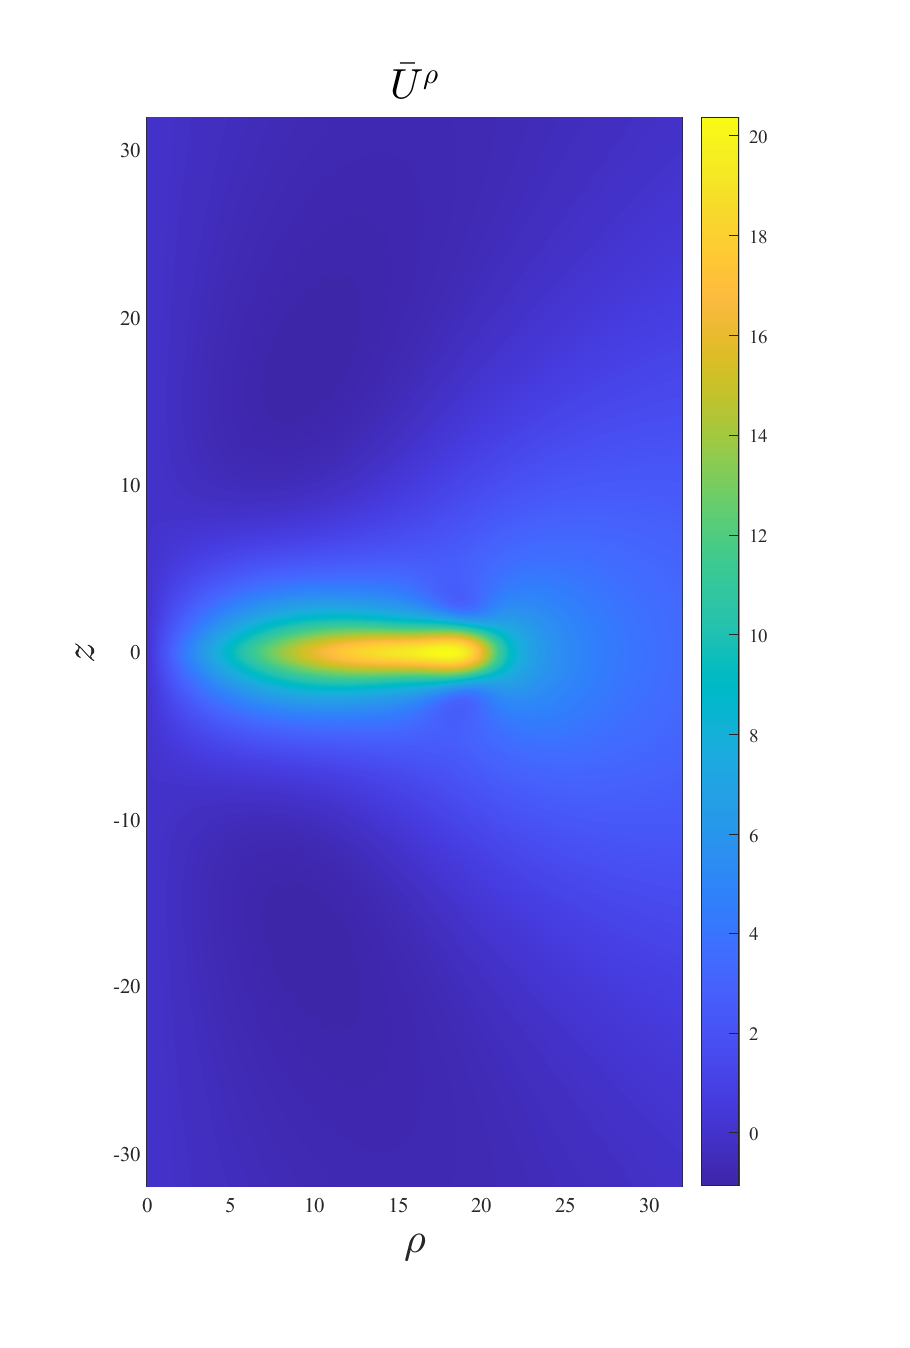
\includegraphics[width=\linewidth]{figures/Urho_pcolor.eps}
    \caption{$\overline{U}^\rho$}
  \end{subfigure}
  \begin{subfigure}{0.24\textwidth}
    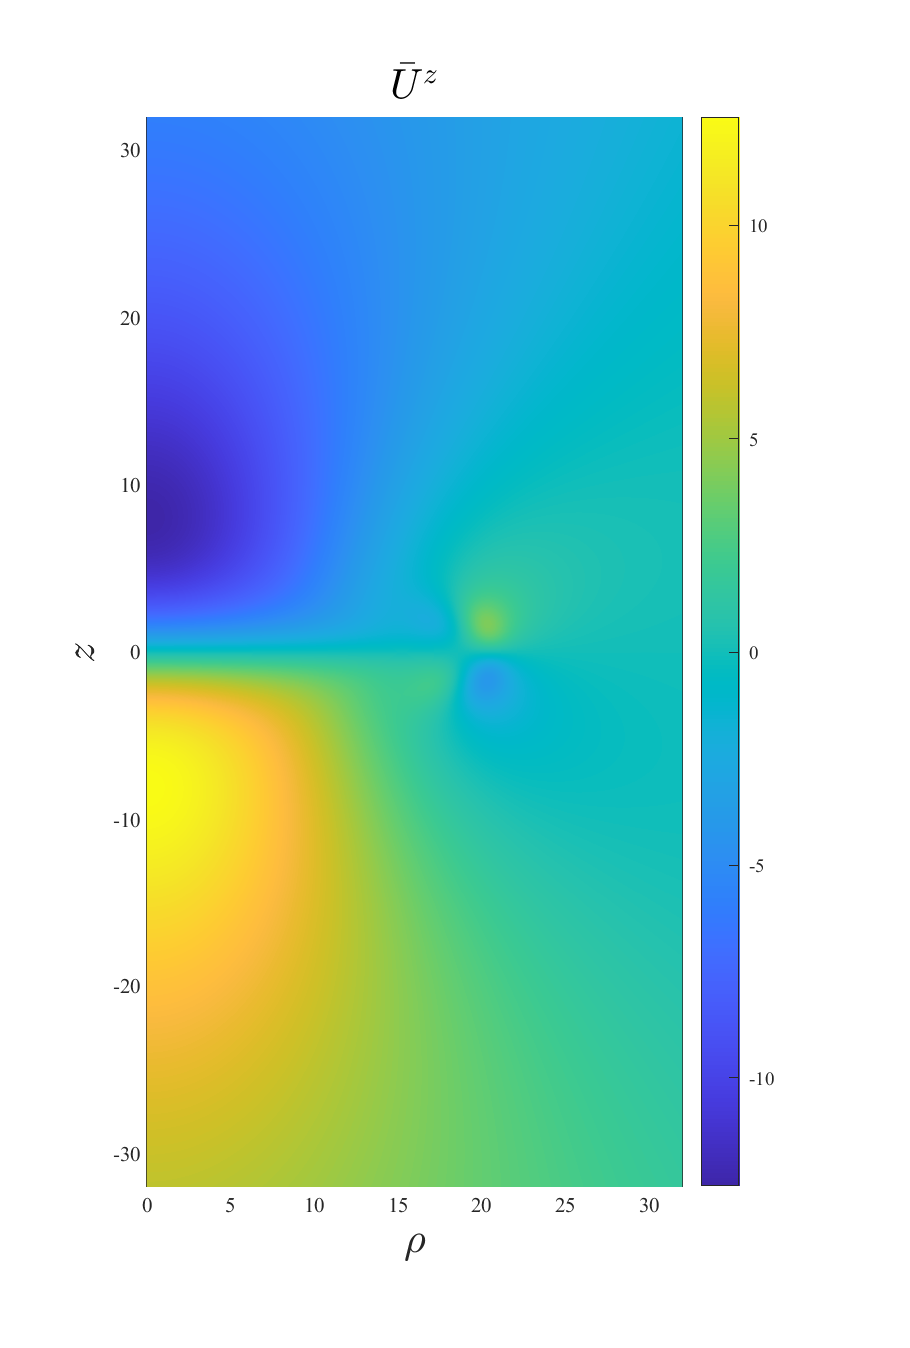
\includegraphics[width=\linewidth]{figures/Uz_pcolor.eps}
    \caption{$\overline{U}^z$}
  \end{subfigure}
  \begin{subfigure}{0.24\textwidth}
    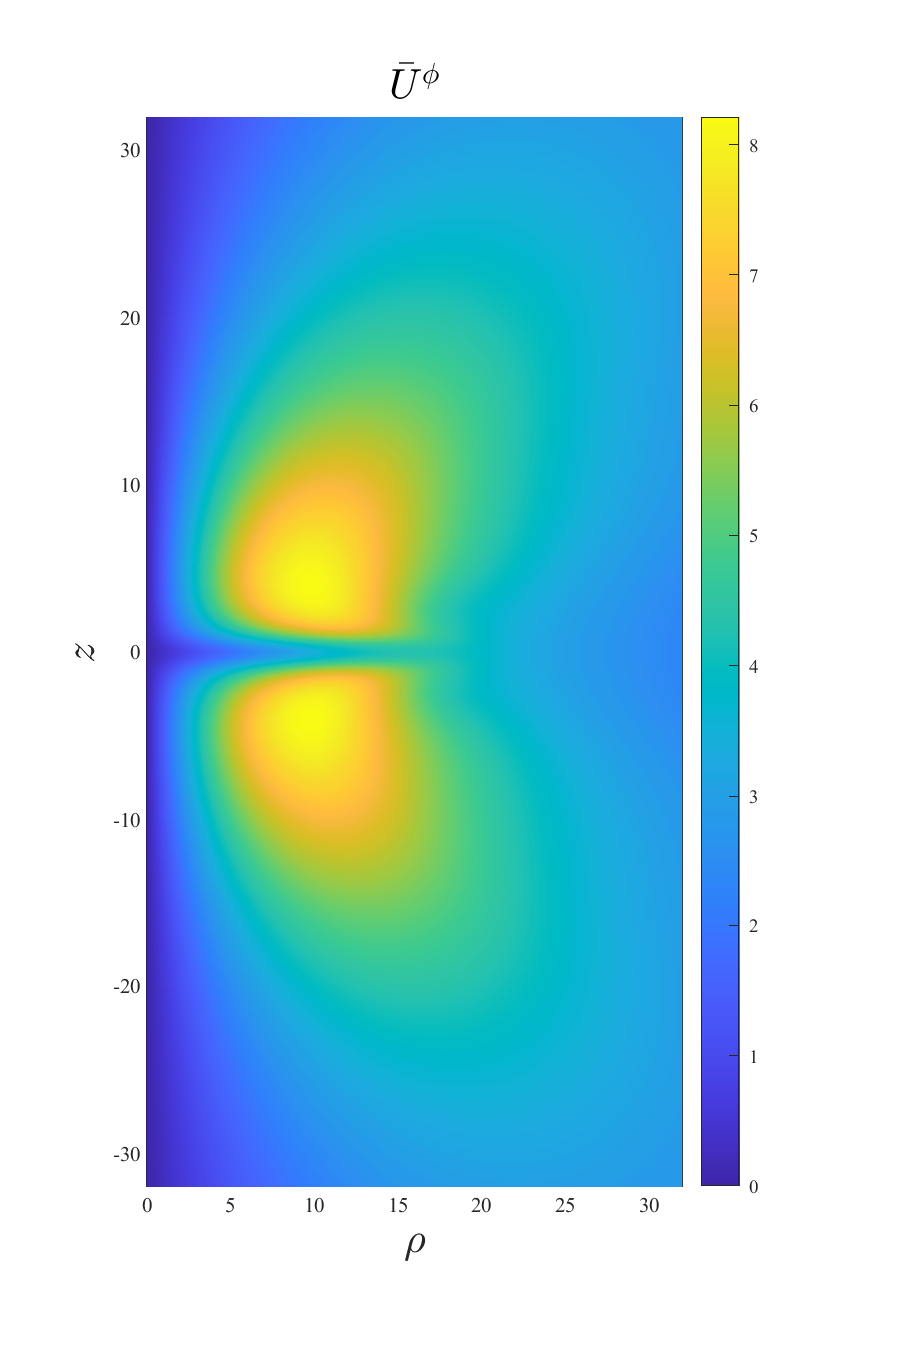
\includegraphics[width=\linewidth]{figures/Uphi_pcolor.eps}
    \caption{$\overline{U}^\phi$}
  \end{subfigure}
  \begin{subfigure}{0.24\textwidth}
    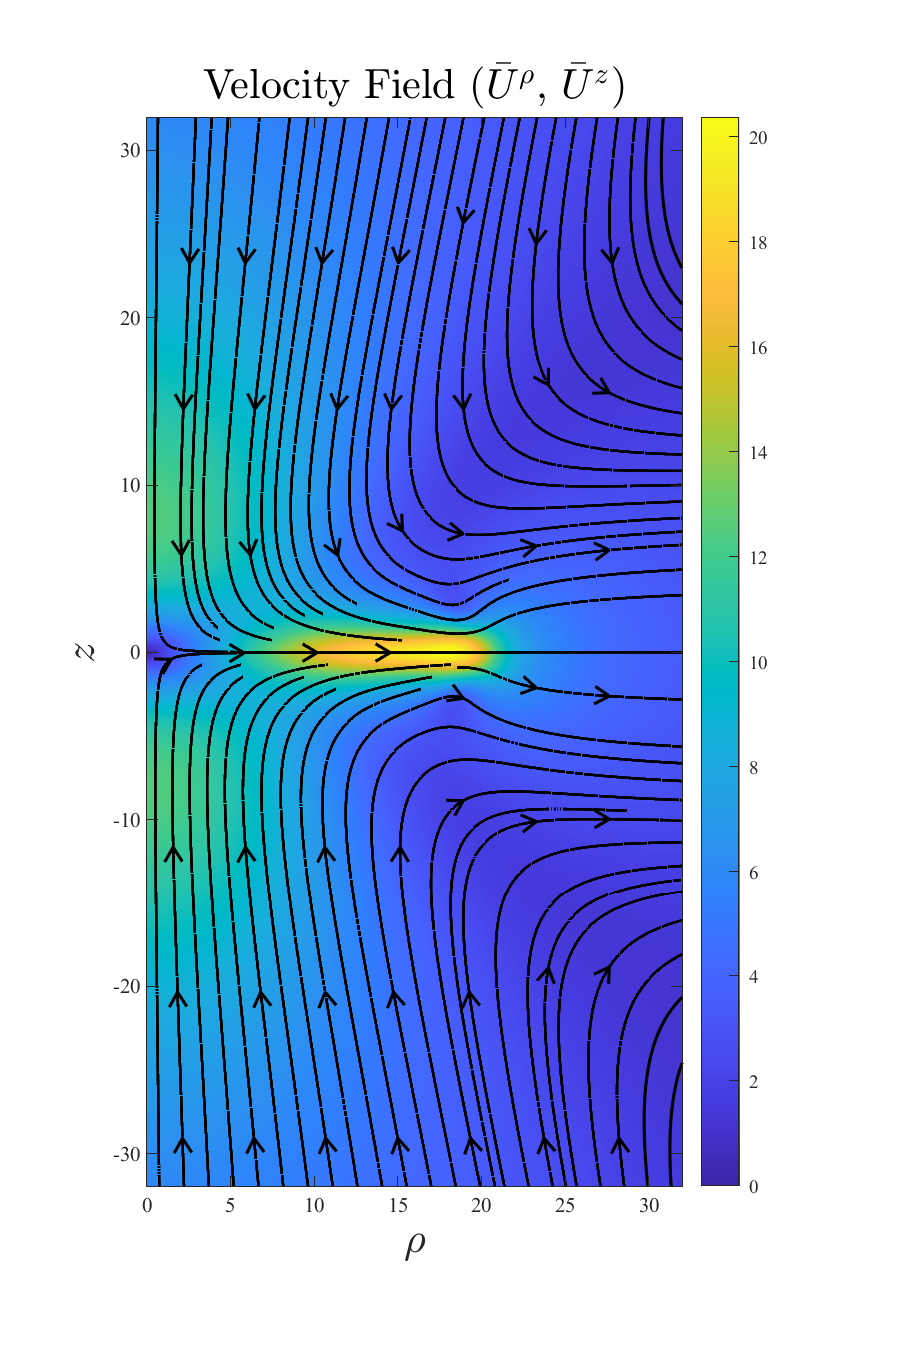
\includegraphics[width=\linewidth]{figures/Urho_Uz_stream_norm_pcolor.eps}
    \caption{$\overline{U}$ on the $\rho-z$ plane}
  \end{subfigure}
  \caption{Figures of $\overline{U}$}
  \label{fig:U figs}
\end{figure}

\begin{figure}[htbp]
  \centering
  \begin{subfigure}{0.24\textwidth}
    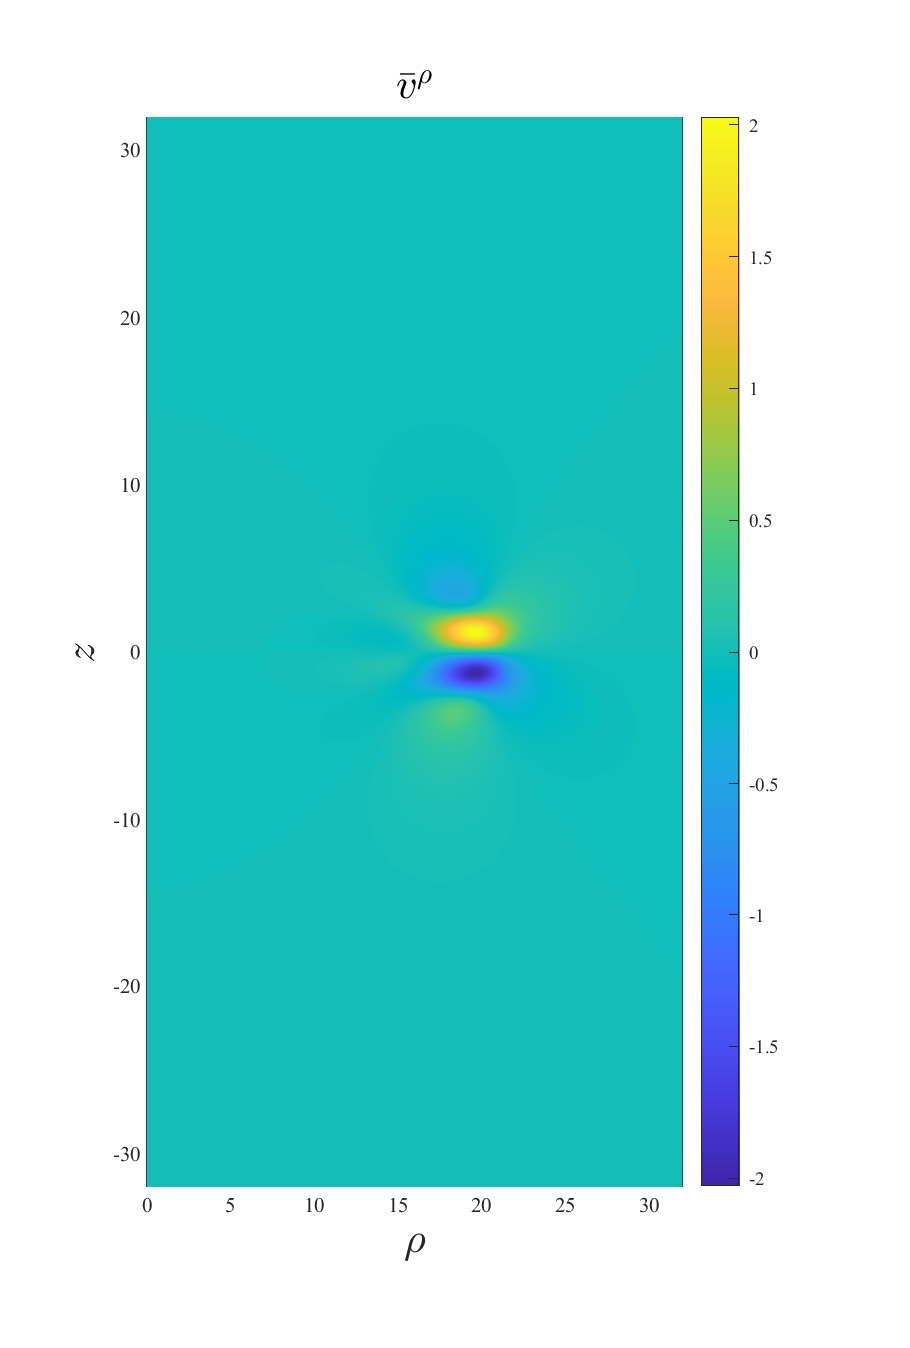
\includegraphics[width=\linewidth]{figures/vrho_pcolor.eps}
    \caption{$\overline{v}^\rho$}
  \end{subfigure}
  \begin{subfigure}{0.24\textwidth}
    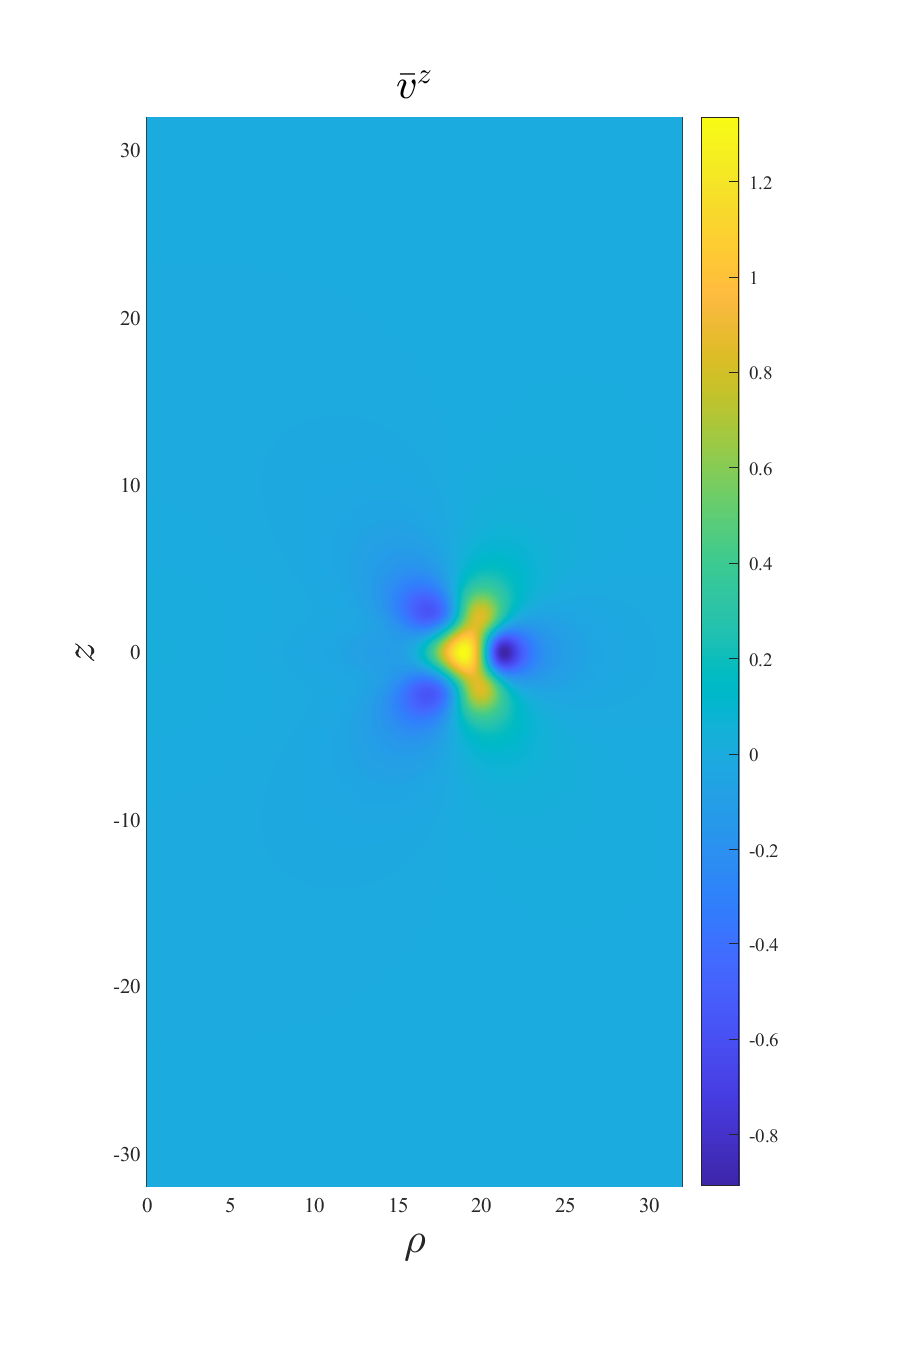
\includegraphics[width=\linewidth]{figures/vz_pcolor.eps}
    \caption{$\overline{v}^z$}
  \end{subfigure}
  \begin{subfigure}{0.24\textwidth}
    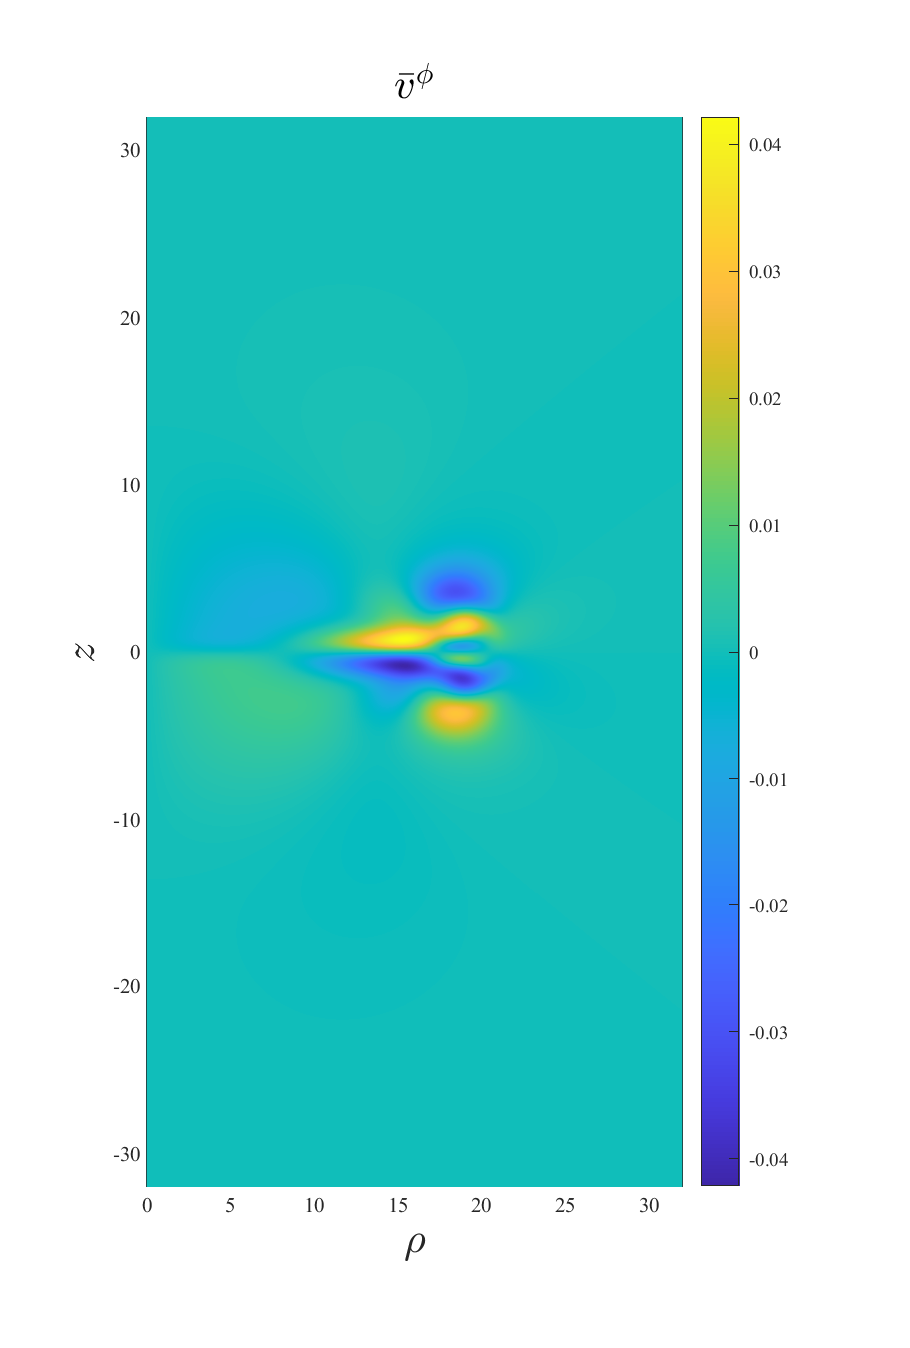
\includegraphics[width=\linewidth]{figures/vphi_pcolor.eps}
    \caption{$\overline{v}^\phi$}
  \end{subfigure}
  \begin{subfigure}{0.24\textwidth}
    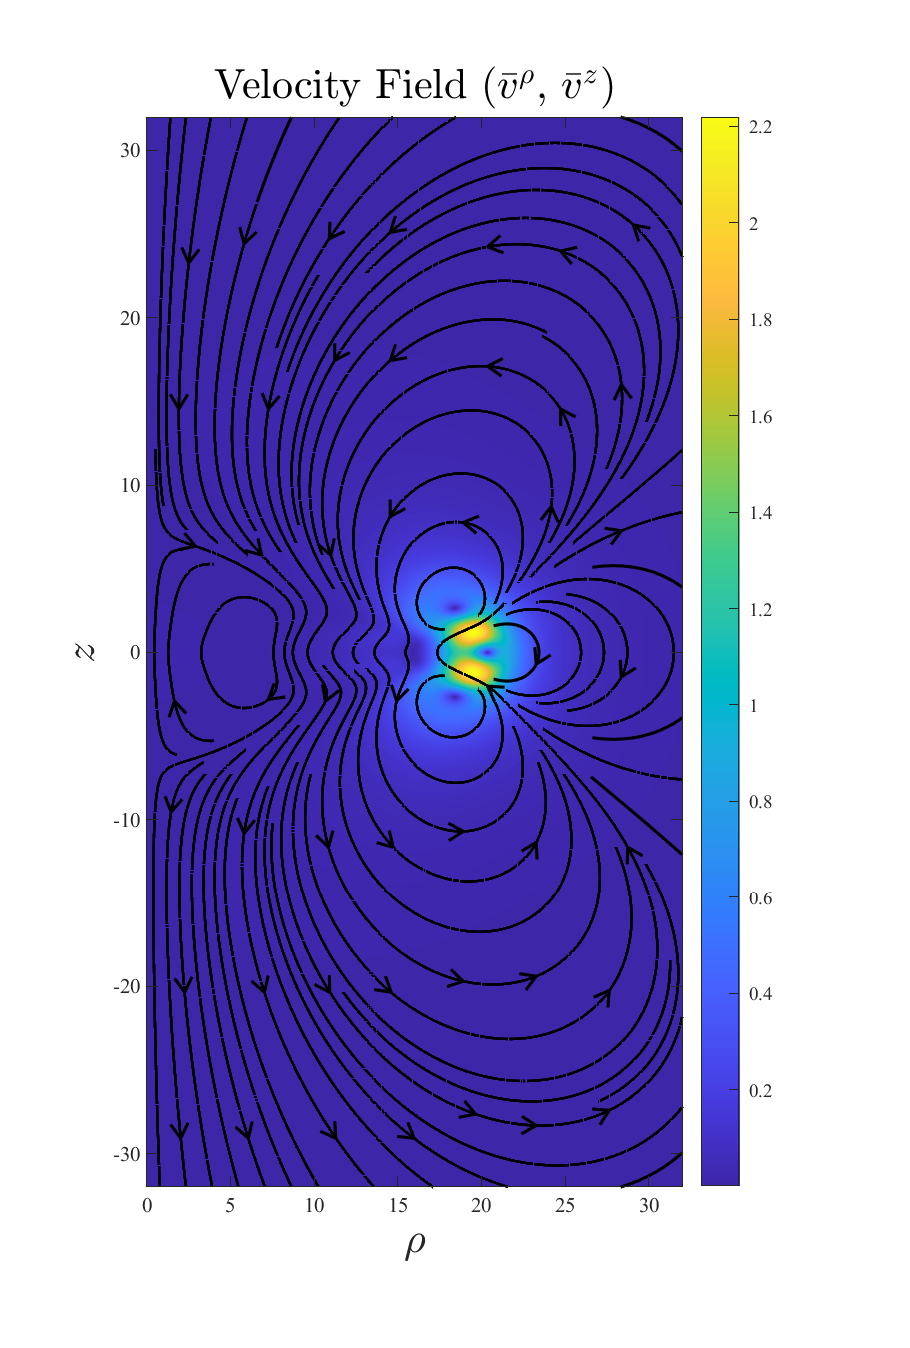
\includegraphics[width=\linewidth]{figures/vrho_vz_stream_norm_pcolor.eps}
    \caption{$\overline{v}$ on the $\rho-z$ plane}
  \end{subfigure}
  \caption{Figures of $\overline{v}$}
  \label{fig:v figs}
\end{figure}

\begin{figure}[htbp]
  \centering
  \begin{subfigure}{0.24\textwidth}
    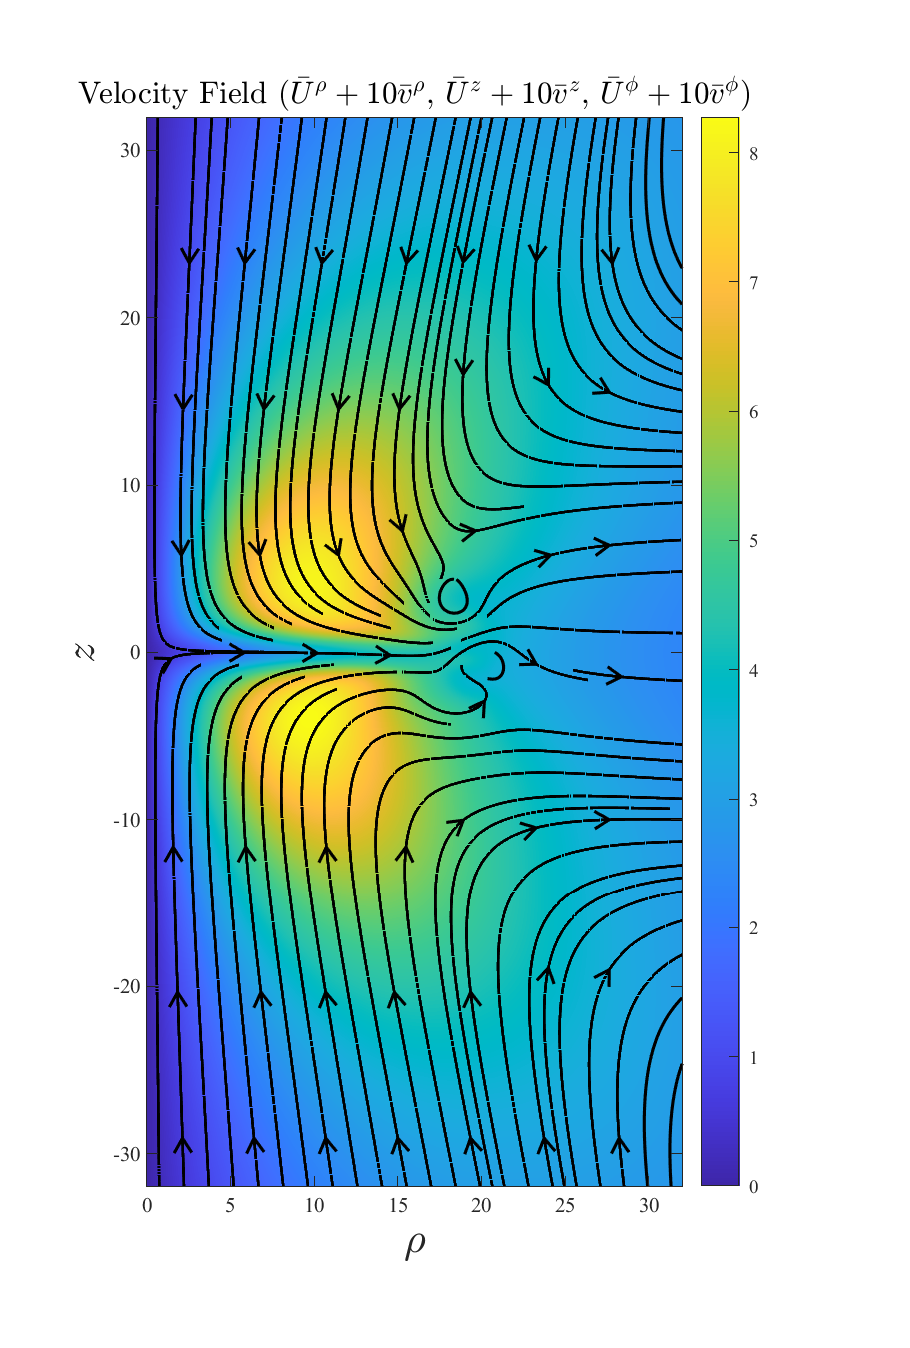
\includegraphics[width=\linewidth]{figures/Sum10rho_Sum10z_stream_Sum10phi_pcolor.eps}
    \caption{$\overline{U} + 10 \overline{v}$}
  \end{subfigure}
  \begin{subfigure}{0.24\textwidth}
    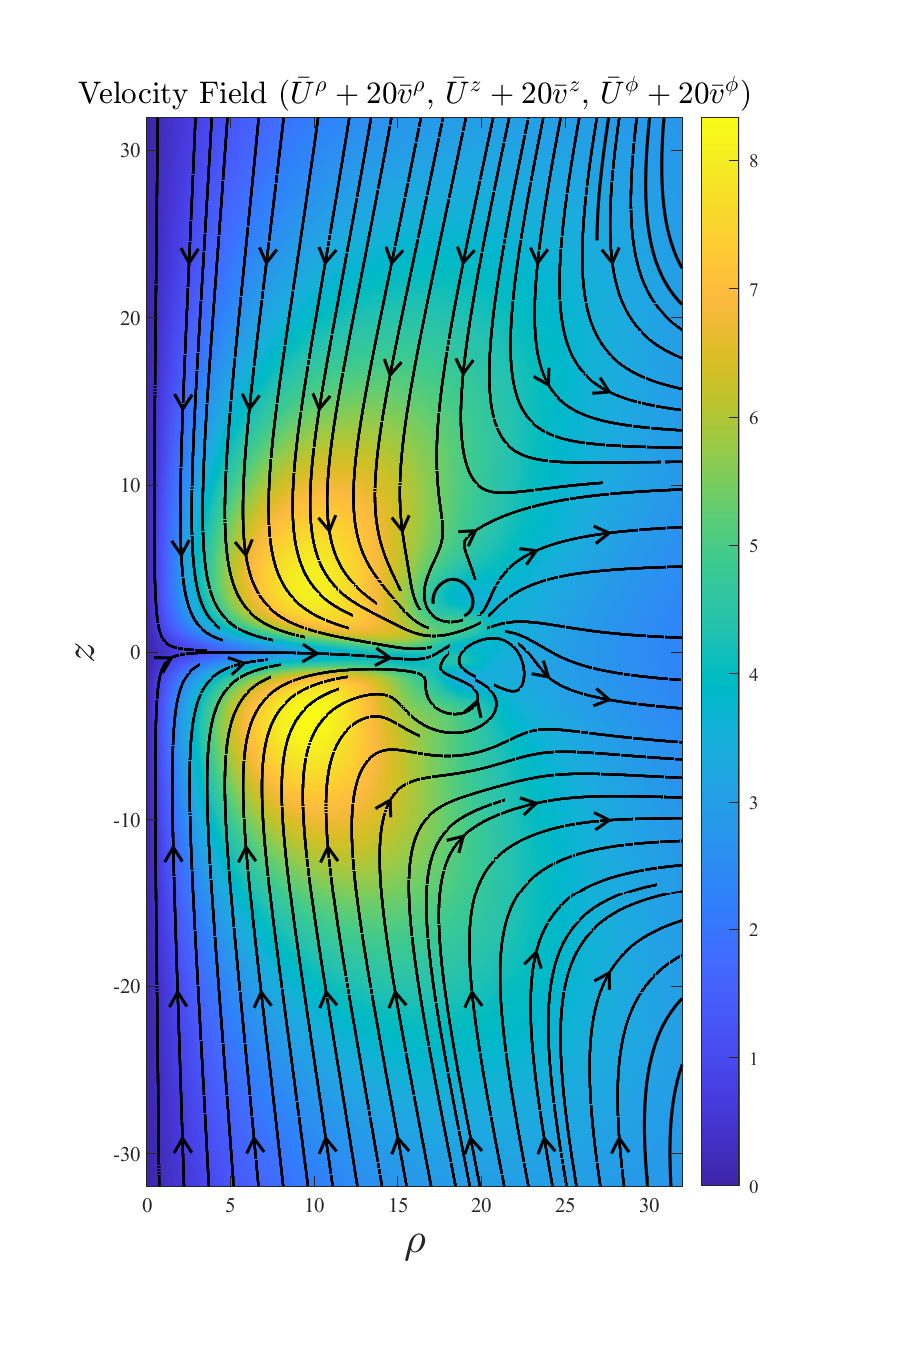
\includegraphics[width=\linewidth]{figures/Sum20rho_Sum20z_stream_Sum20phi_pcolor.eps}
    \caption{$\overline{U} + 20 \overline{v}$}
  \end{subfigure}
  \begin{subfigure}{0.24\textwidth}
    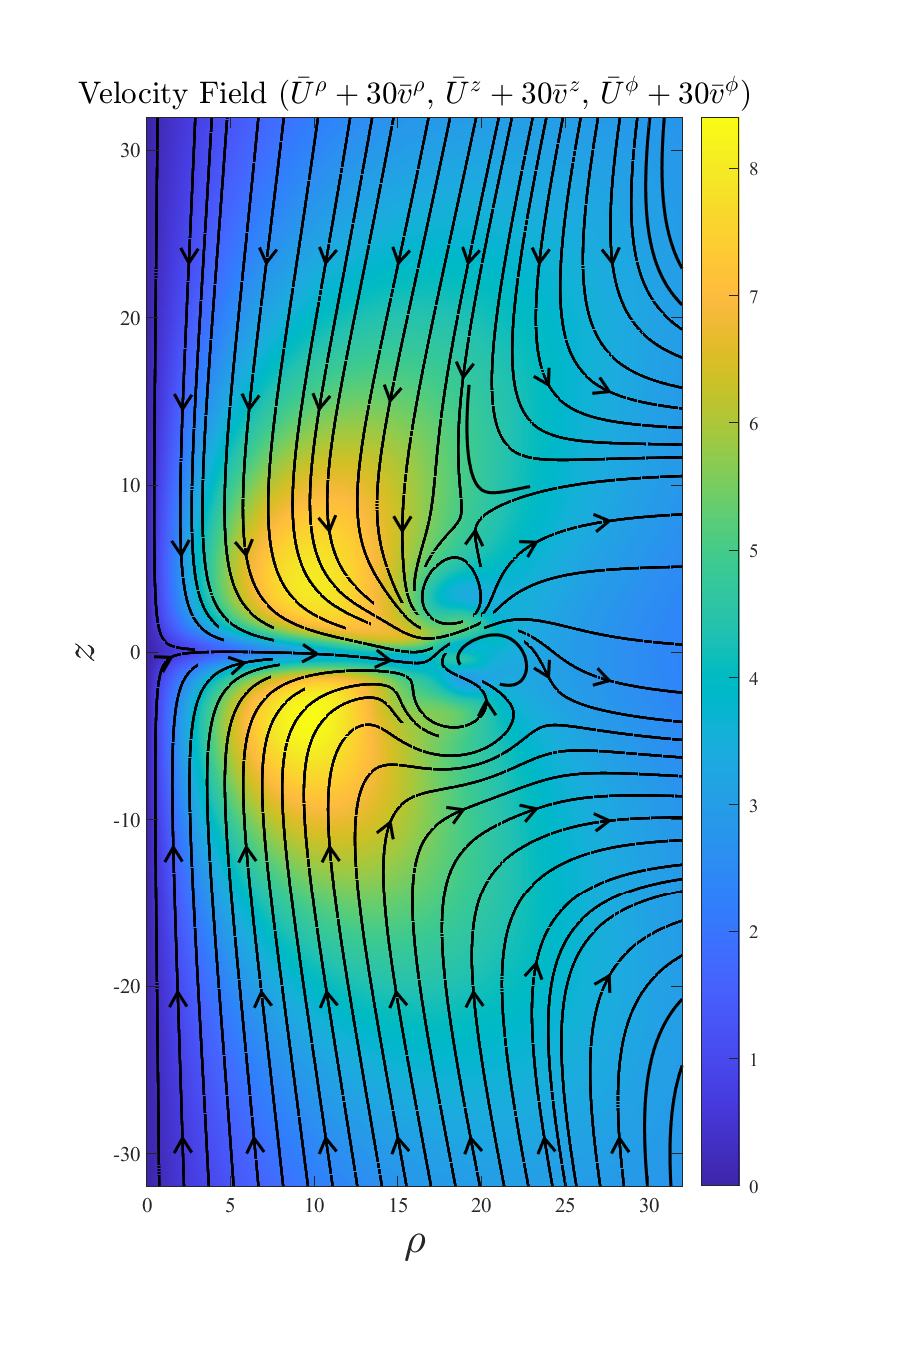
\includegraphics[width=\linewidth]{figures/Sum30rho_Sum30z_stream_Sum30phi_pcolor.eps}
    \caption{$\overline{U} + 30 \overline{v}$}
  \end{subfigure}
  \begin{subfigure}{0.24\textwidth}
    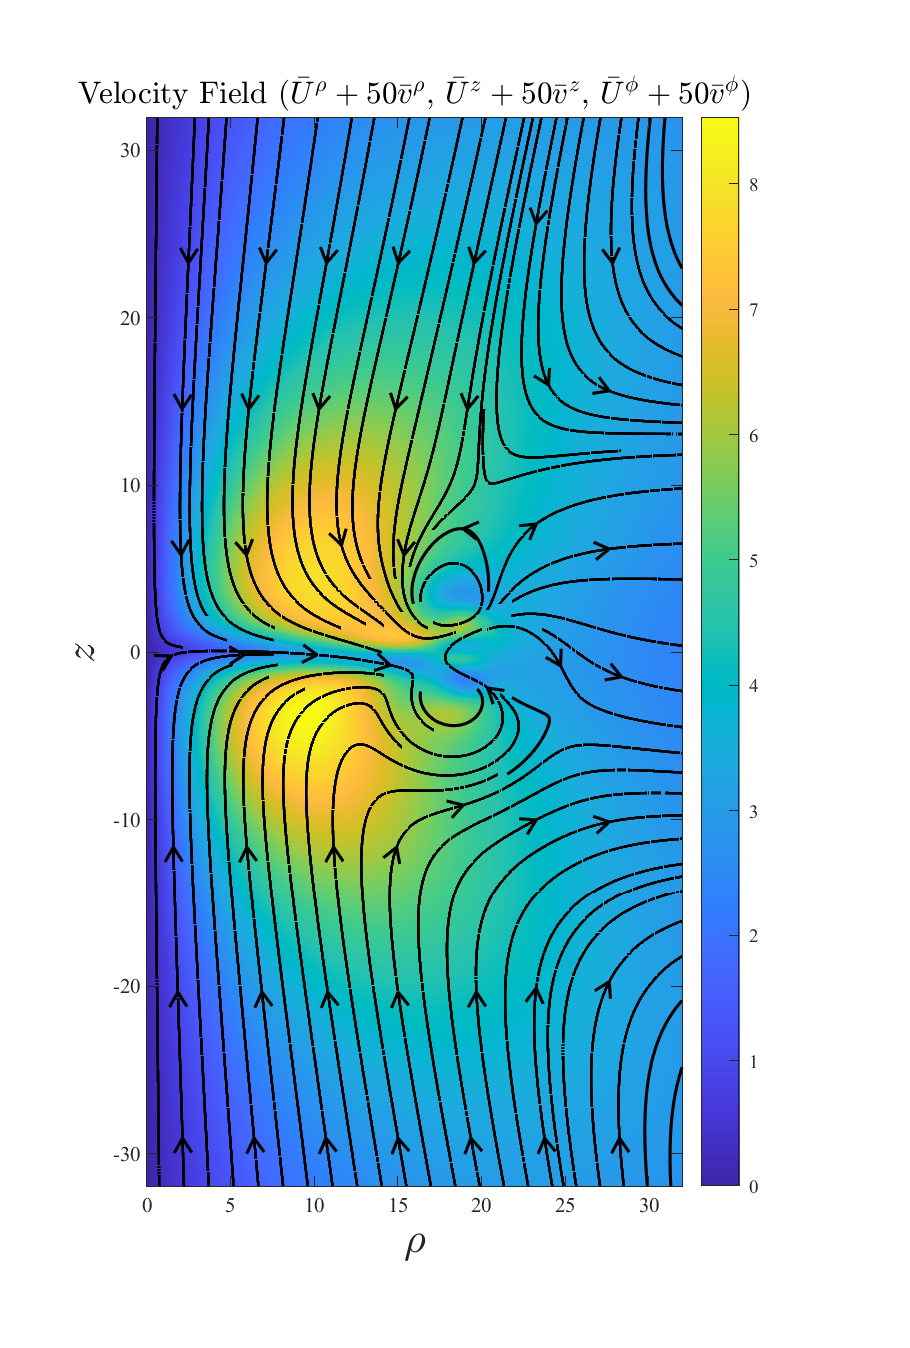
\includegraphics[width=\linewidth]{figures/Sum50rho_Sum50z_stream_Sum50phi_pcolor.eps}
    \caption{$\overline{U} + 50 \overline{v}$}
  \end{subfigure}
  \caption{Figures of $\overline{U} + \sigma \overline{v}$ with different $\sigma$}
  \label{fig:Uv figs}
\end{figure}

\begin{figure}[htbp]
  \centering
  \begin{subfigure}{0.24\textwidth}
    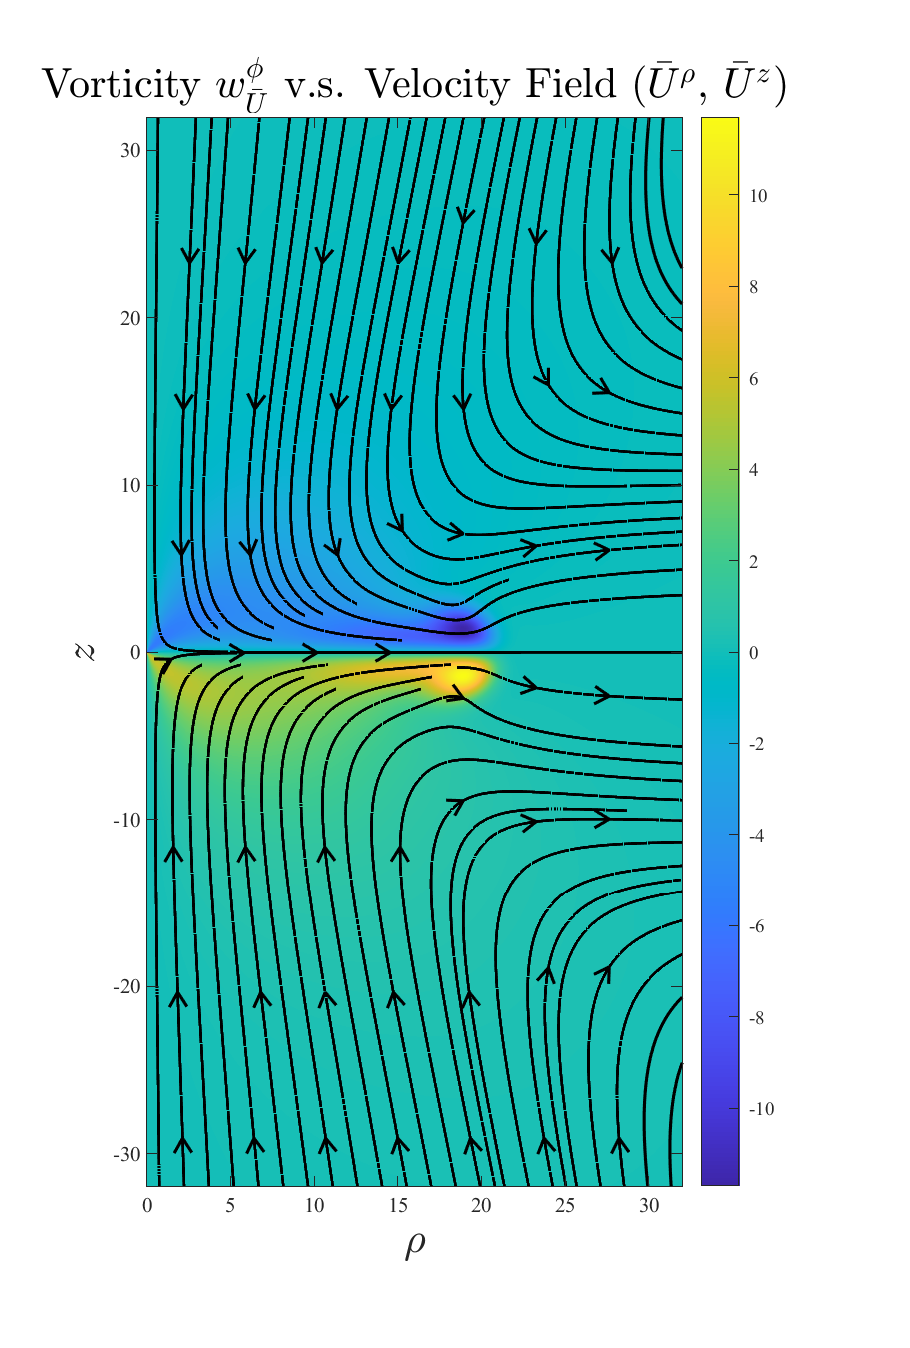
\includegraphics[width=\linewidth]{figures/w_Uphi_pcolor_Urho_Uz_stream.eps}
    \caption{$\omega_\phi^U$}
  \end{subfigure}
  \begin{subfigure}{0.24\textwidth}
    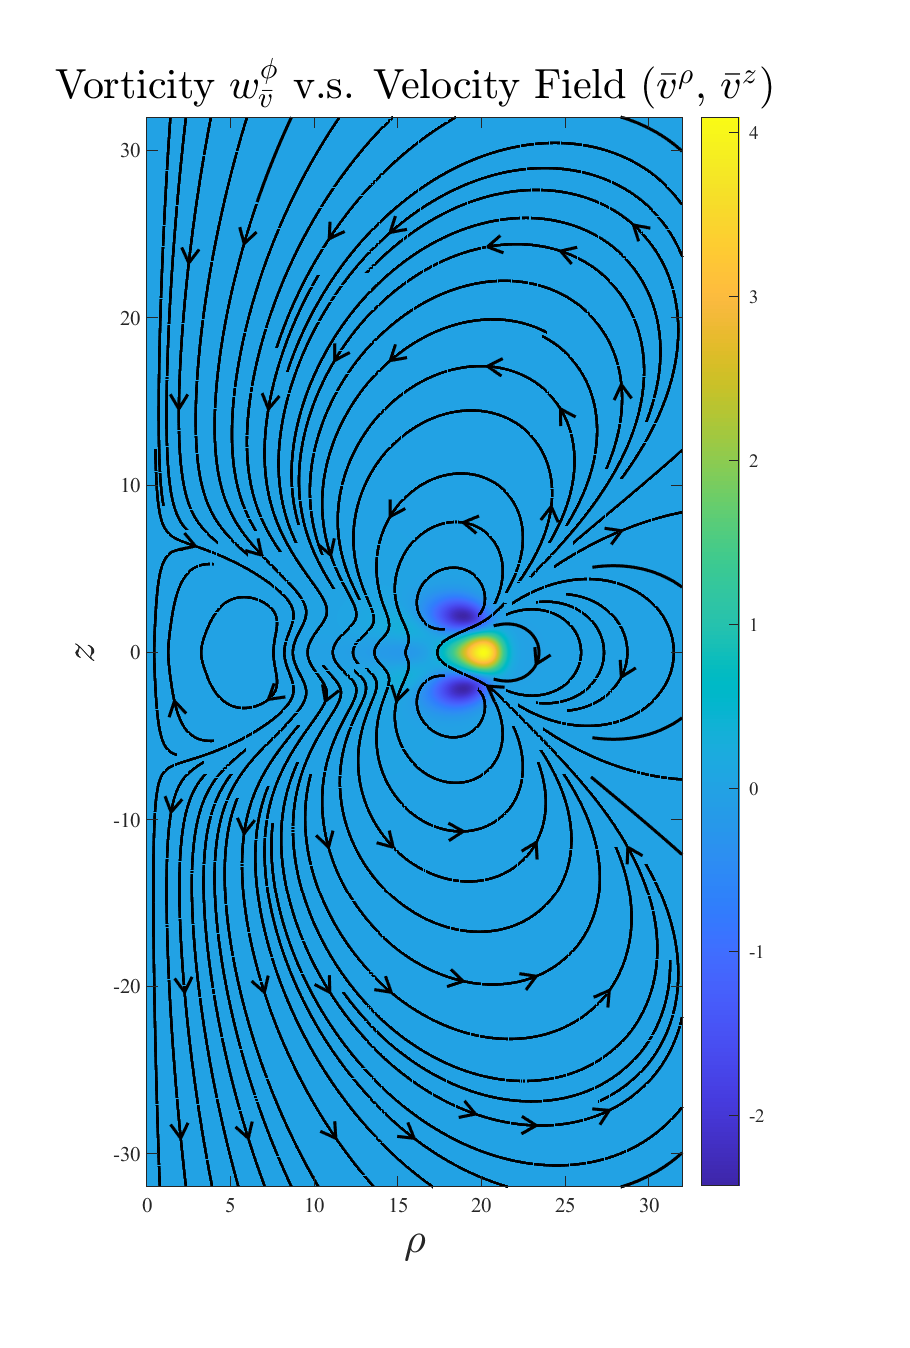
\includegraphics[width=\linewidth]{figures/w_vphi_pcolor_vrho_vz_stream.eps}
    \caption{$\omega_\phi^v$}
  \end{subfigure}
  \begin{subfigure}{0.24\textwidth}
    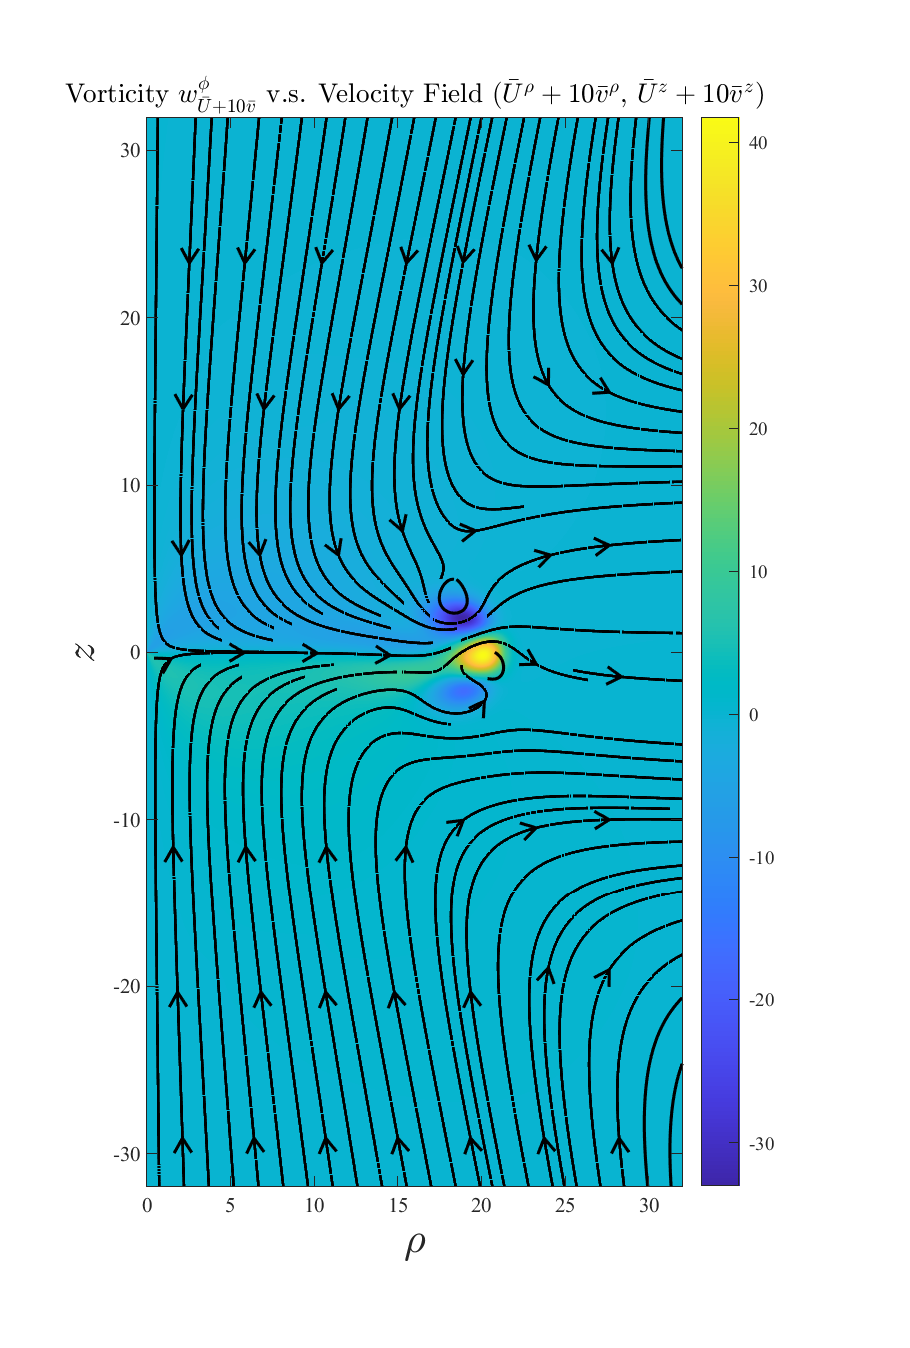
\includegraphics[width=\linewidth]{figures/w_Sum10phi_pcolor_Sum10rho_Sum10z_stream.eps}
    \caption{$\omega_\phi^U + 10 \omega_\phi^v$}
  \end{subfigure}
  \caption{Vorticity of $\overline{U}, \overline{v}$ and $\overline{U} + 10 \overline{v}$}
  \label{fig:omega figs}
\end{figure}

\section{Finite Rank Approximation}\label{Sec:numfr}

In this section, we construct the finite rank approximation for $L_2 = - \Pi
(U \cdot Q)$. Recall the decomposition of $\nabla \overline{U}$:
\[ Q_s = \frac{\nabla \overline{U} + \nabla^T \overline{U}}{2}, \quad Q_s +
   \eta_1 I = Q_{+} - Q_{-}, \quad Q_{+} \succeq 0, \quad Q_{-} \succeq 0. \]
Here, $Q_{-}$ is the negative part of $Q_s + \eta_1 I$. In previous sections, we
choose $Q = Q_{-}$. We truncate the domain $\Omega = [0, R_0] \times \left[ 0,
\frac{\pi}{2} \right]$ with $R_0 = 32$ and verify that outside $\Omega$, we
have $\lambda_{\max} (Q_s) < 0.199$. Thus, we set $\eta_1 = 0.199$ so that the
support of $Q_{-}$ is fully contained in $\Omega$.

Although it is natural to take $Q = Q_{-}$, this choice has the drawback that
$Q$ is not smooth, which complicates the future error analysis of numerical
integrals. Fortunately, we only need $Q$ to satisfy
\begin{equation}
  Q_s + \eta_1 I + Q \succeq 0. \label{eq:Q cond}
\end{equation}
Therefore, we design a smooth matrix function $Q (x)$ on $\Omega$ that meets
this condition. The algorithm is described in Section \ref{sec:def Q}. Next,
we construct an appropriate basis to approximate functions defined on $\Omega$
in Section \ref{subSec:numfr} and solve an eigenvalue problem to build
$L_{\tmop{ap}}$ in Section \ref{sec:Q eig}. Finally, in Section \ref{sec:inv
L2}, we solve
\[ L \phi_i = Q \psi_i, \]
to define the operator $G$.

\subsection{Construction of $Q$}\label{sec:def Q}

We first construct $Q$. Since $Q$ is a symmetric matrix function, it has 6
independent entries: $Q_{11}, Q_{12}, Q_{13}, Q_{22}, Q_{23}, Q_{33}$. Each
entry satisfies the same boundary conditions as the corresponding entry of
$Q_s$ on the three sides of the domain boundary:
\[ \theta = 0, \frac{\pi}{2} \infixand r = 0. \]
Specifically, if $Q_{s, i j} = 0$ on a particular part of the boundary (say,
$r = 0$), then we impose the Dirichlet boundary condition $Q_{i j} = 0$ on
that same boundary segment. On the remaining boundary segments, where $Q_{s, i
j}$ does not vanish, we instead impose the Neumann boundary condition
$\partial_n Q = 0$. Consequently, $Q$ satisfies:
\[ \begin{array}{l}
     \partial_r Q_{11} (0, \theta) = \partial_r Q_{12} (0, \theta) = Q_{13}
     (0, \theta) = \partial_r Q_{22} (0, \theta) = Q_{23} (0, \theta) = Q_{33}
     (0, \theta) = 0,\\
     \partial_{\theta} Q_{11} (r, 0) = Q_{12} (r, 0) = Q_{13} (r, 0) =
     \partial_{\theta} Q_{22} (r, 0) = Q_{23} (r, 0) = \partial_{\theta}
     Q_{33} (r, 0) = 0,\\
     \partial_{\theta} Q_{11} \left( r, \frac{\pi}{2} \right) = Q_{12} \left(
     r, \frac{\pi}{2} \right) = \partial_{\theta} Q_{13} \left( r,
     \frac{\pi}{2} \right) = \partial_{\theta} Q_{22} \left( r, \frac{\pi}{2}
     \right) = Q_{23} \left( r, \frac{\pi}{2} \right) = \partial_{\theta}
     Q_{33} \left( r, \frac{\pi}{2} \right) = 0.
   \end{array} \]
On $r = R_0$, we need to impose the Dirichlet boundary condition $Q = 0$ since
the support of $Q$ is fully contained in $\Omega$. Guided by these boundary
conditions, we select the corresponding trigonometric basis to approximate
each entry. For instance, $Q_{11}$ is approximated by
\[ Q_{11} = \sum_{l = 1}^L \sum_{m = 1}^M q_{11, l m} \cos \left( \frac{(2 m +
   1) \pi r}{2 R_0} \right) \cos (2 l \theta) . \]
A na{\"i}ve approach would be to apply the discrete Fourier transform to $Q_{-}$
and truncate the series. However, this does not ensure $Q_s + \eta_1 I + Q
\succeq 0$. To address this, we first select a slightly smaller $\eta_0 =
0.19$ and  reconstruct $Q$ using the
same idea of a truncation of Fourier series. As long as $L, M$ are sufficiently large, we obtain \eqref{eq:Q
cond}.

This method, however, typically requires very large $L, M$, which is
undesirable. To improve efficiency, we fix $L = 150, M = 300$ and use an iterative method. We initialize
$Q_0 = 0$ with $\eta_0 = 0.19$. For every iteration $Q_i$, we calculate
\[ \delta Q_{-, i} \assign \text{negative part of}  \,(Q_s + \eta_0 I + Q_i) .
\]
If $\| \lambda_{\max} (\delta Q_{-, i}) \|_{L^{\infty}} < \delta_{\eta}
\assign \eta_1 - \eta_0$, we terminate the iteration.

Otherwise, we approximate $\delta Q_{-, i}$ by a trigonometric polynomial,
denoted $\delta Q_i$. Specifically, to guarantee that $\delta Q_i$ is positive, we take $\delta Q_i$ to be the Fej{\'e}r
transform of $\delta Q_{-, i}$ in both $r$ and $\theta$, which is equivalent
to convolving with the kernel:
\[ K_N (x) = \frac{1}{N} \left( \frac{1 - \cos (N x)}{1 - \cos (x)} \right) .
\]
This algorithm is particularly easy to implement because convolution acts as a
Fourier multiplier. Thus, it suffices to compute the Fourier transform of the
kernel, whose coefficients are given by
\[ \mathcal{F}_x K_N^j = \left( 1 - \frac{| j |}{N} \right), \quad | j | < N,
\]
and vanish for $| j | \geqslant N$. We then update $Q_i$ by
\[ Q_{i + 1} = Q_i + \delta Q_i . \]
Finally, we can obtain a smooth function $Q$ satisfying \eqref{eq:Q cond} within 5 iterations.

\subsection{Construction of spectral basis}\label{subSec:numfr}

Since the $Q$-norm $\| \cdummy \|_Q$ is controlled by the standard $L^2$-norm,
we begin by considering the following eigenvalue problem in the Rayleigh quotient
form:
\begin{equation}
  \lambda_n^s = \sup_{\dim (V_n) = n - 1} \inf_{u \neq 0, u \in V, u \bot V_n}
  \frac{\| \nabla u\|^2_{\Omega}}{\|u\|^2_{\Omega}}, \label{rayleigh}
\end{equation}
where $V$ is the space of admissible functions, namely divergence-free
axisymmetric functions. We obtain a sequence of $\lambda_n^s$ in ascending
order with associated eigenfunctions $\psi_n^s$. These eigenfunctions will
constitute our spectral basis.

The solutions to this eigenvalue problem admit explicit representations in
terms of Bessel functions and spherical harmonics, as established in the
following lemma.

\begin{lemma}
  \label{lem:lap eig}Consider the eigenvalue problem \eqref{rayleigh} with
  $\Omega$ being the unit ball in 3D. The first eigenpair is
  \[ \lambda_0^s = 0, \quad \psi_0^s = (\cos \theta, - \sin \theta, 0) . \]
  For $s \geqslant 1$, the remaining eigenvalues can be written as
  \[ \lambda_n^s = (\alpha_{l, m}^i)^2, \quad l \geqslant 1, \quad m \geqslant
     1, \quad i = Y \infixor Z. \]
  {\tmstrong{Case 1: $i = Z$}}
  
  Here, $\alpha_{l, m}^Z > 0$ denotes the m-th zero of the equation for $r$:
  \begin{equation}
    rJ_{l + \frac{1}{2}}' (r) - \frac{1}{2} J_{l + \frac{1}{2}} (r) = 0,
    \label{eq:alphaZ}
  \end{equation}
  where $J_{\nu}$ is the Bessel function of the first kind. The corresponding
  eigenfunction is
  \[ \psi_n^s = \psi_{ml}^Z = \frac{J_{l + \frac{1}{2}}  (\alpha^Z_{ml}
     r)}{\sqrt{r}} Z_l (\theta) . \]
  {\tmstrong{Case 2: $i = Y$}}
  
  Here, $\alpha_{l, m}^Y > 0$ denotes the m-th zero of the equation for $r$:
  \begin{equation}
    (r^2 - l (l - 1) (l + 2)) r \tilde{j}_l' (r) + (r^2 - l (l - 1))  (r^2 -
    (l - 1) (l + 2))  \tilde{j}_l (r) = 0, \label{eq:alphaY}
  \end{equation}
  where
  \[ \tilde{j}_l (r) \assign \frac{J_{l + \frac{1}{2}} (r)}{r^{\frac{3}{2}}} .
  \]
  The corresponding eigenfunction is
  \[ \psi_n^s = \psi_{ml}^Y = (B_{ml}  \tilde{j}_l (\alpha^Y_{ml} r) + lA_{ml}
     r^{l - 1}) Y_l (\theta) + \left( \frac{B_l}{\mu_l} (r \alpha^Y_{ml} 
     \tilde{j}_l' (\alpha^Y_{ml} r) + 2 \tilde{j}_l (\alpha^Y_{ml} r)) + A_l
     r^{l - 1} \right) X_l (\theta), \]
  with
  \[ A_{ml} = - ((\alpha^Y_{ml})^2 - (l - 1) (l + 2))  \tilde{j}_l
     (\alpha^Y_{ml}), \quad B_{ml} = (\alpha^Y_{ml})^2 - l (l - 1)  (l + 2) .
  \]
\end{lemma}

The proof of the lemma is given in Appendix \ref{eig cons}.

\begin{remark}[Scaling and Parity]
  In our setting, $\Omega = B_0 (R_0)$ with $R_0 = 32$. The eigenvalues and
  eigenfunctions can be obtained by rescaling with respect to $R_0$.
  Specifically, the eigenvalues are $\frac{\lambda^s_n}{R_0^2}$ and the
  eigenvectors are $\psi_n^s \left( \frac{r}{R_0}, \theta \right)$. Recall
  that, since $U$ and $v$ also satisfy different boundary conditions, in the
  vector spherical harmonics expansion as in Section \ref{sec:div-free}, only
  even $l$ or only odd $l$ appear. Hence, we retain only eigenpairs of certain
  parities in the construction. We denote by $\lambda_k^{s, U}$ the $k$-th
  smallest eigenvalue among all $\frac{\lambda^s_n}{R_0^2}$ with even
  eigenfunctions $\psi_k^{s, U} = \psi_n^s \left( \frac{r}{R_0}, \theta
  \right)$, and similarly define $\lambda_k^{s, v}$ and $\psi_k^{s, v}$.
\end{remark}

Let $V_N^i$ denote the space spanned by the first $N$ eigenvectors $\psi_n^{s,
i}$ for $i = U, v$ respectively. We define the projection $I^i_N$ as
\begin{equation}
    I^i_N \psi = \sum_{k = 1}^N \langle \psi, \psi_k^{s, i} \rangle \psi_k^{s,
   i} . \label{eq:I def}
\end{equation}
It is both the $L^2$ and $H^1$ projection onto $V_N^i$. By \eqref{rayleigh},
it satisfies
\[ \| \psi - I^i_N \psi \|_{L^2} \leqslant \frac{1}{\lambda_{N + 1}^{c, i}} \|
   \psi \|_{H^1}, \quad \| \psi - I^i_N \psi \|_{L^2} \leqslant \| \psi
   \|_{L^2}, \quad \forall \psi \in V. \]
Recall the constant $K_5^i$ from \eqref{k5}, we can set
\[ K_5^i = \frac{\| \lambda_{\max} (Q)\|_{\infty}}{\eta_2 + \lambda_{N
   + 1}^{s, i}} . \]
Numerically, we find $\| \lambda_{\max} (Q)\|_{\infty} \leqslant 4.5$. Since
we hope $K_5^i \leqslant 0.45$, we need to choose $N$ such that
$\lambda_{N + 1}^{s, i} > 10$. Thus, we take $N = 1257$ for $U$ and $N = 1260$
for $v$ to ensure the required bound.

Finally, note that it is necessary to compute all eigenvectors corresponding
to eigenvalues smaller than 10. In particular, we need the following estimate
to guarantee that all eigenvalues below 10 have been identified: (This lemma
is still for the unscaled eigenvalue $\lambda^s_n$).

\begin{lemma}
  \label{lem:zeros}Let $0 = \beta_{l, 0} < \beta_{l, 1} < \beta_{l, 2} <
  \cdots$ denote the zeros of $J_{l + \frac{1}{2}} (k)$ and $\gamma = \sqrt{l
  (l - 1)  (l + 2)}$.
  \begin{itemizedot}
    \item If $l = 1$, define $\tilde{\beta}_{1, j} = \beta_{1, j}$;
    
    \item If $l \geqslant 2$ and $\gamma \neq \beta_{l, j}$ for any $j > 0$,
    denote $\tilde{\beta}_{l, j}$ as the sequence obtained by sorting
    $\{\beta_{l, j}, \gamma\}$ in an ascending order.
  \end{itemizedot}
  Let $s_l$ be the unique positive root of:
  \[ Q_l (s) = s^3 - 4 l^2 s^2 + l (l - 1)  (6 l^2 + 11 l + 7) s - 3 l (l -
     1)^2  (l + 1)^2  (l + 2), \]
  and $t_l = \sqrt{l (l + 1)}$. Assume that $\sqrt{s_l}$ is not a root of
  \eqref{eq:alphaY} and that $t_l$ is not a root of \eqref{eq:alphaZ}.
  
  Then the following statements hold:
  \begin{enumeratenumeric}
    \item The equation \eqref{eq:alphaY} has exactly one root on every
    interval $(\tilde{\beta}_{l, j}, \tilde{\beta}_{l, j + 1})$ for $j
    \geqslant 0$.
    
    \item The equation \eqref{eq:alphaZ} has exactly one root on every
    interval $(\beta_{l, j}, \beta_{l, j + 1})$ for $j \geqslant 0$.
    
    \item The first zeros $\alpha_{l, 1}^Y$ and $\alpha_{l, 1}^Z$ satisfy the
    lower bounds:
    \[ \alpha_{l, 1}^Y \geqslant \sqrt{s_l}, \quad \alpha_{l, 1}^Z \geqslant
       t_l . \]
  \end{enumeratenumeric}
\end{lemma}

The proof of the lemma is given in Appendix \ref{eig cons}. In practice, we
use the lower bounds of $\alpha_{l, 1}^Y$ and $\alpha_{l, 1}^Z$ to determine
the largerst index $l$ required, denoted by $l_{\max}$. For every $1 \leqslant
l \leqslant l_{\max}$, we then search all the intervals $(\beta_{l, j},
\beta_{l, j + 1})$ and $(\widetilde{\beta}_{l, j}, \widetilde{\beta}_{l, j + 1})$ for
$\alpha_{l, 1}^Z$ and $\alpha_{l, 1}^Y$, respectively, until the left endpoint
of the interval exceeds the prescribed threshold.

\subsection{Eigenvalue problem}\label{sec:Q eig}

We subsequently solve the finite-dimensional eigenvalue problem numerically:
\[ \langle \psi, Q \psi_n^{Q, i} \rangle_{\Omega} = \lambda^{Q, i}_n  \langle
   \psi, \psi_n^{Q, i} \rangle_E, \quad \forall \psi \in V_N^i , \]
on the space $V_N^i$. Recall that $\psi_k^{s, i}$ are orthogonal in $L^2$ and
$H^1$. We will normalize them to obtain an orthonormal basis in $E$ as
$\widetilde{\psi}_k^{s, i}$ and compute the matrix:
\begin{equation}
  (A_Q^i)_{k, j} = \langle \widetilde{\psi}_k^{s, i}, Q \widetilde{\psi}_j^{s, i}
  \rangle_{\Omega}, \label{def:aq}
\end{equation}
using numerical integration, and solve the resulting eigenvalue problem:
\[ A_Q^i \psi^{Q, i}_n = \lambda^{Q, i}_n \psi^{Q, i}_n . \]
Here, by an abuse of notation, we use $\psi^{Q, i}_n$ to denote both the
eigenvector and its coordinates in the basis $\widetilde{\psi}_k^{s, i}$.

We solve the matrix eigenvalue problem numerically to determine all
eigenvalues $\lambda^{Q, i}_n \geqslant 0.46$. Numerical computations yield:
\[ \lambda^U_{20} \approx 0.456 < 0.46, \quad \lambda^v_{25} \approx 0.453 <
   0.46. \]
These numerics determine the rank used in the finite-rank operator. The
computed eigenvectors provide the foundation for a finite-rank approximation
of $L_2$, which corresponds to the second step in Section
\ref{subsec:finiterank}.

\subsection{Inversion on the subspace}\label{sec:inv L2}

Finally, we invert the operator $L$ on the subspace spanned by the finitely many of eigenfunctions, as in the last step in
Section \ref{subsec:finiterank}. We numerically solve equation \eqref{eq:phi
eq} by employing the finite element method described in Section \ref{sec:ext},
using the $(\beta, \theta)$ coordinates. We remark that for $\phi_n^v$, since
$\widetilde{\lambda}$ is not explicit in \eqref{lin op v}, we invert instead
the operator $P_{\overline{v}}(L^v - \overline{\lambda}) v$ and leave the small term
$\lambda \psi^v_n$ in the residue $r_n^v$. Additionally, we must
impose the orthogonality constraint:
\[ \langle \phi_n^v, \overline{v} \rangle = 0, \]
which is numerically enforced by solving the following modified linear system:
\[ \left( \begin{array}{cc}
     A & y\\
     y^T & 0
   \end{array} \right) \left( \begin{array}{c}
     x\\
     \mu
   \end{array} \right) = \left( \begin{array}{c}
     b\\
     0
   \end{array} \right), \]
where the matrix $A$ stands for the discretization of the linear operator $L^v - \overline{\lambda} I$, and
the vector $x, y, b$ stands for $\phi^v_n, \overline{v}, Q \overline{\psi}_n^v$
respectively. $\mu$ is a scalar Lagrange multiplier ensuring the orthogonality
constraint. 

The numerical solutions $\Phi$ are then interpolated onto the explicitly
constructed divergence-free basis presented in Section \ref{sec:div-free}. To maintain accuracy, we subsequently refine our solutions using iterative
correction techniques detailed in Section \ref{sec:res cg}, until sufficiently
small residuals are obtained. Specifically, we iteratively minimize the
residual:
\[ \left| - \frac{1}{2} \phi_n^U - \frac{1}{2} r \partial_r \phi_n^U + \overline{U}
   \cdot \nabla_{\tmop{sph}} \phi_n^U + \phi_n^U \cdot \nabla_{\tmop{sph}} 
   \overline{U} + \nabla_{\tmop{sph}} P_n - \Delta_{\tmop{sph}} \phi_n^U - Q
   \psi_n^U \right|, \]
for $U$ and
\[ \left| - \left( \frac{1}{2} + \overline{\lambda} \right) \phi_n^v - \frac{1}{2}
   r \partial_r \phi_n^v + \overline{U} \cdot \nabla_{\tmop{sph}} \phi_n^v +
   \phi_n^v \cdot \nabla_{\tmop{sph}}  \overline{U} + \nabla_{\tmop{sph}} q_n -
   \Delta_{\tmop{sph}} \phi_n^v - Q \psi_n^v - \mu \overline{v} \right|, \]
where $\mu$ should be again understood as the scalar Lagrange multiplier
ensuring the orthogonality constraint. Finally, we obtain exactly
divergence-free functions $\overline{\phi}^U_n$, $\overline{\phi}^v_n$, and we have to
modify $\overline{\phi}^v_n$ by a projection to ensure orthogonality to $\overline{v}$.
\begin{remark}
    Since we require $\phi^U_n$ belongs to $L^2$, the boundary condition at $\beta=\frac{\pi}{2}$ becomes
\[
\phi^U_n(\frac{\pi}{2}, \theta) = 0.
\]
When solving for $\phi^U_n$ with a finite element method, we must impose the homogeneous Dirichlet boundary condition, which differs from the condition for $\overline{U}$. Moreover, in the expansion \eqref{eq:U1 ansatz 1}, the basis functions $\sin((2 m-1)\beta)$ must be replaced by $\sin(2 m \beta)$. Consequently, the coefficients $\Beta_{m,l}$-s are required to satisfy a modified condition.
\end{remark}


\section{On Rigorous Numerical Verification}\label{sec7}


In this section, we outline the framework we use for rigorous computer-assisted validation; in particular, the rigorous justification for the constants in Section \ref{Sec:num prev}. %The rigorous results of this paper are contained in Sections \ref{Sec:introd}–\ref{Sec:numfr}; Section \ref{sec7} describes the numerical procedure for the ongoing computer-assisted verification. 
We release the code and reproducibility scripts in a public GitHub repository. %A subsequent version will report the final constants (we expect only minor adjustments) and the full error budgets from the completed verification.
%We focus our effort on verifying the bounds that enter Assumption~\ref{asm:num} and the estimates used in Sections~\ref{subsec:finiterank} and~\ref{subSec:numfr}--\ref{sec:Q eig}. 
Throughout, we work in the spherical coordinates and employ the change of variables
\[
r=\tan\beta,\qquad (\beta,\theta)\in[0,\tfrac{\pi}{2})\times[0,\tfrac{\pi}{2}],
\]
so that all fields are expanded on trigonometric basis functions in $(\beta,\theta)$. The items below detail how we bound the residuals, $\!L^\infty$-norms, eigenvalue envelopes, and quadrature errors appearing in our verification, in a way that is fully compatible with the verifications in Section \ref{Sec:num prev}. We remark that verifications concerning the finite-dimensional matrices are much simpler, already sketched in Section \ref{sec:analysis} and referenced in detail in the codes.

The high-level idea and organization of this section are as follows: we first discuss estimates of numerical integration and, in particular, $L^2$-residues in Section \ref{subsec:analytic-L2} and \ref{subsec:Quadrature}. We leverage the trigonometric representation in the profiles and use exact analytic integration if possible in Section \ref{subsec:analytic-L2}, and discuss how we perform numerical quadrature with certified error bounds using $L^\infty$ bounds on higher-order derivatives in Section \ref{subsec:Quadrature}. Then we detail in the remaining part of this section on how to build $L^\infty$ estimates. We discuss the classical linear interpolation bound in 2D using higher-order derivatives in Section \ref{subsec:Linf-envelope} and discuss in particular the use of the Bernstein inequality for trigonometric functions on bounds for these higher-order derivatives. Concerning the construction and the finite-rank approximation of $Q$ and its associated spectral bound estimate, we need to use a coordinate transform on top of the linear interpolation bound in Section \ref{subsec:Q-envelope}. Finally, for Bessel functions associated with the eigenpairs constructed from the finite-rank approximation, we derive $L^\infty$ estimates based on the known spherical Bessel integral representation and  plane-wave expansions via Legendre polynomials in Section \ref{sec:bes ln}.

%Before we go into the specific details of numerical verification for our method, we would like to make the following observations. First of all, we would like to point out that the numerical verification for the nonuniqueness problem of Leray-Hopf solutions of the 3D Navier--Stokes equations is much simpler than that for the 3D Euler singularity program in \cite{chen2022stable,ChenHou2023b,ChenHou2025}.
%This is largely due to the fact that
%the 3D Euler singularity problem presents a much more challenging problem. There is
%\emph{no} diffusion to provide an additional damping effect, so the stability framework must combine $L^\infty$ and
%$C^{1/2}$ controls with \emph{singular weights}, to extract a small amount of damping from local terms. However, one has to control multiple nonlocal singular integral
%operators that do not contribute to stability of the linearized operator. Because local damping is weak, one is forced to obtain very sharp
%stability constants and use space-time linearized solves to control a finite–rank perturbation of
%the linearized operator. 

%In contrast, in the present Navier--Stokes setting, the viscous term yields coercivity, so we can work in the norms \emph{regular} $L^2$ and $H^1$ without singular weights. The linearized operator is coercive in $L^2$ with a relatively large coercivity coefficient. For $U_1$, the coecivity coefficient in the norm $L^2$ is given by $1/4 - \eta - M_2^U \approx 0.054$, where we take $\eta=0.199$ and obtain an upper bound for $M_2^U \leqslant 0.005$. For $v_1$, the coercivity coefficient is given by $M_5 \approx 0.16$, see Section \ref{Sec:num prev} for more details. Our a~posteriori bounds close using only the residuals $L^2$ of $\overline U$ and $\overline v$ (plus a few pointwise $L^\infty$ envelopes), rather than the weighted $L^\infty/C^{1/2}$ controls required in the case of the 3D Euler singularity. The discrete operators we assemble are modest in size (about $1200\times1200$), and the finite-rank verification reduces to a \emph{static} generalized eigenproblem of size $25\times25$. Thanks to strong viscous damping and the effective low-rank approximation of the compact operator $L_2^U$ using a small number of generalized eigenfunctions $\psi_j^{Q,u}$ corresponding to the largest eigenvalues, retaining $25$ modes suffices to close the estimates via the Schauder fixed point theorem.

%Moreover, because we approximate $\overline U$ and $\overline v$ by finite trigonometric tensor products in $(\beta,\theta)$, the residuals $E^U$ and $E^v$ admit \emph{analytic} $L^2$ evaluation, and many pointwise quantities follow from explicit trigonometric formulas. The only delicate numerical step is the $Q$--inner product along the $\beta$--direction under the change of variable $r=\tan\beta$, for which we use a fourth-order composite quadrature together with a rigorous $W^{4,\infty}$ bound on the scalar integrand $(Q\psi_i^{Q,u})\cdot(Q\psi_j^{Q,u})$ to certify the quadrature error that enters the small matrices. These structural advantages, including viscous coercivity, low-dimensional spectral checks, and analytic trigonometric calculus, make our verification far lighter than that in the 3D Euler singularity case.



\subsection{Analytic $L^2$ residuals via a trigonometric representation}\label{subsec:analytic-L2}
We expand the approximate self-similar profile $\overline U$ and the eigenfunction $\overline v$ as finite trigonometric sums
\[
\overline U(\beta,\theta)
= \sum_{p\in\mathcal P_\beta}\ \sum_{q\in\mathcal P_\theta}\Big(
\mathbf{A}^{ss}_{pq}\,\sin(p\beta)\sin(q\theta)
+\mathbf{A}^{sc}_{pq}\,\sin(p\beta)\cos(q\theta)
+\mathbf{A}^{cs}_{pq}\,\cos(p\beta)\sin(q\theta)
+\mathbf{A}^{cc}_{pq}\,\cos(p\beta)\cos(q\theta)
\Big),
\]
where each coefficient \(\mathbf{A}^{\star}_{pq}\in\mathbb R^3\) collects the three components of \(\overline U\), and \(\mathcal P_\beta,\mathcal P_\theta\subset\mathbb N\) are finite index sets.
Similarly, we have an expansion for $\overline v$. Because sums, products, and derivatives of sines/cosines remain finite trigonometric sums, every term in the residuals $E^U$ and $E^v$ stays in the same class. The only division introduced arises from the Jacobian in the change of variables
$r=\tan\beta$, which produces factors of the form either $\sin(n\beta)/\sin(\beta)$ or $\cos((2m+1)\beta)/\cos(\beta)$. Note that we never have $\cos((2m)\beta)/\cos(\beta)$ in our equations: such terms will be unbounded for $\beta \approx \pi/2$.
For $\sin(n\beta)/\sin(\beta)$, we know that this ratio admits an exact trigonometric expansion, so no true division remains.
Indeed, recalling that
\[
\frac{\sin(n\beta)}{\sin(\beta)} = U_{n-1}(\cos\beta),
\]
where $U_{n-1}$ denotes the Chebyshev polynomial of the second kind, we obtain
the explicit cosine series
\[
\frac{\sin(n\beta)}{\sin(\beta)} =
\begin{cases}
\displaystyle 1 + 2\sum_{k=1}^{m} \cos(2k\beta), & n=2m+1, \\[6pt]
\displaystyle 2\sum_{k=1}^{m} \cos\big((2k-1)\beta\big), & n=2m.
\end{cases}
\]
For $\frac{\cos\big((2m+1)\beta\big)}{\cos\beta}$,
we have for any integer $m\geqslant 0$ and $\beta\not\equiv \tfrac{\pi}{2}\ (\mathrm{mod}\ \pi)$,
\[
\frac{\cos\big((2m+1)\beta\big)}{\cos\beta}
= (-1)^{m}\!\left( 1 + 2\sum_{k=1}^{m} (-1)^{k}\cos(2k\,\beta)\right).
\]
In particular, the ratio is a finite cosine polynomial in $\beta$.
Hence, every such Jacobian factor can be represented exactly as a finite trigonometric sum, and we can evaluate certain integrals analytically. 
 We remark that
while in principle, inner products for
$
\|E^U\|_{L^2}, \|E^v\|_{L^2}$
could be evaluated {analytically}, we choose to use numerical integration for the sake of simplicity; see the next subsection.

Finally we note that we need to keep track of the max
frequency. Only products of two trigonometric polynomial increase the max
frequency. Therefore, the term with the largest frequency is the transport term
$\overline{U} \cdummy \nabla \overline{U}$ with max frequency smaller than $2
M + 10$, where we include a constant wavenumber to account for Jacobians.  Here, $M$ stands for the largest frequency of $\overline{U}$.
The benefit is that we can easily use the Bernstein inequality to estimate the
$L^{\infty}$ bound of any derivative of a trigonometric polynomial, which
brings huge convenience for the error estimate of numerical integrals in the
following sections.

%\subsection{Far-field decay from the $(r,\beta)$ mapping}\label{subsec:farfield}
%The map $r=\tan\beta$ sends $r\to\infty$ as $\beta\uparrow\frac{\pi}{2}$, with
%\[
%r=\tan\beta=\frac{1}{\tfrac{\pi}{2}-\beta}+O\!\left(\tfrac{\pi}{2}-\beta\right).
%\]
%Through the change of variable $\widehat U(\beta,\theta) = \overline{U}/\cos\beta$ and working in the $(\beta,\theta)$ variable,  we obtain an approximate solution $\widehat U(\beta,\theta)$ as follows:
%\[
%\widehat U(\beta,\theta)=\sum_{m,n}a_{m,n}\sin((2n{+}1)\beta)\sin(2m\theta).
%\]
%Therefor, as $\beta\to\frac{\pi}{2}$ (or $r \to \infty$), we have
%\[
%\widehat U(\beta,\theta)=A(\theta)+O\!\big((\tfrac{\pi}{2}-\beta)^2\big).
%\]
%Passing back to the physical self-similar profile uses the smooth factor from the metric,
%\[
%\overline U(\xi)=\widehat U(\beta,\theta)\cos\beta,
%\]
%and using the asymptotic property $(\tfrac{\pi}{2}-\beta)^2\sim r^{-2}$, we conclude that
%\[
%\overline U(\xi)=r^{-1}A(\theta)+O(r^{-3}),\qquad r=|\xi|\to\infty.
%\tag{7.4}\label{eq:Ufar}
%\]
%The $O(r^{-2})$ term cancels by construction (consistent with transforming back to Cartesian coordinates without generating spurious singular modes). Differentiating $j$ times yields
%\[
%|\nabla^{\,j}\overline U(\xi)|\lesssim |\xi|^{-j-1},\qquad j\ge0,
%\]
%which matches the far-field hypothesis in Assumption~\ref{asm:num}. This certifies that the numerically constructed $\overline U$ has the required decay property.

\subsection{Quadrature for numerical integrals and its error}\label{subsec:Quadrature}

Now we deal with numerical integrals. In contrast to Section \ref{subsec:analytic-L2},  due to a multiplication of $Q$, the integrals related to the finite rank approximation cannot be evaluated analytically, and we use numerical integrations. For a function $f$, we use the composite Newton–Cotes 7-point rule in each direction, denoted by $\mathrm{Quad} (f)$. A 1D version can be written with an error estimate as  
% Closed Newton–Cotes 7-point rule (n=6)
\[
\int_a^b f(x)= \frac{h}{140}\Big(41f(x_0)+216f(x_1)+27f(x_2)+272f(x_3)+27f(x_4)+216f(x_5)+41f(x_6)\Big) -\frac{9}{1400}\,h^{9}\,f^{(8)}(\xi),
\]
where $\xi\in(a,b), h=\frac{b-a}{6},x_i=a+ih\ \ (i=0,\dots,6)$.
Let $h_{\beta}$ and $h_{\theta}$
denote the step size in $\beta$ and $\theta$ directions, respectively. We know that the error
is controlled by
\[ \left| \int_0^{\frac{\pi}{2}} \int_0^{\frac{\pi}{2}} f (\beta, \theta)
   \mathd \beta \mathd \theta - \mathrm{Quad} (f) \right| \leqslant
   \frac{3\pi^2}{11200} (\| \partial_{\beta}^8 f \|_{L^{\infty}} h_{\beta}^8 + \|
   \partial_{\theta}^8 f \|_{L^{\infty}} h_{\theta}^8) . \]
   
In many cases, we need to calculate the $L^2$ inner product of two functions
$f$ and $g$, given by
\[ \left| \int_0^{\frac{\pi}{2}} \int_0^{\frac{\pi}{2}} f (\beta, \theta) g
   (\beta, \theta) \sin \theta \mathd \beta \mathd \theta - \mathrm{Quad} (f g
   \sin \theta) \right| \leqslant \frac{3\pi^2}{11200} (F_{\beta} (f, g)
   h_{\beta}^8 + F_{\theta} (f, g, \sin \theta) h_{\theta}^8), \]
where the bound of $\| \partial^8_t (f_1 f_2 \cdots f_n) \|, t = \beta,
\theta$ can be derived via Leibniz's rule as
\[ F_t (f_1, f_2, \ldots, f_n) \leqslant \sum_{i_1 + \cdots + i_n = 8}
   \left(\begin{array}{c}
     8\\
     i_1, \ldots, i_n
   \end{array}\right) \prod_{j = 1}^n \| \partial_t^{i_j} f_j \|_{L^{\infty}}
   . \]
   In the subsequent subsections, we will detail how to obtain tight $L^\infty$ estimates on the functions and their derivatives.
%If $f, g$ are both trigonometric, we can further choose the constants via Bernstein again as
%\begin{eqnarray*}
  %F_{\beta} (f, g) & \leqslant & (M_{\beta}^f + M_{\beta}^g)^8 \| f \|_{L^{\infty}} \|
  %g \|_{L^{\infty}},\\
  %F_{\theta} (f, g, \sin \theta) & \leqslant & (1 + M_{\theta}^f + M_{\theta}^g)^8 \|
  %f \|_{L^{\infty}} \| g \|_{L^{\infty}} .
%\end{eqnarray*}



\subsection{Certified $L^{\infty}$ bounds on trigonometric
polynomials}\label{subsec:Linf-envelope}

Let $f$ be any scalar component of $\bar{\phi}_j$, $\bar{v}$, or $\bar{U}$.
Partition the $\beta$ (and similarly for $\theta$) interval into $N_{\beta}$
subintervals $[\beta_i, \beta_{i + 1}]$ of uniform mesh size $h_{\beta}
\assign \beta_{i + 1} - \beta_i$, and denote $f_{i, j} = f (\beta_i,
\theta_j)$. In each square $I_{i, j} \assign [\beta_i, \beta_{i + 1}] \times
[\theta_j, \theta_{j + 1}]$, using the classical error bound for linear
interpolation with the Lagrange (Cauchy) form of the remainder, we obtain the following estimate:
\begin{equation}
  |f (\beta, \theta) | \leqslant \max \{f_{i, j}, f_{i + 1, j}, f_{i, j + 1},
  f_{i + 1, j + 1} \} + \frac{h_{\beta}^2 \|f_{\beta \beta} \|_{L^{\infty}
  (I_{i, j})} + h_{\theta}^2 \|f_{\theta \theta} \|_{L^{\infty} (I_{i,
  j})}}{8}, \label{eq:f Iij est}
\end{equation}
for all $(\beta, \theta) \in I_{i, j}$, where $f_{i, j} = f (\beta_i,
\theta_j)$.

For a 1D trigonometric polynomial with the highest wavenumber $M$ we have the
classical bound via Bernstein's inequality that $\|f'' \|_{\infty} \leqslant M^2 \|f\|_{\infty}$. Taking the supremum and using Bernstein's inequality, we arrive at
\begin{equation}
  \|f\|_{\infty} \leqslant (\max_{0 \leqslant i \leqslant N_{\beta}, 0
  \leqslant j \leqslant N_{\theta}} f_{i, j}) / \left( 1 - \tfrac{(M_{\beta}
  h_{\beta})^2 + (M_{\theta} h_{\theta})^2}{8} \right) .
  \label{eq:linf-envelope}
\end{equation}
Taking $M_{\beta} h_{\beta}, M_{\theta} h_{\theta} \ll 1$ makes the
amplification factor close to $1$.

To evaluate the upper bound of derivatives of $f$, we can use similar
techniques via finite differences. We take $f_{\theta}$ as an example. We first evaluate $f$ on the
mesh grids. Then we know that for every $i, j$, there exists a $\xi_{i, j} \in
[\theta_j, \theta_{j + 1}]$ such that
\[ f_{\theta} (\beta_i, \xi_{i, j}) = \frac{f_{i, j + 1} - f_{i,
   j}}{h_{\theta}} . \]
Although we do not know the exact value of $\xi_{i, j}$, since $| \xi_{i, j +
1} - \xi_{i, j} | < 2 h_{\theta}$, we can still use the same argument to
estimate $\| f_{\theta} \|_{L^{\infty}}$. In fact, as in the previous subsection, we need to obtain sharp estimates of as high as 8th-order derivatives of functions. We can use Bernstein's inequality to get a crude estimate of the 12th-order derivatives before applying \eqref{eq:f Iij est} to get, recursively, a tighter estimate of 10th-order and 8th-order derivatives.

Recall that in our run, we use a $300 \times 150$ grid in $(\beta, \theta)$ for the numerical construction of the
approximate solutions. So with a fixed
spectral cutoff $M$, we pick $N$ as the finer \emph{certification} grid
$(N_\beta,N_\theta)$ used to obtain rigorous $L^\infty$ bounds for trigonometric polynomials via the
interpolation/Bernstein enclosure, large enough that $h = \frac{\pi}{2 N} \ll
M^{- 1}$.  In our computation, we take $M_{\beta} = 600$ and $M_{\theta} = 300$, and choose $N_{\beta} = 4096$ for $\beta$ and $N_{\theta} = 2048$ for
$\theta$. All pointwise evaluations $f_{i, j}$ are computed with interval
arithmetic to enclose round-off.  





\subsection{Largest eigenvalue estimate: ${L^{\infty}}$-estimate via coordinate transform}\label{subsec:Q-envelope}

We also need to estimate $\| \lambda_{\max} (Q (x))
\|_{L^{\infty}}$, where a key difference is that we need to use the $r$ coordinate instead via its construction. Recall that the $3 \times 3$ symmetric positive definite
matrix $Q$ has compact support in $r$. We interpolate $Q$ by a trigonometric
polynomial in $r$ for $0 \leqslant r = \tan (\beta) \leqslant R = 32$, and
set $Q (\beta, \theta) = 0$ whenever $r \geqslant R$. In this way, both
positivity and compact support are preserved, since the support is enforced
exactly by truncating $Q$ outside the ball $B_0 (R)$. On each grid node $x_{i,
j} = (r_i, \theta_j)$ we compute closed-form eigenvalues of $Q (x_{i, j})$
and take the largest, $\lambda_{\max} (Q (x_{i, j}))$, with interval
arithmetic capturing floating-point uncertainty. To control the error of the
eigenvalue $\lambda_{\max} (Q (x))$ within each subdomain $I_{i, j}$ of size
$h$, we use the formula
\[ \lambda_{\max} (Q (x)) = \sup_{| v | = 1} v^T Q (x) v. \]
Since $Q$ is expressed in terms of trigonometric polynomials, applying the
same envelope argument as \eqref{eq:linf-envelope} yields a certified global
bound on $\|v^T Q (x) v\|_{\infty}$ as follows:
\[ \|v^T Q (x) v\|_{L^{\infty}} \leqslant (\max_{0 \leqslant i \leqslant
   N_{r}, 0 \leqslant j \leqslant N_{\theta}} v^T Q_{i, j} v) / \left( 1 -
   \tfrac{(M_{r} h_{r})^2 + (M_{\theta} h_{\theta})^2}{8} \right) . \]
Thus, we obtain
\[ \| \lambda_{\max} (Q (x))\|_{L^{\infty}} \leqslant (\max_{0 \leqslant i
   \leqslant N_{r}, 0 \leqslant j \leqslant N_{\theta}} \lambda_{\max}
   (Q_{i, j})) / \left( 1 - \tfrac{(M_{r} h_{r})^2 + (M_{\theta}
   h_{\theta})^2}{8} \right), \]
for some computable absolute constant. By taking $h_{r}, h_{\theta}$ small
enough, we can essentially bound $\| \lambda_{\max} (Q)\|_{L^{\infty}}$ by
$\max_{i, j} \lambda_{\max} (Q_{i, j})$ up to a very small error. The
numerical results show that
\[ \| \lambda_{\max} (Q)\|_{L^{\infty}} \leqslant 4.5. \]

Next, we need to verify that
\begin{equation*}
  Q_{\tmop{res}} \assign \frac{\nabla \overline{U} + \nabla^T \overline{U}}{2}
  + \eta_1 I + Q \succeq 0. %\label{eq:Q cond}
\end{equation*}
We need to emphasize that $\frac{\nabla \overline{U} + \nabla^T
\overline{U}}{2}$ is trigonometric entrywise in the coordinate $\beta$
while $Q$ is trigonometric entrywise in the coordinate $r$. Therefore,
$Q_{\tmop{res}}$ is not trigonometric entrywise in either coordinate. We estimate the $L^{\infty}$ norm via interpolation as in \eqref{eq:f Iij est} and then control the derivatives via Bernstein's inequality in $\beta$ or $r$ respectively. Finally, we perform a change of coordinates via
\[ \partial_{\beta \beta} Q = (1 + r^2)^2 \partial_{r r} Q + 2 r (1 + r^2)
   \partial_r Q, \]
and we can control $\| \partial_{\beta \beta} Q \|_{L^{\infty}}$ by $\|
\partial_{r r} Q \|_{L^{\infty}}$ and $\| \partial_r Q \|_{L^{\infty}}$. Thus, we can conclude the pointwise estimate in this mixture of coordinates. %We
%obtain from \eqref{eq:f Iij est} that:
%\[ \inf f \geqslant \min_{0 \leqslant i \leqslant N_{\beta}, 0 \leqslant j
   %\leqslant N_{\theta}} f_{i, j} - \frac{h_{\beta}^2 \|f_{\beta \beta}
   %\|_{L^{\infty}} + h_{\theta}^2 \|f_{\theta \theta} \|_{L^{\infty}}}{8} . \]
%For any fixed vector $v$, we apply the above estimate to $v^T Q_{\tmop{res}}
%v$ and take infimum with respect to $v$ and get
%\[ \inf_x \lambda_{\min} (Q_{\tmop{res}}) \geqslant \max_{0 \leqslant i
   %\leqslant N_{\beta}, 0 \leqslant j \leqslant N_{\theta}} \lambda_{\min}
   %(Q_{\tmop{res}} (x_{i, j})) - \frac{h_{\beta}^2 \|f_{\beta \beta}
   %\|_{L^{\infty}} + h_{\theta}^2 \|f_{\theta \theta} \|_{L^{\infty}}}{8} . \]
Lastly, we note that $Q_{\tmop{res}}$ is not smooth at $\beta = \arctan R$.
Therefore, we should include $\arctan R$ as a mesh point.

\subsection{$L^{\infty}$ bounds for Bessel functions}\label{sec:bes ln}
Now we deal with Bessel functions arising from the finite-rank approximation, whose $L^\infty$ bounds are trickier than trigonometric functions. We recall the construction of our finite-rank approximation in detail in Lemma \ref{lem:lap eig}, where the  basis 
$\psi_{m l}^Y$ and $\psi_{m l}^Z$ are of the form:
\begin{eqnarray*}
  \psi_{m l}^Y & = & (U_{m l}^Y (r) Y_l (\theta), U_{m l}^X (r) X_l (\theta),
  0),\\
  U_{m l}^Y & = & B_{m l} \frac{J_{l + \frac{1}{2}} (\alpha^Y_{m l}
  r)}{r^{\frac{3}{2}}} + l A_{m l} r^{l - 1},\\
  U_{m l}^X & = & \frac{B_{m l}}{\mu_l \sqrt{r}} \left( \alpha^Y_{m l} J_{l -
  \frac{1}{2}} (\alpha^Y_{m l} r) - \frac{l J_{l + \frac{1}{2}} (\alpha^Y_{m
  l} r)}{r} \right) + A_{m l} r^{l - 1},\\
  A_{m l} & = & - ((\alpha^Y_{m l})^2 - (l - 1) (l + 2)) \frac{J_{l +
  \frac{1}{2}} (\alpha^Y_{m l} )}{(\alpha^Y_{m l})^{\frac{3}{2}}},\\
  B_{m l} & = & \frac{(\alpha^Y_{m l})^2 - l (l - 1) (l + 2)}{(\alpha^Y_{m
  l})^{\frac{3}{2}}},\\
  \psi_{m l}^Z & = & (0, 0, U_{m l}^Z (r) Z_l (\theta)),\\
  U_{m l}^Z & = & \frac{J_{l + \frac{1}{2}} (\alpha^Z_{m l} r)}{\sqrt{r}} .
\end{eqnarray*}
The quantities $\alpha_{ml}^{Y}$, $\alpha_{ml}^{Z}$, $A_{ml}$, and $B_{ml}$
are themselves computed with rigorous interval
enclosures. In particular, these constants are not treated as floating
point inputs; instead, all subsequent bounds for the basis functions
$\psi_{ml}^{Y}$, $\psi_{ml}^{Z}$ and their derivatives are propagated
from these validated enclosures.

In a similar spirit to the two previous subsections, we would like to give $L^\infty$ estimates on $\frac{J_{l + \frac{1}{2}} (r)}{r^{\frac{1}{2}}}$ and its derivatives before using a finer linear interpolation estimate like \eqref{eq:f Iij est}. From that, we can derive $L^\infty$ estimates on $\frac{\mathd^k}{\mathd r^k} U_{m l}^i
(r)$ and consequently $\psi_{m l}^Y$ and $\psi_{m l}^Z$.


We work with $\frac{J_{l + \frac{1}{2}} (r)}{r^{\frac{1}{2}}}$ since it relates to the spherical Bessel functions, which admit an integral expression via plane-wave expansions; see \eqref{int rep} and we can further differentiate under the integrand. To be specific, from the plane-wave expansion with $t=\cos\theta\in[-1,1]$, we have \[e^{izt}=\sum_{n\geq0}(2n+1)i^nj_n(z)P_n(t),\]
where $P_n$ are Legendre polynomials, $j_n(z)=\sqrt{\frac{\pi}{2z}}J_{n + \frac{1}{2}} (z)$ are spherical Bessel functions. Using the orthogonality of the Legendre polynomials, we compute \[\int_{- 1}^1 e^{i z t} P_l (t) \mathd t=2i^lj_l(z).\]
As a consequence, we derive
\begin{equation}
    \label{int rep}
 \frac{J_{l + \frac{1}{2}} (r)}{r^{\frac{1}{2}}} = \frac{i^{- l}}{\sqrt{2
   \pi}} \int_{- 1}^1 e^{i r t} P_l (t) \mathd t, \end{equation}
and we know that from Cauchy-Schwarz 
\[
  \left\| \frac{\mathd^k}{\mathd r^k} \left( \frac{J_{l + \frac{1}{2}}
  (r)}{r^{\frac{1}{2}}} \right) \right\|_{L^{\infty}}  \leqslant 
  \frac{1}{\sqrt{2 \pi}} \int_{- 1}^1 t^k | P_l (t) | \mathd t \leqslant  \frac{\sqrt{2}}{\sqrt{\pi (2 k + 1) (2 l + 1)}} ,
\]
where we have used the fact that $|e^{i r t}|=1$ and the normalization of the Legendre polynomials.

Therefore, we have
\[ \left\| \frac{\mathd^k}{\mathd r^k} U_{m l}^Z (r) \right\|_{L^{\infty} ([0,
   1])} \leqslant \frac{\sqrt{2} (\alpha^Z_{m l})^k}{\sqrt{\pi (2 k + 1) (2 l
   + 1)}} . \]
We use a recursion formula for the Bessel functions to relate $U_{m l}^Y$ and $U_{m l}^X$ again to $\frac{J_{l + \frac{1}{2}} (r)}{r^{\frac{1}{2}}}$:
\[ (2 l + 1) \text{ } \frac{J_{l + \frac{1}{2}} (r)}{r^{\frac{3}{2}}} = \text{
   } \frac{J_{l - \frac{1}{2}} (r)}{r^{\frac{1}{2}}} + \text{ } \frac{J_{l +
   \frac{3}{2}} (r)}{r^{\frac{1}{2}}}, \]
and we get
\begin{eqnarray*}
  U_{m l}^Y & = & \frac{\alpha^Y_{m l} B_{m l}}{(2 l + 1) \sqrt{r}} \left(
  J_{l - \frac{1}{2}} (\alpha^Y_{m l} r) + J_{l + \frac{3}{2}} (\alpha^Y_{m l}
  r) \right) + l A_{m l} r^{l - 1},\\
  U_{m l}^X & = & \frac{B_{m l} \alpha^Y_{m l}}{\mu_l \sqrt{r}} \left( \frac{l
  + 1}{2 l + 1} J_{l - \frac{1}{2}} (\alpha^Y_{m l} r) - \frac{l}{2 l + 1}
  J_{l + \frac{3}{2}} (\alpha^Y_{m l} r) \right) + A_{m l} r^{l - 1}.
\end{eqnarray*}
From the above formula, we yield
\begin{eqnarray*}
  \left\| \frac{\mathd^k}{\mathd r^k} U_{m l}^Y (r) \right\|_{L^{\infty} ([0,
  1])} & \leqslant & \frac{\sqrt{2} (\alpha^Y_{m l})^{\frac{3}{2} + k} B_{m
  l}}{\sqrt{\pi (2 k + 1)} (2 l + 1)} \left( \frac{1}{\sqrt{(2 l - 1)}} +
  \frac{1}{\sqrt{(2 l + 3)}} \right) + \frac{l!A_{m l}}{(l - 1 - k) !},\\
  \left\| \frac{\mathd^k}{\mathd r^k} U_{m l}^X (r) \right\|_{L^{\infty} ([0,
  1])} & \leqslant & \frac{\sqrt{2} (\alpha^Y_{m l})^{\frac{3}{2} + k} B_{m
  l}}{\sqrt{\pi (2 k + 1)} (2 l + 1) \mu_l} \left( \frac{l + 1}{\sqrt{(2 l -
  1)}} + \frac{l}{\sqrt{(2 l + 3)}} \right) + \frac{(l - 1) !A_{m l}}{(l - 1 -
  k) !} .
\end{eqnarray*}

Suppose we have the bound
\[ \left\| \frac{\mathd^k}{\mathd r^k} U_{m l}^i (r) \right\|_{L^{\infty}}
   \leqslant M^i_{k m l}, \quad i = X, Y, Z. \]
By Bernstein's inequality of spherical harmonics defined in Section \ref{sec:div-free}, we also have
\[ \left\| \frac{\mathd^k}{\mathd \theta^k} S_l (\theta) \right\|_{L^{\infty}}
   \leqslant l^k . \]
Therefore, we obtain
\[ \| \partial_r^j \partial_{\theta}^k \psi_{m l}^Y \|_{L^{\infty}} \leqslant
   l^k M^Y_{j m l} + l^{k + 1} M^X_{j m l}, \quad \| \partial_r^j
   \partial_{\theta}^k \psi_{m l}^Z \|_{L^{\infty}} \leqslant l^{k + 1} M^Z_{j
   m l} . \]
Since
\[ \psi^{Q, i} = \sum_{m, l} \kappa^{i, Y}_{m l} \psi_{m l}^Y (r, \theta) +
   \sum_{m, l} \kappa^{i, Z}_{m l} \psi_{m l}^Z (r, \theta), \quad i = U, v,
\]
we have
\[ \| \partial_r^j \partial_{\theta}^k \psi^{Q, i} \|_{L^{\infty}} \leqslant
   \sum_{m, l} \kappa^{i, Y}_{m l} (l^k M^Y_{j m l} + l^{k + 1} M^X_{j m l}) +
   \sum_{m, l} \kappa^{i, Z}_{m l} l^{k + 1} M^Z_{j m l} . \]


In a similar fashion, when we want to give estimates on the Bessel functions $J_{l+\frac12}(r)$ directly instead of via spherical harmonics, for example, when we want to give a point value estimate of $J$, we can proceed using the integral representation \eqref{int rep} similarly as follows.
For an interval $[a, b]$, to compute $J_{l+\frac{1}{2}}([a,b])$, we first use the package Arblib to compute the end point values $J_{l+\frac{1}{2}}(a)$ and $J_{l+\frac{1}{2}}(b)$ rigorously, and then perform continuum enclosure between endpoints via a second-derivative remainder bound. Since for any $x \in [a, b]$, we know similar to \eqref{eq:f Iij est} that
\[
\min\left(|J_{l+\frac{1}{2}}(a) - J_{l+\frac{1}{2}}(x)|, |J_{l+\frac{1}{2}}(b) - J_{l+\frac{1}{2}}(x)|\right) \leqslant \frac{(b-a)^2}{8} \sup_{z\in [a,b]} || J''_{l+\frac{1}{2}}(z)  ||_{L^\infty([a,b])}.
\]
To get a rigorous enclosure of $J_{l+\frac{1}{2}}([a,b])$, we only need to bound $|| J''_{l+\frac{1}{2}}(z)  ||_{L^\infty([a,b])}$, which follows from the following bound, obtained from \eqref{int rep} and Cauchy-Schwarz
\[
    \left|J''_{l+\frac{1}{2}}(z)\right| \leqslant \sqrt{\frac{2}{(2l+1)\pi}}\left( \frac{1}{4 z^{3/2}} + \frac{1}{\sqrt{3} z^{1/2}}  + \frac{z^{1/2}}{\sqrt{5}} \right).
\]

\vspace{0.2in}

\textbf{Acknowledgements:} The research was in part supported by the NSF grants DMS-2205590 and DMS-2512878. We would like to thank  Jiajie Chen, Joel Dahne, Jia Hao, Xuefeng Liu, Xiang Qin, and Vladimir Sverak for a number of stimulating discussions. 

\appendix
\section{Sharp Sobolev Constant}
We provide a sharp Sobolev constant in the following lemma.
\begin{lemma}[Sobolev embedding]
  \label{lem:sobolev const}For any vector function $u = (u_1, \ldots, u_m)\in L^2(\mathbb{R}^3)$, we have:
  \begin{equation*}
    \| u \|^2_{L^4} \leqslant K_4 (\| u \|_{L^2} + \| \nabla u \|_{L^2})^2,
  \quad
    K_4 \assign \frac{3^{\frac{3}{4}}}{2^{3} \pi} \approx
    0.0907.
  \end{equation*}
\end{lemma}

\begin{proof}
  By {\cite{talenti1976best}}, we know that for each $u_i$,
  \[ \| u_i \|_{L^6} \leqslant K_s \| \nabla u_i \|_{L^2}, \quad K_s \assign \frac{2^{\frac{2}{3}}}{3^{\frac{1}{2}} \pi^{\frac{2}{3}}} . \]
  Now we consider the vector function $u = (u_1, \ldots, u_m)$:
  \[ \| u \|_{L^6} = \| ( \sum_{i = 1}^m | u_i |^2 )^{\frac{1}{2}}
     \|_{L^6} \leqslant K_s \| \nabla ( \sum_{i = 1}^m | u_i |^2
     )^{\frac{1}{2}} \|_{L^2} . \]
  By the Cauchy-Schwarz inequality, we have 
  \[ | \nabla ( \sum_{i = 1}^m | u_i |^2 )^{\frac{1}{2}}
     | = \frac{| \sum_{i = 1}^m u_i \nabla u_i |}{(
     \sum_{i = 1}^m | u_i |^2 )^{\frac{1}{2}}} \leqslant ( \sum_{i
     = 1}^m | \nabla u_i |^2 )^{\frac{1}{2}}, \]
  and we get
  \[ \| u \|_{L^6} \leqslant K_s \| \nabla u \|_{L^2} . \]
  It follows from the Cauchy-Schwarz inequality that
  \[ \| u \|_{L^4} \leqslant \| u \|^{\frac{1}{4}}_{L^2} \| u \|^{\frac{3}{4}}_{L^6}
     \leqslant K_s^{\frac{3}{4}} \| u \|^{\frac{1}{4}}_{L^2} \| \nabla u
     \|^{\frac{3}{4}}_{L^2} \leqslant \frac{3^{\frac{3}{4}}}{4} K_s^{\frac{3}{4}} (\| u \|_{L^2} + \| \nabla u \|_{L^2}), \]
  and we conclude the proof.
\end{proof}

\section{Estimates of Finite Rank Approximation}
\label{appen:lem1}
We prove Lemmas \ref{lem:quasi ort} and \ref{lem:quasi ort1} on estimates of quasi-orthonormal projection, and then prove Lemma \ref{lem:fe est} on estimates of finite-rank approximation. We recall that $\langle\cdot,\cdot\rangle_E$ is the energy inner product induced by the norm  $\|u\|_E^2=\|\nabla u\|_{L^2}^2+\eta_2\|u\|_{L^2}^2$, the diagonal matrix for approximate eigenvalues is $\overline\Lambda=\mathrm{diag}(\overline\lambda_1,\dots,\overline\lambda_m)$, and the Gram matrix is $G_Q=(\langle \psi_i,Q\psi_j\rangle_\Omega)_{1\leqslant i,j\leqslant m}$.

\begin{proof}[Proof of Lemma \ref{lem:quasi ort}]
% considering the $H^1$ projection of $f$ onto the span of $\overline\psi_j$, $m\leqslant  j\leqslant l$, we only need to show the case when $f$ is in the span. 
%Since the Gram matrix $G_Q$ is non-degenerate, $\overline\psi_j$ forms a basis in $V_{\tmop{lg}}$, and 
We assume the  representation \[f^{Q,\perp}_{\tmop{lg}}=\sum_{j = 1}^m d_j\overline\psi_j=\overline{\Psi}D\,,\]
where $D\assign(d_1,\cdots,d_m)^T$, and $\overline{\Psi}\assign(\overline\psi_1,\cdots,\overline\psi_m)$. 
By definition, we have 
\begin{equation}
    \label{eq111}\|Q^{\frac{1}{2}}f^{Q,\perp}_{\tmop{lg}}\|^2_{L^2}=|(G_Q)^{\frac{1}{2}}D|^2,\quad \sum_{j = 1}^m \overline\lambda_j^{-1} \langle f, Q\overline\psi_j \rangle_{\Omega} ^2 =|\overline\Lambda^{\frac{-1}{2}}G_QD|^2.
\end{equation}
     Hence we have
\[|\|Q^{\frac{1}{2}}f^{Q,\perp}_{\tmop{lg}}\|^2_{L^2}-\sum_{j = 1}^m \overline\lambda_j^{-1} \langle f, Q\overline\psi_j \rangle_{\Omega} ^2|\leqslant\|\mathbb{1}_{m}-(G_Q)^{\frac{1}{2}}\overline\Lambda^{-1}(G_Q)^{\frac{1}{2}}\|\|Q^{\frac{1}{2}}f^{Q,\perp}_{\tmop{lg}}\|^2_{L^2}.\]This is the ``Gram mismatch'' constant $\varepsilon_3$ defined in \eqref{def-eps3} in Section \ref{sec:analysis}.
We thus conclude the proof of \eqref{fn 1}
 using the definition of projections.\end{proof}
 
 \begin{proof}[Proof of Lemma \ref{lem:quasi ort1}] Similar to the proof above, we assume the representation $f=\overline{\Psi}B$. By definition of $r^e_j$ and orthogonality of $u$ to $V_{\tmop{lg}}$ in the $Q$-inner product, we have $$\langle f, u \rangle_{E}=-B^T\overline\Lambda^{-1}\langle R^e, u \rangle_{E},\quad \langle f, f \rangle_{E}=B^TG_EB,$$
 and we thus conclude the proof by the Cauchy-Schwarz inequality.
 \end{proof}






\begin{proof}[Proof of Lemma \ref{lem:fe est}]
We decompose $V_N$ into $V_{\tmop{lg}}=\tmop{span}\{\overline\psi_j\}_{j=1}^m$ and its orthogonal complement in the $Q$-inner product $V_{\tmop{sm}}$. %We solve the eigenproblem \eqref{eq:eig M} on the subspace $V_{\tmop{sm}}$ theoretically, and denote  $(\overline\lambda_j,\overline\psi_j)$ as the exact eigenpairs of \eqref{eq:eig M} on the subspace $V_{\tmop{sm}}$ for $j<m$, normalized such that $$\overline\lambda_j^{-1}\langle \overline\psi_j, Q\overline\psi_i \rangle_{
  %\Omega}=\langle \overline\psi_j, \overline\psi_i \rangle_{1,
  %\Omega}=\delta_{ij}.$$
For any $f$, due to the orthogonality of $V_{\tmop{sm}}$ and $V_{\tmop{lg}}$, we can write an orthogonal decomposition in the $Q$-inner product as $$f=f^Q_{\tmop{or}}+f^Q=f^Q_{\tmop{or}}+f^Q_{\tmop{sm}}+f^Q_{\tmop{lg}},$$
  where $f^Q_{\tmop{or}}\perp V_N$, $f^Q_{\tmop{sm}}\in V_{\tmop{sm}}$, $f^Q_{\tmop{lg}}\in V_{\tmop{lg}}$ hence they are mutually orthogonal. In particular $f^Q_{\tmop{lg}}$ coincides with the orthogonal projection $f^{Q,\perp}_{\tmop{lg}}$.
  


\paragraph{Step 1: Quasi-orthogonal projection in $E$.}

We invoke another orthogonal decomposition in the $E$-inner product as 
$$f=f^E_{\tmop{or}}+f^E=f^E_{\tmop{or}}+f^E_{\tmop{sm}}+f^E_{\tmop{lg}},$$
where $f^E_{\tmop{or}}\perp V_N$, $f^E_{\tmop{sm}}\in V_{\tmop{sm}}$, $f^E_{\tmop{lg}}\in V_{\tmop{lg}}$.   Notice that $f-f^E_{\tmop{or}}$ is the $E$-projection of $f$ onto the space $V_N$, which coincides with $I_Nf$. Thus $f^E_{\tmop{or}}=f-I_Nf$, and %Since $I_N$ is the $L^2$ projection onto the same space spanned by Neumann eigenvectors, we know that $I_N$ is an $L^2$- and $H^1$-projection at the same time.   For any $g\in V_N$, we have $$\langle f-f^E_{\tmop{or}},g
    %\rangle_{E}=\langle f,g
    %\rangle_{E}=\langle I_Nf,g
    %\rangle_{E}$$ and we conclude $f-I_Nf=f^E_{\tmop{or}}$. 
 from \eqref{k5} we have \begin{equation}
      \label{k51}\| Q^{\frac{1}{2}} f^E_{\tmop{or}}
    \|_{L^2}^2\leqslant K_5 \|  f^E_{\tmop{or}} \|_{{E}}^2.\end{equation}
    
    $V_{\tmop{sm}}$ and $V_{\tmop{lg}}$ are not orthogonal in the $E$-inner product, so $f^E_{\tmop{lg}}$ does not coincide with $f^{E,\perp}_{\tmop{lg}}$, the orthogonal projection of $f^E$ in the $E$-inner product in $V_{\tmop{lg}}$, but we show that they are close. In fact\begin{equation*}
    0=\langle f^E-f^{E,\perp}_{\tmop{lg}}, f^E_{\tmop{lg}}-f^{E,\perp}_{\tmop{lg}} \rangle_{E}=\|f^E_{\tmop{lg}}-f^{E,\perp}_{\tmop{lg}} \|^2_{E}+\langle f^E_{\tmop{sm}}, f^E_{\tmop{lg}}-f^{E,\perp}_{\tmop{lg}} \rangle_{E}.
\end{equation*}As a consequence of Lemma \ref{lem:quasi ort1}, we have \begin{equation*}
    \|f^E_{\tmop{lg}}-f^{E,\perp}_{\tmop{lg}} \|_{E}\leqslant\varepsilon_4\| f^E_{\tmop{sm}}\|_{E}\leqslant\varepsilon_4\| f^E_{\tmop{lg}}-f^{E,\perp}_{\tmop{lg}} \|_{E}+\varepsilon_4\| f^E-f^{E,\perp}_{\tmop{lg}}\|_{E},
\end{equation*}
and we solve  that 
\begin{equation}
    \|f^E_{\tmop{lg}}-f^{E,\perp}_{\tmop{lg}} \|_{E}\leqslant\frac{\varepsilon_4}{1-\varepsilon_4}\| f^E-f^{E,\perp}_{\tmop{lg}}\|_{E},\quad \|f^E_{\tmop{sm}}\|_{E}\leqslant\frac{1}{1-\varepsilon_4}\| f^E-f^{E,\perp}_{\tmop{lg}}\|_{E}\leqslant\frac{1}{1-\varepsilon_4}\| f^E\|_{E}.\label{h_proj_1}
\end{equation}
 \paragraph{Step 2: Conclusion of the estimate.}

  
   Now
for $\mathcal{P}f=f$, the difference  consists of three parts thanks to the orthogonal decomposition,
  $$\begin{aligned}
    &\langle -(L_2 - L_{\tmop{ap}}) f, f \rangle 
    \backassign  I_1 + I_2+I_3,\quad
    I_1  \assign  \|Q^{\frac{1}{2}}(f-f^Q_{\tmop{lg}})\|_{L^2}^2,\\
    &I_2  \assign  \|Q^{\frac{1}{2}}f^Q_{\tmop{lg}}\|_{L^2}^2- \sum_{j = 1}^m \overline\lambda_j^{-1}\langle f, Q\overline\psi_j \rangle_{
  \Omega}^2,\quad
    I_3\assign- \sum_{j = 1}^m\overline{\lambda}_j^{-1} \langle f, Q \overline\psi_j
    \rangle_{\Omega} \langle f, r_j \rangle_{\Omega} .
  \end{aligned}$$
  By the $Q$-orthogonality, we have the estimate using \eqref{k51}, \eqref{constant small}, and  \eqref{h_proj_1} that\begin{equation}\begin{aligned}
  \label{fn eq1}&|I_1|\leqslant\| Q^{\frac{1}{2}} (f-f^Q_{\tmop{lg}}+f^Q_{\tmop{lg}}-f^{E}_{\tmop{lg}})
    \|^2_{L^2}=\| Q^{\frac{1}{2}} (f^E_{\tmop{or}}+f^{E}_{\tmop{sm}})
    \|_{L^2}^2\leqslant (1 + \mu) \|Q^{\frac{1}{2}}f^E_{\tmop{or}}\|_{L^2}^2 + ( 1 + \frac{1}{\mu} ) \|Q^{\frac{1}{2}}f^E_{\tmop{sm}}\|_{L^2}^2\\&\leqslant(1 + \mu)K_5\|f^E_{\tmop{or}}\|_E^2+ ( 1 + \frac{1}{\mu} ) \frac{K_6}{(1-\varepsilon_4)^2}\| f^E\|_{E}^2=(K_5+\frac{K_6}{(1-\varepsilon_4)^2})\| f\|_{E}^2,    
  \end{aligned}
  \end{equation}
   where $\mu=\frac{K_6}{K_5(1-\varepsilon_4)^2}$ is chosen to balance the coefficients of the two terms using the $E$-orthogonality, leveraging the weighted AM-GM inequality. %that
  %\[ ab \leqslant \mu a^2 + \frac{1}{4 \mu} b^2, \quad (a + b)^2 \leqslant (1 + \mu) a^2 + ( 1 + \frac{1}{\mu} ) b^2,\quad   \forall \mu>0.
  %\]

  For $I_3$, we expand it into double integrals and use the Cauchy-Schwarz inequality to get 
  \begin{equation}
      \label{est i3}\begin{aligned}
          | I_3 |&=|\iint_{\Omega} \sum_{j=1}^m f(x)f(y)\overline{\lambda}_j^{-1}Q \overline\psi_j(x)r_j(y)dxdy|\\
     &\leqslant \sqrt{\iint_{\Omega} f^2(x)f^2(y)dxdy} \sqrt{\iint_{\Omega}\sum_{j = 1}^m \sum_{i = 1}^m\overline{\lambda}_j^{-1}Q \overline\psi_j(x)r_j(y)\overline{\lambda}_i^{-1}Q \overline\psi_i(x)r_i(y)dxdy}   = K_7 \| f \|_{{L^2}(\Omega)}^2.\end{aligned}
  \end{equation}
  
Combining the estimates \eqref{fn eq1} and \eqref{est i3} with \eqref{fn 1} on $I_2$, we have   \[\begin{aligned}
    &|\langle (L_2 - L_{\tmop{ap}}) f, f \rangle |\leqslant (K_5+\frac{K_6}{(1-\varepsilon_4)^2})\| f\|_{E}^2+(\varepsilon_3\| \lambda_{\max} (Q) \|_{L^\infty}+K_7)\|f\|_{\Omega}^2.
\end{aligned}\]
Here $\varepsilon_3$ is the ''Gram mismatch'' constant from Lemma \ref{lem:quasi ort}, and $K_5,\varepsilon_4,K_6,K_7$ are the constants from Section \ref{sec:analysis}.
We thus conclude the proof of the lemma.
 \end{proof}




\section{Derivation of Gradient}\label{sec:nabla lambda}

We derive the gradient of $\lambda (\widetilde{U})$ by differentiating the
eigenvalue equation with respect to $\widetilde{U}$:
\[ \frac{\delta \mathcal{L} (\widetilde{U})}{\delta \widetilde{U}} g v^r (\widetilde{U})
   +\mathcal{L} (\widetilde{U})  \frac{\delta v^r (\widetilde{U})}{\delta \widetilde{U}} g
   = \frac{\delta \lambda (\widetilde{U})}{\delta \widetilde{U}} g v^r (\widetilde{U}) +
   \lambda (\widetilde{U})  \frac{\delta v^r (\widetilde{U})}{\delta \widetilde{U}} g, \]
where $g$ represents the descent direction. Taking the inner product with $v^l
(\widetilde{U})$, we have:
\[ \left\langle v^l, \frac{\delta \mathcal{L} (\widetilde{U})}{\delta \widetilde{U}} g
   v^r \right\rangle + \left\langle v^l, \mathcal{L} (\widetilde{U}) \frac{\delta
   v^r (\widetilde{U})}{\delta \widetilde{U}} g \right\rangle = \langle v^l, v^r
   \rangle \frac{\delta \lambda (\widetilde{U})}{\delta \widetilde{U}} g + \lambda
   (\widetilde{U})  \left\langle v^l, \frac{\delta v^r (\widetilde{U})}{\delta
   \widetilde{U}} g \right\rangle . \]
Since
\[ \left\langle v^l, \mathcal{L} (\widetilde{U})  \frac{\delta v^r
   (\widetilde{U})}{\delta \widetilde{U}} g \right\rangle = \left\langle \mathcal{L}
   (\widetilde{U})^{\ast} v^l, \frac{\delta v^r (\widetilde{U})}{\delta \widetilde{U}} g
   \right\rangle = \lambda (\widetilde{U})  \left\langle v^l, \frac{\delta v^r
   (\widetilde{U})}{\delta \widetilde{U}} g \right\rangle, \]
we simplify the expression by assuming $ \langle v^l, v^r \rangle \neq 0$:
\[ \frac{\delta \lambda (\widetilde{U})}{\delta \widetilde{U}} g = \frac{\left\langle
   v^l, \frac{\delta \mathcal{L} (\widetilde{U})}{\delta \widetilde{U}} g v^r
   \right\rangle}{\langle v^l, v^r \rangle} . \]
   
Additionally, we note that
\[ \frac{\delta \mathcal{L} (\widetilde{U})}{\delta \widetilde{U}} g v^r = \Pi (g
   \cdot \nabla v^r + v^r \cdot \nabla g) . \]
It follows via an integration by parts that
\[ \frac{\delta \lambda (\widetilde{U})}{\delta \widetilde{U}} g = \frac{\langle g
   \cdot \nabla v^r + v^r \cdot \nabla g, v^l \rangle}{\langle v^l, v^r
   \rangle} = \frac{\langle g \cdot \nabla v^r, v^l \rangle - \langle v^r
   \cdot \nabla v^l, g \rangle}{\langle v^l, v^r \rangle} . \]
   We thus conclude the proof of \eqref{eq:gradient lambda}.
%The term $\frac{\delta \lambda (\widetilde{U})}{\delta \widetilde{U}}$ is a linear
%functional in $L^2 (\mathbb{R}^3)^3$, which means it can be represented as a
%vector in this space. With slight abuse of notation, we denote this vector
%representation also as $\frac{\delta \lambda (\widetilde{U})}{\delta \widetilde{U}}$
%and refer to it as the gradient of the eigenvalue $\lambda (\widetilde{U})$.
%Therefore, the gradient of $\lambda (\widetilde{U})$ is:
%\[ \frac{\delta \lambda (\widetilde{U})}{\delta \widetilde{U}} = \frac{v^l (\widetilde{U})
   %\cdot \nabla^T v^r (\widetilde{U}) - v^r (\widetilde{U}) \cdot \nabla v^l
   %(\widetilde{U})}{\langle v^l (\widetilde{U}), v^r (\widetilde{U}) \rangle} . \]
\section{Expression of Operators in Spherical
Coordinates}\label{sec sphdel}
For axisymmetric scalar $f$, our velocity vector $\widetilde{U}$, and pressure $\widetilde{P}$, we know we have the following operators in the spherical coordinates:
\label{sec:ops}
\begin{eqnarray*}
\Delta_{\tmop{sph}} f & = & \frac{1}{r^2} \partial_r  (r^2 
  \partial_r f) + \frac{1}{r^2 \sin \theta} \partial_{\theta} 
  (\sin \theta\partial_{\theta}f ) ,\\
  \nabla_{\tmop{sph}}  \widetilde{U} & = & \left(\begin{array}{ccc}
    \partial_r  \widetilde{U}_r & \partial_r  \widetilde{U}_{\theta} & \partial_r 
    \widetilde{U}_{\phi}\\
    \frac{1}{r} \partial_{\theta}  \widetilde{U}_r - \frac{\widetilde{U}_{\theta}}{r}
    & \frac{1}{r} \partial_{\theta}  \widetilde{U}_{\theta} +
    \frac{\widetilde{U}_r}{r} & \frac{1}{r} \partial_{\theta}  \widetilde{U}_{\phi}\\
    - \frac{\widetilde{U}_{\phi}}{r} & - \frac{\widetilde{U}_{\phi} \cot \theta}{r} &
    \frac{\widetilde{U}_{\theta} \cot \theta}{r} + \frac{\widetilde{U}_r}{r}
  \end{array}\right),\\
  \Delta_{\tmop{sph}} \widetilde{U} & = & \left( \Delta \widetilde{U}_r - \frac{2
  \widetilde{U}_r}{r^2} - \frac{2 \partial_{\theta}  \widetilde{U}_{\theta}}{r^2} -
  \frac{2 \widetilde{U}_{\theta} \cot \theta}{r^2}, \Delta \widetilde{U}_{\theta} +
  \frac{2 \partial_{\theta}  \widetilde{U}_r}{r^2} - \frac{\widetilde{U}_{\theta}}{r^2
  \sin^2 \theta}, \Delta \widetilde{U}_{\phi} - \frac{\widetilde{U}_{\phi}}{r^2 \sin^2
  \theta} \right),\\
  \nabla_{\tmop{sph}} \widetilde{P} & = & \left( \partial_r \widetilde{P}, \frac{1}{r}
  \partial_{\theta} \widetilde{P}, 0 \right),\\
  \tmop{div}_{\tmop{sph}}  \widetilde{U} & = & \frac{1}{r^2} \partial_r  (r^2 
  \widetilde{U}_r) + \frac{1}{r \sin \theta} \partial_{\theta} 
  (\widetilde{U}_{\theta} \sin \theta) .
\end{eqnarray*}
And in variables of Section \ref{sec:ext}, we compute: 
\begin{eqnarray*}
  \widehat{\partial}_{\beta} f & \assign & \sin \beta (\cos \beta
  \partial_{\beta} f - \sin \beta f),\\
  \widehat{\nabla}_{\tmop{sph}} \widehat{U}  & \assign & \frac{\cos^2 \beta}{\sin \beta}
  \left(\begin{array}{ccc}
    \widehat{\partial}_{\beta} \widehat{U} _r & \widehat{\partial}_{\beta} \widehat{U} _{\theta} &
    \widehat{\partial}_{\beta} \widehat{U} _{\phi}\\
    \partial_{\theta} \widehat{U} _r - \widehat{U} _{\theta} & \partial_{\theta} \widehat{U} _{\theta} + \widehat{U} _r &
    \partial_{\theta} \widehat{U} _{\phi}\\
    - \widehat{U} _{\phi} & - \widehat{U} _{\phi} \cot \theta & \widehat{U} _{\theta} \cot \theta + \widehat{U} _r
  \end{array}\right),\\
  \widehat{\Delta}_{\tmop{sph}} \widehat{U} & \assign & \cot^2 \beta \cos \beta \left(
  \cot \theta \partial_{\theta} \widehat{U} + \frac{1}{4}  (2 \sin 4 \beta
  \partial_{\beta} \widehat{U} + \sin^2 2 \beta (\partial_{\beta \beta} \widehat{U} - 3 \widehat{U})) +
  \partial_{\theta \theta}  \widehat{U} \right)\\
  & + & \cot^2 \beta \cos \beta \left( - 2 \widehat{U}_r - 2 (\cot \theta \widehat{U}_{\theta} +
  \partial_{\theta} \widehat{U}_{\theta}), 2 \partial_{\theta} \widehat{U}_r -
  \frac{\widehat{U}_{\theta}}{\sin^2 \theta}, - \frac{\widehat{U}_{\phi}}{\sin^2 \theta}
  \right),\\
  \widehat{\nabla}_{\tmop{sph}} \widehat{P} & \assign & \frac{\cos^2 \beta}{\sin \beta}
  (\widehat{\partial}_{\beta} \widehat{P}, \partial_{\theta} \widehat{P}, 0),\\
  \widehat{\tmop{div}}_{\tmop{sph}} \widehat{U} & \assign & \frac{\cos^2 \beta}{\sin
  \beta} \left( \frac{1}{2} \sin 2 \beta \partial_{\beta} \widehat{U}_r + \frac{1}{2} (3
  + \cos 2 \beta) \widehat{U}_r + \frac{1}{\sin \theta} \partial_{\theta}  (\widehat{U}_{\theta}
  \sin \theta) \right) .
\end{eqnarray*}
%\subsection{Coefficient matrix}\label{sec:coef mat}



\section{Eigenfunction in the Ball}\label{eig cons}

In this section, we aim to prove Lemma \ref{lem:lap eig} and Lemma
\ref{lem:zeros}.

\begin{proof}[Proof of Lemma \ref{lem:lap eig}]
  \paragraph{Step 1: Variational formulation.}
  
  The problem \eqref{rayleigh} can be equivalently written as
  \[ \lambda_n^s = \sup_{\dim (V_n) = n - 1} \inf_{\|u\|^2_{\Omega} = 1, u \in
     V, u \bot V_n}  \| \nabla u\|^2_{\Omega} . \]
  We apply a variational approach to reformulate it as an eigenvalue problem.
  Consider the Lagrangian functional with multiplier $p$ and $\lambda$:
  \[ \mathfrak{L} (u, p, \lambda) = \frac{1}{2} \| \nabla u\|^2_{\Omega} -
     \frac{\lambda}{2} (\|u\|^2_{\Omega} - 1) - \langle p, \tmop{div} u
     \rangle_{\Omega} . \]
  Taking variations gives
  \[ \delta \mathfrak{L}= \langle \nabla u, \nabla \delta u \rangle_{\Omega} -
     \lambda \langle u, \delta u \rangle_{\Omega} - \langle p, \tmop{div}
     \delta u \rangle_{\Omega} = \langle - \Delta u + \nabla p - \lambda u,
     \delta u \rangle_{\Omega} + \langle \partial_{\vec{n}} u^b - p^b 
     \vec{n}, \delta u \rangle_{\partial \Omega}, \]
  where we integrate by parts in the second step. The corresponding
  eigenvalue problem reads:
  \begin{equation}
    - \Delta_{\tmop{sph}} u^b + \nabla_{\tmop{sph}} p^b = \lambda^b u^b, \quad
    \tmop{div}_{\tmop{sph}} u^b = 0, \label{eq:sph eig U}
  \end{equation}
  subject to the homogeneous Neumann boundary condition on $\partial \Omega$
  with the unit vector $\vec{n}$:
  \[ \partial_{\vec{n}} u^b - p^b  \vec{n} = 0. \]
  Here $u$ is constrained to the divergence-free subspace of axisymmetric
  vector fields.
  
  \paragraph{Step 2: Expansion in Spherical Harmonics.}
  
  We expand $u^b$ and $p^b$ in the vector spherical harmonics as follows:
  \[ u^b = \sum_{l = 0}^{+ \infty} (u_l^Y (r) Y_l (\theta) + u_l^X (r) X_l
     (\theta) + u_l^Z (r) Z_l (\theta)), \quad p^b = \sum_{l = 0}^{+ \infty}
     p_l (r) S_l (\theta) . \]
  From \eqref{eq:sph eig U}, taking the divergence yields $\Delta_{\tmop{sph}}
  p = 0$. Thanks to \eqref{eq:lap p}, we obtain for each $l$,
  \[ \Delta_r p_l (r) - \frac{\mu_l}{r^2} p_l (r) = 0. \]
  The regular solution is $p_l (r) = C_l r^l$, while the singular branch $r^{-
  l - 1}$ is discarded. Substituting into \eqref{eq:grad p}\eqref{eq:lap u},
  the eigenvalue problem becomes
  \begin{equation}
    \begin{aligned}
      & - \Delta_r u_l^Y - \frac{1}{r^2}  (2 \mu_l u_l^X - (\mu_l + 2) u_l^Y)
      + lC_l r^{l - 1} = \lambda u_l^Y,\\
      & - \Delta_r u_l^X - \frac{1}{r^2}  (2 u_l^Y - \mu_l u_l^X) + C_l r^{l
      - 1} = \lambda u_l^X, \quad - \Delta_r u_l^Z + \frac{\mu_l}{r^2} u_l^Z =
      \lambda u_l^Z . \label{eq:eig UY}
    \end{aligned}
  \end{equation}
  Using \eqref{eq:div u}, the divergence-free condition reduces to
  \begin{equation}
    \frac{\mathd}{\mathd r} u_l^Y + \frac{2}{r} u_l^Y - \frac{\mu_l}{r} u_l^X
    = 0. \label{eq:div free UX}
  \end{equation}
  And the boundary condition is
  \[ \frac{\mathd}{\mathd r} u_l^X (1) = \frac{\mathd}{\mathd r} u_l^Y (1) -
     p_l (1) = \frac{\mathd}{\mathd r} u_l^Z (1) = 0. \]
  Hence the system decouples into an eigenvalue problem for $u_l^Z$ and an
  eigenvalue system for $u_l^Y$ and $u_l^X$.
  
  \paragraph{Step 3: Solve $u_l^Y$ and $u_l^X$.}
  
  We first solve for $u_l^Y$ and $u_l^X$. When $l = 0$, the divergence-free
  condition \eqref{eq:div free UX} forces $u^Y_l = 0$. Thus, we only consider
  $l \geqslant 1$. Plugging \eqref{eq:div free UX} into \eqref{eq:eig UY}, we
  obtain:
  \begin{equation}
    - \frac{\mathd^2}{\mathd r^2} u_l^Y - \frac{4}{r}  \frac{\mathd}{\mathd r}
    u_l^Y + \frac{1}{r^2}  (l (l + 1) - 2) u_l^Y + lC_l r^{l - 1} = \lambda
    u_l^Y . \label{eq:eq UY}
  \end{equation}
  A particular solution for this equation is
  \[ u_l^Y = lA_l r^{l - 1}, \quad C_l = \lambda A_l . \]
  The homogeneous equation is related to the Bessel ODE. Its solution is:
  \[ u_l^Y = B_l  \tilde{j}_l  (kr), \quad \lambda = k^2, \quad \tilde{j}_l
     (r) \assign \frac{J_{l + \frac{1}{2}} (r)}{r^{\frac{3}{2}}}, \]
  where $J_{l + \frac{1}{2}}$ is the first kind of Bessel function. Hence the
  general solution reads
  \[ u_l^Y = B_l  \tilde{j}_l  (kr) + lA_l r^{l - 1} . \]
  It follows that
  \[ u_l^X = \frac{B_l}{\mu_l}  \left( r \frac{\mathd}{\mathd r} + 2 \right) 
     \tilde{j}_l  (kr) + A_l r^{l - 1} = \frac{B_l}{\mu_l}  (rk \tilde{j}_l'
     (kr) + 2 \tilde{j}_l (kr)) + A_l r^{l - 1} . \]
  It is not hard to check that the pair indeed solves \eqref{eq:eig UY}.
  
  Finally, we use the boundary condition to decide $k$. The boundary
  condition for $u_l^Y$ is:
  \begin{equation}
    \frac{\mathd}{\mathd r} u_l^Y (1) - p_l (1) = B_l k \tilde{j}_l' (k) -
    (k^2 - l (l - 1)) A_l = 0. \label{eq:bc UY}
  \end{equation}
  For $u_l^X$, we simplify the condition $\frac{\mathd}{\mathd r} u_l^X (1) =
  0$ into
  \[ \begin{aligned}
       \frac{\mathd}{\mathd r} u_l^X (1) & = \frac{B_l}{\mu_l}  \left( r
       \frac{\mathd^2}{\mathd r^2} + 3 \frac{\mathd}{\mathd r} \right) 
       \tilde{j}_l  (kr) |_{r = 1} + (l - 1) A_l\\
       & = - \frac{B_l}{\mu_l}  ((k^2 - (l - 1) (l + 2)) \tilde{j}_l (k) + k
       \tilde{j}_l' (k)) + (l - 1) A_l,
     \end{aligned} \]
  where we use that $\tilde{j}_l  (kr)$ is a homogeneous solution to
  \eqref{eq:eq UY}. By \eqref{eq:bc UY}, this becomes
  \[ - B_l  (k^2 - (l - 1) (l + 2))  \tilde{j}_l (k) - (k^2 - l (l - 1) (l +
     2)) A_l = 0. \]
  To ensure nontrivial solutions with $A_l$ and $B_l$, we require that
  \eqref{eq:alphaY} holds:
  \begin{equation}
    (k^2 - l (l - 1) (l + 2)) k \tilde{j}_l' (k) + (k^2 - l (l - 1))  (k^2 -
    (l - 1) (l + 2))  \tilde{j}_l (k) = 0.
  \end{equation}
  This condition determines all eigenvalues $\lambda = k^2$ and the
  corresponding coefficients $A_l$ and $B_l$ are uniquely determined up to
  normalization, when $k>0$:
  \[ A_l = - (k^2 - (l - 1) (l + 2))  \tilde{j}_l (k), \quad B_l = k^2 - l (l
     - 1)  (l + 2) . \]
  
  \subparagraph{Step 4: $k = 0$ case.}
  
  When $k = 0$ and $l > 1$, we have $A_l = 0$. In this case, both $u^X_l$ and
  $u^Y_l$ vanish, since
  \[ u_l^X = \frac{B_l}{\mu_l}  \left( r \frac{\mathd}{\mathd r} + 2 \right) 
     \tilde{j}_l  (kr), \quad u_l^Y = B_l  \tilde{j}_l  (kr) . \]
  When $k = 0$ and $l = 1$, $u^X_l$ and $u^Y_l$ reduce to the constant
  functions:
  \[ u_l^X = u_l^Y = 1. \]
  Since these solutions are nontrivial, we conclude that $\lambda_0^s = 0$ is
  also an eigenvalue with the corresponding eigenvector:
  \[ \psi_0^s = (\cos \theta, - \sin \theta, 0) . \]
  
  \paragraph{Step 5: Solve $u_l^Z$.}
  
  We now turn to the component $u_l^Z$. The corresponding eigenpairs are given
  explicitly by
  \[ u_l^Z = \frac{J_{l + \frac{1}{2}}  (kr)}{\sqrt{r}}, \quad \lambda = k^2 .
  \]
  The boundary condition yields
  \begin{equation}
    \frac{\mathd}{\mathd r} u_l^Z (1) = kJ_{l + \frac{1}{2}}' (k) -
    \frac{1}{2} J_{l + \frac{1}{2}} (k) = 0,
  \end{equation}
  which characterizes all admissible values of $k$, and therefore determines
  the corresponding eigenvalues $\lambda = k^2$. In particular, $k = 0$ is
  excluded since $u_l^Z$ vanishes, so $\lambda = 0$ is not an eigenvalue in
  this case.
  
  \paragraph{Summary}
  
  In summary, let $\alpha^Y_{ml}$ be the $m$-th nonzero root of equation
  \eqref{eq:alphaY} and $\alpha^Z_{ml}$ be the $m$-th root of equation
  \eqref{eq:alphaZ}. Then the eigenpairs are:
  \[ \lambda_{ml}^Y = (\alpha^Y_{ml})^2, \quad A_{ml} = - ((\alpha^Y_{ml})^2 -
     (l - 1) (l + 2)) J_{l + \frac{1}{2}} (\alpha^Y_{ml}), \quad B_{ml} =
     (\alpha^Y_{ml})^2 - l (l - 1)  (l + 2), \]
  \[ \psi_{ml} = (B_{ml}  \tilde{j}_l (\alpha^Y_{ml} r) + lA_{ml} r^{l - 1})
     Y_l (\theta) + \left( \frac{B_l}{\mu_l} (r \alpha^Y_{ml}  \tilde{j}_l'
     (\alpha^Y_{ml} r) + 2 \tilde{j}_l (\alpha^Y_{ml} r)) + A_l r^{l - 1}
     \right) X_l (\theta), \]
  and
  \[ \lambda_{ml}^Z = (\alpha^Z_{ml})^2, \quad \psi_{ml}^Z = \frac{J_{l +
     \frac{1}{2}}  (\alpha^Z_{ml} r)}{\sqrt{r}} Z_l (\theta) . \]
  Plus a zero eigenmode $(\lambda_0, \psi_0) = (0, (\cos \theta, - \sin
  \theta, 0))$.
\end{proof}

\begin{remark}
  In practice, it is often inconvenient to evaluate the derivative $J_{l +
  \frac{1}{2}}' (r)$ directly. Instead, we make use of the recurrence identity
  \[ J_{l + \frac{1}{2}}' (r) = J_{l - \frac{1}{2}} (r) - \frac{l +
     \frac{1}{2}}{r} J_{l + \frac{1}{2}} (r) . \]
  Substituting this relation, equation \eqref{eq:alphaY} can be rewritten as:
  \[ k (k^2 - l (l - 1) (l + 2)) J_{l - \frac{1}{2}} (k) + (k^4 - l (2 l + 1)
     k^2 + l (l - 1) (l + 2) (2 l + 1)) J_{l + \frac{1}{2}} (k) = 0, \]
  while equation \eqref{eq:alphaZ} becomes:
  \[ kJ_{l - \frac{1}{2}} (k) - (l + 1) J_{l + \frac{1}{2}} (k) = 0. \]
  Similarly, the expression for $u_l^X$ takes the form:
  \[ u_l^X = \frac{B_l}{\mu_l  \sqrt{r}}  \left( \alpha^Y_l J_{l -
     \frac{1}{2}} (kr) - \frac{lJ_{l + \frac{1}{2}} (kr)}{r} \right) + A_l
     r^{l - 1} . \]
\end{remark}

\begin{proof}[Proof of Lemma \ref{lem:zeros}]
  First we consider the equation \eqref{eq:alphaY}. Since $J_{l + \frac{1}{2}}
  (\gamma) \neq 0$ for $l \geqslant 2$, it can be written in the form:
  \[ \frac{kJ_{l + \frac{1}{2}}' (k)}{J_{l + \frac{1}{2}} (k)} - \frac{3}{2} +
     \frac{(k^2 - l (l - 1))  (k^2 - (l - 1) (l + 2))}{(k^2 - l (l - 1) (l +
     2))} = 0. \]
  If $l = 1$, the equation becomes:
  \[ \frac{kJ_{l + \frac{1}{2}}' (k)}{J_{l + \frac{1}{2}} (k)} - \frac{3}{2} +
     k^2 = 0. \]
  Define:
  \[ R_l (k) = \frac{kJ_{l + \frac{1}{2}}' (k)}{J_{l + \frac{1}{2}} (k)},
     \quad T_l (k) = \frac{(k^2 - l (l - 1))  (k^2 - (l - 1) (l + 2))}{(k^2 -
     l (l - 1) (l + 2))}, \quad F_l (k) = R_l (k) - \frac{3}{2} + T_l (k) . \]
  We observe that $F_l (k)$ is continuous except at $\tilde{\beta}_{l, j}$ ($j
  \geqslant 1$). If $\tilde{\beta}_{l, j}$ is a zero of $J_{l + \frac{1}{2}}
  (x)$, then
  \[ \lim_{x \rightarrow \tilde{\beta}_{l, j} +} R_l (x) = + \infty, \quad
     \lim_{x \rightarrow \tilde{\beta}_{l, j} -} R_l (x) = - \infty, \]
  and $T_l (\tilde{\beta}_{l, j})$ is finite. If $\tilde{\beta}_{l, j}$ is
  $\gamma$, we have
  \[ \lim_{x \rightarrow \tilde{\beta}_{l, j} +} T_l (x) = + \infty, \quad
     \lim_{x \rightarrow \tilde{\beta}_{l, j} -} T_l (x) = - \infty, \]
  and $R_l (\tilde{\beta}_{l, j})$ is finite. Therefore, for every
  $\tilde{\beta}_{l, j}$, in both cases we obtain 
  \[ \lim_{x \rightarrow \tilde{\beta}_{l, j} +} F_l (x) = + \infty, \quad
     \lim_{x \rightarrow \tilde{\beta}_{l, j} -} F_l (x) = - \infty . \]
  At $\tilde{\beta}_{l, 0} = 0$, the power series
  expansion
  \[ J_{l + \frac{1}{2}} (x) = \frac{(x / 2)^{l + \frac{1}{2}}}{\Gamma (l +
     \frac{3}{2})}  (1 - \frac{x^2}{4 (l + \frac{3}{2})} + O (x^4)) \]
  shows that
  \[ F_l (k) = \frac{3 (1 + l)^2}{l (2 + l)  (3 + 2 l)} k^2 + o (k^2) . \]
  Therefore, we obtain $F_l (k) > 0$ for sufficiently small $k$. We conclude that $F_l
  (k)$ has at least one root on every interval $(\tilde{\beta}_{l, j},
  \tilde{\beta}_{l, j + 1})$ with $j \geqslant 0$. The case $l = 1$ follows by
  a similar argument.
  
  Next we derive a lower bound for the first root, and prove that assuming two
  zeros in the same interval leads to a contradiction. Since $F_l 
  (\tilde{\beta}_{l, j} +) = \infty$ and $F_l  (\tilde{\beta}_{l + 1, j} -) =
  - \infty$, we denote $k_2 > k_1$ as the first two roots in
  $(\tilde{\beta}_{l, j}, \tilde{\beta}_{l, j + 1})$, which implies that $F_l'
  (k_1) \leqslant 0$.
  
  Straightforward calculation shows that
  \[ R_l' (k) = - \frac{R_l (k)^2 + k^2 - \left( l + \frac{1}{2}
     \right)^2}{k}, \quad T'_l (k) = 2 k \left( 1 - \frac{l (l - 1)^3 (l + 1)
     (l + 2)}{(k^2 - l (l - 1) (l + 2))^2} \right) . \]
  When $F_l (k) = 0$, we have $R_l (k) = \frac{3}{2} - T_l (k)$. Thus $F_l'$
  simplifies into:
  \[ F_l' (k) = - \frac{\left( \frac{3}{2} - T_l (k) \right)^2 + k^2 - \left(
     l + \frac{1}{2} \right)^2}{k} + T'_l (k) = - \frac{kQ_l (k^2)}{(k^2 - l
     (l - 1) (l + 2))^2}, \]
  where
  \[ Q_l (s) = s^3 - 4 l^2 s^2 + l (l - 1)  (6 l^2 + 11 l + 7) s - 3 l (l -
     1)^2  (l + 1)^2  (l + 2) . \]
  It is easy to verify that for $l \geqslant 2$, we have by quadratic
  equations that
  \[ Q_l' (s) = 3 s^2 - 8 l^2 s + l (l - 1)  (3 l + 7)  (2 l + 1) > 0. \]
  Therefore, $Q_l (s)$ has a unique root $s_l > 0$ such that $Q_l (s) < 0$ for
  $s < s_l$, and $Q_l (s)$ is positive and strictly increasing for $s > s_l$.
  
  For $l = 1$, we have $Q_1 (s) = s^3 - 4 s^2$, which satisfies the same
  property.
  
  Since $F_l' (k_1) \leqslant 0$, it follows that
  \[ k_1 \geqslant \sqrt{s_l}, \]
  and that $0 \leqslant Q_l (k_1^2) < Q_l (k_2^2)$. Hence, we obtain $F_l'
  (k_2) < 0$. Thus $F_l$ cannot cross the axis at $k_1$, and it has to hold
  that $F_l (k_1) = F_l' (k_1) = 0$. We verify that $F_l (\sqrt{s_l}) \neq 0$.
  Hence, we reach a contradiction and conclude the proof of the lemma.
  
  By a similar but simpler argument, the equation \eqref{eq:alphaZ} has
  exactly one root in every interval $(\beta_{l, j}, \beta_{l, j + 1})$ for
  all $l \geqslant 1, j \geqslant 0$. Moreover the first root satisfies the
  lower bound
  \[ \beta_{l, 1} \geqslant \sqrt{l (l + 1)}, \]
  provided that $\sqrt{l (l + 1)}$ is not a root.
\end{proof}

\section{Proof of Propositions \ref{prop smooth} and \ref{prop decay}}\label{App-Smooth-Decay}

\begin{proof}[Proof of Proposition \ref{prop smooth}]
Recall that we will use induction to prove $U_{\mathrm{near}}\in H^\infty$. As in the proof sketch, we have the equation for $U_{\mathrm{near}}$
  \begin{equation}
     -\tfrac12 U_{\mathrm{near}}-\tfrac12\,\xi\cdot\nabla U_{\mathrm{near}}
+\Pi(\widetilde U\cdot\nabla\widetilde U)-\Delta U_{\mathrm{near}}=F,
\quad
\nabla\cdot U_{\mathrm{near}}=0,
     \label{eqn for unear}
  \end{equation} 
  with the right-hand side
  \begin{equation}
       \label{Definition-F}F:=\tfrac12U_{\mathrm{far}}+\tfrac12\,\xi\cdot\nabla U_{\mathrm{far}}+\Delta U_{\mathrm{far}},
\quad
\nabla^k F(\xi)=O(|\xi|^{-3-k}) \ \ (k\geqslant0). 
  \end{equation} 
  
 Fix a standard mollifier $\rho_\epsilon$ with $\epsilon \in (0,1)$ and denote \begin{equation}
     \label{defintion-ueps-Feps}
     u^\epsilon=\rho_\epsilon * U_{\tmop{near}}, \quad F^\epsilon=\rho_\epsilon * F .
     \end{equation} We know that $ u^\epsilon\in H^\infty$ is divergence-free, and satisfies the pointwise equation 
     \begin{equation}
- \frac{1}{2} u^\epsilon - \frac{1}{2} \xi \cdummy \nabla
       u^\epsilon -\frac{1}{2}[\rho_\epsilon *,\xi\cdot\nabla]U_{\tmop{near}}+ \rho_\epsilon *\Pi (\widetilde{U} \cdot \nabla \widetilde{U}) - \Delta
       u^\epsilon = F^\epsilon,
     \label{pre:mol}
  \end{equation} 
 where the commutator is computed as \[[\rho_\epsilon *,\xi\cdot\nabla]U_{\tmop{near}}=\rho_\epsilon *(\xi\cdot\nabla U_{\tmop{near}})-\xi\cdot\nabla(\rho_\epsilon *U_{\tmop{near}})=- \int\rho_\epsilon(y)y \cdummy \nabla
       U_{\tmop{near}}(\xi-y)dy.\]
      The commutator vanishes as $\epsilon\to0$.
       More precisely, we have the estimate of its $H^{k-1}$-seminorm by Young's inequality as \begin{equation}
           \label{commute est}
           \|\nabla^{k-1}[\rho_\epsilon *,\xi\cdot\nabla]U_{\tmop{near}}\|_{L^2}\leqslant\|\rho_\epsilon(y)y\|_{L^1}\|\nabla^{k}U_{\tmop{near}}\|_{L^2}\lesssim\epsilon\|U_{\mathrm{near}}\|_{H^{k}}<\|U_{\mathrm{near}}\|_{H^{k}},\quad \forall k>0.
       \end{equation}
        We recall two basic facts that will be used repeatedly: the boundedness of the Leray projection in $L^2$, and that 
 mollification is bounded in $H^k$ via
   Young's inequality: for any integer $k \geqslant 0$,
   \begin{equation}
   \label{Basic-tool}
   \|\nabla^k u^\epsilon\|_{L^2}
   = \|\rho_\epsilon * \nabla^k U_{\mathrm{near}}\|_{L^2}
   \leqslant\|\rho_\epsilon\|_{L^1}  \|\nabla^k U_{\mathrm{near}}\|_{L^2}
   = \|\nabla^k U_{\mathrm{near}}\|_{L^2}.
   \end{equation}

       Next, we will obtain an estimate of the $H^{k-1}$-seminorm of the nonlinear term. Recall $U_{\tmop{far}}\in W^{\infty,\infty}$ and $\nabla U_{\tmop{far}}\in H^\infty$. A canonical term in the expansion of $\nabla^{k-1}(\rho_\epsilon *\Pi (\widetilde{U} \cdot \nabla \widetilde{U}))$ has the form $\rho_\epsilon *\Pi (\nabla^{i}U_{\tmop{s}}\otimes\nabla^{k-i}U_{\tmop{t}})$, where $\tmop{s},\tmop{t}\in\{\tmop{far},\tmop{near}\}$, $0\leqslant i<k$. By Young's inequality, all of the terms where at least one of $\tmop{s},\tmop{t}$ is $\tmop{far}$ have $L^2$-norm bounded by $1+\|U_{\tmop{near}}\|_{H^k}$. When  $\tmop{s},\tmop{t}=\tmop{near}$ and $i>0$, we have by Young's inequality, Holder's inequality, and the Sobolev embedding that \begin{equation}
\label{Derivative-bound}
\|\rho_\epsilon *\Pi (\nabla^{i}U_{\tmop{s}}\otimes\nabla^{k-i}U_{\tmop{t}})\|_{L^2}\leqslant\|\nabla^{i}U_{\tmop{near}}\|_{L^4}\|\nabla^{k-i}U_{\tmop{near}}\|_{L^4}\lesssim\|U_{\tmop{near}}\|_{H^k}^2.
\end{equation}
       Finally, when $\tmop{s},\tmop{t}=\tmop{near}$ and $i=0$, we have, via a commutator representation, that  \[\begin{aligned}   
       &\|\rho_\epsilon *\Pi (\nabla^{i}U_{\tmop{s}}\otimes\nabla^{k-i}U_{\tmop{t}})\|_{L^2}=\|\Pi(u^\epsilon\nabla^{k}u^\epsilon+\int\rho_\epsilon(y)(U_{\tmop{near}}(x-y)-u^\epsilon(x))\nabla^{k}U_{\tmop{near}}(x-y)dy)\|_{L^2}\\\leqslant&\|u^\epsilon\|_{L^\infty}\|U_{\tmop{near}}\|_{H^k}+(\iint\rho_\epsilon(y)(U_{\tmop{near}}(x-y)-u^\epsilon(x))^2dydx)^{1/2}(\iint\rho_\epsilon(y)(\nabla^{k}U_{\tmop{near}}(x-y))^2dydx)^{1/2}\\=&\|u^\epsilon\|_{L^\infty}\|U_{\tmop{near}}\|_{H^k}+(\frac12\iiint\rho_\epsilon(y)\rho_\epsilon(z)(U_{\tmop{near}}(x-y)-U_{\tmop{near}}(x-z))^2dydzdx)^{1/2}\|U_{\tmop{near}}\|_{H^k}\\\leqslant &(\|u^\epsilon\|_{L^\infty}+(\frac12\iint\rho_\epsilon(y)\rho_\epsilon(z)(y-z)^2dydz)^{1/2}\|\nabla U_{\tmop{near}}\|_{L^2})\| U_{\tmop{near}}\|_{H^k}\lesssim
\|u^\epsilon\|_{L^\infty}\|U_{\tmop{near}}\|_{H^k}+\|U_{\tmop{near}}\|_{H^k}^2,\end{aligned}\]where we use the Cauchy-Schwarz inquality and \eqref{Basic-tool} in the first inequality, the variance identity $E_y(y-E_y)^2=1/2E_{y,z}(y-z)^2$ in the second equality, and the difference-quotient bound $\|u(\cdot+h)-u(\cdot)\|\leqslant|h|\|\nabla u\|$ (via the Lebiniz's rule and Jensen's inequality) in the second inequality.

Combined with \eqref{Derivative-bound}, we already collect a good nonlinear estimate for $k>1$ by the Sobolev embedding and Young's inequality:\begin{equation}
    \label{non est}
    \|\nabla^{k-1}\rho_\epsilon *\Pi (\widetilde{U} \cdot \nabla \widetilde{U})\|_{L^2}\lesssim1+\|U_{\tmop{near}}\|_{H^k}^2.
\end{equation}
When $k=1$, we need to treat the term $\|u^\epsilon\|_{L^\infty}$ with special care using the Sobolev embedding as \[\|u^\epsilon\|_{L^\infty}\lesssim\|u^\epsilon\|_{H^{7/4}}\lesssim\|u^\epsilon\|_{H^{2}}^{3/4}\|u^\epsilon\|_{H^{1}}^{1/4}\lesssim\|u^\epsilon\|_{H^{2}}^{3/4}\|U_{\tmop{near}}\|_{H^1}^{1/4}, \]
where we use the interpolation inequality and \eqref{Basic-tool} again.
Hence, we conclude\begin{equation}
    \label{non est0}
    \|\nabla^{k-1}\rho_\epsilon *\Pi (\widetilde{U} \cdot \nabla \widetilde{U})\|_{L^2}\lesssim1+\|U_{\tmop{near}}\|_{H^k}^2+\|\nabla^{k+1}u^\epsilon\|_{L^2}^{3/4}\|U_{\tmop{near}}\|_{H^k}^{5/4}, \quad k=1.
\end{equation}

We are now ready to perform an induction on $k$ to show that $U_{\tmop{near}}\in H^k$. It holds for $k=0,1$, and suppose it holds for any index no greater than $k$, at level $k>0$ we take derivatives of \eqref{pre:mol}:
  \begin{equation}
      - \frac{1+k}{2} \nabla^{k} u^\epsilon - \frac{1}{2} (\xi \cdummy\nabla)
       \nabla^{k} u^\epsilon -\frac{1}{2}\nabla^k([\rho_\epsilon *,\xi\cdot\nabla]U_{\tmop{near}})+ \nabla^{k}(\rho_\epsilon *\Pi (\widetilde{U} \cdot \nabla \widetilde{U})) - \Delta \nabla^{k}
       u^\epsilon = \nabla^{k} F^\epsilon. \label{uneareq}
  \end{equation}  
       Take inner products with a smooth function $\chi_R\nabla^{k} u^\epsilon$, where $\chi_R$ is a standard cutoff function with radius $R$, for example $1-\widetilde{\chi}(\xi/R)$, we get the following estimate as we take $R\to\infty$.

       The drift term has the estimate via an integration by parts as\[\langle(\xi \cdummy\nabla)
       \nabla^{k} u^\epsilon,\chi_R\nabla^{k} u^\epsilon\rangle=-\frac12\langle\nabla\cdot(\chi_R\xi )
       \nabla^{k} u^\epsilon,\nabla^{k} u^\epsilon\rangle=-\frac 32\langle\chi_R
       \nabla^{k} u^\epsilon,\nabla^{k} u^\epsilon\rangle+O(\int_{R<|\xi|<2R}|\nabla^{k} u^\epsilon|^2),\]
       where we use the fact that $|\nabla\chi_R|\lesssim1/R$. The diffusion term similarly yields\[\langle- \Delta \nabla^{k}
       u^\epsilon,\chi_R\nabla^{k} u^\epsilon\rangle=\langle
       \nabla^{k+1} u^\epsilon,\chi_R\nabla^{k+1} u^\epsilon\rangle+\langle
       \nabla^{k+1} u^\epsilon,\nabla\chi_R\nabla^{k} u^\epsilon\rangle=\langle
       \nabla^{k+1} u^\epsilon,\chi_R\nabla^{k+1} u^\epsilon\rangle+O(\frac1R).\]
       In the same fashion, the commutator term enjoys the estimate by \eqref{commute est} \[|\langle\nabla^k([\rho_\epsilon *,\xi\cdot\nabla]U_{\tmop{near}}),\chi_R\nabla^{k} u^\epsilon\rangle|=|\langle\nabla^{k-1}([\rho_\epsilon *,\xi\cdot\nabla]U_{\tmop{near}}),\chi_R\nabla^{k+1}u^\epsilon\rangle|+O(\frac1R)\lesssim\|\nabla^{k+1}u^\epsilon\|_{L^2}+O(\frac1R),\]
       and the nonlinear term enjoys a similar estimate by \eqref{non est} and \eqref{non est0} \[|\langle\nabla^k(\rho_\epsilon *\Pi (\widetilde{U} \cdot \nabla \widetilde{U})),\chi_R\nabla^{k} u^\epsilon\rangle\leqslant\|\nabla^{k+1}u^\epsilon\|_{L^2}(1+\|\nabla^{k+1}u^\epsilon\|_{L^2}^{3/4})+O(\frac1R).\]
       Again, by Young's inequality,
       the right hand side of \eqref{uneareq} has the trivial estimate \[\langle\nabla^kF^\epsilon,\chi_R\nabla^{k} u^\epsilon\rangle\leqslant\|\nabla^kF^\epsilon\|_{L^2}\|\nabla^{k} u^\epsilon\|_{L^2}\leqslant\|F^\epsilon\|_{L^2}\|\nabla^{k} U_{\tmop{near}}\|_{L^2}\lesssim1.\]
       
       We can take the limit $R\to\infty$ and collect the estimates, treating $\|U_{\tmop{near}}\|_{H^k}$ as a known constant:\begin{equation*}
           \label{unear col}
           \|\nabla^{k+1}u^\epsilon\|_{L^2}^2\lesssim1+\|\nabla^{k+1}u^\epsilon\|_{L^2}^{7/4},
       \end{equation*}
       and we conclude a uniform bound on $\|u^\epsilon\|_{H^{k+1}}$ independent of $\epsilon$. Thus, we conclude that $U_{\tmop{near}}\in H^{k+1}$ by the theory of mollifiers. We can take a weakly convergent subsequence of $u^\epsilon$ in $H^{k+1}$. Since they converge to $U_{\tmop{near}}$ in distributions, we know the limits are identical and conclude $U_{\tmop{near}}\in H^{k+1}$.

 We conclude by induction
  that $U_{\tmop{near}}\in H^\infty$.
\end{proof}

\begin{proof}[Proof of Proposition \ref{prop decay}]
  As in the proof sketch, we only need to elaborate on the procedure to show that $|\xi|U_{\tmop{near}}, |\xi|\nabla U_{\tmop{near}}, |\xi|^2\nabla^2 U_{\tmop{near}}\in L^2$. %To be precise, we introduce
  
 \smallskip
\noindent\textbf{Step 1: $L^2$-level estimate, that $|\xi|U_{\tmop{near}}, |\xi|\nabla U_{\tmop{near}}\in L^2$.} Recall that $U_{\tmop{near}}$ is smooth, and \eqref{eqn for unear} holds in a strong sense with $F\in H^\infty$, with decay at the infinity $\nabla^k F=O(|\xi|^{-3-k})$. We rewrite \eqref{eqn for unear} in the velocity-pressure formation \begin{equation}
- \frac{1}{2} U_{\tmop{near}} - \frac{1}{2} \xi \cdummy \nabla
       U_{\tmop{near}} + \widetilde{U} \cdot \nabla \widetilde{U}+\nabla P - \Delta
       U_{\tmop{near}} = F,
    \label{pre unear}
\end{equation}
where we can represent the pressure term by taking divergence and using Riesz transform $R_i$ as \begin{equation}
\Delta P = -\tmop{tr}((\nabla \widetilde{U})^2),\quad P=\sum_{i,j}R_iR_j(\widetilde{U}_i\widetilde{U}_j).
    \label{pressure unear}
\end{equation}

We introduce the following cutoff version of the radial weight $|\xi|^2$ as $\phi_{L}$:
\[\phi_{L}=|\xi|^2\chi_L+(2L)^2(1-\chi_L).\]
It holds that $\phi_{L}=|\xi|^2$ if $|\xi|<L$, $\phi_{L}=|2L|^2$ if $|\xi|>2L$, $\phi_{L}$ is radially increasing since $\chi_L$ is radially decreasing, and that $|\Delta\phi_{L}|\lesssim 1$ is uniformly bounded in $L$ due to the estimates on derivatives of $\chi_L$. Now we take inner products of \eqref{pre unear} with $\chi_R\phi_{L} U_{\tmop{near}}$, where the cutoff radius $R$ is much larger than $L$, and we get the following estimates as we take $R\to\infty$.

The drift term has the estimate via an integration by parts as \[\begin{aligned}
&\langle - \frac{1}{2} \xi \cdummy \nabla
       U_{\tmop{near}},\chi_R\phi_{L}U_{\tmop{near}}\rangle=\frac34\langle 
       U_{\tmop{near}},\chi_R\phi_{L}U_{\tmop{near}}\rangle+\frac{1}{4}\langle 
       U_{\tmop{near}},\xi\cdot\nabla(\chi_R\phi_{L})U_{\tmop{near}}\rangle \\\geqslant&  \frac34\langle 
       U_{\tmop{near}},\chi_R\phi_{L}U_{\tmop{near}}\rangle+\frac{L^2}{4}O(\int_{R<|\xi|<2R}|U_{\tmop{near}}|^2), 
\end{aligned}\]where we use again the fact that $|\nabla\chi_R|\lesssim1/R$, and the radial increasing property of $\phi_{L}$. To see this, 
since $\phi_L=\phi_L(|\xi|)$ is radially increasing, we have
$\xi\!\cdot\!\nabla\phi_L=|\xi|\,\phi_L'(|\xi|)\geqslant 0$, hence
\[
\xi\!\cdot\!\nabla(\chi_R\phi_L)=\phi_L\,\xi\!\cdot\!\nabla\chi_R
+\chi_R\,\xi\!\cdot\!\nabla\phi_L \geqslant  \phi_L\,\xi\!\cdot\!\nabla\chi_R.
\]
Therefore, for a lower bound, we may discard the nonnegative contribution
$\chi_R\,\xi\!\cdot\!\nabla\phi_L$ and bound the remaining term on
$\mathrm{supp}\,\nabla\chi_R=\{R<|\xi|<2R\}$ using
$\phi_L=(2L)^2$ and $|\xi\!\cdot\!\nabla\chi_R|\lesssim 1$.

The diffusion term has a similar estimate via an integration by parts twice as \[\begin{aligned}
&\langle - \Delta
       U_{\tmop{near}},\chi_R\phi_{L}U_{\tmop{near}}\rangle=\langle \nabla
       U_{\tmop{near}},\chi_R\phi_{L}\nabla U_{\tmop{near}}\rangle-\frac12\langle 
       U_{\tmop{near}},\Delta(\chi_R \phi_{L})U_{\tmop{near}}\rangle\\\geqslant&\langle \nabla
       U_{\tmop{near}},\chi_R\phi_{L}\nabla U_{\tmop{near}}\rangle+O(\frac{L^2}{R^2}+\frac{L}{R})+O(\langle 
       U_{\tmop{near}}, U_{\tmop{near}}\rangle),\end{aligned}\]
where we use the uniform bound on the Laplacian of $\phi_L$. The nonlinear term splits into 
\[\begin{aligned}
&|\langle \widetilde{U} \cdot \nabla \widetilde{U},\chi_R\phi_{L} U_{\tmop{near}}\rangle|=|\langle \widetilde{U} \cdot \nabla U_{\tmop{far}},\chi_R\phi_{L} U_{\tmop{near}}\rangle-\frac12\langle \widetilde{U}  \cdot\nabla (\chi_R\phi_{L}), |U_{\tmop{near}}|^2\rangle|\\\lesssim&|\langle |\xi|\widetilde{U} \cdot \nabla U_{\tmop{far}},\sqrt{\chi_R\phi_{L}} U_{\tmop{near}}\rangle|+\frac {L^2}{R}+\langle 
       \sqrt{\chi_R\phi_{L}}U_{\tmop{near}}, U_{\tmop{near}}\rangle\lesssim \frac {L^2}{R}+\sqrt{\langle 
       U_{\tmop{near}},\chi_R\phi_{L}U_{\tmop{near}}\rangle},&\end{aligned}\]
where we use the divergence-free of $\widetilde{U}$ in the first equality, $\widetilde{U}\in L^\infty$ and the estimate $|\nabla\phi_L|\lesssim\sqrt{\phi_L}$ in the first inequality. For the second inequality, we use the fact by \eqref{higher boundary ufar} and \eqref{l4u} that $|\xi|\nabla U_{\tmop{far}}, \widetilde{U}\in L^4\cap L^\infty$, and then
apply the Cauchy--Schwarz inequality.
       
The pressure term is controlled by \eqref{pressure unear} using Calderón–Zygmund theory $\|P\|\lesssim \|\widetilde{U}\|^2_{L^4}\lesssim1$:
\[|\langle \nabla P,\chi_R\phi_{L} U_{\tmop{near}}\rangle|=|-\langle P\nabla (\chi_R\phi_{L}), U_{\tmop{near}}\rangle|\lesssim  \frac {L^2}{R}+\sqrt{\langle 
       U_{\tmop{near}},\chi_R\phi_{L}U_{\tmop{near}}\rangle}.\]
The forcing term has the trivial estimate by the Cauchy--Schwarz inequality \[\langle F,\chi_R\phi_{L} U_{\tmop{near}}\rangle\lesssim \langle |\xi|F, \sqrt{\chi_R\phi_{L}}U_{\tmop{near}}\rangle\lesssim\sqrt{\langle 
       U_{\tmop{near}},\chi_R\phi_{L}U_{\tmop{near}}\rangle}.\]

       We can take $R\to\infty$ and collect the estimates that \[\frac14\langle 
       U_{\tmop{near}},\phi_{L}U_{\tmop{near}}\rangle+\langle \nabla
       U_{\tmop{near}},\phi_{L}\nabla U_{\tmop{near}}\rangle\lesssim1+\sqrt{\langle 
       U_{\tmop{near}},\phi_{L}U_{\tmop{near}}\rangle}.\]
       As a consequence, $\langle 
       U_{\tmop{near}},\phi_{L}U_{\tmop{near}}\rangle+\langle \nabla
       U_{\tmop{near}},\phi_{L}\nabla U_{\tmop{near}}\rangle$ has a uniform bound in $L$ and we can take the limit $L \rightarrow \infty$ to conclude that  
       \begin{equation}
       \label{First-bound}
       |\xi|U_{\tmop{near}} \in L^2, \quad \quad|\xi|\nabla U_{\tmop{near}}\in L^2.
       \end{equation}
\smallskip
\noindent\textbf{Step 2: $H^1$-level estimate, that $|\xi|^2\nabla U_{\tmop{near}}, |\xi|^2\nabla^2 U_{\tmop{near}}\in L^2$.} Take derivatives of \eqref{pre unear} to get \begin{equation}
- \nabla U_{\tmop{near}} - \frac{1}{2} \xi \cdummy \nabla^2
       U_{\tmop{near}} + (\nabla\widetilde{U})^2+\widetilde{U} \cdot \nabla^2 \widetilde{U}+\nabla^2 P - \Delta
       \nabla U_{\tmop{near}} = \nabla F.
    \label{pre unear1}
\end{equation}
Now we take inner products of \eqref{pre unear1} with $\chi_R\phi_{L}|\xi|^\alpha\nabla U_{\tmop{near}}$, where the cutoff radius $R$ is much larger than $L$, and we get the following estimates as we take $R\to\infty$. We will first take $\alpha=0$ to derive an intermediate result $|\xi|\nabla^2 U_{\tmop{near}}\in L^2$, and then take $\alpha=2$ to conclude. 

For $\alpha=0,2$, the drift term has a similar estimate as that in Step 1:
\[\begin{aligned}
&\langle - \frac{1}{2} \xi \cdummy \nabla^2
       U_{\tmop{near}},\chi_R\phi_{L}|\xi|^\alpha\nabla U_{\tmop{near}}\rangle=\frac{\alpha+3}4\langle 
       \nabla U_{\tmop{near}},\chi_R\phi_{L}|\xi|^\alpha\nabla U_{\tmop{near}}\rangle+\frac{1}{4}\langle 
       \nabla U_{\tmop{near}},|\xi|^\alpha\xi\cdot\nabla(\chi_R\phi_{L})\nabla U_{\tmop{near}}\rangle \\&\geqslant  \frac{\alpha+3}4\langle 
       \nabla U_{\tmop{near}},\chi_R\phi_{L}|\xi|^\alpha\nabla U_{\tmop{near}}\rangle+\frac{L^2}{4}O(\int_{R<|\xi|<2R}|\xi|^\alpha|\nabla U_{\tmop{near}}|^2).
\end{aligned}\]The diffusion term has a similar estimate\[\begin{aligned}
&\langle - \Delta\nabla U_{\tmop{near}},\chi_R\phi_{L}|\xi|^\alpha\nabla U_{\tmop{near}}\rangle=\langle \nabla^2
       U_{\tmop{near}},\chi_R\phi_{L}|\xi|^\alpha\nabla^2 U_{\tmop{near}}\rangle-\frac12\langle 
       \nabla U_{\tmop{near}},\Delta(\chi_R \phi_{L}|\xi|^\alpha)\nabla U_{\tmop{near}}\rangle\\\geqslant&\langle \nabla^2
       U_{\tmop{near}},\chi_R\phi_{L}|\xi|^\alpha\nabla^2 U_{\tmop{near}}\rangle+O(\frac{L^2}{R^2}+\frac{L+L^2}{R})+O(\langle 
       \nabla U_{\tmop{near}}, |\xi|^\alpha\nabla U_{\tmop{near}}\rangle),\end{aligned}\]
       where we use the bound $\Delta(\phi_{L}|\xi|^\alpha)\lesssim|\xi|^\alpha$ uniformly in $L$. The first nonlinear term has the estimate\[|\langle ( \nabla \widetilde{U})^2,\chi_R\phi_{L} |\xi|^\alpha\nabla U_{\tmop{near}}\rangle|\lesssim\||\xi|^{\frac{2+\alpha}{2}}(\nabla \widetilde{U})^2\|_{L^2}\sqrt{\langle \nabla
       U_{\tmop{near}},\chi_R\phi_{L}|\xi|^\alpha\nabla U_{\tmop{near}}\rangle}.\]
       When $\alpha=0$, we have the estimate via \eqref{First-bound} and the decay of $U_{\tmop{far}}$:
       \[\||\xi|^{\frac{2+\alpha}{2}}(\nabla \widetilde{U})^2\|_{L^2}\lesssim\||\xi|^{\frac12}\nabla U_{\tmop{far}}\|_{L^4}^2+\||\xi|\nabla U_{\tmop{near}}\|_{L^2}\|\nabla U_{\tmop{near}}\|_{L^\infty}\lesssim1,\]
       and when $\alpha=2$, we have the estimate by the Gagliardo–Nirenberg inequality that \[\||\xi|^{\frac{2+\alpha}{2}}(\nabla \widetilde{U})^2\|_{L^2}\lesssim\||\xi|\nabla U_{\tmop{far}}\|_{L^4}^2+\||\xi|\nabla U_{\tmop{near}}\|_{L^2}^{1/2}\|\nabla(|\xi|\nabla U_{\tmop{near}})\|_{L^2}^{3/2}\lesssim1+\||\xi|\nabla^2 U_{\tmop{near}}\|_{L^2}^{3/2}.\]
       We collect the useful estimate for the first nonlinear term as\begin{equation}
           \label{non 111}\||\xi|^{\frac{2+\alpha}{2}}(\nabla \widetilde{U})^2\|_{L^2}\lesssim1+\||\xi|^{\alpha/2}\nabla^2 U_{\tmop{near}}\|_{L^2}^{3/2}.
       \end{equation}
       The second nonlinear term splits, similarly as in step 1, into \[\begin{aligned}
&|\langle \widetilde{U} \cdot \nabla^2 \widetilde{U},\chi_R\phi_{L} |\xi|^\alpha\nabla U_{\tmop{near}}\rangle|=|\langle \widetilde{U} \cdot \nabla^2 U_{\tmop{far}},\chi_R\phi_{L} |\xi|^\alpha\nabla U_{\tmop{near}}\rangle-\frac12\langle \widetilde{U}  \cdot\nabla (\chi_R\phi_{L}|\xi|^\alpha), |\nabla U_{\tmop{near}}|^2\rangle|\\&\lesssim|\langle |\xi|^2\widetilde{U} \cdot \nabla^2 U_{\tmop{far}},\sqrt{\chi_R\phi_{L}|\xi|^\alpha}\nabla U_{\tmop{near}}\rangle|+\frac {L^2}{R}+\langle 
       \sqrt{\chi_R\phi_{L}|\xi|^\alpha}\nabla U_{\tmop{near}}, \sqrt{|\xi|^\alpha}\nabla U_{\tmop{near}}\rangle\\&\lesssim \frac {L^2}{R}+\sqrt{\langle 
       \nabla U_{\tmop{near}},\chi_R\phi_{L}|\xi|^\alpha \nabla U_{\tmop{near}}\rangle}.&\end{aligned}\]
       The pressure term is controlled by \eqref{pressure unear} using the Calderón–Zygmund theory and the fact that $|\xi|^\alpha$ is an $A_2$-weight for $-3<\alpha<3$ (see  Thm.~5.24 in \cite{grafakos2014}), so that for $\alpha=0,2$, we have by \eqref{non 111} that $$\|\nabla P|\xi|^{\alpha/2}\|_{L^2}\lesssim \|\nabla (\widetilde{U}\otimes\widetilde{U})|\xi|^{\alpha/2}\|_{L^2}\lesssim\sqrt{\||\xi|^{\frac{2+\alpha}{2}}(\nabla \widetilde{U})^2\|_{L^2}\| \widetilde{U}^2\|_{L^2}}\lesssim1+\||\xi|^{\alpha/2}\nabla^2 U_{\tmop{near}}\|_{L^2}^{3/4},$$ As a consequence we have \[\begin{aligned}
           &|\langle \nabla^2 P,\chi_R\phi_{L}|\xi|^\alpha\nabla U_{\tmop{near}}\rangle|=|-\langle \nabla  P, \nabla U_{\tmop{near}}^T\nabla (\chi_R\phi_{L}|\xi|^\alpha)\rangle|\\\lesssim & \frac {L^2}{R}+(1+\||\xi|^{\alpha/2}\nabla^2 U_{\tmop{near}}\|_{L^2}^{3/4})\sqrt{\langle 
       \nabla U_{\tmop{near}},\chi_R\phi_{L}|\xi|^\alpha\nabla U_{\tmop{near}}\rangle}.
       \end{aligned}\]
       Finally the forcing term has the trivial estimate by the Cauchy-Schwarz inequality\[\langle \nabla F,\chi_R\phi_{L}|\xi|^\alpha\nabla U_{\tmop{near}}\rangle\lesssim \langle |\xi|^2\nabla F, \sqrt{\chi_R\phi_{L}|\xi|^\alpha}\nabla U_{\tmop{near}}\rangle\lesssim\sqrt{\langle 
       \nabla U_{\tmop{near}},\chi_R\phi_{L}|\xi|^\alpha\nabla U_{\tmop{near}}\rangle}.\]

       We first choose $\alpha=0$ and take $R\to\infty$ to conclude a uniform bound on $\langle \nabla^2
       U_{\tmop{near}},\phi_{L}\nabla^2 U_{\tmop{near}}\rangle$. Taking the limit $L\rightarrow \infty$ yields $|\xi|\nabla^2 U_{\tmop{near}}\in L^2$.
       Now we choose $\alpha=2$ and take $R\to\infty$ to get \[\frac14\langle 
       \nabla U_{\tmop{near}},\phi_{L}|\xi|^2\nabla U_{\tmop{near}}\rangle+\langle \nabla^2
       U_{\tmop{near}},\phi_{L}|\xi|^2\nabla^2 U_{\tmop{near}}\rangle\lesssim1+\sqrt{\langle 
       \nabla U_{\tmop{near}},\phi_{L}|\xi|^2\nabla U_{\tmop{near}}\rangle}.\]
       As a consequence, $\langle 
       \nabla U_{\tmop{near}},\phi_{L}|\xi|^2\nabla U_{\tmop{near}}\rangle+\langle \nabla^2
       U_{\tmop{near}},\phi_{L}|\xi|^2\nabla^2 U_{\tmop{near}}\rangle$ has a uniform bound in $L$ and we can take the limit $L\rightarrow \infty$ to conclude that \begin{equation}
       \label{Second-bound}
       |\xi|^2\nabla U_{\tmop{near}} \in L^2, \quad \quad |\xi|^2\nabla^2 U_{\tmop{near}}\in L^2.
       \end{equation}

We have hence conclude the proof.
We remark that by the same argument, we can moreover show that $|\xi|^l\nabla^k U_{\tmop{near}}$ for any $l\leqslant k+1$ so that we can extract a decay of $O(|\xi|^{-5/2-k})$ for $\nabla^k U_{\tmop{near}}$ using the dyadic argument. This is not necessary for our purpose.
\end{proof}
\bibliographystyle{abbrv} 
\bibliography{ref}

\end{document}
